\documentclass[a4paper,10pt]{report}
\usepackage[a4paper, total={6in, 8in}]{geometry}

%Packages
	\usepackage{amsmath, amssymb} %Mathematical symbols
	\usepackage[official]{eurosym} %Euro sign
	\usepackage{graphicx}\graphicspath{{writeup/images/}} %Images
	\usepackage{xurl} %Makes URLs look nice
	\usepackage{caption} %Allows for better captions
	\captionsetup{justification=centerlast} %centers multi-line captions
	\usepackage{multirow} %Multicol is already in LaTeX
	\usepackage[page,toc]{appendix} %To properly format appendices	
	\usepackage{floatrow} \floatsetup[table]{capposition=top} %Table captions ABOVE the table (as is the style we require)
	\usepackage{arydshln} % Horizontal dashed lines for tables
	\usepackage{pdfpages} % Attach PDFs (used for Ethics certificate as an appendix)
	\usepackage{algorithm}\usepackage[noend]{algpseudocode} % Algorithms
	\usepackage{csvsimple} % Insert tables from CSV format

%For all Code Environment
	\usepackage{listings}
	\usepackage{color}
		\definecolor{dkgreen}{rgb}{0,0.6,0}
		\definecolor{gray}{rgb}{0.5,0.5,0.5}
		\definecolor{mauve}{rgb}{0.58,0,0.82}
		\definecolor{greybg}{RGB}{248,248,248}
		\definecolor{oranger}{RGB}{255,158,0}
		\definecolor{greenr}{RGB}{46,175,0}
		\definecolor{bluer}{RGB}{0,133,255}
		\definecolor{pinkr}{RGB}{255,96,139}
	\lstset{
		%frame=tb, 
		language=R, 
		aboveskip=3mm, 
		belowskip=3mm,
		backgroundcolor=\color{greybg},
		showstringspaces=false, 
		columns=flexible, 
		basicstyle={\small\ttfamily},
		numbers=left, 
		numberstyle=\tiny\color{gray},
		%keywordstyle=\color{pinkr},  % Can I delete certain keywords? 
		commentstyle=\color{bluer}\textit, 
		stringstyle=\color{greenr},
		breaklines=true, 
		breakatwhitespace=true, 
		tabsize=4
	}

%Title information
	\title{\huge{\textbf{Assessing the Accuracy of\\Betting Odds in European\\Football}}}
	
	\date{
		\textit{A dissertation presented in the \\School of Computing, Electronics \& Mathematics, Coventry University, for the degree of Bachelor of Science in Mathematics \& Statistics.\\\quad\\} Submitted April 2021 \\\vspace{1cm}
		
\includegraphics[height=0.17\textheight]{00_unilogo.jpg}\quad
		
\includegraphics[height=0.17\textheight]{00_unilogoc.png}}
	\author{
		\textsc{Joseph Edward Pym}\\\texttt{8404110}\\ \quad \\
		\textit{Supervisors:}\\\textsc{Dr. Maha Moustafa} \textit{and} \textsc{Dr. Alun Owen}}

%Page Style---Chapter Numering?
	\usepackage{fancyhdr} %Fancy headers look nicer, and allow for better formatting of pages
	\pagestyle{fancy}
	\fancyhf{}
	\fancyhead[L]{\nouppercase{{\leftmark}}}
	\fancyhead[R]{\thepage}
	\fancypagestyle{plain}{\fancyhead[r]{\thepage}\fancyfoot[L]{}\fancyfoot[R]{}}
	
%Referencing
	\usepackage[backend=bibtex, style=authoryear]{biblatex} 
	\addbibresource{bib} % We use bib.bib to store our references 
	\renewcommand*{\nameyeardelim}{\addcomma\space} %(Name, year) not (Name year)
	%Use \autocite for parentheses (end of sentence) and \cite for in-sentence citations
	\setlength\bibitemsep{1.5\itemsep} %Adds a gap between each reference; aesthetic

\begin{document}
\maketitle\pagebreak

\section{Abstract} \label{abstract}
\thispagestyle{empty}
\large
{This dissertation aims to quantify bookmaker accuracy across three different markets: the 1X2, Under/Over 2.5 Goals, and Asian Handicap, using data from a range of \textit{elite} European football leagues and different tiers in the English \& Scottish football league pyramids, from the 2005/06 until the 2019/20 seasons. Using a wide range of statistical tools such as correlation analysis and principal components analysis, measures of accuracy are explored including the coefficient of determination $R^2$, the root-mean-square-error RMSE, and values of predictive accuracy $P_1$ and $P_2$, using the findings to create a simple accessible algorithm for placing bets. Bookmaker accuracy is found to be extremely high in the 1X2 Home Win and Away Win, and Asian Handicap markets, but poor in the 1X2 Draw and Under/Over 2.5 Goals markets, though the latter is improving over time. In addition, competitive balance is found to be a factor affecting accuracy---with more competitive leagues (such as Germany’s Bundesliga and France’s Ligue Une) having worse bookmaker performance than uncompetitive leagues (Portugal’s Primiera Liga). Bookmaker commissions are both higher in lower levels and reducing over time in the 1X2 and Under/Over 2.5 Goals markets, whilst remaining constant in the Asian Handicap markets. Using these findings, an algorithm based on accepting high bookmaker accuracy in the 1X2 Home Win and Away Win and Asian Handicap markets is proposed, which---despite winning 50.5\% of bets---makes a loss of 4.3\% on 71,144 bets. This is compared against a random bet strategy, which despite losing 11.8\% more bets, only makes a further loss of 6.7\%, indicating that accuracy in placing bets does not directly equate to profitability or winnings.}\par
\normalsize
\pagebreak

\section*{\textit{Acknowledgements}} \label{acknowledgements}
\thispagestyle{empty}

I would like to take this opportunity to give my thanks:
\begin{itemize}
	\item to my supervisors, Maha and Alun, for their help and expertise throughout the year. I couldn't have asked for any more of them; 
	\item to Claudia, for her constant love and support;
	\item and to my family, for only being a phone call away whenever needed.
\end{itemize}

\begin{center}Thank you.\end{center}

\pagebreak
\tableofcontents
\listoffigures
\listoftables
\listofalgorithms
\pagebreak

\section{Disclaimer} \label{disclaimer}
\thispagestyle{empty}
Involvement in gambling can often lead to highly dangerous and damaging consequences, both for the bettor and those around them: \textit{problem gambling} is characterised as `persistent and recurrent problematic gambling behaviour leading to clinically significant impairment or distress' \autocite{Dsm5}. This dissertation will not seek to solve the social, economic, or political issues surrounding gambling, but will instead focus wholly on the mathematics and statistics upon which sports gambling is based.

\chapter{Introduction} \label{ch:intro}

\section{Background Information} \label{sec:bginfo}
\subsection{Football in Europe} \label{sec:footballineurope}
Association football (or soccer) is the most popular sport in the world \autocite{Giulianotti12}, with over 240 million players worldwide \autocite{FifaSurvey01}. Professional football in Europe is governed by UEFA (the Union of European Football Associations) which each nation having their own governing body (\textsc{e.g.}, the Deutscher Fu{\ss}ball-Bund in Germany) administering football in that country \autocite{UefaMembers}, including the league systems, known as pyramids. Generally, the pyramids follow a similar structure, with a number of promotion and relegation places contested for throughout the course of a year-long season, which ensures clubs in each division have a similar level of ability. The top division (or tier) in each country is allocated a number of qualification places to the two Europe-wide club competitions: the Champions' League and Europa League, allowing the best teams in Europe to compete against one other.

The number of such allocated places is chosen via the UEFA country coefficient, which ranks the countries by the performance of their collective clubs in these competitions. The top six\footnote{As of 5th January, 2021.} of these are chosen to be considered the \emph{elite} European leagues. These are given in Table~\ref{tab:eliteleagues}. Also considered are the English \& Scottish football pyramids given in Table~\ref{tab:engscoleagues}. These pyramids are considered as \url{football-data.co.uk} (the data source, discussed in Section~\ref{ssec:data}) contains data on five English leagues and four Scottish leagues: No other country has more than two leagues worth of data, allowing for a comparison between different tiers in the pyramid.

\begin{table}[h!]\begin{center}\begin{tabular}{c|c|c}
	\emph{Country} 	& \emph{Top Division} 	& \emph{Coefficient}\\\hline
	Spain 			& La Liga 				& 92.283\\
	England 		& Premier League 		& 90.712\\
	Italy 			& Serie A 				& 72.295\\
	Germany 		& Bundesliga 			& 71.856 \\
	France 			& Ligue Une 			& 54.915\\
	Portugal		& Premiera Liga 		& 47.349
\end{tabular}\end{center}\caption{The UEFA Country Coefficient for the top six European leagues \autocite{UefaCoeffs}.}\label{tab:eliteleagues}\end{table}

\begin{table}[h!]\begin{center}\begin{tabular}{c|c|c}
	\emph{Tier in Pyramid}	& \emph{English Pyramid}	& \emph{Scottish Pyramid}\\\hline
	1 						& Premier League (EPL) 		& Premier League (SPL)\\
	2 						& Championship 				& Championship\\
	3 						& League One				& League One\\
	4 						& League Two 				& League Two\\
	5 						& Conference/National League& --- \\
\end{tabular}\end{center}\caption{The English \& Scottish football league pyramids \autocite{EngLeagues, ScoLeagues}.}\label{tab:engscoleagues}\end{table}


\subsection{Probabilities, Odds, and Gambling} \label{sec:proboddsgambling}
Every event $i$ has a \textbf{probability} of occurring, denoted as $\mathbb{P}(\textrm{Event}\ i) = p_i$, between 0 (almost never occurs) and 1 (almost certain to occur), with the sum of all possible outcomes being equal to 1 \autocite{Grinstead12}. For example, a table of probabilities for rolling a number $X$ between one and six on a fair, six-sided die can be constructed, as follows:

\begin{center}\begin{tabular}{c|cccccc}
		$x$ 					& 1 & 2 & 3 & 4 & 5 & 6 \\\hline
		$\mathbb{P}(X=x)=p_i$	&1/6&1/6&1/6&1/6&1/6&1/6
\end{tabular}\end{center}

In gambling, \textsc{bookmakers}\footnote{Words in \textsc{small caps} are defined in Appendix~\ref{app:definitions}.} supply \textsc{bettors} with the \textbf{odds} of event, rather than the probability of it occurring \autocite{Strumbelj14}. In statistics, `odds' are used in concepts such as odds ratios and risk analysis, with a broad range of applications, \textsc{i.e.}, medicine \autocite{morris88}. Such `odds' consider the odds \textit{for} an event (how likely it is to occur) and will be referred to as `statistical odds', which differ from the `odds' offered by bookmakers, referred to as `bookmaker odds', which generally consider the odds \textit{against} an event (how unlikely it is to occur). In this section, four types of expressing odds are explained, with an example for each provided. \vspace{3mm}

The statistical odds of an event $i$ with a probability $p_i$ of occurring have the odds of occurring defined in Equation~\ref{eq:odds_statistical}. From these odds, the corresponding probability can be found using the formula $p_i = (O_i)(O_i+1)^{-1}$.

\begin{equation}
\textrm{Statistical, }O_i = \frac{p_i}{1-p_i}\label{eq:odds_statistical}
\end{equation}

Bookmaker odds are displayed in three main methods. Fractional (also known as British) odds, Equation~\ref{eq:odds_british}, are the inverse of the statistical odds. The winnings are computed using the formula Winnings $=$ Stake $\times$ Odds $+$ Stake: a £10 bet on a 5/1 winning bet would result in a profit of £50, and a winnings (including the \textsc{stake}) of £60.

\begin{equation}
\textrm{Fractional, }O_i = \frac{1-p_i}{p_i} \label{eq:odds_british}
\end{equation}

Decimal (European or Continental) odds, Equation~\ref{eq:odds_euro}, are the style chosen by \url{football-data.co.uk} (Section~\ref{ssec:data}), and due to this, are the style chosen throughout this project. They represent the inverse of the probability of an event, and thus have a minimum of 1.0 (as the maximum probability is 1). This method includes the stake, thus Winnings $=$ Stake $\times$ Odds. 

\begin{equation}
\textrm{Decimal, }O_i = \frac{1}{p_i} \label{eq:odds_euro}
\end{equation}

\textit{Moneyline} (American) odds, Equation~\ref{eq:odds_amer}, can be either negative or positive. If they are negative, they show the stake required to win \$100; if they are positive, they show the winnings from a \$100 bet\footnote{Or, of course, 100 of whichever currency is being used.} \autocite{AmericanOdds19}. 

\begin{equation} \label{eq:odds_amer}
\textrm{\textit{Moneyline}, }O_i = 
\begin{cases}
+100\times\frac{1-p_i}{p_i} & \textrm{if }p_i \le 0.5 \\
-100\times\frac{p_i}{1-p_i} & \textrm{if }p_i > 0.5
\end{cases}
\end{equation}

\begin{center}\rule{0.75\textwidth}{0.6pt}\end{center}

\begin{quote}
	\begin{center}\textbf{\underline{Example 1: Computing Odds}}\end{center}
	Considering the fair die scenario, the odds of rolling a six are computed, and presented in each style discussed.
	\begin{center}
	\underline{Statistical}
	$$O_6 = \frac{p_6}{1-p_6} = \frac{1/6}{1 - 1/6} = \frac{1/6}{5/6} = \frac{1}{5}$$
	
	\underline{Fractional}
	$$O_6 = \frac{1 - p_6}{p_6} = \frac{1 - 1/6}{1/6} = \frac{5/6}{1/6} = \frac{5}{1}$$
	
	\underline{Decimal}
	$$O_6 = \frac{1}{p_6} = \frac{1}{1/6} = 6.0$$
	
	\underline{\textit{Moneyline}}
	$$O_6 = +100\times\frac{1 - p_6}{p_6} = +100\times\frac{1 - 1/6}{1/6} = +500$$
	\end{center}
\end{quote}

\begin{center}\rule{0.75\textwidth}{0.6pt}\end{center}

\textit{Consensus odds} refer to the market average (mean) odds for that outcome, for example, if five bookmakers, say A, B, C, D, and E, offered (decimal) odds on an outcome of 5.0, 5.5, 5.3, 5.4, and 4.1 on a Home Win, the consensus odds are found to be 5.1. If odds from only one bookmaker are used instead, the data could go against market beliefs if that bookmaker was an outlier (such as bookmaker E). \vspace{3mm}

Equations~\ref{eq:odds_statistical} to \ref{eq:odds_amer} can be rearranged to make $p_i$ the subject, called the \textit{underlying probability}, denoted $\mathbb{P}_{\textrm{und}}$, from the odds offered. The offered odds are manipulated to allow for a rate of commission called the \textsc{overround}: the underlying probabilities will not sum to one \autocite{cortis15, Strumbelj14}.\vspace{3mm}

The overround is countered by normalising the underlying probabilities to find the \textit{consensus probabilities}, $\mathbb{P}_{\textrm{cons}}$. The equation for normalisation is given in Equation~\ref{eq:normalising}, where the $j^{\textrm{th}}$ outcome is being normalised; the summation is for all $i$ out of $k$ possible outcomes.

\begin{equation}\label{eq:normalising}
\mathbb{P}_{\textrm{cons}}(\textrm{Outcome}_j) = 
\frac{ \mathbb{P}_{\textrm{und}}(\textrm{Outcome}_j) }
{\sum^k_{i=1} \mathbb{P}_{\textrm{und}}(\textrm{Outcome}_i)}
\end{equation}

A point worth considering: whilst this counters the overall overround, normalisation assumes the bookmaker overround is proportionate across each market \autocite{angelini19}, however, this is unlikely, as bookmakers set odds to exploit the bettor. Consensus probabilities may differ slightly with the bookmaker's genuine beliefs, though this is the best method to counter overround \autocite{levitt04}.

\begin{center}\rule{0.75\textwidth}{0.6pt}\end{center}
\begin{quote}
	\begin{center}\textbf{\underline{Example 2: Finding Consensus Probabilities}}\end{center}
	To demonstrate this point, a hypothetical example is considered. In a match between Hull City (the Home team) and Arsenal (the Away team), the latter are known to be strong favourites. Assuming the consensus odds (displayed in both the statistical and fractional styles) offered on the result are:
	
	\begin{center}\begin{tabular}{c|ccc}
			& \textit{Home Win} 	& \textit{Draw} 			& \textit{Away Win} \\ \hline
			\textit{Statistical Odds} 	& 1/5		& 1/1 			& 2/1 \\
			\textit{Fractional Odds}		& 5/1 		& 1/1 (`Evens') 	& 1/2 \\
	\end{tabular}\end{center}
	
	These are converted to the decimal (European) style by adding one to the fractional odds:
	
	\begin{center}\begin{tabular}{c|ccc}
			& \textit{Home Win} 	& \textit{Draw} 			& \textit{Away Win} \\ \hline
			\textit{Decimal Odds}	& 6.00 		& 2.00 			& 1.50 \\
	\end{tabular}\end{center}
	
	The inverse of the decimal odds is taken to find the underlying probabilities. The sum is found, and each underlying probability is divided by this sum, to give the consensus probabilities.
	
	\begin{center}\begin{tabular}{c|ccc|c}
			& \textit{Home Win}	& \textit{Draw}	& \textit{Away Win} 	& \textit{Sum} \\ \hline
			\textit{Underlying Probability}	& 0.1667 	& 0.5000& 0.6667	& 1.33 \\
			\textit{Consensus Probability}	& 0.1250	& 0.3750& 0.5000	& 1.00
	\end{tabular}\end{center}
	
	This indicates that the bookmakers have predicted Hull City have a 12.5\% probability of winning; Arsenal have a 50\% probability of winning; and there is 37.5\% probability of a draw. The bookmakers have assigned a 33\% overround to this match. 
\end{quote}
\begin{center}\rule{0.75\textwidth}{0.6pt}\end{center}

\subsection{Betting Markets of Interest}\label{sec:introbackgamblinginfootball}
There are a vast range of markets used in football betting \autocite{Bet365Markets}; the markets of interest in this project are:
\begin{itemize}
	\item \textbf{1X2} (or full-time result)---betting on the explicit final outcome of the match being either a Home Win, a Draw, or an Away Win.
	\item \textbf{Goal Markets}---this is a bet on the amount of total goals or number of goals for either side, usually as half-numbers (\textsc{e.g.}, 0.5, 1.5, 2.5, \textsc{etc}.), with odds offered for Under/Over the given amount. Throughout this project, the Under/Over 2.5 Goals (UO) market, considering total goals in the match, is investigated.
	\item \textbf{Asian Handicap}---this style of betting allows a seemingly one-sided fixture to become competitive. For Asian Handicap (AH) bets, a handicap given can be a whole number or half-number, used as a head-start (if positive) or a detriment (if negative) to a team; for example, if, in a hypothetical match between Hull City and Arsenal, Hull City's handicap was $+$2.5, Arsenal would need to win by 3 goals in order for a bet on them to win: Hull City would just need to avoid a loss by 3 goals for a bet on them to win. In addition, Asian handicaps can also be quarter-numbers (such as $\frac{3}{4}$): the bet is then split into two: half the stake on nearest half-number and half on the nearest integer: $\frac{1}{2}$ and half on 1, in this case. 
\end{itemize}

Gambling is a huge part of football culture, with 27 of the 44 teams (61.3\%) in the English Premier League and Championship having a gambling company as their main shirt sponsor \autocite{Davey20}; those that don't will often have a betting company as a `Club Partner.' For example, Arsenal (who have Fly Emirates as their shirt sponsor) are partnered with SportsBet.io; and Manchester City (Etihad Airways) are partnered with Marathon Bet \autocite{PremierLeagueHandbook}. The combined income of betting partnerships in the Premier League is around £70 million. Eight of the 20 Spanish La Liga sides have a gambling company on their shirts: BetWay alone sponsor three \autocite{LaLigaSponsors}. Clearly, bookmakers are highly invested in football teams. This leads one to wonder: `How accurate are the betting odds offered by bookmakers in European football matches?' 

\section{Literature Review} \label{sec:litrev}

\subsection*{Assessing Accuracy}
Whilst there is literature into gambling, surprisingly, none explicitly aims to investigate and to quantify the accuracy of the odds offered by bookmakers in depth. Some papers look briefly into the accuracy to develop further ideas, such as \citeauthor{kaunitz17} (\citeyear{kaunitz17}), which found coefficient of determination $R^2$ of 0.999, 0.995, and 0.998 for Home Wins, Draws and Away Wins respectively in the 1X2 market, showing extremely high accuracy. The paper, however, did not probe further into the accuracy of the odds. \vspace{3mm}

The concept of \textit{efficiency} in betting markets has been investigated by several papers to find areas where bookmakers can be exploited. \citeauthor{kuypers00} (\citeyear{kuypers00}) investigated the efficiency in English football assuming a fixed overround of 11\% (based on the average overround in a small sample, $n$ = 3382), and found that bookmakers can maximise profits by taking advantage of bookmaker behaviour (\textsc{i.e.}, team loyalty); the paper, however, only considered two seasons (1993/94 and 1994/95) and only in the 1X2 market. This assumption is investigated in Section~\ref{sec:overround}, across more leagues, a longer period, and in different markets. Bookmaker efficiency was also investigated by \citeauthor{angelini19} (\citeyear{angelini19}) who considered a much wider dataset---41 bookmakers on 11 European championships over 11 seasons---and found that the efficiency varied across bookmakers, and that---when considering the best odds---four leagues showed inefficiencies in the 1X2 market. \citeauthor{strumbelj10} (\citeyear{strumbelj10}) showed a discrepancy between the forecasts and bookmakers, and that some leagues have `significantly better forecasts' than others, with the French Ligue Une having the `most evenly matched' teams, and that bookmaker's forecasts are increasing in efficiency over time; \citeauthor{cain00} (\citeyear{cain00}) found evidence of the \textsc{favourite-longshot bias} in one bookmaker (William Hill) across 2855 English football matches in the 1991/92 season, where favourites will win more than implied by market probabilities, and longshots will win less. It was also found, using a Chi-Squared $\chi^2$ test, that the number of home and away goals are independent.\vspace{3mm}

\textsc{Competitive balance} is investigated in a number of papers. Some propose methods of quantifying it in football \parencite{Goossens05, ramchandani12}. Others consider its implications in other sports (\textsc{i.e.}, \citeauthor{Rottenberg56} (\citeyear{Rottenberg56}) considers baseball). A link between competitive balance and the accuracy of bookmakers in football is a gap in present literature. \vspace{3mm}

\citeauthor{khazaal12} (\citeyear{khazaal12}) investigated whether `knowledge and expertise on football led to better prediction skills for match outcomes' and found that---in a study of 258 participants (21.3\% `experts’, 24.4\% `amateurs’, 54.3\% `laypersons’)---expertise did not affect the accuracy, showing the `belief that football expertise improves betting skills is no more than a cognitive distortion.' Therefore, in Chapter~\ref{ch:model}, an \textsc{algorithm} is constructed that removes all subjectivity, instead focussing wholly on the odds involved. 

\subsection*{A Simple Betting Method}
There is no published method for bettors that involves information from one, or a limited number of, bookmaker(s) that is simple and repeatable. \vspace{3mm}

Various techniques and \textsc{distributions} have been applied to data to predict the final score of a football match: \citeauthor{dixon97} (\citeyear{dixon97}) applied a Poisson Regression Model, using Maximum Likelihood Estimates to exploit market inefficiencies to decide where to bet; \citeauthor{Owen09} (\citeyear{Owen09}) used a Possion Dynamic Generalised Linear Model with parameters derived from Markov-Chain-Monte-Carlo (MCMC) methods in a Bayesian ‘framework’; \citeauthor{karlis09} (\citeyear{karlis09}) similarly use MCMC methods, but instead used Skellam’s distribution to model goal difference; and \citeauthor{constantinou20} (\citeyear{constantinou20}) investigated the efficiency of the Asian Handicap market in relation to the 1X2 market, using a Hybrid Bayesian Network to simulate relationships between varying statistics, such as possession, shots, and goals.
\vspace{3mm}

There also exist methods that require large amounts of data, such as the method proposed by \citeauthor{kaunitz17} (\citeyear{kaunitz17}), which is based on comparing the `maximum’ odds offered for an outcome to the consensus odds offered from a large number of bookmakers for that same outcome and placing a bet if the maximum is sufficiently higher, or large amounts of data used alongside high-level tools, such as one proposed by \citeauthor{godin14} (\citeyear{godin14}), which used pattern recognition in the form of text processing Twitter posts to pool opinion by users as a form of expert elicitation (50 million such posts were used when betting on half a football season). The algorithm produced in this project, therefore, should require lower amounts of input data without advanced tools, thus being more accessible to bettors.

\section{Rationale, Aims, Objectives and Methods} \label{sec:aimsobjectives}
This project aims to fill a gap in literature: no paper investigates the accuracy of bookmakers in-depth, across a large dataset; nor does one provide a simple, accessible algorithm for bettors to follow and be able to objectively place bets. \vspace{3mm}

The aim of this project to assess the accuracy of betting odds offered by a range of bookmakers in European football. It aims to look into different markets---the 1X2, Under/Over 2.5 Goals (UO), and Asian Handicap (AH) markets---and will aim to determine factors that may or may not influence the accuracy of the odds, such as the level, season, or country (league) of the match, and will also look briefly into the overround, where the odds are lowered, allowing bookmakers to make profit.\vspace{3mm}

In order to investigate this, data from \url{football-data.co.uk}---a website set up by Joseph Buchdahl, a betting analyst and author of multiple published works about betting \autocite{BuchdahlAbout}--- is utilised, which provides historical results and odds in easy-to-access comma-separated-value (\lstinline|.csv|) files \autocite{FootballDataAbout}. With this data, different angles for assessing the accuracy of the odds are explored, including exploratory analysis \autocite{Hoaglin77} and calculating the predictive power of the odds \autocite{Owen09}. In addition, a range of visual aids such as tile plots, histograms, and density plots are used, and linear models are created to predict the actual probability of an event from the bookmaker consensus probability. \vspace{3mm} 

Throughout the project, the programming language R and a range of additional packages (Section~\ref{ssec:rpackages}) are used, allowing for the tasks to be performed efficiently \autocite{rProgram}. \vspace{3mm} 

The objectives for the project are as follows: first, the accuracy of odds offered in the 1X2 market in \textit{elite} European leagues are to be assessed. This analysis will be combined with a review into whether or not competitive balance impacts the accuracy of the odds offered. Secondly, accuracy of odds offered in different levels of the English \& Scottish league pyramids are to be assessed, looking at whether the accuracy of odds differs across levels of football, looking into the three aforementioned markets. This is combined this with an investigation into the overround. Finally, an algorithm to place bets, using previous findings to assist in the development, will be constructed, and tested against a random bet strategy: placing a similar number of bets at random. \vspace{3mm}

Upon the completion of these objectives, the findings will be presented in a conclusion, with a discussion into the implications and areas for future research.


\subsection{R Packages Used}\label{ssec:rpackages}
\begin{itemize}
\item \lstinline|car| --- `Companion to Applied Regression' \autocite{carPackage}.
\item \lstinline|MASS| --- Support for statistical functions and tests, such as the $\chi^2$ test of independence \autocite{massPackage}.
\item \lstinline|ggplot2| --- For elegant graphics and a wide range of plots and graphs \autocite{ggplot2Package}.
\item \lstinline|gridExtra| --- To allow for multiple-figure plots created by \lstinline|ggplot2| \autocite{gridExtraPackage}.
\item \lstinline|scales| --- `Scale functions for visualisation' \autocite{scalesPackage}.
\item \lstinline|e1071| --- Miscellaneous statistical functions, used in this project for the \lstinline|discrete| distribution tools \autocite{e1071Package}.
\end{itemize}

\subsection{The Data} \label{ssec:data}
\subsubsection{Sourcing the data}
The data is collected from \url{football-data.co.uk} (F-D). F-D use the following bookmakers for their consensus odds (as of 02/10/20): Bet365, Blue Square Bet, Bet \& Win, Gamebookers, Interwetten, Ladbrokes, Pinnacle, Sporting Odds, Stan James, BetVictor, and William Hill, as well collecting odds from BetBrain (an odds comparison website, using information from up to 80 bookmakers per match). Betting odds are taken from the individual bookmakers and compiled. The odds for matches during the weekend are collected on Friday afternoons; odds for midweek matches are collected on Tuesday afternoons. For game statistics, such as home/away corners, free kicks, shots (on/off target), offsides and cards, F-D uses BBC Sport, ESPN Soccer, \url{Gazzetta.it} and \url{Football.fr} \autocite{FootballDataNotes}.

Throughout the project, data from the leagues in Tables~\ref{tab:eliteleagues} and \ref{tab:engscoleagues} is considered from the 2005/06 season until the 2019/20 seasons. This is due to \url{football-data.co.uk} having sufficient data on all leagues in these seasons. The columns from the F-D \lstinline|.csv| files that are required for the analyses are given in Table~\ref{tab:footballdatacols}.

\begin{table}[h!]\begin{center}\begin{tabular}[h!]{p{0.27\textwidth}|p{0.68\textwidth}}
\emph{Name} & \emph{Meaning} \\\hline
\lstinline|div| & Division.\\
\lstinline|date| & Date of the match.\\
\lstinline|HomeTeam|, \lstinline|AwayTeam| & The teams involved in the match.\\
\lstinline|FTHG|, \lstinline|FTAG| & Full-time home/away goals.\\
\lstinline|FTR| & Full-time result: Equal to `H' for a Home Win, `A' for an Away Win, and `D' for a Draw.\\
\lstinline|BbAvH|, \lstinline|BbAvA|, \lstinline|BbAvD|&The bookmaker consensus odds for a Home Win, Away Win and Draw, respectively. Renamed \lstinline|AvgH|, \lstinline|AvgA| and \texttt{AvgD} from 19/20.\\
\lstinline|BbAv>2.5|, \lstinline|BbAv<2.5| & (Rendered as \lstinline|BbAv.2.5| and \lstinline|BbAv.2.5.1| in R.) The bookmaker consensus odds for Over 2.5 Goals and Under 2.5 Goals. Renamed \lstinline|Avg>2.5| and \lstinline|Avg<2.5| from 19/20.\\
\lstinline|BbAvAHh| & The bookmaker consensus home handicap offered. Renamed \lstinline|AHh| from 19/20.\\
\lstinline|BbAvAHH|, \lstinline|BbAvAHA| & The bookmaker consensus odds for the Asian Handicap market. Renamed \lstinline|AvgAHH| and \lstinline|AvgAHA| from 19/20.
\end{tabular}\end{center}\caption{Columns from \lstinline|football-data.co.uk|'s datasets used in this project.}\label{tab:footballdatacols}\end{table}

\subsubsection{Data Storage}\label{sssec:intromethoddatastorage}
With R, the \lstinline|.csv| files from F-D can be accessed without downloading them, eliminating the need for local data storage, using the URL in place of a file name with the \lstinline|read.csv(" ")| command. Further, a \lstinline|for| loop is used to download and store all the datasets in R; this is shown in Section~\ref{sec:eliteida}. After reading in the data, each league is given a `country code':

\begin{center}\begin{tabular}{ccccccc}
Germany & England & Spain & France & Italy & Portugal & Scotland \\ 
\lstinline|de| & \lstinline|en| & \lstinline|es| & \lstinline|fr| & \lstinline|it| & \lstinline|po| & \lstinline|sc| 
\end{tabular}\end{center}

\pagebreak

\section{Structure} \label{structure}
Following this introduction, the main body of the dissertation\footnote{The term `dissertation' refers to this document (the write-up); `project' refers to the entire work, such as steps made prior: conducting analyses, computations, \textsc{etc.}} is split into three main chapters: Chapters \ref{ch:elite}, \ref{ch:ensco} and \ref{ch:model}:
\begin{itemize}
	\item In Chapter~\ref{ch:elite}, the accuracy of betting odds in \textit{elite} European leagues (defined in Table~\ref{tab:eliteleagues}) in the 1X2 market is assessed. This is begun by conducting initial (Section~\ref{sec:eliteida}) and exploratory (Section~\ref{sec:eliteeda}) data analysis. These steps help assess the suitability of the data, find general trends, and locate areas for further analysis. After this, correlation analysis is conducted (Section~\ref{sec:eliteconclusion}) where linear models are created with a view to predict the actual probability of an event, based on the bookmaker consensus probability. In Sections~\ref{sec:elitepredictiveperformance}, \ref{sec:elitecomparingleagues}, and \ref{sec:comparingseasons}, statistics found in the correlation analysis, as well as predictive power statistics $P_1$ and $P_2$ are used to compare the accuracy across leagues and seasons, investigating possible reasons behind this. In particular, competitive balance across the \textit{elite} leagues is investigated in Section~\ref{sec:elitecompbal}, and principal components analysis is conducted in Section~\ref{sec:elitepca}. Finally, the chapter is concluded in Section~\ref{sec:eliteconclusion}. 

	\item In Chapter~\ref{ch:ensco}, the English \& Scottish league pyramids are considered. Similar analyses on the 1X2 market are conducted, as well as on the Under/Over 2.5 Goals and Asian Handicap markets. This begins with exploratory data analysis (Section~\ref{sec:enscoeda}), where basic calculations are found and visual analysis is used to find trends and areas for further study. This is followed by carrying out correlation analysis (Section~\ref{sec:enscocorr}) on the data, finding differences and similarities in bookmaker accuracy across different levels of ability, across different markets. Comparisons are made between the different markets, finding where bookmakers perform well, and where they struggle. The chapter is concluded after a brief look into the bookmaker overround over time and across each market (Section~\ref{sec:overround}), investigating where bookmakers apply the largest percentage commission.

	\item In Chapter~\ref{ch:model}, findings from Chapters~\ref{ch:elite} and \ref{ch:ensco} are used to construct an applicable, simple, and repeatable algorithm for bettors to place bets, with the aim to create long-term gain on an investment. First, the algorithm is outlined, which is based on winning as many bets as possible. It is ran on both the \textit{elite} and English \& Scottish datasets, on the high-accuracy markets. The performance is reviewed and compared to a random bet strategy in Section~\ref{sec:modelcomp}, which is ran multiple times before concluding. 
\end{itemize}

After these chapters, final remarks are given in Chapter~\ref{ch:conc}. The project's findings are discussed, as well as how they can be used and areas for future research are outlined in Section~\ref{sec:findings}, and, as the researcher, I discuss what I have learnt personally throughout the course of the project in Section~\ref{sec:challenges}. 

\subsection*{Appendices}
Throughout the dissertation, several words are written in \textsc{small caps}: these are defined in Appendix~\ref{app:definitions}, with mathematical terms in Appendix~\ref{app:definitionsmaths} and gambling terms in Appendix~\ref{app:definitionsgambling}. Located in Appendices~\ref{app:chap2code}, \ref{app:chap3code}, and \ref{app:chap4code} is the full R code used for Chapters~\ref{ch:elite}, \ref{ch:ensco}, and \ref{ch:model} respectively. Appendix~\ref{app:rbsruns} is the output of the random bet strategy, explained in detail in Section~\ref{sec:modelcomp}. The project diary is in Appendix~\ref{app:diary}; the dissertation word count is in Appendix~\ref{app:wordcount}; and the ethical approval certificate is in Appendix~\ref{app:ethics}.


\chapter[\textit{Elite} European Leagues, 2005--20]{Assessing the accuracy of betting odds in \textit{elite} European football leagues, from 2005 to 2020.}\label{ch:elite}

This chapter will aim to assess the accuracy of betting odds offered by bookmakers in \textit{elite} European leagues, as defined previously (Section~\ref{sec:footballineurope}, Table~\ref{tab:eliteleagues}). To begin the analysis---after reading in and \textsc{cleaning} the data---the techniques of initial and exploratory data analysis are applied, with the former looking at a randomly chosen subset (one league and one season) of data, ensuring it behaves as expected, and the latter looking at four `major themes' \autocite{Hoaglin77} to answer questions about the whole dataset. Visual aids are also created to further explore and analyse the dataset.

Then---using correlation analysis---linear models are created to predict the observed probability of a result from the bookmaker's offered odds: from these models, statistics to test the \textsc{fit} of the data, such as the root-mean-square-error are found. To aid this, statistics of predictive performance are also used, before looking at the impact of competitive balance on the accuracy of the bookmaker and presenting conclusions. Principal components analysis is conducted as a further method of analysing the impact of the league and season on the bookmaker accuracy. 

\section{Initial Data Analysis} \label{sec:eliteida}
Initial data analysis (IDA) is used to answer four questions about the data:
\begin{itemize}
	\item What is the quality of the data?
	\item What is the quality of the measurements?
	\item Did the implementation of the study fulfil the intentions of the research design?
	\item What are the characteristics of the data sample? \autocite{Ader08}
\end{itemize}
To answer these questions, simple tasks are conducted on a subset of the full dataset. Chosen at random, the \textbf{French Ligue Une 2016/17} season is considered. The tasks to be carried out include calculating the mean consensus probabilities and comparing them with the observed probabilities, and plotting a histogram to assess the distribution of the consensus probabilities.

The first step is to read in the data from \url{football-data.co.uk}, before removing the columns that are not required. The R code used to complete this step is below.
\begin{lstlisting}
fr_l1_1617 <- read.csv("https://www.football-data.co.uk/mmz4281/1617/F1.csv")
fr_l1_1617 <- fr_l1_1617[,c("Div", "Date", "HomeTeam", "AwayTeam", "FTHG", "FTAG", "FTR", "BbAvH", "BbAvD", "BbAvA")]
fr_l1_1617 <- na.omit(fr_l1_1617)
\end{lstlisting}

As mentioned in Section~\ref{sec:aimsobjectives}, consensus probabilities will be considered, rather than odds (see Section~\ref{sec:proboddsgambling}, Equation~\ref{eq:normalising}). The R code used to conduct this is below.

\begin{lstlisting}
fr_l1_1617$AvgHProbPN <- with(fr_l1_1617, round(1/BbAvH, 4))
fr_l1_1617$AvgDProbPN <- with(fr_l1_1617, round(1/BbAvD, 4))
fr_l1_1617$AvgAProbPN <- with(fr_l1_1617, round(1/BbAvA, 4))

fr_l1_1617$Overround <- with(fr_l1_1617, (AvgHProbPN + AvgDProbPN + AvgAProbPN))
fr_l1_1617$AvgHProb <- with(fr_l1_1617, round(AvgHProbPN/Overround,4))
fr_l1_1617$AvgDProb <- with(fr_l1_1617, round(AvgDProbPN/Overround,4))
fr_l1_1617$AvgAProb <- with(fr_l1_1617, round(AvgAProbPN/Overround,4))

\end{lstlisting}

This provides us with columns of consensus probabilities: \lstinline|AvgHProb|, \lstinline|AvgDProb|, and \lstinline|AvgAProb|.

IDA is begun by computing the mean consensus probabilities $\mu_m$ and respective \textsc{standard deviation} $\sigma_m$ for each market $m$. The results, along with the observed probability of each outcome, to four decimal places, are shown in Table~\ref{tab:idacalcs}.

\begin{table}[h!]\begin{center}\begin{tabular}[h!]{c||c|c|c}
	& \textit{Home Win} & \textit{Draw} & \textit{Away Win} \\\hline\hline
	Mean Consensus Probability $\mu_m$ & 0.4414 & 0.2701 & 0.2886 \\
	Observed Probability &0.4895&0.2474&0.2632\\\hline
	Consensus Standard Deviation $\sigma_m$&0.1540&0.0469&0.1366
\end{tabular}\end{center}\caption{Basic calculations for the French Ligue Une, 2016/17 season, forming part of the initial data analysis.}\label{tab:idacalcs}\end{table}

The table implies the mean consensus probabilities are similar to the observed probabilities: less than 0.05 off for each outcome. Interestingly, the standard deviation of a Draw is much lower than the standard deviation for both Home and Away Wins, indicating that the variation in the odds offered for Draws are much lower than those for a clear winner. To visualise these distributions, histograms of the consensus probabilities are produced and shown in Figure~\ref{FIG:01_01_idahist}.

\begin{figure}[h!]\begin{center}
	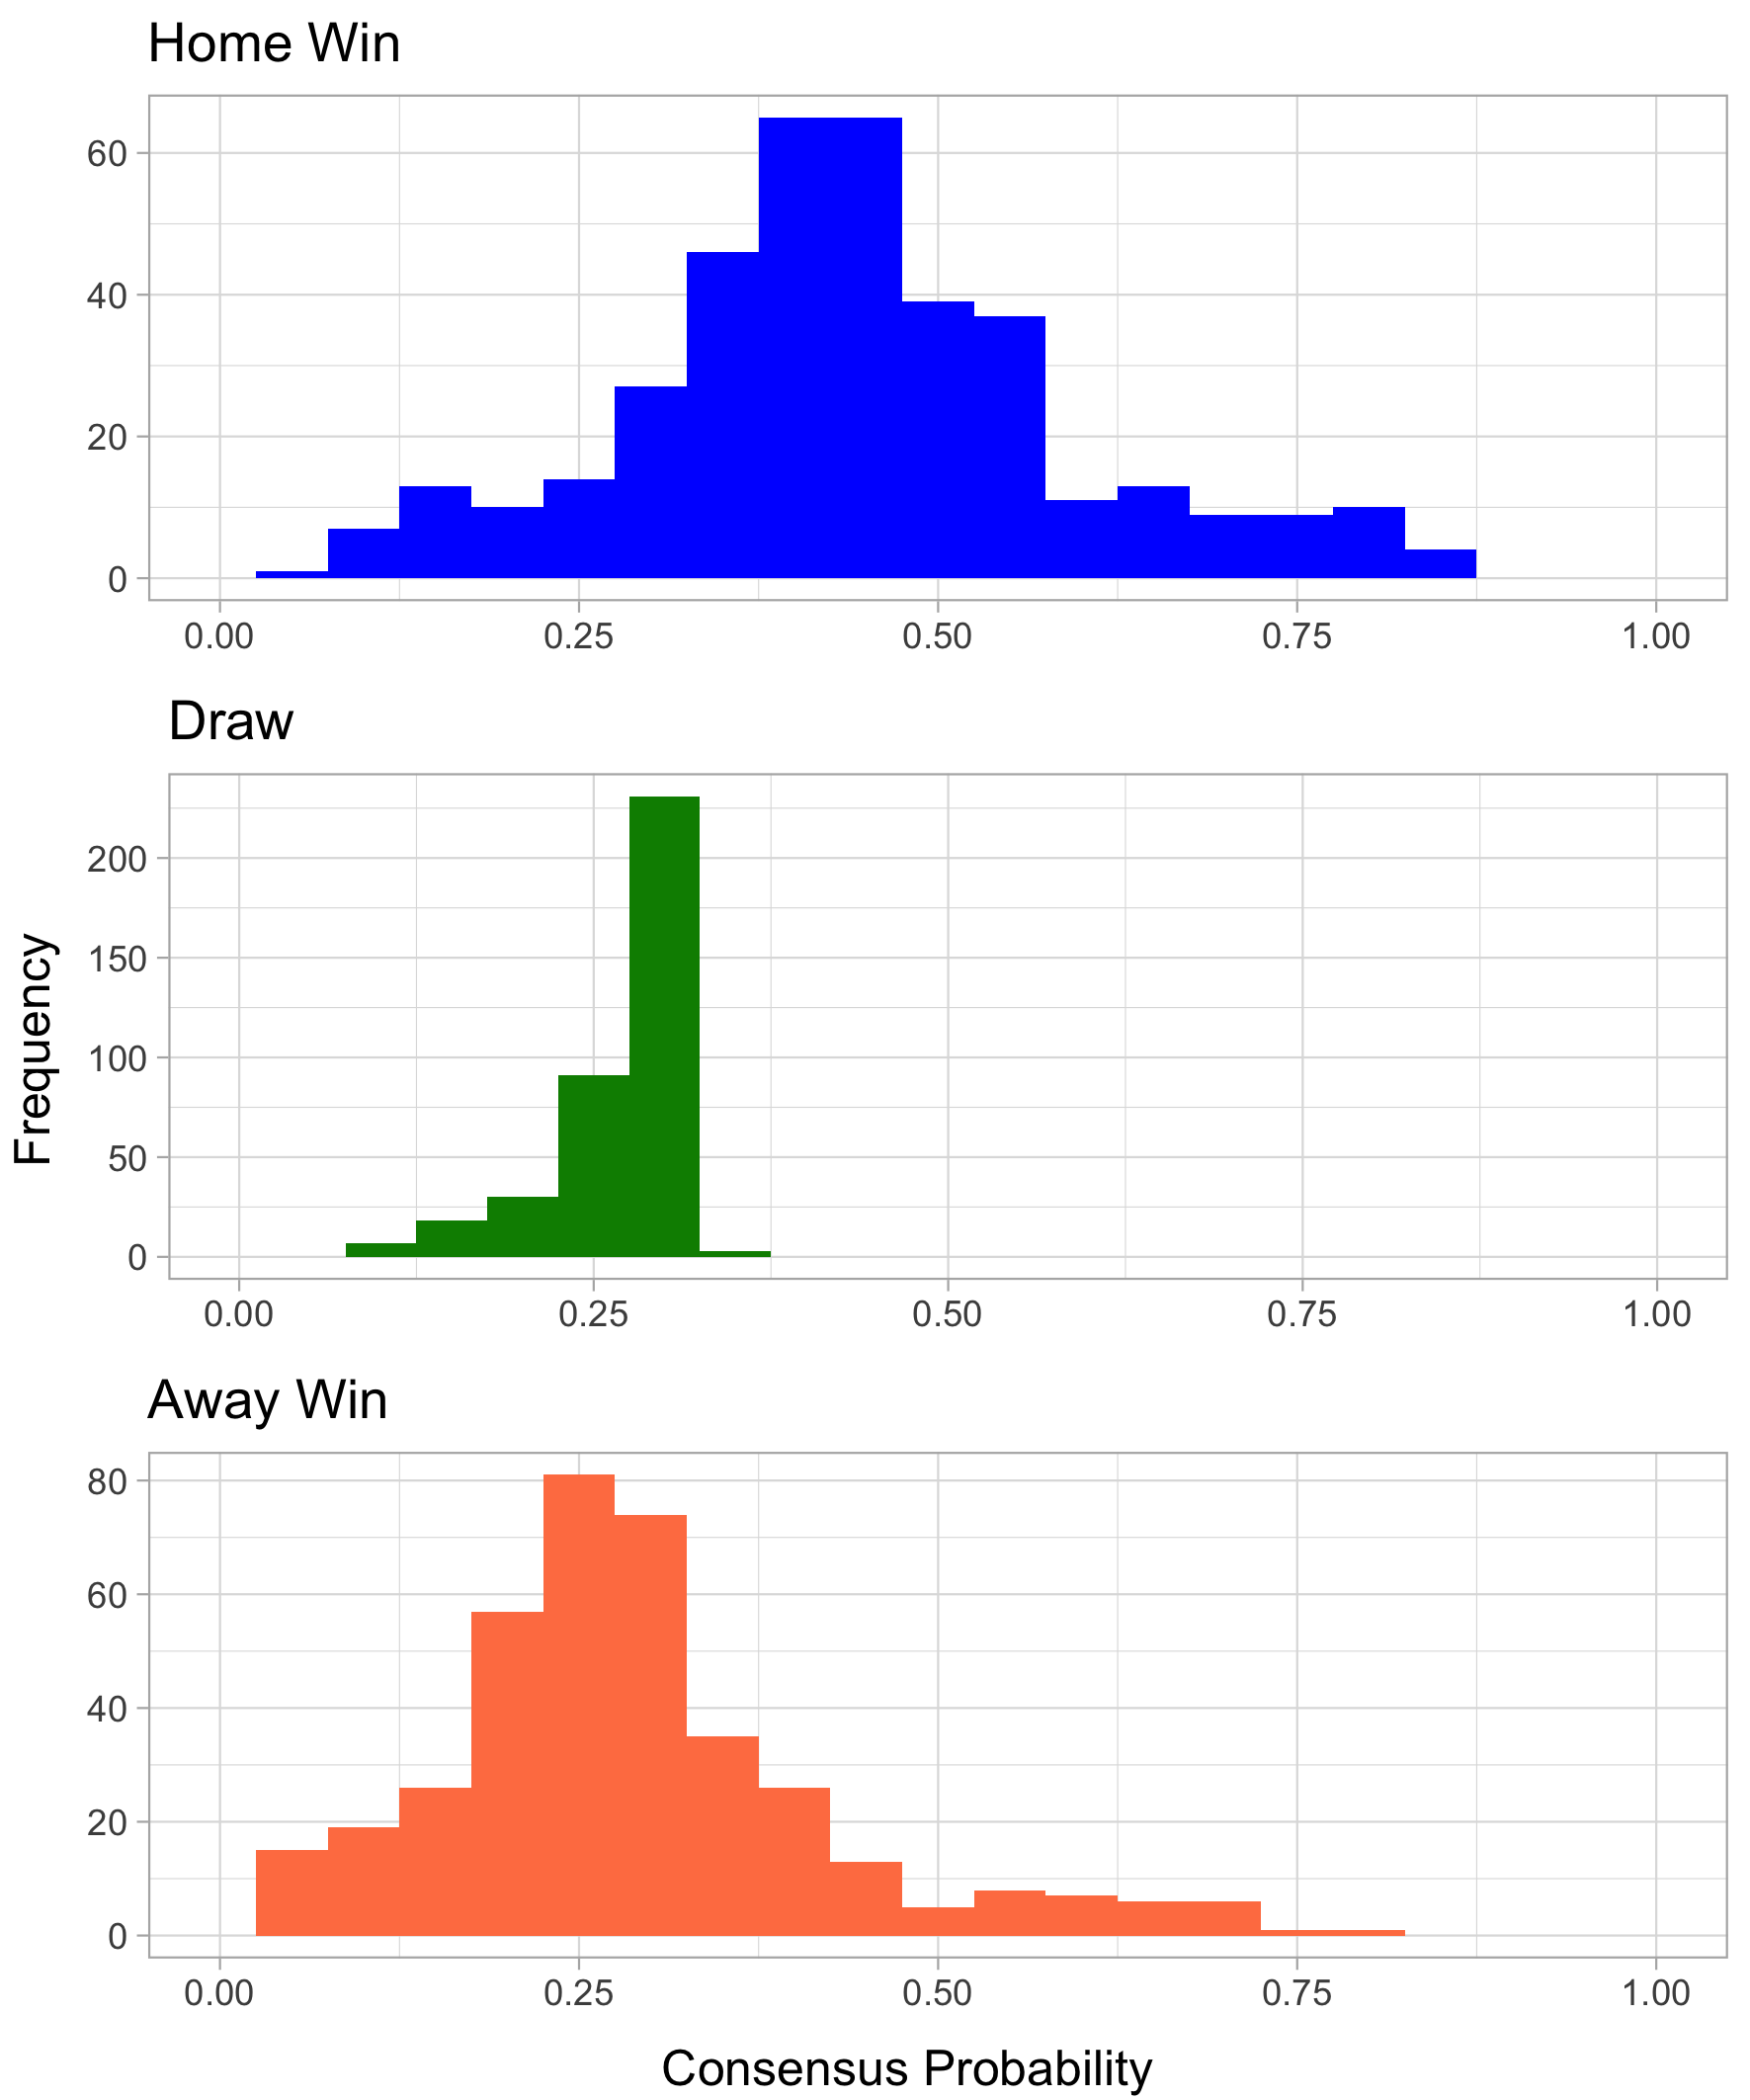
\includegraphics[width=0.7\textwidth]{elite_01_idahist.png}
	\caption{Histograms of the consensus probabilities for each outcome, in the French Ligue Une, 2016/17 season.}\label{FIG:01_01_idahist}
\end{center}\end{figure}

The figure shows that the consensus probabilities of a Home Win are symmetrically distributed around the mean $\mu_{\textrm{H}}=0.44$, with a distribution similar to the \textsc{Normal distribution} bell curve. The consensus probabilities of an Away Win are positively- (or right-) \textsc{skewed} suggesting a greater proportion of measurements are greater than/lie to the right of the peak value \autocite{Mendenhall13}. The data will, therefore, include a few  unusually large measurements. Contextually, these could be the league leaders playing away against a poor performing side.

The graph of the consensus probabilities of a Draw assists the finding (based on $\sigma_{\textrm{D}}$) that the variation of consensus probabilities of a Draw is very low: Over 225 (of a total of $n=380$ matches) of the games lie in the same bin\footnote{The width of all bins, or groups of data points, across all three histograms is 0.05.} with no values at all recorded above 0.4.\vspace{3mm}

The rationale behind conducting IDA was to answer the four questions set out previously about the quality of the data and measurements; whether the implementation of the study fulfilled the intention of the research design; and the characteristics of the sample \autocite{Ader08}. The quality of the data and measurements are both acceptable for this project: no measurements are missing, computations were completed, and plots produced without any issues. The question of the study will be able to be answered: access to the information required is available (consensus odds and actual results). The final question, about the characteristics of the sample, can be answered by saying that the data suggests the mean consensus probabilities are roughly equal to the observed probability for each outcome ($\mathbb{P}_{\textrm{cons}} \approx \mathbb{P}_{\textrm{obs}}$); bookmakers offer less variation on their odds for a Draw than for a clear winner; and the consensus probability of a Home Win is symmetric, whereas the consensus probability of an Away Win is positively-skewed.

\section{Exploratory Data Analysis}\label{sec:eliteeda}
In this section, the data is explored using various techniques motivated by four `major themes'.
\begin{itemize}
	\item \textbf{Displays}: reveal major features, outliers, non-linearities, discontinuities, skewness, \textsc{etc.} that calculations such as means, standard deviations and least square regressions cannot show.
	\item \textbf{Residuals}: defined as the observed data minus the fitted data, a clear pattern in the plot of the residuals vs. fitted values indicates improvement is possible.
	\item \textbf{Resistance}: dealing with outliers. If they are found, parallel tests (one with outliers; one without) can be ran and compared, testing the resistance of the data to the outliers (not dissimilar to the idea of statistical \textsc{leverage}).
	\item \textbf{Transformations}: does adding a transformation, such as taking the $n$-th root, logarithms, logits/probits, \textsc{etc.} allow sense to be made of the data? \autocite{Hoaglin77}
\end{itemize}

The data must first be read in and cleaned (as six leagues and 15 seasons---90 datasets---are being considered, it is efficient to use a \lstinline|for| loop to do this). The reasons for choosing these seasons are explained in Section~\ref{sec:aimsobjectives}. The code to do so---including finding the underlying probabilities, and to normalising to find consensus probabilities---is below.

\begin{lstlisting}
countries <- c("de", "en", "es", "fr", "it", "po")
co.we <- c("D1", "E0", "SP1", "F1", "I1", "P1") 
#n.b. The Premier League's code is 0; other countries are 1.
seasons <- c("0506", "0607", "0708", "0809", "0910", "1011", "1112", "1213", "1314", "1415", "1516", "1617", "1718", "1819", "1920")
eliteTemp <- NULL; elite <- NULL
for (i in seasons){
	for (j in 1:6){
		eliteTemp <- read.csv(paste0('https://www.football-data.co.uk/mmz4281/', i, '/', co.we[j],'.csv'), fileEncoding = 'latin1')
		eliteTemp$Country <- with(eliteTemp, countries[j])
		eliteTemp$Season <- with(eliteTemp, i)
		if (i=="1920"){
			eliteTemp$BbAvH<-eliteTemp$AvgH; eliteTemp$BbAvA<-eliteTemp$AvgA
			eliteTemp$BbAvD<-eliteTemp$AvgD
		}
		else{}
		eliteTemp <- eliteTemp[ ,c("Div", "Date", "HomeTeam", "AwayTeam", "FTHG", "FTAG", "FTR", "BbAvH", "BbAvD", "BbAvA", "Country", "Season")]
		elite <- rbind(elite, eliteTemp)
	}
}
elite <- na.omit(elite)

#Finding underlying probabilities: 
#Pre-Normalised Probabilities
elite$AvgHProbPN <- with(elite, round(1/BbAvH, 4)) 
elite$AvgDProbPN <- with(elite, round(1/BbAvD, 4))
elite$AvgAProbPN <- with(elite, round(1/BbAvA, 4))
#To normalise them:
elite$overround<-with(elite, (AvgHProbPN + AvgDProbPN + AvgAProbPN))
elite$AvgHProb <-with(elite, round(AvgHProbPN/overround, 4))
elite$AvgDProb <-with(elite, round(AvgDProbPN/overround, 4))
elite$AvgAProb <-with(elite, round(AvgAProbPN/overround, 4))
\end{lstlisting}

The number of matches in the dataset $N = 31,346$; as this is large, the \textsc{central limit theorem} (CLT) can be applied, allowing the assumption that the mean of the random variables (contextually, matches) follows the Normal distribution. For later analysis, the \textit{correct} probability (and the natural logarithm of it) (the bookmaker consensus probability of the event that was observed) and the two \textit{incorrect} probabilities need to be found also.

The first step after cleaning the data is to compute the consensus mean probabilities and compare them to the observed probabilities for each market $m$. These are shown in Table~\ref{tab:edaelitecalcs}.\vspace{3mm}

\begin{table}[h!]\begin{center}\begin{tabular}[h!]{c||c|c|c}
	& \textit{Home Win} & \textit{Draw} & \textit{Away Win} \\\hline\hline
	Mean Consensus Probability $\mu_m$ & 0.4472 & 0.2620 & 0.2908 \\
	Observed Probability& 0.4589&0.2566 & 0.2845\\\hline
	Consensus Standard Deviation $\sigma_m$&0.1714&0.0478&0.1536
\end{tabular}\end{center} \caption{Basic calculations for the entire \textit{elite} dataset, forming part of the exploratory data analysis.} \label{tab:edaelitecalcs}\end{table}

As seen in Table~\ref{tab:idacalcs}, the mean consensus probabilities are extremely close to the observed probabilities: the magnitude difference is than 0.02 for all three outcomes. Similarly, the standard deviations indicate that the consensus probabilities offered for a Draw vary significantly less than for those with a clear winner. \vspace{3mm}

Visual analyses are used; namely, box, density, and tile plots. First, a boxplot for each outcome is created, to assess whether there is a significant difference, or there exists a trend, in the observed outcome for the bookmaker probabilities of each event. These are shown in Figure~\ref{FIG:01_02_bp}.

\begin{figure}[h!]\begin{center}
	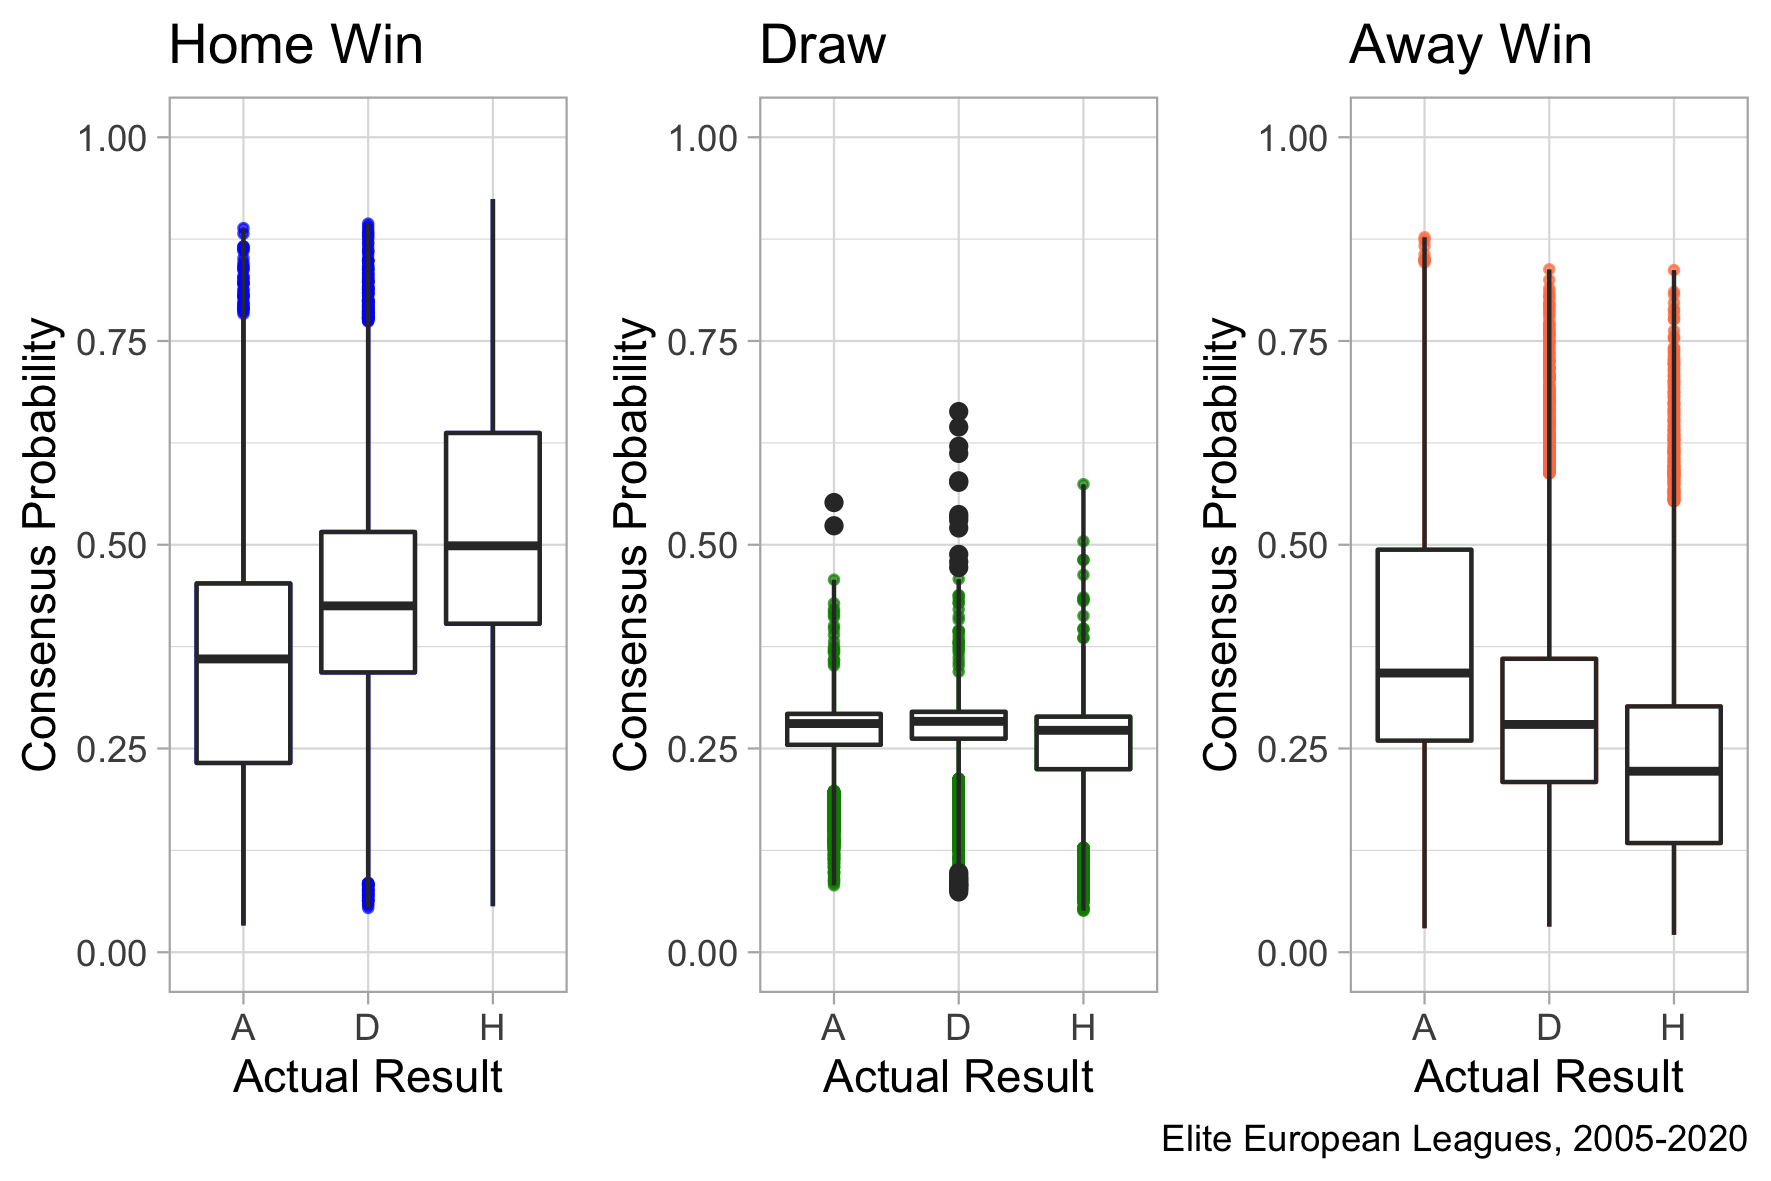
\includegraphics[width=0.8\textwidth]{elite_02_boxplot.png}
	\caption{Boxplots of the consensus probabilities offered for each outcome.}\label{FIG:01_02_bp}
\end{center}\end{figure}

The figure implies there is no significant difference: whilst it appears there is a correlation---for games that end in Home Wins, the consensus probability of a Home Win is higher, and vice versa for Away Wins---this plot shows no strong significance; however, it does strongly reiterate the aforementioned point about variation (or lack thereof) of the consensus probabilities of a Draw. The Draw plot has a large number of outliers; these are considered later.\vspace{3mm}

Instead of creating a binned histogram, as in Figure~\ref{FIG:01_01_idahist}, a density plot is used, allowing for an easier visualisation of the data, and easier comparisons between leagues. Using \textsc{kernel density estimation}, the data that would be used to create a histogram is `smoothed out' using a number of equally spaced points at which the density (rather than the frequency, as in a histogram) is estimated. The plot for Home and Away Wins together is achieved using the code below; Draws are plotted separately due to a different $y$ axis scale being used. This results in Figure~\ref{FIG:01_02_edadensall}.

\begin{lstlisting}
ggplot(elite, aes(x=AvgHProb, color="Home Win")) + geom_density() + geom_density(data=elite, mapping=aes(x=AvgAProb, color="Away Win"), show.legend=T) + coord_cartesian(xlim=c(0,1)) + labs(title="Home and Away Wins", caption="Elite Leagues, 2005-2020", x="Consensus Probability", y="Density") + theme_light() + scale_color_manual(name="Market", values=c("Home Win" = "blue", "Away Win" = "coral"))
\end{lstlisting}
\vspace{3mm}
\begin{figure}[h!]\begin{center}
	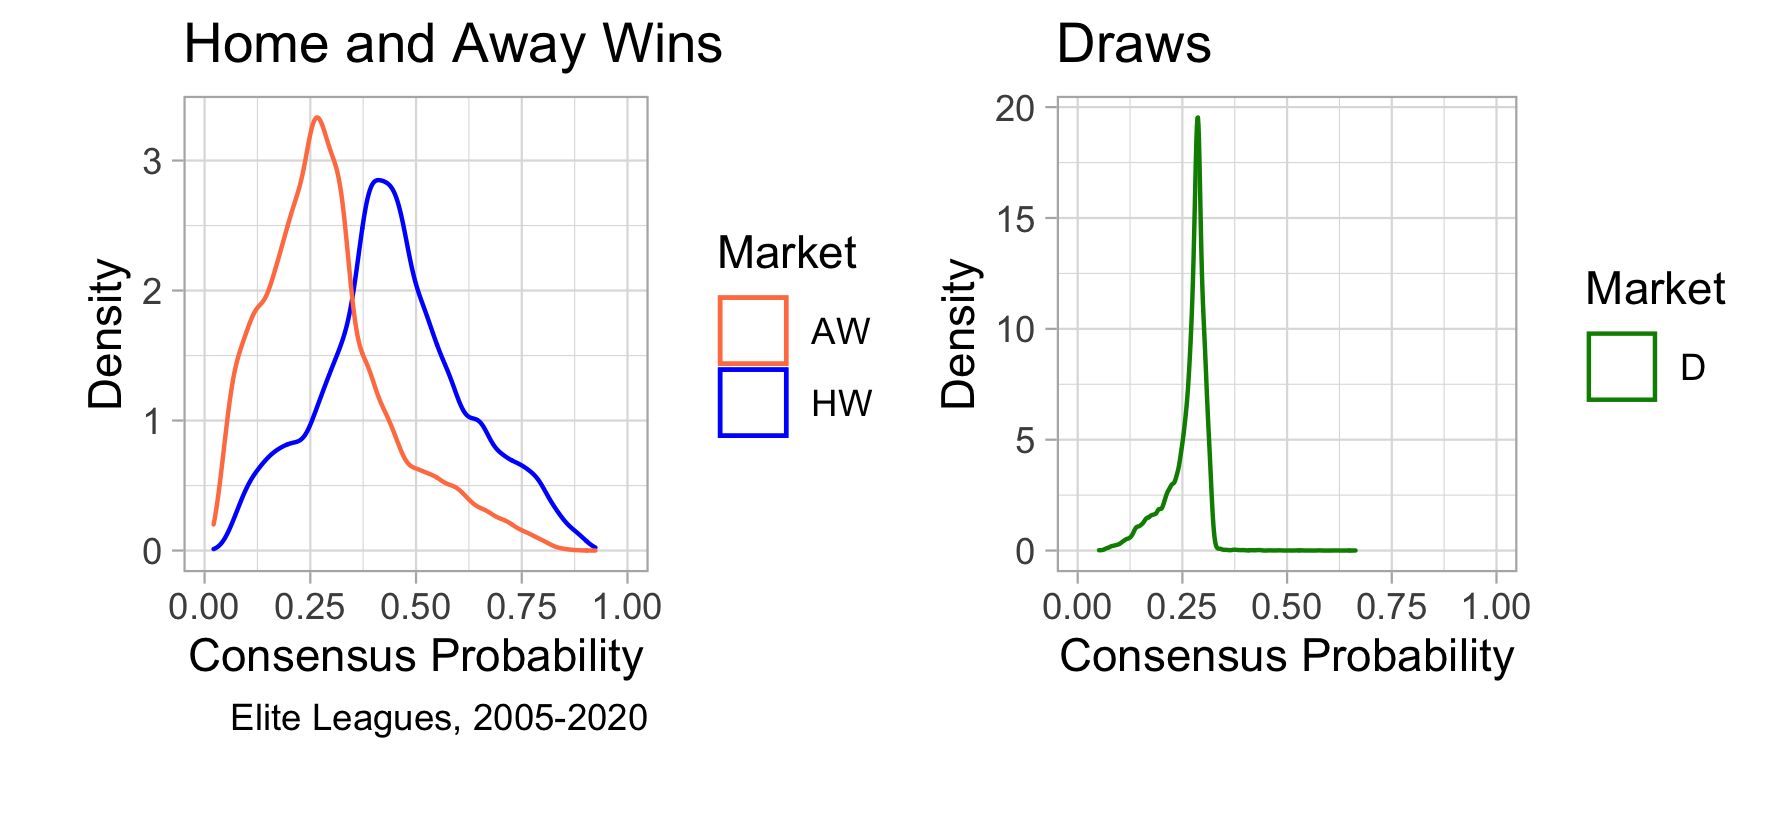
\includegraphics[width=\textwidth]{elite_02_edadensall.png}
	\caption{Density plots of the consensus probabilities offered for each outcome in the 1X2 market.}\label{FIG:01_02_edadensall} 	
\end{center}\end{figure}

Interpreting this figure shows the trend shown from still holds: $\mathbb{P}_{\textrm{cons}}$(Home Win) is symmetrically distributed around the peak ($\mu_{H}=0.45$); $\mathbb{P}_{\textrm{cons}}$(Away Win) has a positive skew; and $\mathbb{P}_{\textrm{cons}}$(Draw) has much less variation, with few matches above the peak. 

An interpretation of this figure shows the trend from Figure~\ref{FIG:01_01_idahist} remains. The consensus probabilities of a Home Win are symmetrically distributed around the mean ($\mu_{H}=0.45$); the consensus probabilities of an Away Win have a positive skew; and the consensus probabilities of a Draw have much less variation, with few matches above the mean. Reviewing the latter, Table~\ref{tab:highprobdraws} shows matches with a consensus probability of a Draw greater than 0.6, where 0.6 is seven standard deviations away from the mean consensus probability of a Draw. 

\begin{table}[h!]\begin{center}\begin{tabular}[h!]{c|c||c|c|c||c}
	\textit{League} & \textit{Date} & \textit{Home Team} & \textit{Away Team} & \textit{Final Score} & $\mathbb{P}_{\textrm{cons}}(\textrm{Draw})$ \\ \hline \hline
	Serie A & 09/05/10 & Bologna	& Catania 	& 1-1 & 0.6634 \\
	Serie A & 08/05/11 & Bologna 	& Parma 	& 0-0 & 0.6445 \\
	Serie A & 20/05/07 & Torino	 	& Livorno 	& 0-0 & 0.6208 \\ 
	Serie A & 03/04/11 & Chievo 	& Sampdoria & 0-0 & 0.6121
\end{tabular}\end{center}\caption{Matches with consensus probability of a Draw,  $\mathbb{P}_{\textrm{cons}}(\textrm{Draw})>0.6$}\label{tab:highprobdraws}\end{table}

All these matches are both a) in the Italian Serie A; and b) in the late stages of the football season.\footnote{The season normally starts in August and ends in May \autocite{PremierLeagueHandbook}.} There are two possible reasons for this.
\begin{itemize}
	\item The Italian Serie A has a history of match fixing in recent times: the \textsc{Calciopoli}, which occurred during the 2004/05 and 2005/06 season involved Juventus, AC Milan, and Lazio, among others---three of Italy's largest clubs \autocite{Calciopoli}; and in 2015, Catania's president was one of several arrested for match-fixing in Serie B matches \autocite{catania}.
	\item Due to these games occurring in the late stages, it is possible for a scenario to arise where both teams would benefit from a certain result.\footnote{The \textsc{Disgrace of Gijón} in the 1982 World Cup is a particularly famous example of this (See Appendix~\ref{app:definitionsgambling}, Definition~\ref{def:disgraceofgijon}).}
\end{itemize}

Whilst fixed matches would naturally impact the results, due to the small number of games impacted, it is unnecessary to exclude them from future analysis. As these games are all in the Serie A (a further investigation reveals, of the 81 matches in the dataset with a consensus probability of a Draw greater than 0.35, 75 (93\%) were Italian matches), it makes sense to split this density plot into the different leagues, shown in Figure~\ref{FIG:01_02_edadensleagues}.

The Home Win (and to a lesser extent Away Win) plots imply leagues can be split into two categories: those with a \textit{unimodal} distribution (one local \textsc{mode}/peak), and those with a \textit{trimodal} distribution (three local modes/peaks). The latter group (England, Portugal, Spain) have a peak between 0 and 0.25 (very low probability of a Home/Away win, depending on the plot) and a peak between 0.75 and 1 (very high probability of a Home/Away win), whereas the former (Germany, France, Italy) only has the central peak. One reason could be competitive balance, investigated further in Section~\ref{sec:elitecompbal}.

\begin{figure}[h!]\begin{center}
	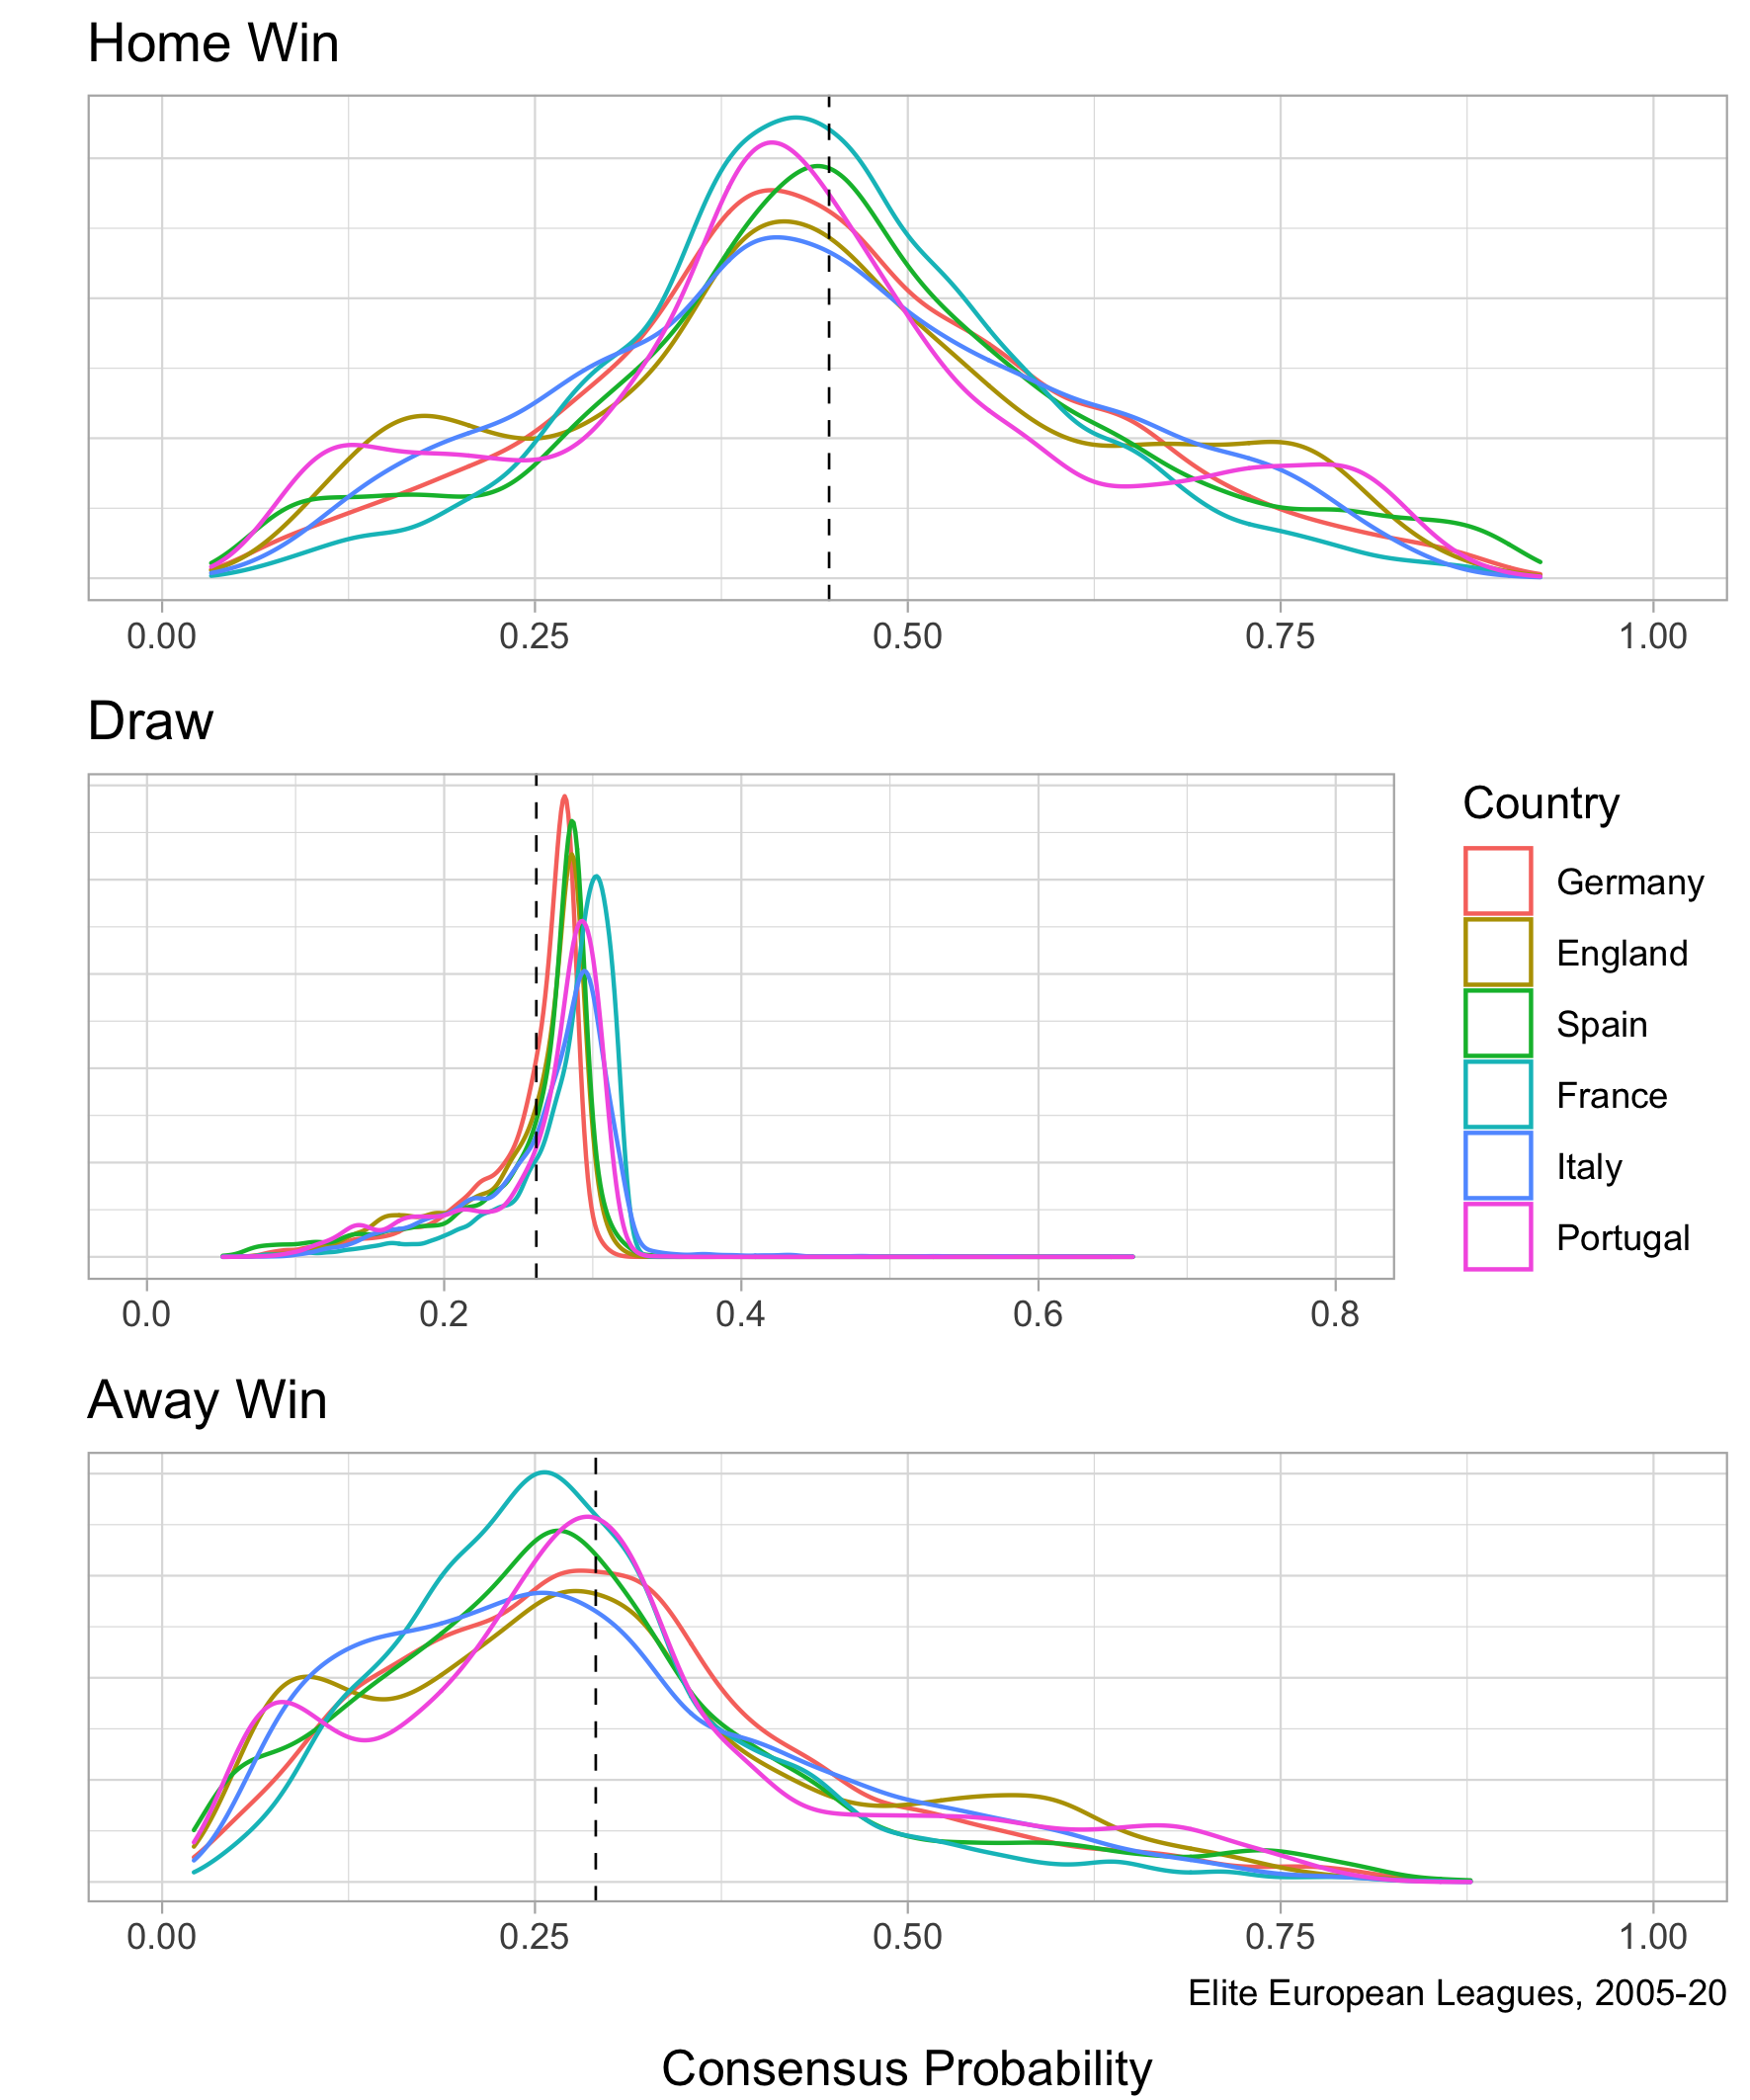
\includegraphics[width=0.7\textwidth]{elite_02_edadens.png}
	\caption{Density plots of the consensus probabilities offered for each outcome of the 1X2 market, split by league.}\label{FIG:01_02_edadensleagues}
\end{center}\end{figure}\vspace{3mm}

The final visual aid used in this section is a tile plot. Similar to a heat map, this will allow for a three-dimensional representation of data in the two-dimensional plane. The match goals will be plotted on the $x$ (Home goals) and $y$ (Away goals) axes, which allows for the full-time result to be shown, (tiles on the diagonal $x=y$, are Draws; upper triangle are Away Wins $y>x$; lower triangle are Home Wins $x>y$) and the \textit{magnitude} of the result, or how \textit{convincing} the result is: a match further from the diagonal has a greater disparity in goals, and so can be considered a more convincing win. Representing the $z$ axis, each square will be shaded in with the mean \textit{correct} consensus probability for that result: with a low consensus probability, the square will be lighter. 

It is expected these to be closer to the diagonal. Due to a low number of extreme results where more than 5 goals are scored by a team, these are grouped these into a 5+ tile.\footnote{The highest scoring draws were 5--5, occurring twice: Lyon vs. Marseille (2009) and West Bromich Albion vs. Manchester United (2013).} The bin sizes (number of matches with a given result) are given in Table~\ref{tab:tilebinsizes}.

\begin{table}[h!]\begin{center}\begin{tabular}[h!]{cc|cccccc}
\parbox[t]{2mm}{\multirow{6}{*}{\rotatebox[origin=c]{90}{Away Goals}}}
&	5+ 	& 119 	& 105	& 67	& 26 	& 7 	& 2 \\
&	4 	& 257  	&294  	&174 	&  63 	&  36 	& 12 \\
&	3	& 636 	& 869 	& 547  	& 299  	&109	& 45 \\
&	2	&1451 	&2003 	&1508 	& 712 	& 265 	& 106 \\
&	1	&2299 	&3688 	&2756 	&1375  	&528 	& 281 \\
&	0	& 2510 	&3342 	&2575 	&1371 	& 594 	& 315 \\ \hline
&& 0 	& 1 	& 2 	& 3 	& 4 	& 5+\\
&&\multicolumn{6}{c}{Home Goals}
\end{tabular}\end{center}\caption{The bin size for each tile in Figure~\ref{FIG:01_05_tile}.}\label{tab:tilebinsizes}
\end{table}

\begin{figure}[h!]\begin{center}
		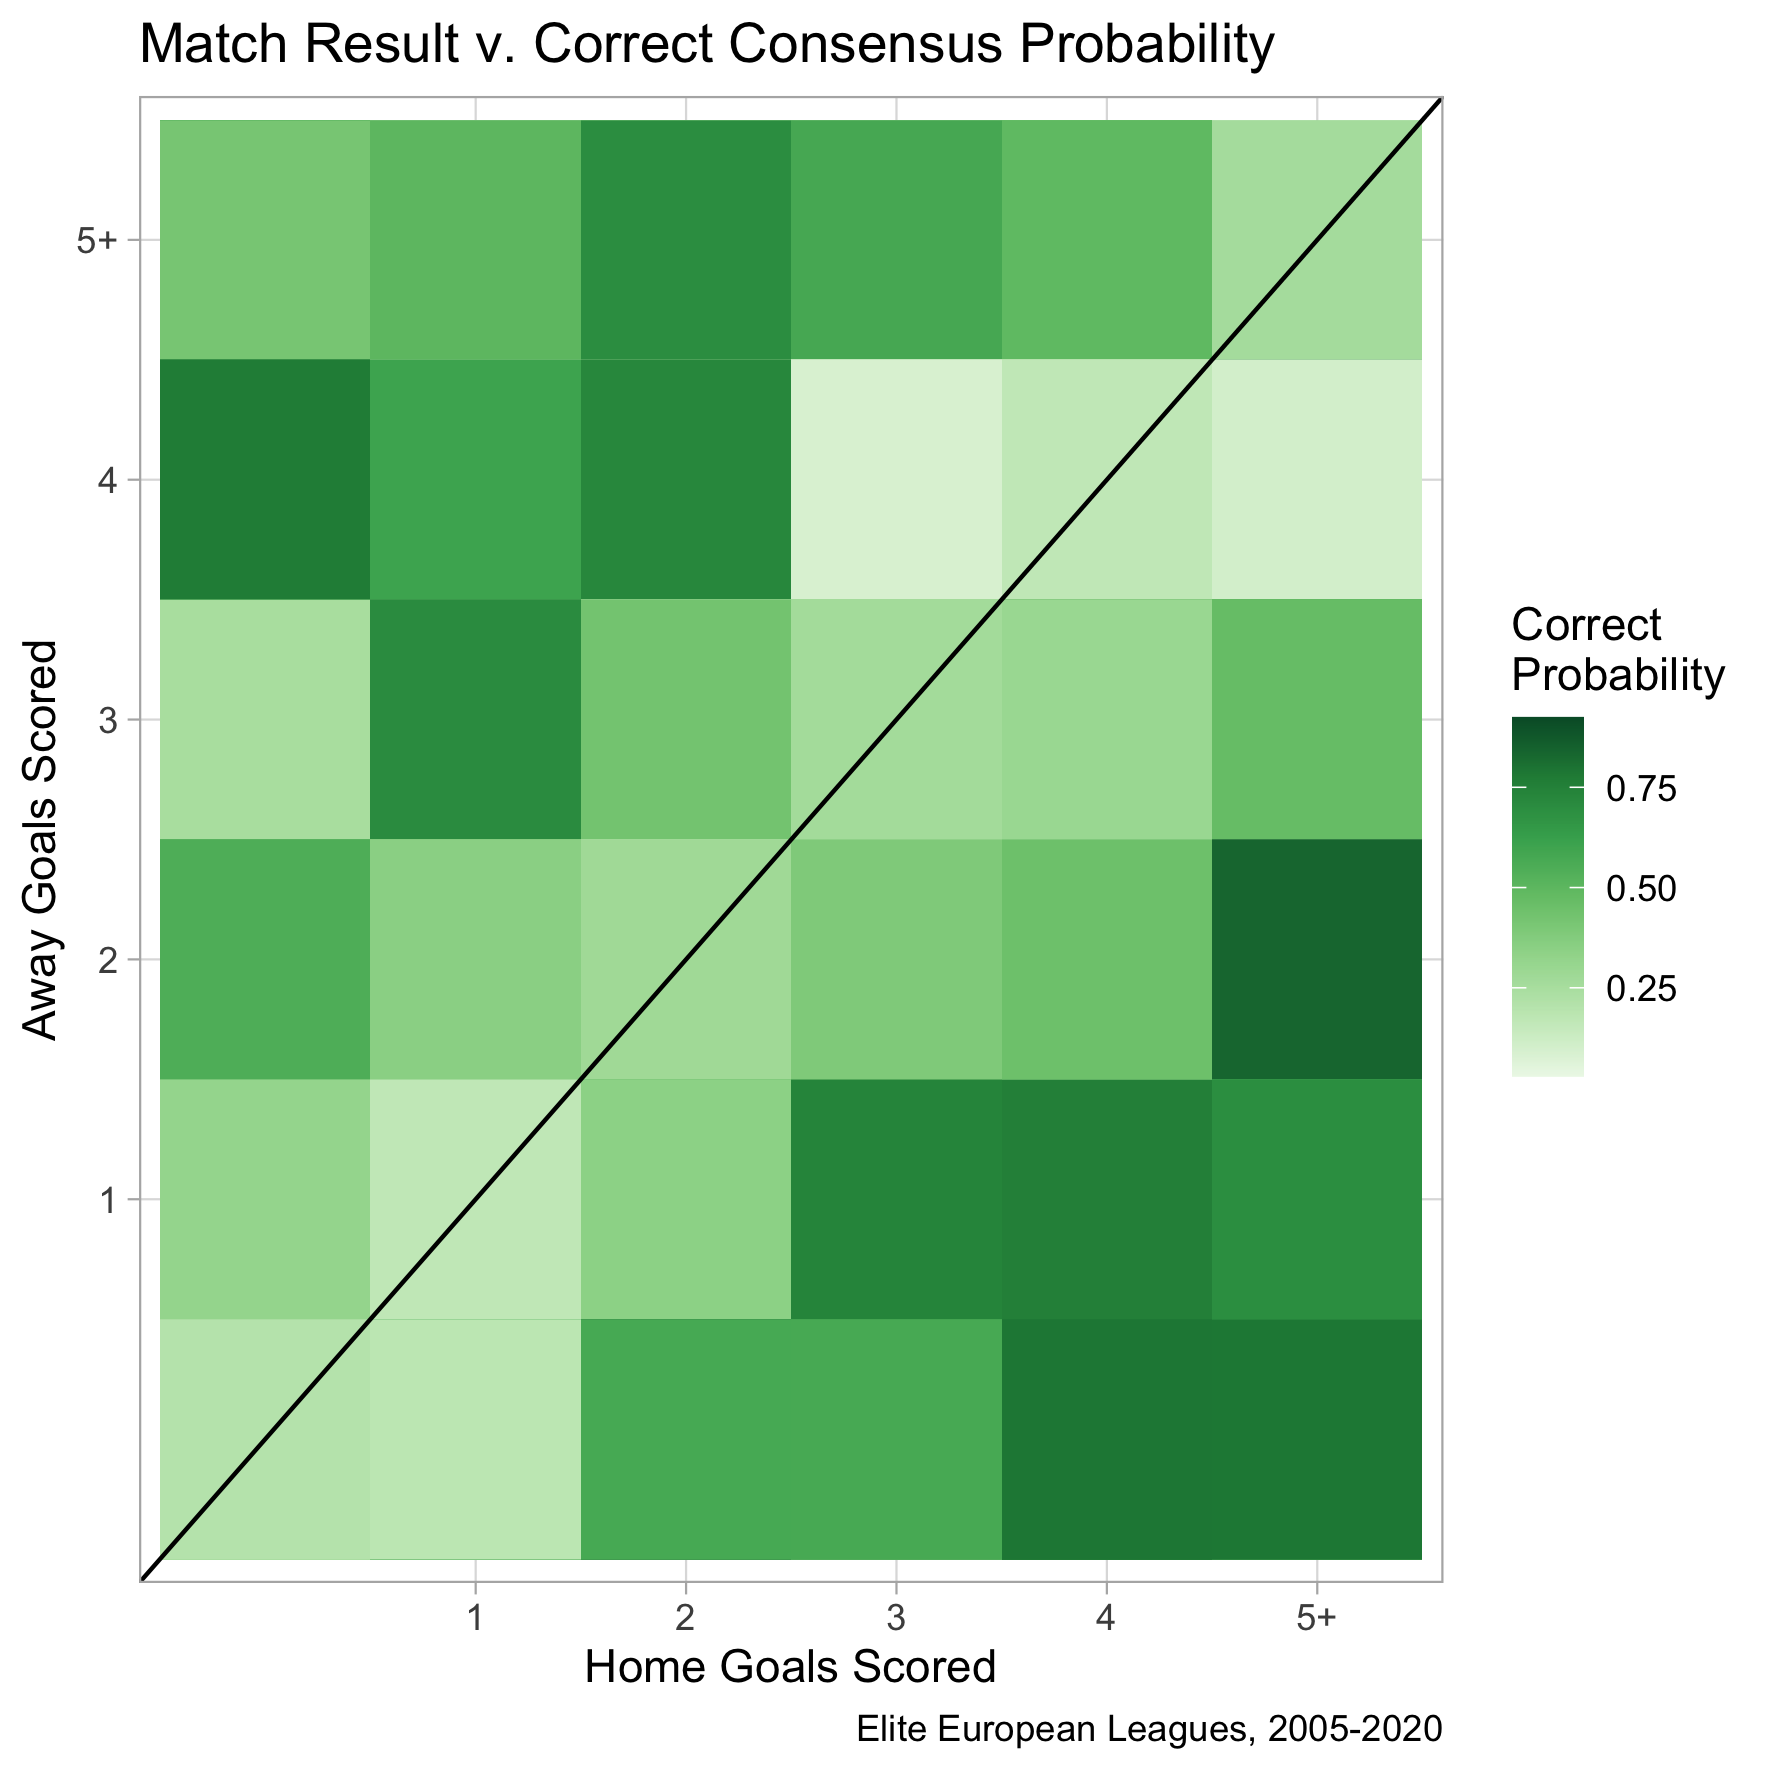
\includegraphics[width=0.7\textwidth]{elite_05_tile.png}
		\caption{Tile plot of the correct consensus probability for each possible result.}\label{FIG:01_05_tile}
\end{center}\end{figure}

The results on the diagonal all have a similar consensus probability, around 0.3. This is unsurprising, given the low variation in the consensus probabilities of Draws. Considering the lower triangle (Home Wins) first, the pattern expected holds: that is, tiles furthest from the diagonal are darker. Interestingly, the darkest tile is for a 5+ -- 2 Home Win; the bin size for this is low, however, with $n=106$ matches.\footnote{0.0034\% of the total dataset.} Whilst there are only 12 games in the 5+ -- 4 tile, it is striking that it has one of the lowest correct consensus probabilities of all the tiles. Considering the upper triangle (Away Wins), the pattern is not as consistent as with Home Wins, but there is still evidence of it, with the highest probabilities being further from the diagonal. As a whole, the figure is implying games with greater disparity in full-time goals (\textsc{i.e.}, more convincing wins) have a higher bookmaker consensus probability of the correct result.

It is worth noting that more ideal measures of how convincing a match is exist, such as `Expected Goals' (xG), a metric commonly used to evaluate the offensive-effectiveness of players, which can be used to create an `Expected Results' and `Expected League Tables', by giving each shot a theoretical goal value based on historical shots from the same location, angle, position of defenders, goalkeeper positioning, \textsc{etc}. \autocite{xgoals, xgoals2}.\vspace{3mm}

EDA was conducted to check four themes: displays, residuals, resistance, and transformations.
\begin{itemize}
	\item Displays: Whilst there was no discontinuity--as in the IDA in Section~\ref{sec:eliteida}---the consensus probabilities of Away Wins are positively/right-skewed, and of Draws have a very low \textsc{variance}. The outlying matches with a large $\mathbb{P}_{\textrm{cons}}$(Draw) were assessed.
	\item Residuals \& Resistance: Models have not been created (this is done in Section~\ref{sec:elitecorr}), so the residuals cannot be plotted. 
	\item Transformations: The data makes sense, and is as expected. There is nothing in the plots to suggest the need of, or to justify the use of, any transformations.
\end{itemize}


\section{Correlation Analysis and Linear Model Creation}\label{sec:elitecorr}
In this section, the coefficient of determination $R^2$ and the root-mean-square-error RMSE are found. This is done by creating a linear model to predict the observed probability (denoted $\mathfrak{O}$) from a given consensus probability ($\mathfrak{C}$). Linear models are chosen as the `ideal' relationship between the observed and consensus probabilities is a $y=x$ line, where a bookmaker prediction of 0.25, for example, would correlate with an observed probability of 0.25. For the $i^{\textrm{th}}$ match (observation), the model created, in a set market, is of the form given in Equation~\ref{eq:linearmodel}, where $x_0$ is the intercept, $x_1$ is the \textit{slope}, or gradient, of the line, $\mathfrak{C}_i$ is the consensus probability of the $i^{\textrm{th}}$ match, and $\epsilon_i$ is the error (residual) for that match.

\begin{equation}\label{eq:linearmodel}
\mathfrak{O}_i = x_0 + x_1\cdot\mathfrak{C}_i + \epsilon_i
\end{equation}

The RMSE for each game is defined as the square root of the mean residual point (the distance from each data point to the linear model created) squared. $R^2$ lies between 0 and 1, and is defined in Appendix~\ref{app:definitions}, Definition~\ref{def:coeffofdet}. High levels of correlation will result in a high $R^2$ and accurate models result in low RMSE values \autocite{Mendenhall13}. There are alternatives to RMSE, such as mean square error, mean absolute error, median absolute error, and computing the distance from a point to the `ideal' line: RMSE is more sensitive to outliers than mean and median absolute error; RMSE is chosen due to a relatively low amount of variation in values,\footnote{A caveat of RMSE is that it gives more weight to large errors, as the errors are squared. RMSE therefore is more useful when large errors are `undesireable' \autocite{maevrmse}.} and its greater theoretical relevance \autocite{Hyndman06}. $R^2$ describes the percentage of the variation in a dependant variable---in this case, the observed probability---due to a predictor---the bookmaker consensus probability \autocite{Draper98}.

The slope of the line can be used as an indicator of fit, too. As the `ideal' model is known, a comparison between the fitted model $x_1$ and the ideal slope (1) can be made. The magnitude or percentage deviation could be used to check for discrepancy, regardless of whether the fitted model is steeper or shallower, which counters problems that may occur due to a pattern that oscillated above and below the ideal, however, the strict slope will be considered in this project, as such a trend would be of interest. \vspace{3mm}

In addition to an overall $R^2$, RMSE, and slope, the three values for each \textit{elite} league will be found, and used in Section~\ref{sec:elitecomparingleagues}. 

This is conducted by \textit{binning} matches, where the data is partitioned into groups (bins), with a sufficient amount to `capture the major features in the data while ignoring fine details' \autocite{knuth06}. Games with similar consensus probabilities for a given outcome will be binned together, before the observed proportion of games in the bin with that outcome is found, which is referred to as the observed probability $\mathbb{P}_{\textrm{obs}}$(Outcome). This is used to find the consensus vs. observed probabilities in future analysis (plots and model creations). In R, bins are created using the \lstinline|cut| function, and the \lstinline|tapply| function is used to find the mean value in each bin.\footnote{The default is the midpoint \autocite{cutdocumentation}.} The R code used for the Home Wins is below. 124 breaks (cut-points) are chosen, meaning that each bin has over 250 matches. Doing this for each outcome and overall results in the $R^2$, RMSE, and slope values presented in Table~\ref{tab:overallrsqrmse}.

\begin{lstlisting}
elite$AvgHProb.cut <- cut(elite$AvgHProb, 124, include.lowest=T)
#First, we cut the data into 'bins' choosing 124 breaks
levels(elite$AvgHProb.cut) <- tapply(elite$AvgHProb, elite$AvgHProb.cut, mean)
#Tapply finds the mean of the bin, rather than taking the midpoint
elite.observed.probabilites.TabH <- prop.table(table(elite$FTR, elite$AvgHProb.cut), 2)[c(1, 2, 3),]
#The c(1,2,3) will remove any extra (blank) rows
elite.observed.probabilites.H <- elite.observed.probabilites.TabH[3,] 
#[n,]; if n = : 1 Away; 2 Draw; 3 Home (alphabetic)
elite.bookmaker.probabilites.H <- as.numeric(names(elite.observed.probabilites.H))
\end{lstlisting}

\begin{table}[h!]\begin{center}\begin{tabular}[h!]{c||c|c|c||c}
		&\textit{Home Win}	& \textit{Draw}	&\textit{Away Win}	&\textit{Overall}\\\hline\hline 
$R^2$ 	& 0.98665 			& 0.52008 		& 0.96411 			& 0.83832 \\
RMSE 	& 0.03241 			& 0.20767 		& 0.05166 			& 0.11768 \\
Slope	& 1.08278			& 1.38142		& 1.09182			& 1.11148
\end{tabular}\end{center}\caption{$R^2$, RMSE, and Slope values for the \textit{elite} leagues, 2005--20.}\label{tab:overallrsqrmse}
\end{table}

These values show that, for the Home and Away Win models, a strong correlation ($>95\%$) exists between the consensus and observed probabilities.\footnote{For a perfect correlation, $R^2=1$, 100\% \autocite{Mendenhall13}.} In addition, the RMSE values for the two are very low: 0.03 for Home Wins and 0.05 for Away Wins, and the slopes are both less than 0.1 off the ideal. For Draws, $R^2 = 52\%$, RMSE $= 0.21$, and the slope is 1.38, indicating that the consensus probabilities, and thus the bookmaker's odds, are not as accurate than they are as for clear results; this explains why the overall values indicate worse performance than Home and Away Wins, with $R^2 = 83.8\%$, RMSE $= 0.12$, and the slope is 1.11.

A further demonstration of this point is given in Figure~\ref{FIG:01_03_scatter}: a scatter plot of the observed probability vs. bookmaker consensus probability using the bins created. This is presented along with the linear models (and their corresponding 95\% \textsc{confidence intervals} (CIs) in light grey). The `ideal' $x=y$ line is included for reference (dashed black).

\begin{figure}[h!]\begin{center}
	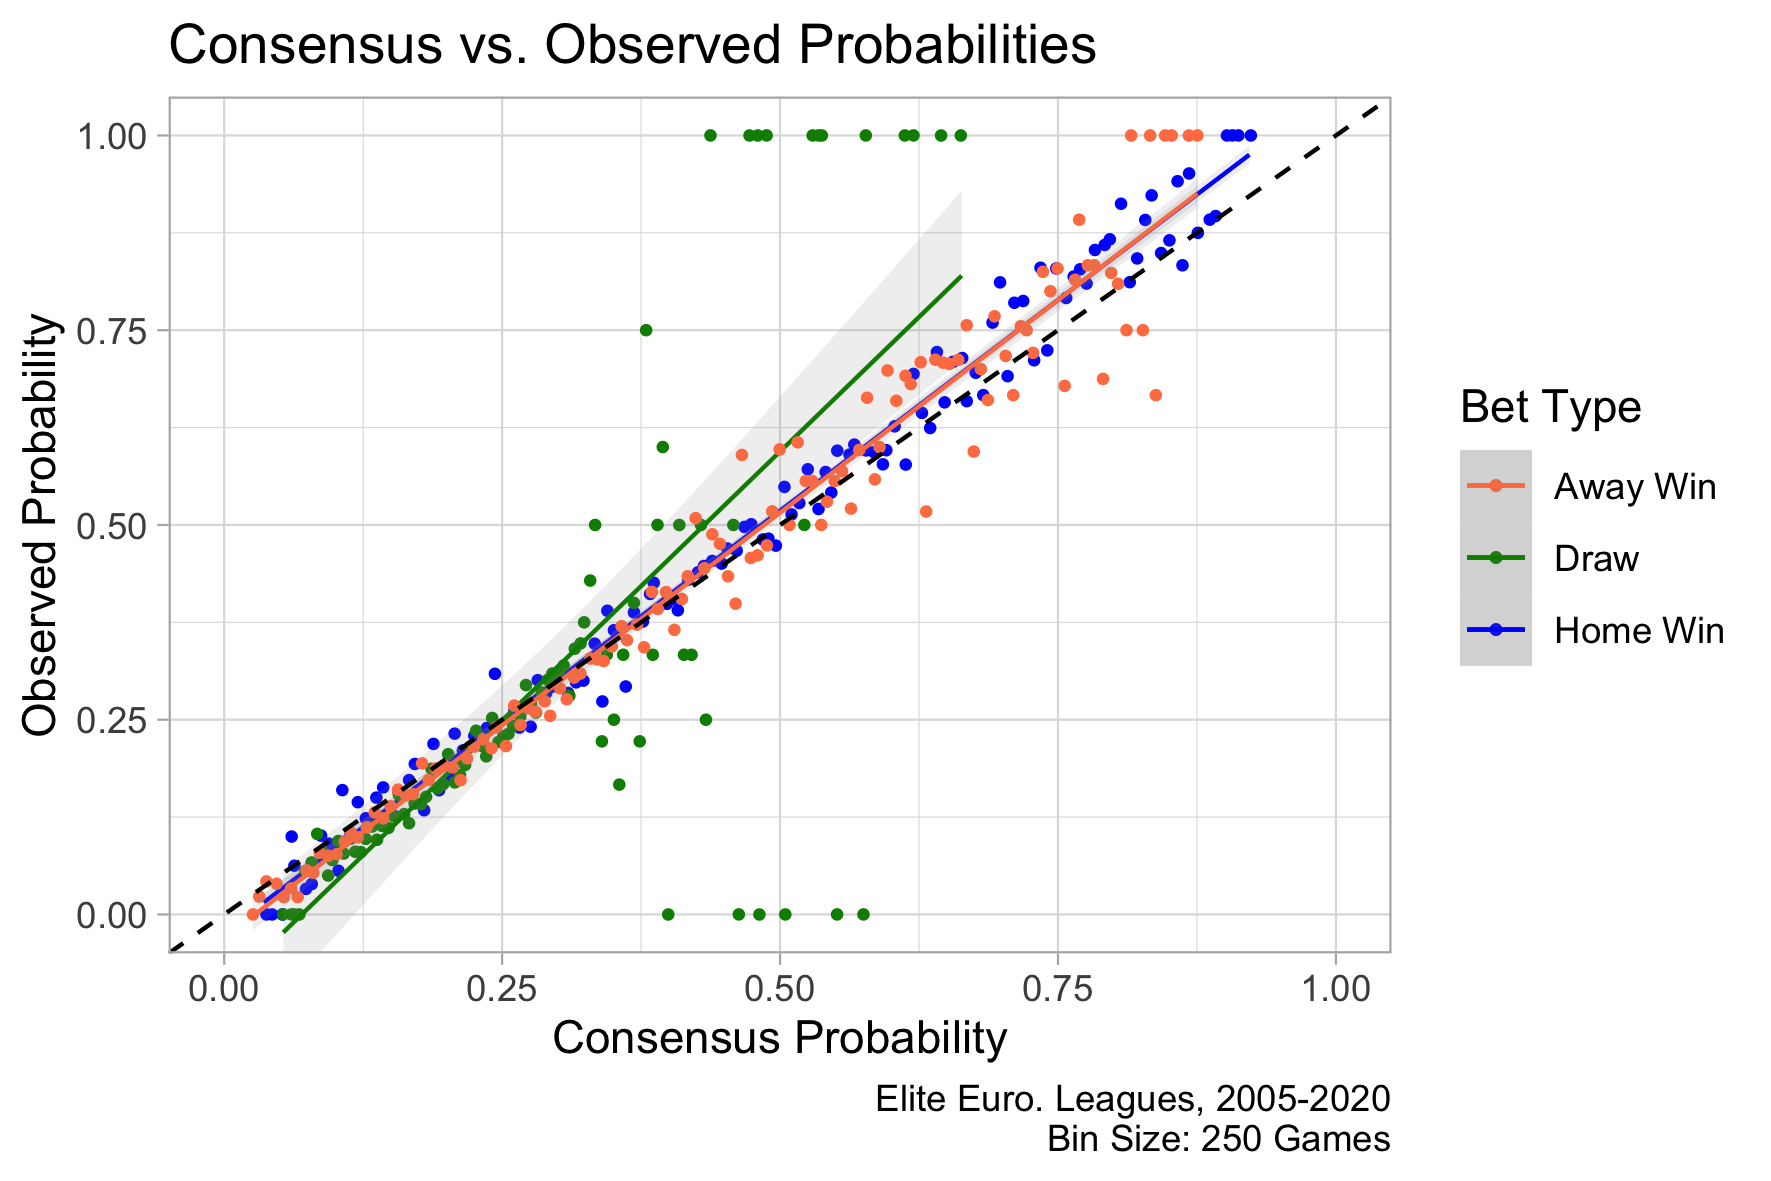
\includegraphics[width=0.8\textwidth]{elite_03_scatter.png}
	\caption{Scatter plot of the linear models created, showing the consensus probabilities vs. the observed probabilities.}\label{FIG:01_03_scatter}
\end{center}\end{figure}

The figure affirms the observations from the values in Table~\ref{tab:overallrsqrmse}, suggesting bookmaker accuracy for Home and Away Wins is extremely high. Both the 95\% CIs are extremely small, with no major outliers. The plot reiterated the poor bookmaker performance for Draws, with a large 95\% CI. It is also worth noting that the accuracy is higher for $\mathbb{P}_{\textrm{cons}}$(Draw) $\in(0,0.3)$ (within the range 0 to 0.3) and remarkably poor for consensus probabilities above this range: this coincides with the straight drop in density in consensus probabilities of a Draw in Figure~\ref{FIG:01_02_edadensall}. The values on the $y=1$ line---where all games in the bin were Draws---are likely to be due to the aforementioned match fixing or mutually-beneficial results (Section~\ref{sec:eliteeda}).\vspace{3mm}

CIs are calculated by Equation~\ref{eq:confidence} \autocite{Mendenhall13}, where $\bar{x}$ is the point estimate, $\mu$ is the true value, and $Z_{\alpha=0.025} = 1.96$ is the $t-$statistic as $N$ approaches infinity (this can be assumed with a sufficiently large $N$). The large CI for the Draw model indicates the \textsc{standard error} (SE) is high; the SE values for each model are given in Table~\ref{tab:elitestandarderrors}; the models created in this section, which can be used to predict the observed probability $\mathfrak{O}$ from a consensus probability $\mathfrak{C}$, are in in Equations~\ref{eq:linmodhome} to \ref{eq:linmodoverall}. 

\begin{equation}\label{eq:confidence}
\mathbb{P}\bigg( \mu \in\big( \bar{x} \pm Z_{\alpha=0.025}\cdot SE\big) \bigg) = 0.95 
\end{equation}

\begin{eqnarray}
\label{eq:linmodhome} \mathfrak{O}_{H} & = & -0.02323 + 1.08278\cdot\mathfrak{C}_{H}\\
\label{eq:linmoddraw} \mathfrak{O}_{D} & = & -0.09646 + 1.38142\cdot\mathfrak{C}_{D}\\
\label{eq:linmodaway} \mathfrak{O}_{A} & = & -0.03018 + 1.09182\cdot\mathfrak{C}_{A}\\
\label{eq:linmodoverall} \mathfrak{O}_{\textrm{Overall}} & = & -0.03194 + 1.11148\cdot\mathfrak{C}_{\textrm{Overall}}
\end{eqnarray}

\begin{table}[h!]\begin{center}\begin{tabular}[h!]{c||ccc|c}
&\multicolumn{4}{c}{Model}\\
& \textit{Home Wins} & \textit{Draws} & \textit{Away Wins} & \textit{Overall} \\\hline\hline
SE & 0.011404 & 0.13835 & 0.019151 & 0.02651
\end{tabular}\end{center}\caption{The standard error SE of the linear model created for each outcome.}\label{tab:elitestandarderrors}\end{table}


\section{Measuring Predictive Performance}\label{sec:elitepredictiveperformance}
A problem with $R^2$, RMSE, and the slope is that they are dependent on the bin size chosen to create the model. Two measures for calculating predictive performance are now considered that are independent of bin size. $P_1$ and $P_2$ are defined in Equations~\ref{eq:p1} and \ref{eq:p2} respectively \autocite{Owen09}, with $N$ being the number of matches in the sample; $k$ being the match number; $\mathbb{P}(O_k)$ being the correct/observed bookmaker probability for match $k$; and $\mathbb{P}(I_{1k}),\ \mathbb{P}(I_{2k})$ being the two incorrect/not observed bookmaker probabilities for match $k$: for example, if match $m$ finished in a win for the home side, $\mathbb{P}(O_m) = \mathbb{P}_{\textrm{cons}}(\textrm{Home Win})$, and $\mathbb{P}(I_{1m})$ and $\mathbb{P}(I_{2m})$ are the consensus probabilities of an Away Win and of a Draw (it does not matter which is considered incorrect outcome 1 or 2).

\begin{equation}\label{eq:p1}
P_1 = \exp \bigg\{ \frac{1}{N}\sum^N_{k=1} \log_e \big[ \mathbb{P}(O_k) \big] \bigg\}, \quad k\in[1,\ N]
\end{equation}
\begin{equation}\label{eq:p2}
P_2 = \frac{1}{N} \sum^N_{k=1} \bigg\{ \big[1-\mathbb{P}(O_k)\big]^2 + \mathbb{P}(I_{1k})^2 + \mathbb{P}(I_{2k})^2\bigg\}, \quad k\in[1,\ N]
\end{equation}

Better predictive performance is given by higher $P_1$ and lower $P_2$ values, though are not well-suited for stand-alone interpretation. Instead, these values will be used as a comparative measure across leagues and seasons. The values for the entire \textit{elite} dataset are given in Table~\ref{tab:elitep1andp2vals}. 
\begin{table}[h!]\begin{center}\begin{tabular}[h!]{c||c}
			\textit{Measure} & \textit{Value} \\ \hline\hline
			$P_1$ & 0.3788607\\
			$P_2$ & 0.5776072
\end{tabular}\end{center}\caption{$P_1$ and $P_2$ values for the entire \textit{elite} dataset.}\label{tab:elitep1andp2vals}
\end{table}

\section{Comparing Leagues}\label{sec:elitecomparingleagues}
The six \textit{elite} leagues are compared in this section. To compare them, a near-identical analysis as in Sections~\ref{sec:elitecorr} and \ref{sec:elitepredictiveperformance} is carried out, to find each league's $R^2$, RMSE, $P_1$, and $P_2$ value. In the correlation analysis, a weight is added to the number of bins: the more varied Home and Away Wins are split into 20 bins (around 200 games per bin) and the less varied Draws are split into five (800). In R, a \lstinline|for| loop is used to create a temporary linear model, where the $R^2$, RMSE, and slope values are extracted and added to an array where all league's values are stored. The results (and their respective ranking, $R^2$ and $P_1$ descending; RMSE and $P_2$ ascending, with higher ranking indicating better performance) are presented in Table~\ref{tab:leaguevalues}. (\textsc{n.b.} the slope is not included in the ranking, or in future measures of `accuracy' as it would give more weight to the linear model than the $P$-values. The slope is omitted rather than the $R^2$ and RMSE because it does not assess correlation: a model could have a slope of 1 with poor results that would have a low $R^2$/high RMSE, or a perfectly-correlated line could have a shallow/steep slope. Therefore, confidence intervals were added to the plots in Section~\ref{sec:elitecorr}. A well-correlated slope shallower or steeper than the ideal could be due to bookmaker overround, investigated in Section~\ref{sec:overround}., or due to bookmakers purposefully setting mispriced odds for profitability reasons: this would normally result in a shallower slope---as seen with the AH markets---with the high consensus probabilities (lower odds) occurring less than expected. The slope gives a good trend of such impacts.)
 

\begin{table}[h!]\begin{center}\begin{tabular}{c||c|c|c|c|c||c}
&$R^2$ 		&RMSE		&$P_1$ 		&$P_2$ & Slope &\textit{Average Rank}\\ \hline \hline
\multirow{2}{*}{\textit{Germany}}	&0.95489	&0.05472	&0.36958	&0.59429& 1.01470 &
\multirow{2}{*}{5.50}\\ 
& 6th		& 6th		& 5th		& 5th 	& ---& \\\hline
\multirow{2}{*}{\textit{England}}	&0.96773	&0.04783	&0.38454	&0.56661 & 1.07368& \multirow{2}{*}{3.50}\\
& 5th		& 5th		& 2nd		& 2nd 	& --- & \\\hline
\multirow{2}{*}{\textit{Spain}}	&0.96950	&0.04711	&0.38267	&0.57029&  1.06122 &
\multirow{2}{*}{3.75}\\ 
& 4th		& 4th		& 4th		& 3rd 	&--- & \\\hline
\multirow{2}{*}{\textit{France}}	&0.97938	&0.03845	&0.36591	&0.60248& 1.09520 &
\multirow{2}{*}{4.50}\\ 
& 3rd		& 3rd		& 6th		& 6th 	&--- & \\\hline
\multirow{2}{*}{\textit{Italy}}	&0.98599	&0.03297	&0.38287	&0.57085& 1.18288 & 
\multirow{2}{*}{2.25}\\
& 1st		& 1st		& 3rd		& 4th 	&--- & \\\hline
\multirow{2}{*}{\textit{Portugal}}&0.98216	&0.03642	&0.38894	&0.55963&1.14625 &
\multirow{2}{*}{1.50}\\
& 2nd		& 2nd		& 1st		& 1st	& ---
\end{tabular}\end{center}\caption{$R^2$, RMSE, $P_1$, $P_2$, and Slope for all \textit{elite} leagues.}\label{tab:leaguevalues}
\end{table}

%%% Full values for each outcome
%              de      en      es      fr      it      po
%RSqu.H   0.97470 0.98923 0.98765 0.98493 0.99524 0.98332
%RMSE.H   0.04150 0.02661 0.03062 0.03247 0.01949 0.03610
%slope.H  1.02190 1.03316 1.07072 1.06400 1.14787 1.13565
%RSqu.D   0.99837 0.96431 0.89993 0.99541 0.99627 0.99893
%RMSE.D   0.00284 0.01626 0.04804 0.00638 0.01342 0.00317
%slope.D  1.02907 1.26197 1.65038 1.15287 1.40102 1.34909
%RSqu.A   0.91896 0.94318 0.96351 0.97059 0.98656 0.97755
%RMSE.A   0.07039 0.06340 0.04972 0.04632 0.03297 0.03939
%slope.A  0.99823 1.09008 1.04210 1.11997 1.22035 1.15386

Looking at the average ranking, the bookmakers performed most accurately in the Portuguese and Italian leagues, followed by the English and Spanish leagues, and least accurately in the French and German leagues. An investigation into whether this is due to competitive balance is carried out in Section~\ref{sec:elitecompbal}.\pagebreak

\section{The Effect of Competitive Balance on Bookmaker Accuracy}\label{sec:elitecompbal}

\subsection{Defining Competitive Balance}
Competitive balance is a concept that weighs heavily on economics. It is defined, by the \citeauthor{CompetitiveBalance} (\citeyear{CompetitiveBalance}), as `the situation in which no one business of a group of competing businesses has an unfair advantage over the others,' with a monopoly being a situation in which competitive balance does not exist.

There is a weight of research into competitive balance in American sports, with all of the `big four' leagues\footnote{The MLB (baseball), NBA (basketball), NFL (American football), NHL (ice hockey).} and the MLS (Major League Soccer: the top-tier football league in the USA) having some form of salary cap to promote balance \autocite{MLBsalary, NBAsalary, NHLsalary, NFLsalary, MLSsalary}. The nature of competitive balance in baseball is that `competitors must be of approximately equal `size' if any are to be successful; this seems to be a unique attribute of professional competitive sports' \autocite{Rottenberg56}. 


In the English Premier League 2019/20 season, Sheffield United (with an average player salary of \$0.91 million: the lowest in the league) finished in ninth position, only one place behind Arsenal (with an average player salary of \$5.99 million, over six times higher than Sheffield United's, and the fourth highest in the league). The two matches between the sides ended in a 1-1 draw (18$^\textrm{th}$ January, 2020) and a 1-0 win for Sheffield United (21$^\textrm{st}$ October, 2019) \autocite{eplfinances2019, prem1920}. Similarly, the 2015/16 season, the league winners---Leicester City---had a turnover of £129 million, and paid £80 million in wages, whilst Chelsea---with a turnover of £335 million, and paid £224 million in wages---finished tenth \autocite{EplFinance17}.

This is a pattern replicated across Europe. In 2020, Statista published a ranking of the German Bundesliga teams by market (transfer) value prior to the 2020/21 season. FC Bayern Munich had a value of \euro{}875m whilst DSC Arminia Bielefeld had a value of \euro{}47m \autocite{BundesligaFinance20}; the clubs drew 3-3 at Munich's stadium. 

This shows that European football may not, in terms of competitive balance, follow the same guides that American sport does, and thus research into American competitive balance cannot be applied to this project.

\subsection{Quantifying Competitive Balance}
Three measures of quantifying competitive balance will be used. The National Measure of Seasonal Imbalance (NAMSI), the Top $K$ Ranking ($\kappa$), and the Gini coefficient.

The NAMSI, shown in equation~\ref{eq:namsi}, is (for a league of $n$ teams), the ratio between two standard deviations: $\sigma_{\textrm{Season}}$ the observed standard deviation of each team's winning percentage (for team $i$, $W_i$); and $\sigma_{\textrm{Certainty}}$ the theoretical standard deviation of a certain season, where the team in first place wins every game, the team in second wins every game except those against the team in first, \textsc{etc.}, and the team in $i^{\textrm{th}}$ place loses to all teams that finish above them in the table, and defeat all those below (for team $i$, $C_i$). The NAMSI statistic lies in the range between 0 and 1, with a lower value corresponding to lower seasonal imbalance (higher balance) \autocite{Goossens05}.

\begin{equation}\label{eq:namsi}
\textrm{NAMSI} = \frac{\sigma_{\textrm{Season}}}{\sigma_{\textrm{Certainty}}} = \displaystyle{
	\frac{\sqrt{ \displaystyle{ \frac{\sum^n_{i=1} (W_i - 0.5)^2 } {n} }}}
	{\sqrt{ \displaystyle{\frac{\sum^n_{i=1} (C_i - 0.5)^2 } {n} } }}}
\end{equation}

NAMSI is a `static measure since it only looks at one season independently of other seasons.' In football leagues, a poorly competitively balanced league system would have the same few teams competing for the same places each season. A fluid measure is introduced to combat this: the Top $K$ ranking, denoted $\kappa$ (kappa). K is chosen to be equal to three.\footnote{This value, whilst arbitrary, is chosen `because in most European countries it are two or three teams that in general are considered to be dominant. Taking up more teams underrates the dominance since the top 4 and 5 often change' \autocite{Goossens05}.} This is the number of unique teams entering the top three in three consecutive years, with data from 1963/64 to 2004/05, with a value of 3 showing perfect imbalance, and 9 showing perfect balance. \autocite{Goossens05}.

A further method of quantifying imbalance is the Gini coefficient, $G$, which is often used to compare wealth inequality between different nations \autocite{GiniWorldCoeffs18}. It measures the ratio of the area between the Lorenz Curve of the country and the $y=x$ (perfect equality) line.\footnote{The Lorenz Curve is a graphical measure showing the overall income distribution: on the $x$ axis is the cumulated percent of the population, from poorest to richest; on the $y$ axis is the percent of the total wealth of the country held by this $x\%$ \autocite{Lorenz05}. For the use in football, income/total wealth is replaced with winning percentages.}.\vspace{3mm}

In Table~\ref{tab:compbalcoeffs}, the NAMSI, $\kappa$ and Gini coefficients are shown \autocite{Goossens05} with the \textit{elite} leagues ranked (NAMSI, Gini descending; $\kappa$ ascending: higher ranking indicates higher imbalance in the league), and other top-tier European leagues included for reference. \vspace{3mm}

\begin{table}[h!]\begin{center}\begin{tabular}{c||cc|cc|cc || c}
	&\multicolumn{2}{c|}{NAMSI} & \multicolumn{2}{c|}{$\kappa$} &\multicolumn{2}{c||}{Gini} & \textit{Average Rank} \\\hline\hline
	\emph{Germany} & 0.374 & 3rd & 5.71 & 4th& 0.723 & 6th 	&4.3\\
	\emph{England} & 0.372 & 4th& 5.79&5th& 0.826 &3rd 		&4\\
	\emph{Spain} & 0.364&5th&  5.07  &2nd&0.861 &2nd		&3\\
	\emph{France} & 0.342 &6th& 6.00 &6th& 0.784 &4th 		&5.3\\
	\emph{Italy} & 0.418 &2nd& 5.36 &3rd& 0.737 &5th 		&3.3\\
	\emph{Portugal}& 0.505 & 1st&4.07 & 1st&0.898 &1st  	&1\\\hline
	\emph{Belgium} & 0.452 & --- & 5.07 & --- & 0.801 & ---&---\\
	\emph{Denmark} & 0.412 & --- & 6.43 & --- & 0.581& --- &---\\
	\emph{Greece} & 0.488 &---& 4.14 &---& 0.870 & ---&---\\
	\emph{The Netherlands} & 0.494 & --- & 4.36 & --- & 0.888 & ---&---\\
	\emph{Sweden} & 0.410 & --- & 6.07 & --- & 0.692 & --- &---
	
	
\end{tabular}\end{center}\caption{Competitive balance statistics for a range of European leagues, across the 1963/64--2004/05 Seasons \autocite{Goossens05}.}\label{tab:compbalcoeffs}
\end{table} 

Table~\ref{tab:compbalcoeffs} implies the Portuguese is the least competitively balanced by all measures; the Italian league has a high NAMSI and low $\kappa$ value, indicating low competitive balance, but---contrastingly---a low Gini coefficient. By the NAMSI and $\kappa$ values, the French Ligue Une was the most competitive league, and by the Gini coefficient, the German Bundesliga was. 

These values are reinforced by \citeauthor{ramchandani12} (\citeyear{ramchandani12}), who found---using six measures\footnote{Inter-quartile range; top-bottom quartile gap; coefficient of variance; top 25\% concentration ratio; top 50\% concentration ratio; and the Hirfindahl-Hirschman index.}---that in the 2010/11 season only, the French league was the most competitive, followed by the English, German, Spanish, Italian, and finally, the Portuguese (the least competitive) leagues. \vspace{3mm}

Comparing these values to Table~\ref{tab:leaguevalues}, the leagues with the greatest bookmaker performance (Portugal and Italy) have the worst competitive balance, and vice versa: Germany and France have the lowest bookmaker performance, and the highest competitive balance.

If Figure~\ref{FIG:01_02_edadensleagues} is considered---which implies the Spanish, Portuguese and English leagues follow a trimodal distribution; the French, German and Italian leagues follow a unimodal distribution---a link between competitive balance and the distribution can be inferred. Portugal's imbalanced Primiera Liga has a trimodal distribution and higher levels of bookmaker accuracy; both Spain's La Liga and England's Premier League also follow the trimodal distribution, and had similar levels of balance and accuracy. The well-balanced German Bundesliga and French Ligue Une both have a unimodal distribution and lower levels of bookmaker accuracy. The only exception is the Italian Serie A, with low balance and high accuracy but a unimodal distribution.\vspace{3mm}

\citeauthor{bosca09} (\citeyear{bosca09}) conducted a study into the Italian and Spanish football, analysing styles of play (offensive or defensive), and showed that whilst the Italian league requires strong defensive efficiency to achieve a high ranking; the contrary is true in Spain, where the `best-rewarded strategy consists in improving offensive efficiency.' A relationship between the style of play and the bookmaker accuracy could be investigated further.

\section{Comparing Seasons}\label{sec:comparingseasons}
In addition to running the by-league analysis, a by-season analysis is conducted to investigate whether any changes have taken place over time. The values are presented in Table~\ref{tab:seasonvalues} and plotted in Figure~\ref{FIG:01_06_seasontime}.

\begin{table}[h!]\begin{center}\begin{tabular}{c||c|c|c|c|c}
\textit{Season}&$R^2$  &RMSE	   &$P_1$ 	&$P_2$ & Slope \\ \hline \hline
05/06& 0.84576& 0.10689& 0.37340& 0.58823 &1.25361\\
06/07& 0.80332& 0.12249& 0.36796& 0.59849 &1.24736\\
07/08& 0.82067& 0.10773& 0.37081& 0.59307 &1.12600\\
08/09& 0.89556& 0.08401& 0.37495& 0.58519 &1.26211\\
09/10& 0.94893& 0.06100& 0.38075& 0.57518 &1.18172\\
10/11& 0.89620& 0.08000& 0.36912& 0.59602 &1.07412\\
11/12& 0.96151& 0.04783& 0.37626& 0.58291 &1.03563\\
12/13& 0.90565& 0.08169& 0.37919& 0.57617 &1.15301\\
13/14& 0.97634& 0.03937& 0.38644& 0.56293 &1.08188\\
14/15& 0.81375& 0.12699& 0.37990& 0.57565 &1.09294\\
15/16& 0.98860& 0.02814& 0.37731& 0.58059 &1.06431\\
16/17& 0.97868& 0.04035& 0.39273& 0.55283 &1.11732\\
17/18& 0.99342& 0.02136& 0.39202& 0.55363 &1.09199\\
18/19& 0.78709& 0.13288& 0.38508& 0.56514 &1.06774\\
19/20& 0.98955& 0.02433& 0.37715& 0.57974 &1.01129

\end{tabular}\end{center}\caption{$R^2$, RMSE, $P_1$, $P_2$, and Slope for the \textit{elite} league data, split by season.}\label{tab:seasonvalues}
\end{table}
\begin{figure}[h!]\begin{center}
	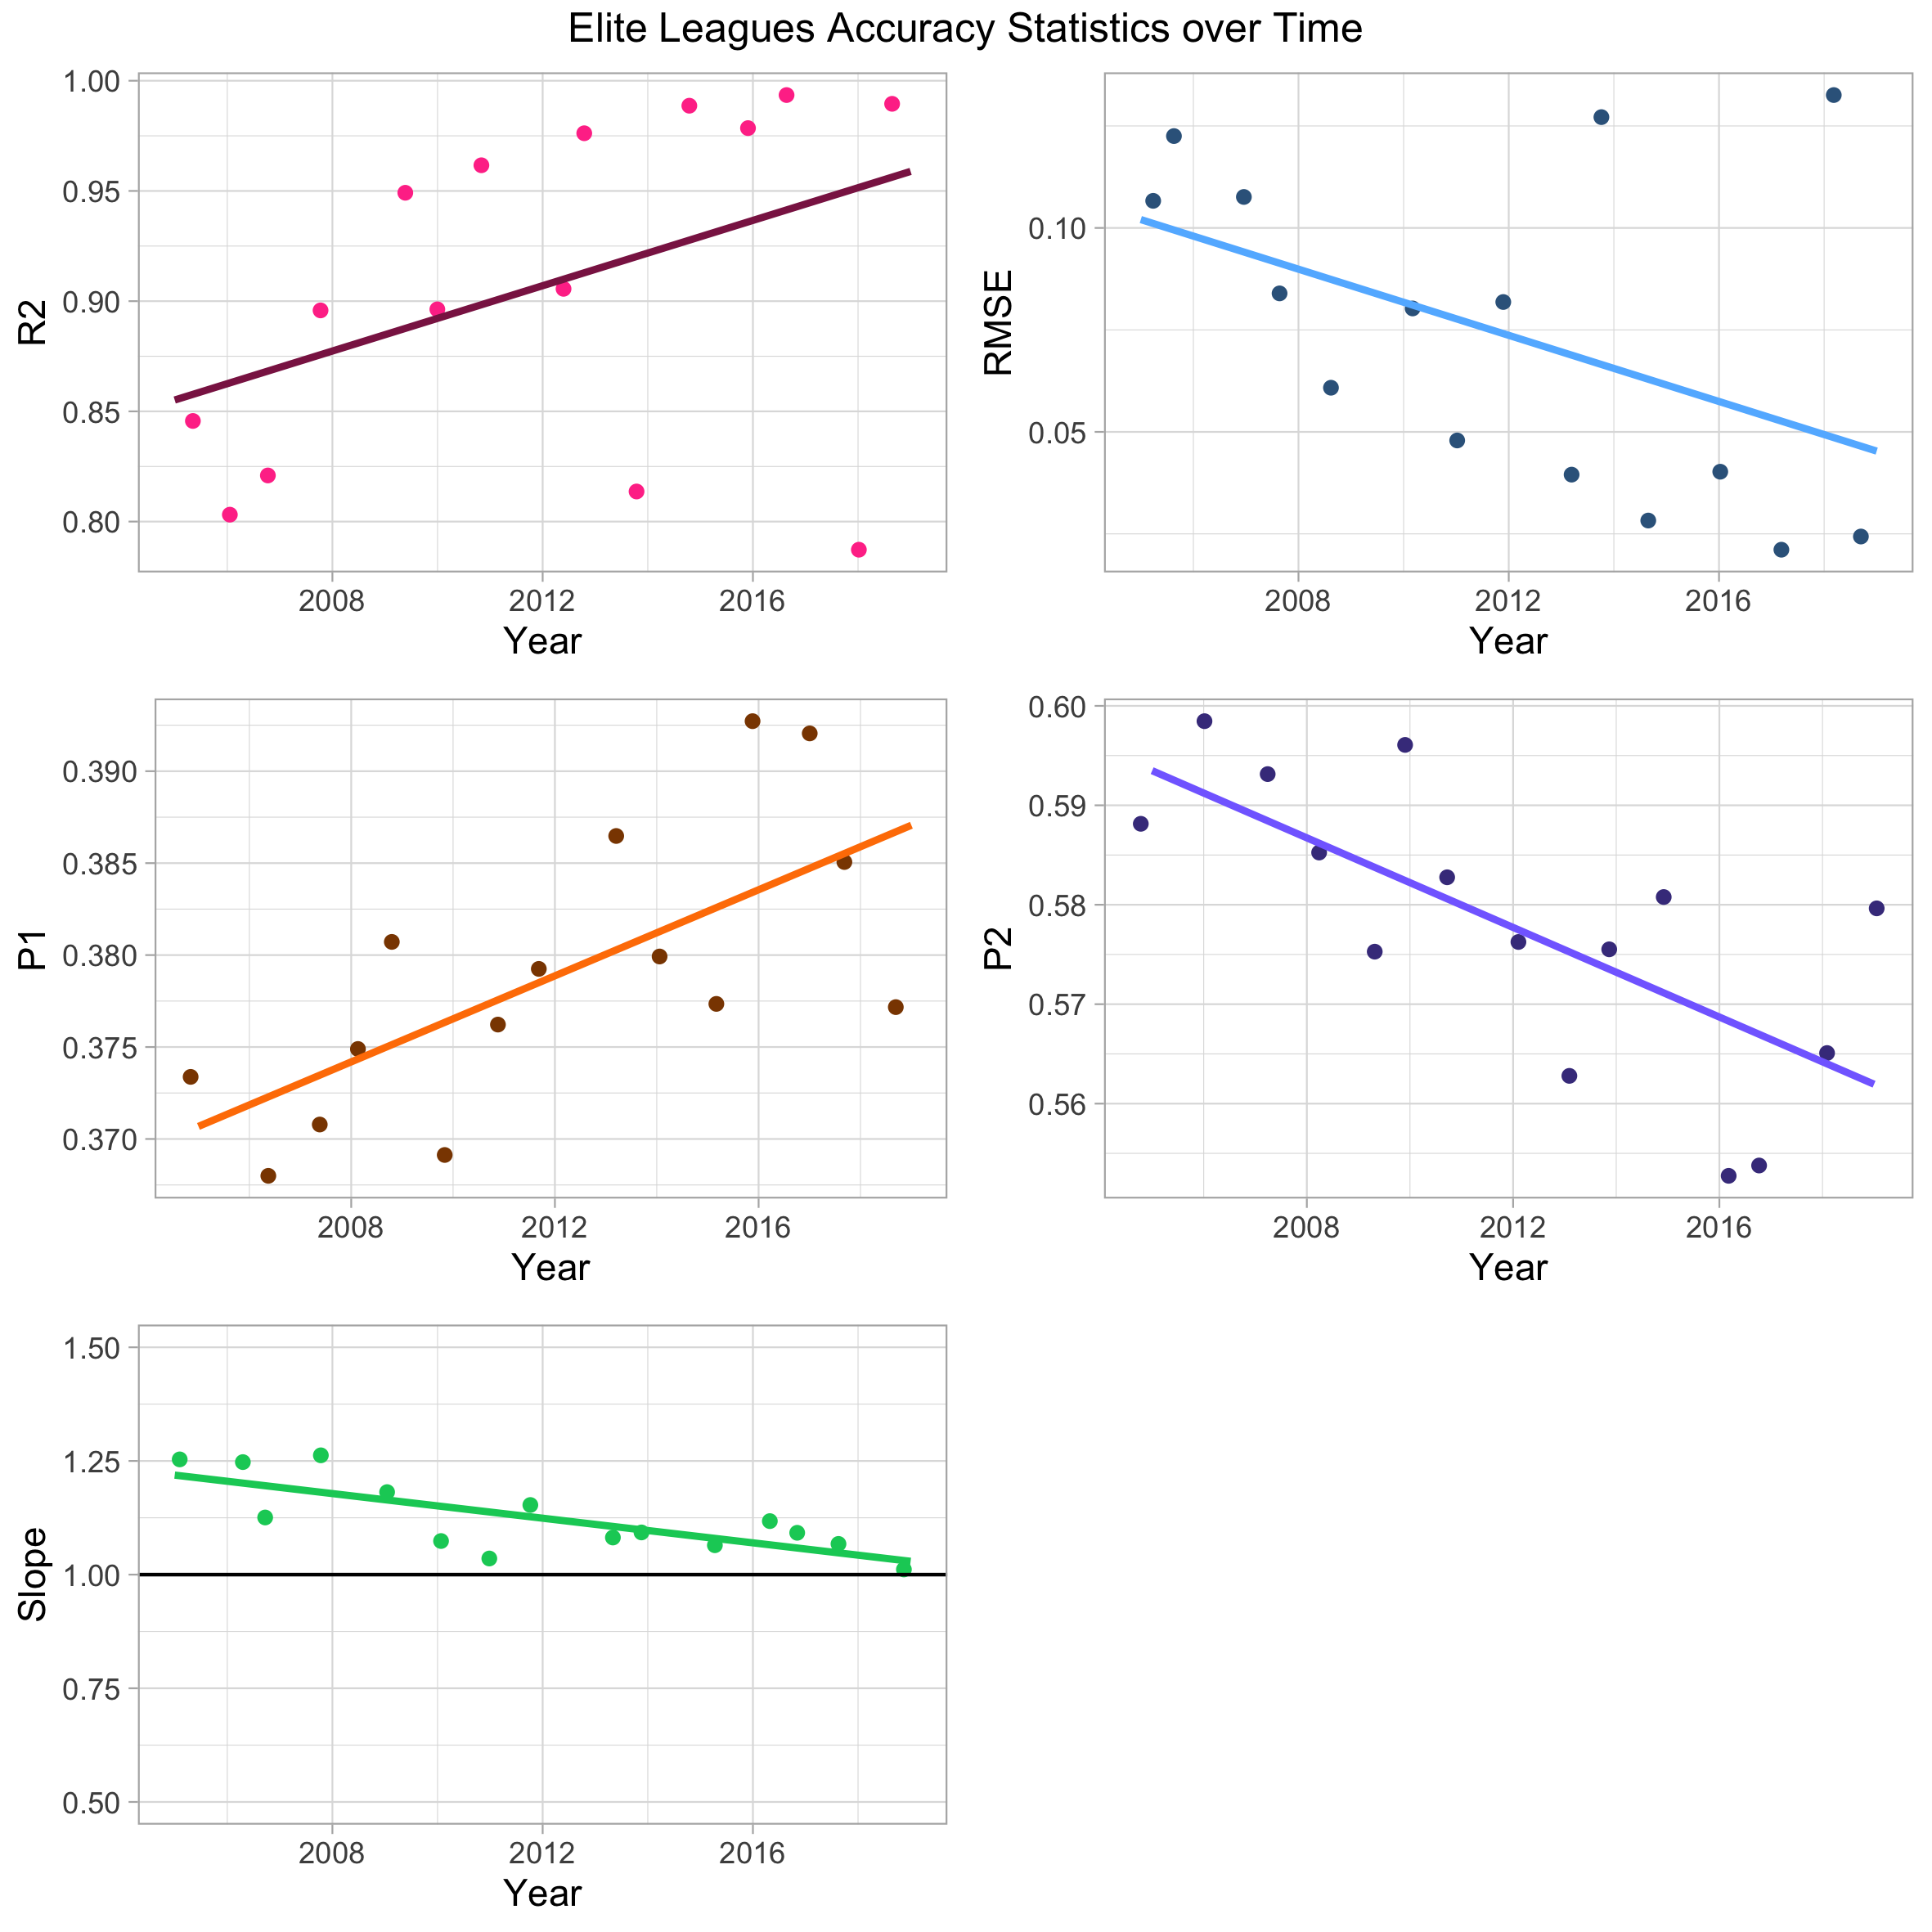
\includegraphics[width=0.75\textwidth]{elite_06_seasontimeplot.png}
	\caption{The variation of $R^2$, RMSE, $P_1$, $P_2$, and Slope over time in the \textit{elite} leagues data.}\label{FIG:01_06_seasontime}
\end{center}\end{figure}\vspace{3mm}

The figure clearly shows that accuracy is improving over time, for each measure: $R^2$ and $P_1$ are increasing; RMSE and $P_2$ are decreasing; and the Slope is approaching the ideal $y=1$ line. This is likely due to advances in the betting models used by bookmakers and increased information available, such as historical data and more metrics, \textsc{e.g.}, Expected Goals (xG) \autocite{xgoals}.

\pagebreak

\section{Principal Component Analysis}\label{sec:elitepca}
The final analysis in this chapter is a pair of principal component analyses: firstly, by-league; secondly, by-season, used to group similar observations. Principal components analysis (PCA) is a tool used in multivariate analysis to simplify the number of variables a data set has \autocite{wold87}, aiming to find `lines and planes of closest fit to systems of points in space' \autocite{pearson1901}. Graphically PCA can be thought of as setting a `new' pair of axes to a scatter plot: the `new' $x$ axis being on the \textsc{line of best fit} and the `new' $y$ axis being on the line of worst fit. 

\subsection{Choosing Which Components to Keep}
The importance of components output will show how much variation is accounted for by each component, both individually and cumulatively from the `most influential' to the `least.' In this project, two methods for choosing which components to keep are used. \textsc{n.b.}, it can be shown the eigenvalues are equal to the variances \autocite{alto19}. First, the \textit{Kaiser criterion}, which states to only keep a component if its variance (eigenvalue) is greater than 1 \autocite{kaiser74}. The choice of 1 is arbitrary and not recommended as a strict rule \autocite{fabrigar99}, thus, a second criterion: the \textit{Jolliffe criterion} is also applied: components with eigenvalues greater than 0.7 times the average eigenvalue are retained \autocite{jolliffe72}. In both screeplots in this section, the Kaiser criterion is added. 


\subsection{By-League Principal Component Analysis}\label{ssec:byleaguepca}
To conduct the first analysis---PCA by-league---three new variables are introduced: \textit{Imbalance}, \textit{Level of Attack}, and \textit{Predictive Accuracy}. This is due to the `small-$n$-large-$p$' problem,\footnote{Also referred to as `$n<<p$', `small-$N$-large-$d$' in literature.} where one has more predictors (in this case, there are eight: $R^2$, RMSE, $P_1$, $P_2$, NAMSI, $\kappa$, Gini, and the Level of Attack) than observations/samples (six leagues) \autocite{ma11}. Thus, the number of predictors needs to be reduced to achieve meaningful results, so scaled averages of predictor groups are taken.

The Imbalance (\lstinline|imbalance| in the code), found for each country $c$ using Equation~\ref{eq:imbalance}, is a scaled average of the NAMSI $N$, inverse-$\kappa$ denoted $\tau$ (the inverse is taken so high scores in all indicate higher imbalance), and Gini coefficient $G$ (these variables were explained in Section~\ref{sec:elitecompbal}) \autocite{Goossens05}.

\begin{equation}
\textrm{Imbalance}_{c} = \frac{1}{3}\bigg[
\bigg( \frac{ c_N - \mu_N }{ \sigma_N} \bigg) + 
\bigg( \frac{ c_{\tau} - \mu_{\tau} }{ \sigma_{\tau}} \bigg) + 
\bigg( \frac{ c_G - \mu_G }{ \sigma_G} \bigg)\bigg] \label{eq:imbalance}
\end{equation}

The Level of Attack LA (\lstinline|attack.league| in the code) for each country $c$ is found by Equation~\ref{eq:attack}. This is computed in R by re-reading the dataset from \url{football-data.co.uk}, as done in Section~\ref{sec:eliteeda}, instead using the \lstinline|FTHG|, \lstinline|FTAG|, \lstinline|HS| (Home Shots), and \lstinline|AS| (Away Shots) columns. For $n$ seasons of data, the Level of Attack is defined as the average ratio of shots per game (HS+AS) to goals per game (HG+AG). (\textsc{n.b.}, \url{football-data.co.uk} only has the shots data for the Portuguese Premiera Liga from the 2017/18 season onwards; it is thus assumed the Level of Attack in the league has been constant since 2005 at the level from 2017.)

\begin{equation}
\textrm{LA}_c = 
\frac{1}{n}\sum^{n}_{s=1} \bigg(\frac{\mu_{(HS+AS),\ s}}{\mu_{(HG+AG),\ s}} \bigg)\label{eq:attack}
\end{equation}

Similar to imbalance, the Predictive Accuracy PA (\lstinline|predacc| in the code) is a scaled average of the predictive variables: $R^2$, RMSE, $P_1$ and $P_2$ (the inverse of RMSE and $P_2$ is taken, denoted $\zeta$ and $\theta$ respectively), found by Equation~\ref{eq:predacc}.

\begin{equation}
\textrm{PA}_{c} = \frac{1}{4}\bigg[
\bigg( \frac{ c_{R^2} - \mu_{R^2} }{ \sigma_{R^2}} \bigg) + 
\bigg( \frac{ c_{\zeta} - \mu_{\zeta} }{ \sigma_{\zeta}} \bigg) + 
\bigg( \frac{ c_{P_1} - \mu_{P_1} }{ \sigma_{P_1}} \bigg) +
\bigg( \frac{ c_{\theta} - \mu_{\theta} }{ \sigma_{\theta}} \bigg)
\bigg] \label{eq:predacc}
\end{equation}


Once these values are computed, PCA can be ran using the code below. This results in three principal components. The output from the code is in Table~\ref{tab:leaguepcvals}, where the \textit{rotations} are the component values.

\begin{lstlisting}
pc.league <- matrix(c(imbalance, attack.league, predacc), ncol=3, byrow=F)
colnames(pc.league) <- c("imbalance", "attack", "predacc")
rownames(pc.league) <- countries

league.model <- prcomp(pc.league)
league.model$rotation; summary(league.model)
\end{lstlisting}


\begin{table}[h!]\begin{center}\begin{tabular}{c|ccc}
\multicolumn{4}{l}{\textbf{Importance of components:}}\\ \hline
Standard deviation     &1.166 &0.5301 &0.13284\\
Proportion of Variance &0.820 &0.1694 &0.01064\\
Cumulative Proportion  &0.820 &0.9894 &1.00000\\\hline\hline
\multicolumn{4}{l}{\textbf{Component rotations:}} \\
						& PC1 & PC2 & PC3  \\\hline
\lstinline|imbalance| & 0.7382378&  0.4105132& -0.5352419\\
\lstinline|attack|    &-0.3206651& -0.4845176& -0.8138898\\
\lstinline|predacc|   & 0.5934466& -0.7724776&  0.2260519\\ \hline\hline

\end{tabular}\end{center}\caption{By-League PCA values.}\label{tab:leaguepcvals}
\end{table}

\subsubsection{Component Retention}
By the both the Kaiser and Jolliffe criterions, only PC1 is retained. Figure~\ref{FIG:01_07b_seasonpca} has the Kaiser criterion overlaid; the mean variance times 0.7 is found by:
\begin{lstlisting}
> mean(c(1.166**2, 0.5301**2, 0.13284**2))*0.7
[1] 0.3869153
> 0.5301**2
[1] 0.281006
\end{lstlisting}

\begin{figure}[h!]\begin{center}
	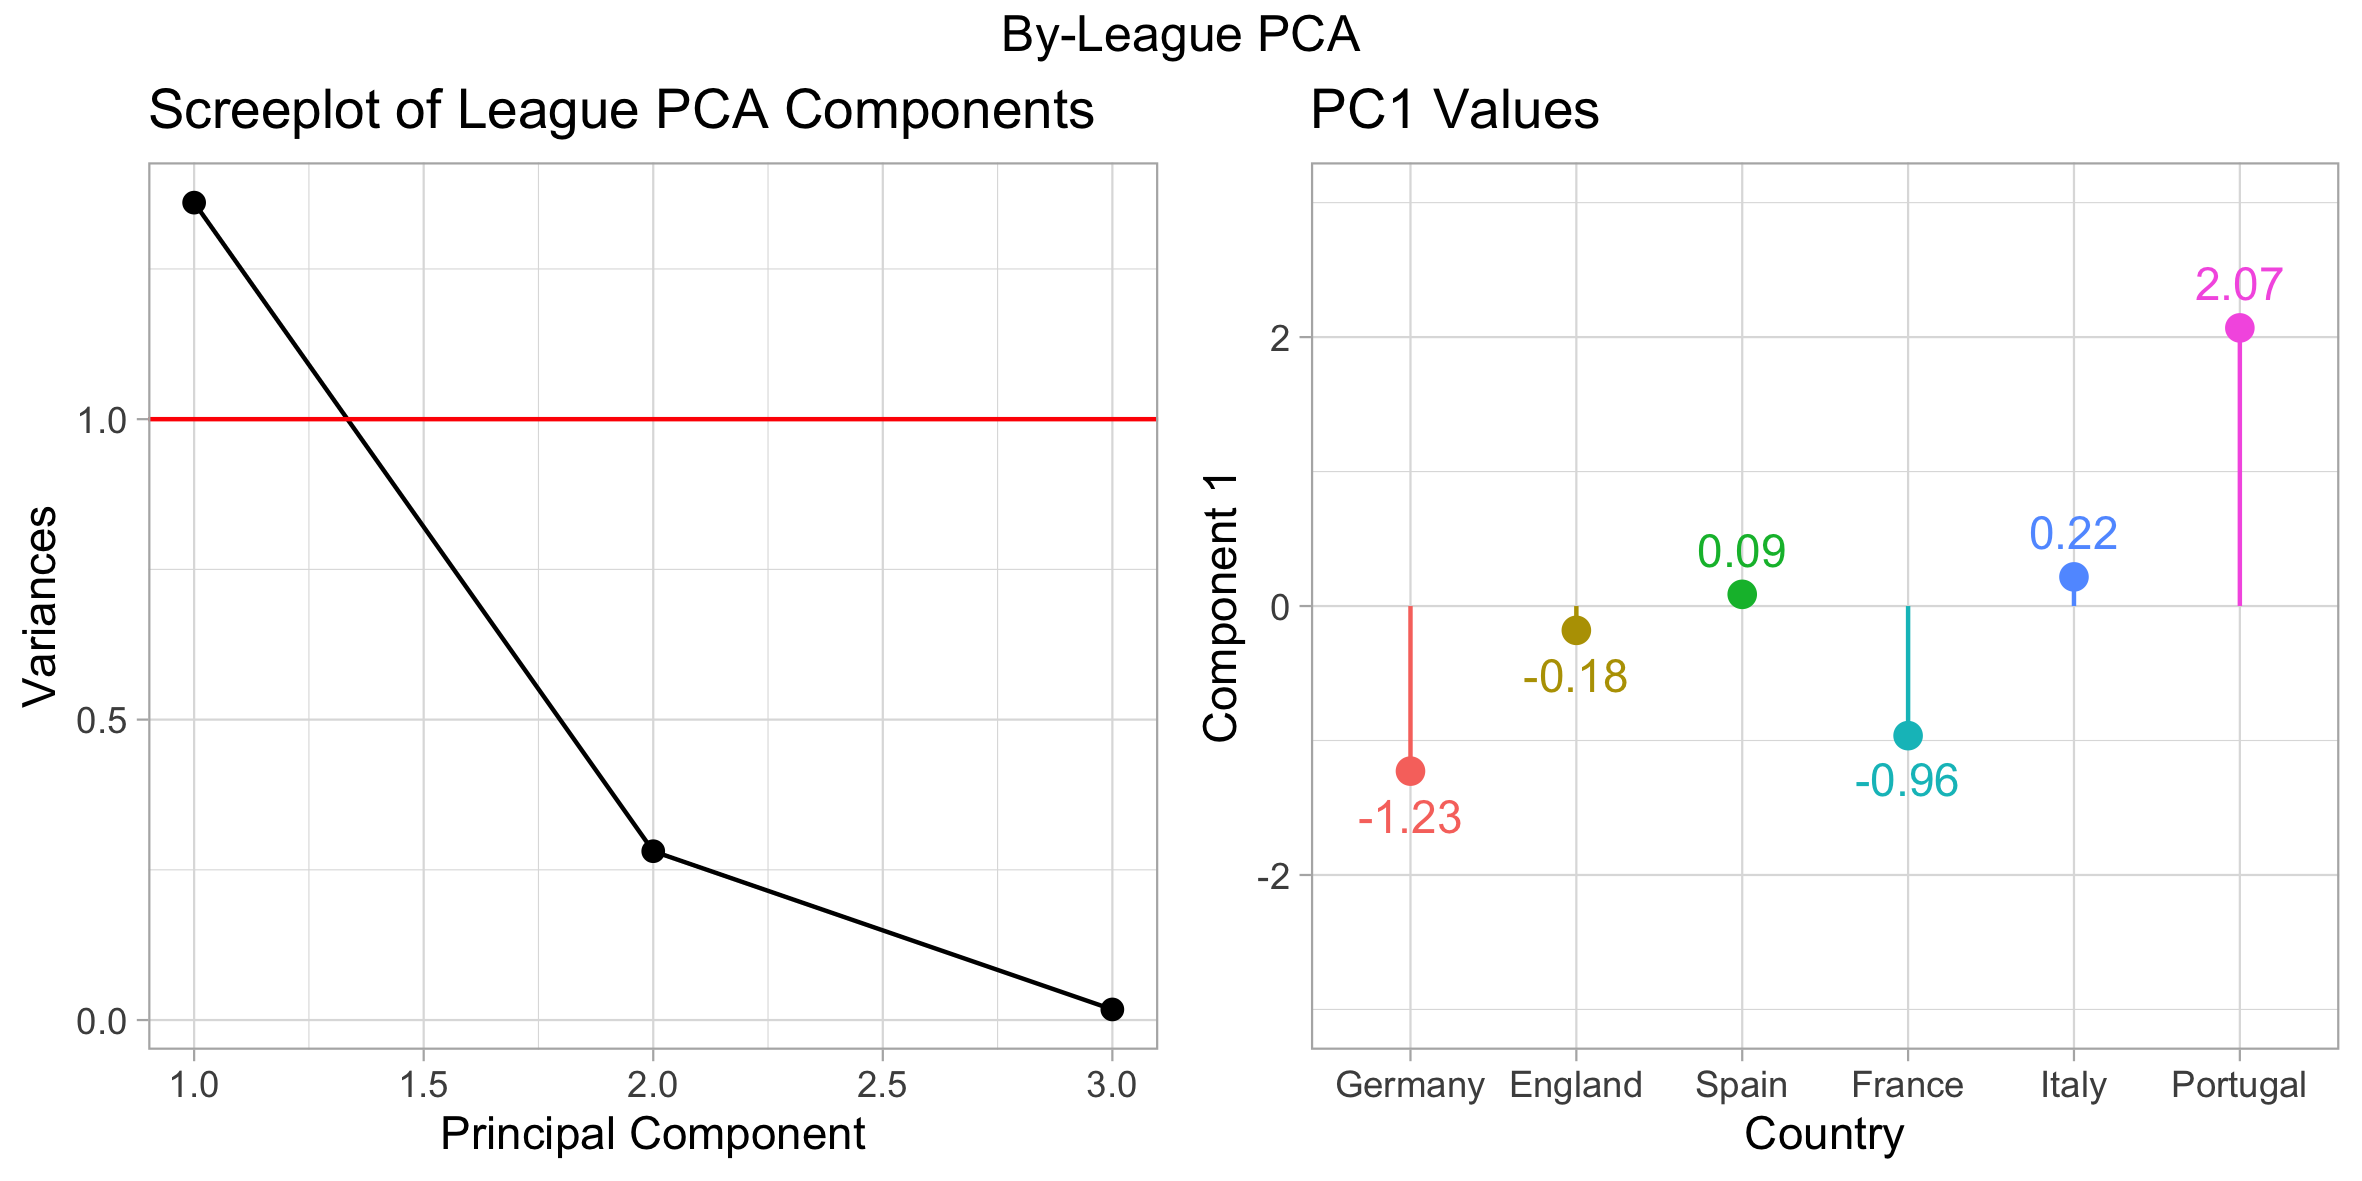
\includegraphics[width=0.8\textwidth]{elite_07a_leaguepca.png}
	\caption{By-League PCA figures.}\label{FIG:01_07_leaguepca}
\end{center}\end{figure}

\subsubsection{Interpretation}
PC1 can be considered a contrast between the Imbalance and Predictive Accuracy (PA), against the Level of Attack (LA) in a league (high values could be due to the league being defensive, or high imbalance and accuracy). A plot of the PC1 values is provided alongside the screeplot in Figure~\ref{FIG:01_07_leaguepca}.\vspace{3mm}

There are three groupings that can be made from this plot: the first, is the Portuguese league on its own, with the highest score (2.07) by far. Second are the three leagues near a score of 0, Italy (0.22), Spain (0.09), and England (-0.18). Finally, the most-negative group of leagues are the French (-0.96) and German (-1.23) leagues. This analysis appears has been dominated by the Imbalance and PA scores: literature has shown the Spanish (attacking) and Italian (defensive) leagues have opposing styles of play \autocite{bosca09}, yet have a similar PC1 value. Both leagues show similar competitive balance statistics (Table~\ref{tab:compbalcoeffs}) and accuracy statistics (Table~\ref{tab:leaguevalues}) indicating the style of play hasn't affected the PC1 score enough to provide conclusive findings. Further analysis with more methods of analysing the style of play may provide better results.

\pagebreak
\subsection{By-Season Principal Component Analysis}\label{ssec:byseasonpca}
Unlike with Section~\ref{ssec:byleaguepca}, there are more observations (15 seasons) than predictors (five: the four accuracy measures and the Level of Attack; competitive balance values are unavailable by-season), so there is no need to take scaled averages to reduce the number of predictors. Thus, PCA is conducted on the following variables: $R^2$, inverse RMSE ($\zeta$), $P_1$, inverse $P_2$ ($\theta$), and the Level of Attack LA for that season, found by Equation~\ref{eq:attackseason}, where $c$ represents the country; $s$ the season. 
\begin{equation}
\textrm{LA}_s = 
\frac{1}{n}\sum^{n}_{c=1} \bigg(\frac{\mu_{(HS+AS),\ c}}{\mu_{(HG+AG),\ c}} \bigg)\label{eq:attackseason}
\end{equation}

The code, including the creation (and scaling) of a dataframe, is below; the outputs are in Table~\ref{tab:pcaseason}, as well as a screeplot and a scatter plot of PC1 vs. PC2 in Figure~\ref{FIG:01_07b_seasonpca}.

\begin{lstlisting}
pc.season <- matrix(c(rsqu.season, (1/rmse.season), p1.season, (1/p2.season), attack.season), ncol = 5, byrow=F)
colnames(pc.season) <- c("rsqu", "inv rmse", "p1", "inv p2", "attack")
rownames(pc.season) <- seasons
pc.season.sc <- scale(pc.season)

season.model <- prcomp(pc.season.sc)
summary(season.model); round(season.model$rotation,3)
\end{lstlisting}

\begin{table}[h!]\begin{center}\begin{tabular}{c|rrrrr}
\multicolumn{6}{l}{\textbf{Importance of components:}} \\ \hline
					&PC1&    PC2&    PC3&     PC4&     PC5\\\hline
Standard deviation    & 1.8112& 0.9998& 0.7909& 0.30632& 0.02448\\
Proportion of Variance&0.6561 &0.1999& 0.1251& 0.01877& 0.00012\\
Cumulative Proportion & 0.6561 &0.8560& 0.9811& 0.99988& 1.00000\\ \hline \hline
\multicolumn{6}{l}{\textbf{Component rotations:}} \\ \hline 
&PC1    &    PC2     &   PC3   &      PC4      &    PC5\\\hline
$R^2$      &0.409& -0.624&  0.199&  0.636&  0.013\\
Inverse RMSE, $\zeta$  &0.453& -0.495& -0.241& -0.701& -0.010\\
$P_1$        &0.489&  0.364&  0.360& -0.055& -0.704\\
Inverse $P_2$, $\theta$    &0.491&  0.372&  0.333& -0.070&  0.710\\
Level of Attack   &-0.383& -0.308&  0.813& -0.310&  0.014\\
\end{tabular}\end{center}\caption{By-Season PCA values.}\label{tab:pcaseason}\end{table}

\begin{figure}[h!]\begin{center}
	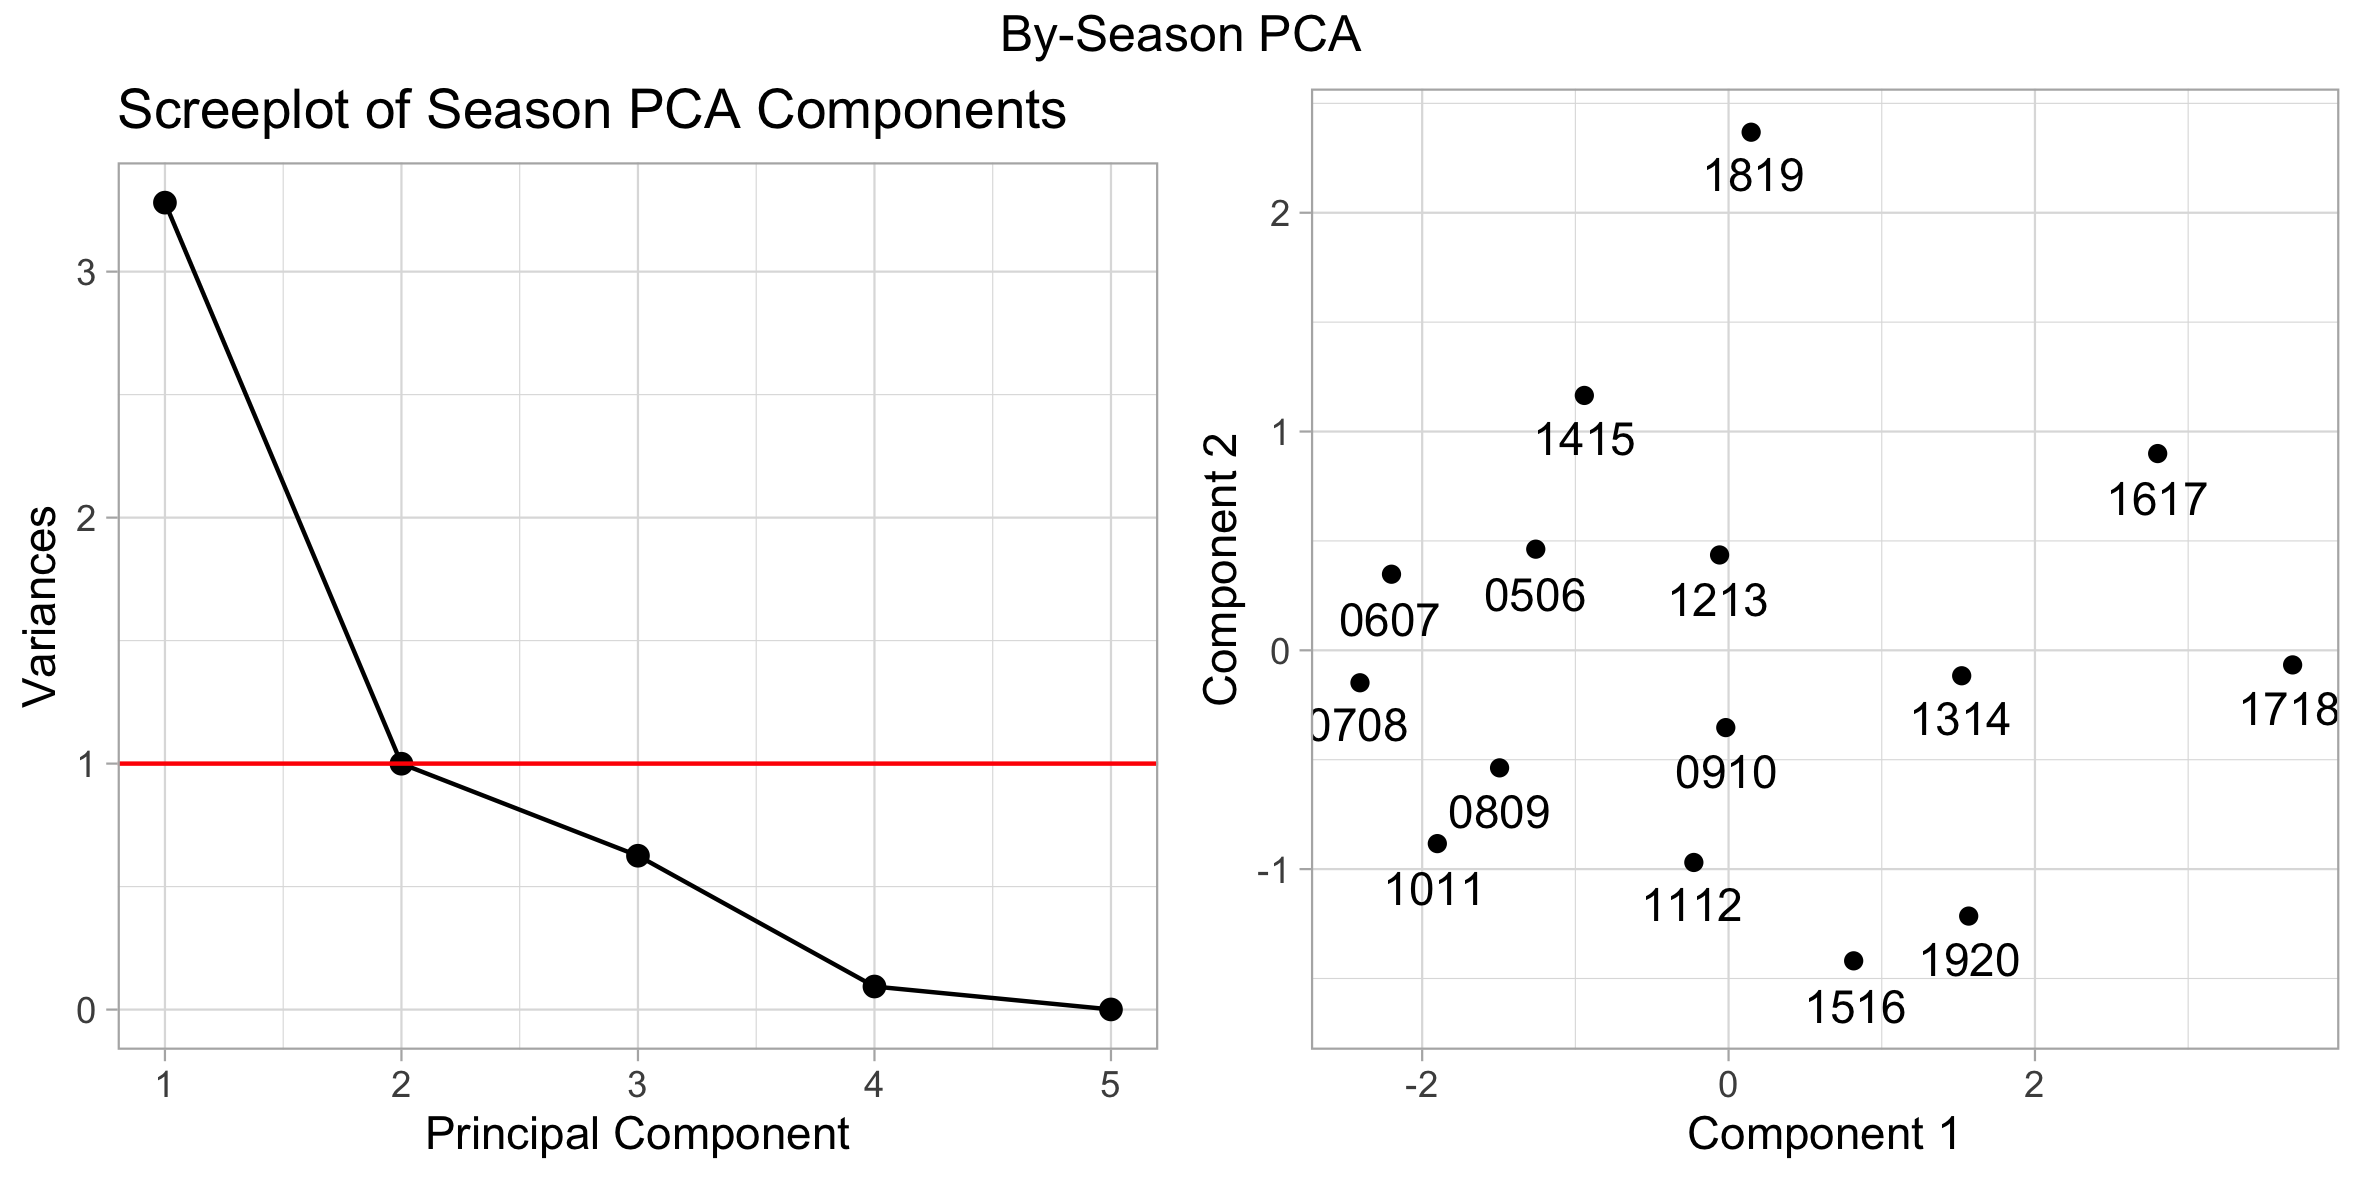
\includegraphics[width=0.8\textwidth]{elite_07b_seasonpca.png}
	\caption{By-Season PCA figures.}\label{FIG:01_07b_seasonpca}
\end{center}\end{figure}

\pagebreak

\subsubsection{Component Retention}
The importance of components output (Table~\ref{tab:pcaseason}) shows the first two components account for 85.6\% of the cumulative variance. The Kaiser criterion on the screeplot (Figure~\ref{FIG:01_07b_seasonpca}) suggests to retain PC1, and that PC2 is borderline (on the criterion line). Considering the Jolliffe criterion, it is recommended to keep both PC1 and PC2:

\begin{lstlisting}
> mean(c(1.8112**2, 0.9998**2, 0.7909**2, 0.30632**2, 0.002448**2)) * 0.7
[1] 0.6999169
> 0.9998**2 #Component 2
[1] 0.9996
> 0.7909**2 #Component 3
[1] 0.6255228
\end{lstlisting}

\subsubsection{Interpretation}
PC1 can be interpreted as a contrast between the predictive variables ($R^2$, $\zeta$, $P_1$, $\theta$), and the level of attack, with high values being awarded to seasons with high levels of accuracy, and/or lower levels of attacking football.

PC2 can be interpreted as a contrast between $P_1$ and the inverse of $P_2$, and---mainly---$R^2$. Whilst both are statistics of accuracy, the two are not mutually agreeable: in Table~\ref{tab:seasonvalues}, the 2018/19 season has the extreme poor-performing $R^2$ and RMSE, but performs on-trend for $P_1$ and $P_2$ (Figure~\ref{FIG:01_06_seasontime}). \vspace{3mm}

In the PC1 vs. PC2 plot in Figure~\ref{FIG:01_07b_seasonpca}, the earlier years (2005/06 until 2012/13) are contained within the bottom-left (low PC1, low PC2) of the graph (bounded by $x=0,\ y=0.5$); in the bottom right are the 15/16, 19/20, 13/14 and 17/18 seasons, with low PC2, and high PC1: indicating lower attacking football (high PC1), and high levels of accuracy, especially the $R^2$ and RMSE measures, indicating both a trend of accuracy increasing over time (as mentioned in Section~\ref{sec:comparingseasons}), and of more recent football seasons being more attacking. This is an area for future research, perhaps using a larger dataset and more advanced measures of attacking styles of play.

\section{Conclusion}\label{sec:eliteconclusion}
In this chapter, it has been shown that the levels of bookmaker accuracy are high in the 1X2 Home Win and Away Win markets: in each of the \textit{elite} European leagues, the coefficient of determination $R^2$ was above 95\% with the RMSE below 0.055. From the scatter plot in Figure~\ref{FIG:01_03_scatter}, the linear models for Home and Away wins have a much lower standard error (and therefore a narrower CI) than the model for Draws. This, along with the $R^2$ and RMSE for each result in Table~\ref{tab:overallrsqrmse}, indicates that whilst bookmakers enjoy high accuracy with clear results, their predictions for Draws are poor, and have large room for improvement.\vspace{3mm}

In addition, it has been shown that the accuracy is impacted by the competitive balance in each league: bookmakers perform better in countries in imbalanced leagues, such as Portugal's Primiera Liga and Italy's Serie A, than in balanced leagues, such as Germany's Bundesliga and France's Ligue Une. \vspace{3mm}

\begin{center}\noindent\rule{0.5\textwidth}{0.6pt}\end{center}

In Chapter~\ref{ch:ensco}, the accuracy of bookmaker's odds in the English \& Scottish leagues is investigated across multiple levels (rather than just the \textit{elite} leagues) and betting markets (rather than just the 1X2 market). 


\chapter[English \& Scottish Leagues, 2005--20]{Assessing the accuracy of betting odds in the English \& Scottish football league pyramids, from 2005 to 2020.}\label{ch:ensco}

In this chapter, the accuracy of betting odds across multiple levels of football leagues are assessed. This is done by using the English \& Scottish football league pyramids, with the Under/Over 2.5 Goals (UO) and Asian Handicap (AH) markets considered, in addition to the 1X2 market as in Chapter~\ref{ch:elite}. Reasons for choosing these leagues are outlined in Section~\ref{sec:bginfo}. Many of the same techniques, including conducting exploratory data analysis (EDA), correlation analysis, and assessing the predictive power will be utilised. The overround across the markets and leagues, a measure of the bookmaker commission, will also be assessed.

\section{Exploratory Data Analysis}\label{sec:enscoeda}
\subsection*{Reading and cleaning the data}
Initial data analysis, checking the data source, has already been done (Section~\ref{sec:eliteida}), and thus exploratory data analysis can be conducted immediately. Again, a \lstinline|for| loop is used to read the data directly from \url{football-data.co.uk}. \vspace{3mm}

Once the data is imported, the \lstinline|level| of the league is defined. Level 1 is defined as the English Premier League (EPL) and Championship, and the Scottish Premier League (SPL). The EPL and the SPL are the top-tier leagues in their pyramids; the Championship's average revenue per club is \euro{}33 million per club, per year (\euro{}13 million on average per year more than the SPL) \autocite{deloitte20} and so is included in this level. Level 2 is defined as the remaining fully professional leagues in the pyramids: these are the English Leagues One and Two, and the Scottish Championship. Finally, Level 3 is defined as the leagues with semi-professional sides in: the English Conference and Scottish Leagues One and Two. The Under/Over 2.5 Goals (UO) and Asian Handicap (AH) consensus odds are also read in. \vspace{3mm}

After reading in the data, and adding the \lstinline|level| using a \lstinline|for| loop, the underlying and consensus probabilities (Section~\ref{sec:proboddsgambling}) are found using the same method as in Chapter~\ref{ch:elite}. There are a couple of major mistakes in \url{football-data.co.uk}'s files with handicaps recorded, fixed below:
\begin{lstlisting}
#Rangers had a -275 goal handicap vs. East Fife; assume this meant -2.75:
ensco$HomeHandicap[ensco$HomeTeam=="Rangers" & ensco$Date=="11/01/14"] <- -2.75
#Hamilton had a 12.5 goal handicap vs. Rangers; assume this meant 1.25:
ensco$HomeHandicap[ensco$HomeTeam=="Hamilton" & ensco$Date=="25/10/08"] <- 1.25
\end{lstlisting}

\subsection*{Winning Probabilities}
The correct probability (that is, the bookmaker consensus probability of the event that occurred) is found using a set of \lstinline|for| loops: this is simple for the 1X2 market (using the \lstinline|FTR| column) and the UO market (a new column, \lstinline|TotGoals = FTHG + FTAG|, is created and assessed whether it is Under or Over 2.5), but requires more thought for the AH market. \vspace{3mm}

First, the handicapped goal difference (coded as \lstinline|gap|) between the two sides is found. Full-goal handicaps can result in a Home or Away Win, or a Draw (at which point the bet is considered void and the stake returned to the bettor \autocite{Bet365Markets}). A half-goal handicap can only result in a Home or Away win. A quarter-goal handicap (\textsc{e.g.}, $\frac{3}{4}$), however, can result in a \textit{half-win} for the bettor: half of the stake is assigned to the nearest\footnote{In a number-line sense} half-handicap (in the case of $\frac{3}{4}$, this is $\frac{1}{2}$), and half to the nearest integer (1). If only one bet wins, the bettor wins on half their stake. The R code below is used for this step.

\begin{lstlisting}
ensco$ah.gap <- with(ensco, FTHG.ah - FTAG); ensco$ah.res <- NULL
for (n in 1:N){
	if (ensco$ah.gap[n]<(-0.25)){ensco$ah.res[n]<-"aw"}
	else if (ensco$ah.gap[n]==(-0.25)){ensco$ah.res[n]<-"hfaw"}
	else if (ensco$ah.gap[n]==0){ensco$ah.res[n]<-"vo"}
	else if (ensco$ah.gap[n]==0.25){ensco$ah.res[n]<-"hfhm"}
	else if (ensco$ah.gap[n]>0.25){ensco$ah.res[n]<-"hm"}
	else{}
}
\end{lstlisting}

\subsection*{Basic Calculations}
The first step, as with Section~\ref{sec:eliteeda}, is to compute the bookmaker mean probabilities for each outcome, and their corresponding standard deviations, and compare against the observed probabilities. These are shown in Table~\ref{tab:edaenscocalcs}, split by level.

\begin{table}[h!]\begin{center}\begin{tabular}[h!]{l||c|c|c}
\textbf{1X2 Market}& \textit{Level 1}& \textit{Level 2}& \textit{Level 3} \\ \hline
Mean $\mathbb{P}_{\textrm{cons}}$(Home Win) & 0.4366 & 0.4257 & 0.4292 \\ 
Observed Probability of a Home Win 			& 0.4438 & 0.4256 & 0.4352 \\ \hdashline
Standard Deviation (Home Win 1x2)			& 0.1507 & 0.1044 & 0.1238 \\ \hline

Mean $\mathbb{P}_{\textrm{cons}}$(Draw)	 	& 0.2644 & 0.2725 & 0.2613 \\ 
Observed Probability of a Draw	 			& 0.2607 & 0.2695 & 0.2406 \\ \hdashline
Standard Deviation (Draw 1x2)				& 0.0369 & 0.0195 & 0.0243 \\ \hline

Mean $\mathbb{P}_{\textrm{cons}}$(Away Win) & 0.2990 & 0.3018 & 0.3095 \\ 
Observed Probability of a Away Win	 		& 0.2955 & 0.3049 & 0.3242 \\ \hdashline
Standard Deviation (Away Win 1x2)			& 0.1366 & 0.0952 & 0.1139 \\ \hline \hline

\multicolumn{4}{l}{ } \\\hline
\textbf{Under/Over 2.5 Goals Market}& \textit{Level 1}&\textit{Level 2}& \textit{Level 3} \\ \hline
Mean $\mathbb{P}_{\textrm{cons}}$(Under 2.5 Goals)	& 0.5080 & 0.5121 & 0.4756 \\
Observed Probability of Under 2.5 Goals		& 0.5051 & 0.5184 & 0.4755 \\\hline
Mean $\mathbb{P}_{\textrm{cons}}$(Over 2.5 Goals)		& 0.4920 & 0.4879 & 0.5244 \\
Observed Probability of Over 2.5 Goals			& 0.4949 & 0.4816 & 0.5245 \\ \hdashline
Standard Deviation (Under/Over Market)		& 0.0568 & 0.0380 & 0.0504 \\ \hline \hline

\multicolumn{4}{l}{ } \\\hline
\textbf{Asian Handicap Market}& \textit{Level 1}& \textit{Level 2}& \textit{Level 3} \\ \hline
Mean $\mathbb{P}_{\textrm{cons}}$(AH Home Win)  & 0.5109 & 0.5046 & 0.5015 \\
Observed Probability of a Home Win (AH)			& 0.4011 & 0.4005 & 0.4000 \\
Observed Probability of a Half-Home Win (AH)	& 0.0434 & 0.0513 & 0.0583 \\ \hline
Mean $\mathbb{P}_{\textrm{cons}}$(AH Away Win)  & 0.4891 & 0.4954 & 0.4985\\
Observed Probability of an Away Win (AH)		& 0.3779 & 0.3920 & 0.4087 \\
Observed Probability of a Half-Away Win (AH)	& 0.0620 & 0.0741 & 0.0659 \\ \hline
Observed Probability of a Bet Being Voided 		& 0.1157 & 0.0821 & 0.0671 \\ \hdashline
Standard Deviation (Asian Handicap Market)		& 0.0678 & 0.0524 & 0.046
\end{tabular}\end{center} \caption{Basic calculations for the entire English \& Scottish data, forming part of the exploratory data analysis.} \label{tab:edaenscocalcs}\end{table}

To initially analyse this table, the 1X2 market is considered. as in Chapter~\ref{ch:elite}, the standard deviation---for all levels---is far lower for Draws than for either Home or Away Wins, indicating a consistent lack of variation in the odds offered for Draws. In addition, the standard deviations for all three outcomes are lowest for Level 2 (rather than Level 3, as one would expect, due to the amount of, or lack thereof, information available at lower levels). For all three outcomes, across all three levels, the consensus probability is remarkably close to the observed probability; the clearest examples of this are the Level 2 Home Win probabilities: 0.4257 (consensus) and 0.4256 (observed), and the Level 1 Away Win probabilities: 0.2990 (consensus) and 0.2955 (observed). \vspace{3mm}

For the UO and AH markets, bookmakers offer only two options, and thus, the standard deviations are equal for each outcome. For the UO market, the standard deviations are low (especially in Level 2, where $\sigma = 0.0380$); and the consensus and observed probabilities are very close together. In Level 3, the consensus and observed differ by 0.0001. The mean number of goals across all matches in the dataset is 2.66, so it is no surprise the means are around 0.5: it is likely the bookmakers know the mean number of goals in each level (or league), and set their odds accordingly. \vspace{3mm}

Lastly, the AH market is considered. The numbers aren't as easy to infer across due to the half-wins and voided bets: of the full Home and Away Wins, 50.57\% were Home Wins: by level, the proportions of full Home Wins are 0.5149, 0.5054 and 0.4946 for Levels 1, 2, and 3 respectively. Again, these are all remarkably close to the bookmaker consensus means. It is, as with the UO market, unsurprising these values are near 0.5: the AH market is designed to give a handicap in favour of the poorer side in the form of a goal deficit to the Home side \autocite{constantinou20}. 

\subsection*{Visual Analysis}
For visualisation of these values, several plots are produced. First are density plots, shown in Figure~\ref{FIG:02_01_densityplots}. \vspace{3mm}

The densities of each outcome in the 1X2 market reflect similar distributions as in Figure~\ref{FIG:01_02_edadensall}. The Home Win curve is symmetrically distributed about the mean, located just above 0.4; the Away Win curve has a positive skew, with the mode between 0.25 and 0.3; and the Draw curve has a negative skew with a sharp drop after the mode, at roughly 0.27, with very little overall variance. 

As expected, due to the nature of both markets, the UO and AH curves have little variation, with the mean for all four curves located at, or close to, 0.5. As both markets have two outcomes, the two curves for each market are reflections \autocite{reflection}. The last observation from these plots is the positive skew (and corresponding negative skew) of the Over 2.5 Goals curve (Under 2.5 Goals curve), suggesting the most common consensus probabilities have a slightly higher probability of Under 2.5 Goals, than Over.\vspace{3mm}

\begin{figure}[h!]\begin{center}
	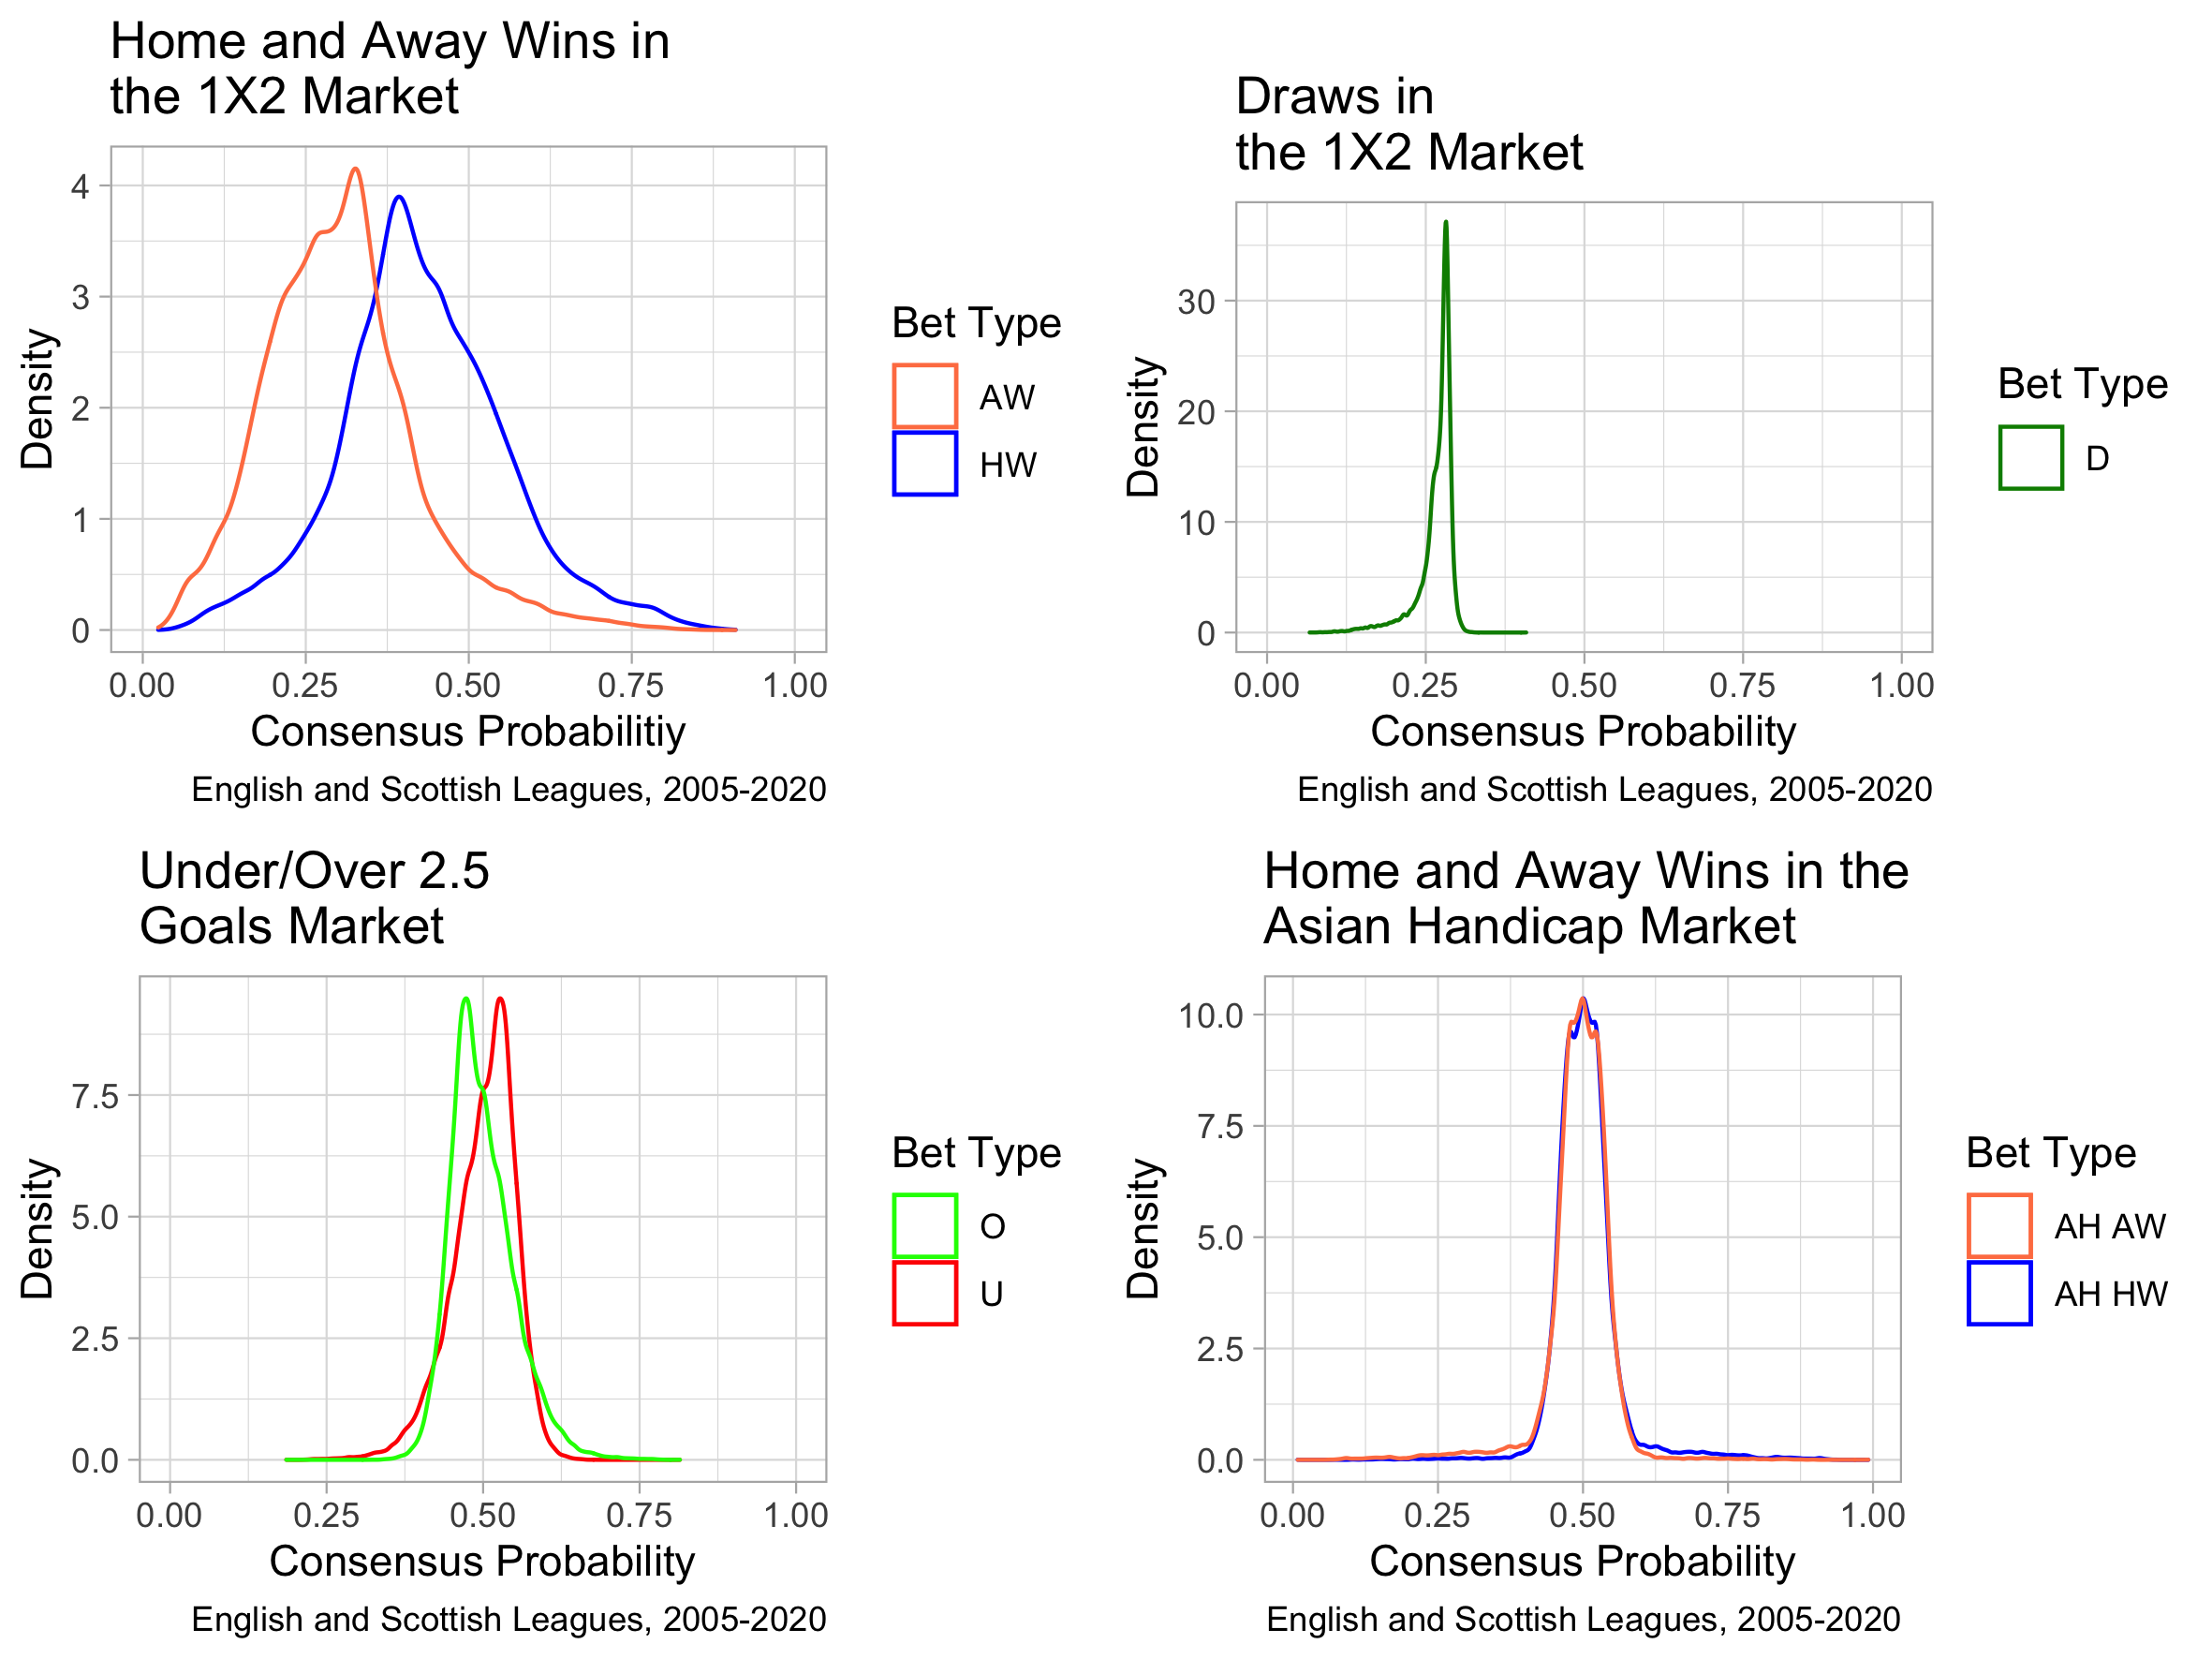
\includegraphics[width=0.9\textwidth]{ensco_04A_densities.png}
	\caption{Density plots of the consensus probabilities offered in the 1X2, UO, and AH markets.}\label{FIG:02_01_densityplots}
\end{center}\end{figure}

To assess the handicaps offered by bookmakers, two plots are created. The first, Figure~\ref{FIG:02_02a_handicap_hprob}: the handicap offered vs. consensus probability of a Home Win in the 1X2 market, with each data point grouped by level; and the second, Figure~\ref{FIG:02_02b_handicap_1x2}: the handicap offered vs. consensus probability of both a Home and Away Win in the 1X2 market. These plots are used to ensure the bookmakers handicap is consistent with the consensus probabilities of a Home or Away Win without a handicap (the 1X2 market).

Both figures show that a team with a high consensus probability of a win, whether they are the Home or Away side, have a detrimental handicap: as expected. There are a number of outliers, perhaps due to errors made by \url{football-data.co.uk}, or by random chance. % Non linear shape?

There appears to be no difference in the handicap distribution between levels.

The non-linear shape may be due to small sample sizes (shown by the data points being reduced in size), with few matches at either extreme. In addition, across all levels, there are a number of matches with a 0 handicap, despite some of these matches being highly in favour of one side. This may be due to the data being unavailable, such as the Asian Handicap market being closed for that particular match.\vspace{3mm}

\begin{figure}[h!]\begin{center}
		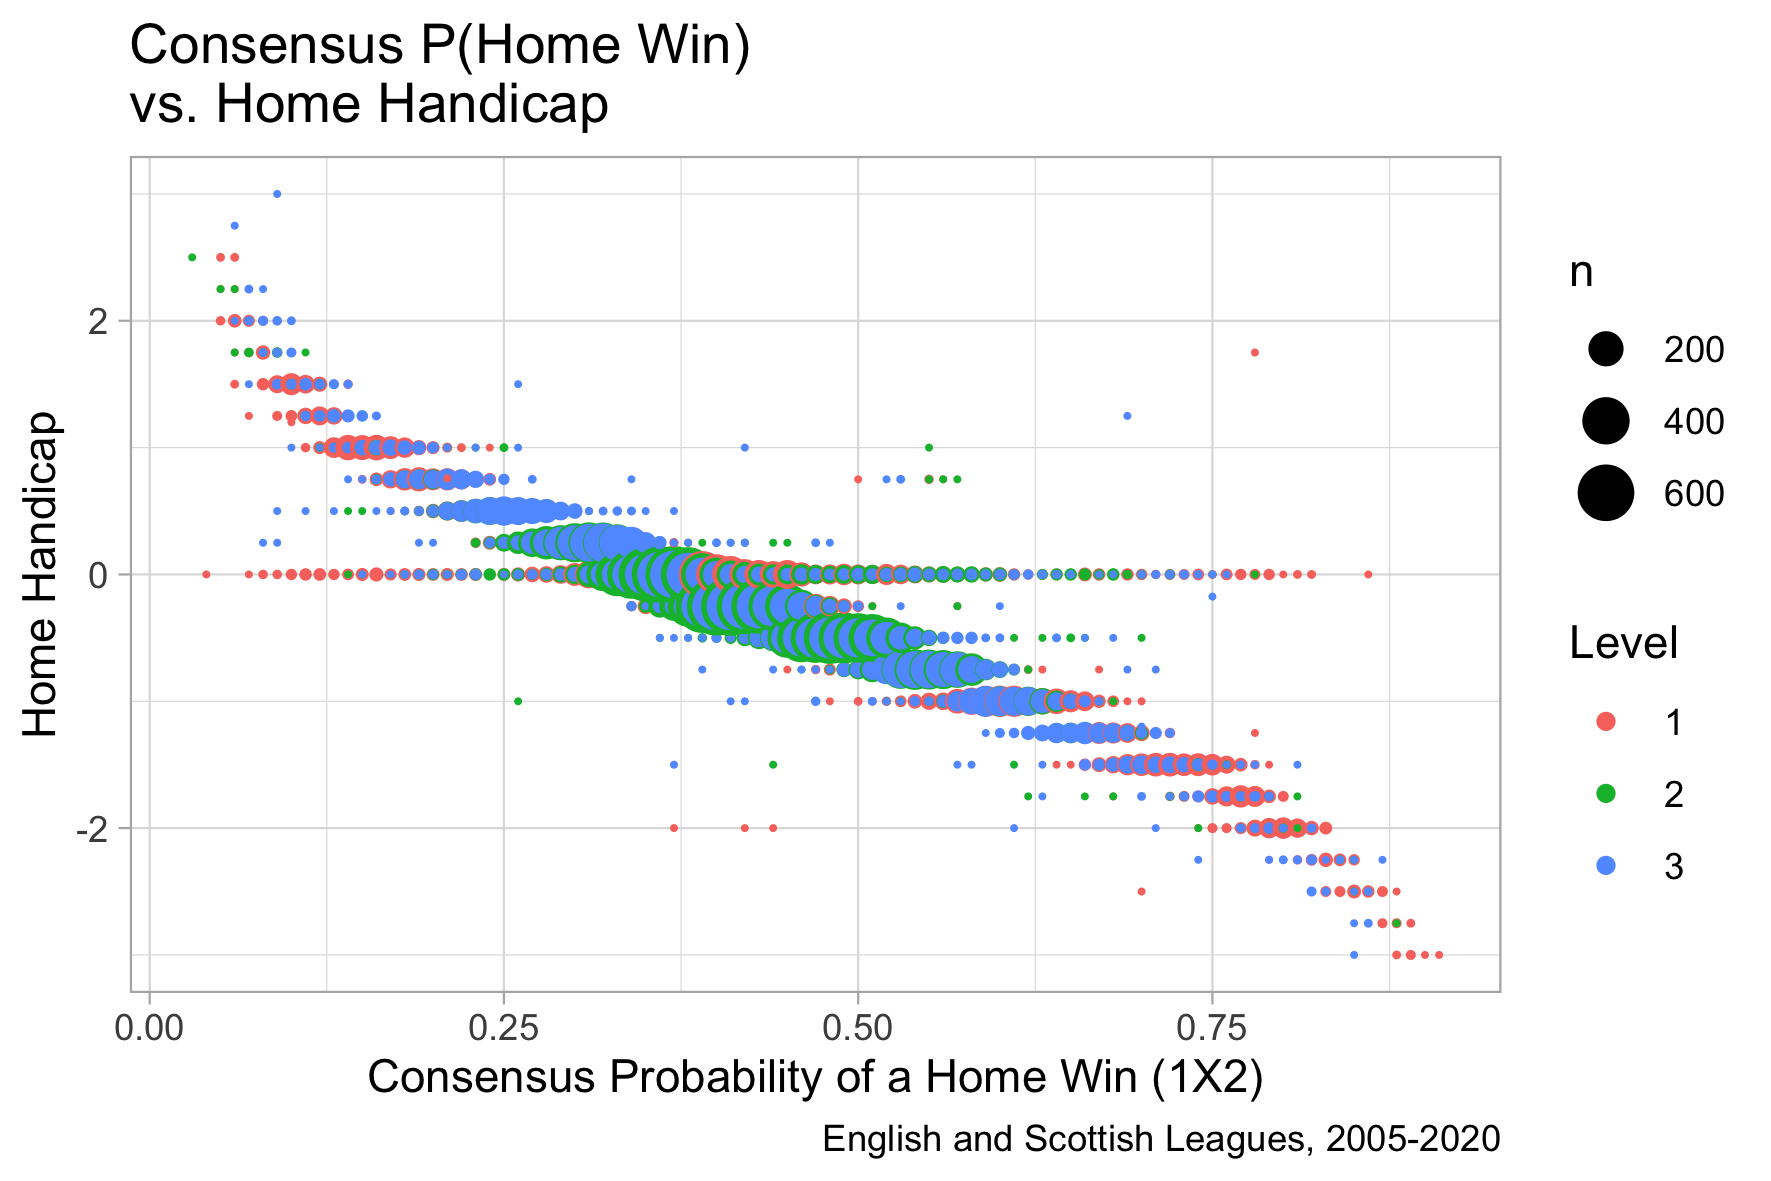
\includegraphics[width=0.75\textwidth]{ensco_05_hprob_v_hcap.png}
		\caption{The AH handicap vs. the consensus probability of a Home Win, split by level.}\label{FIG:02_02a_handicap_hprob}
\end{center}\end{figure}
\begin{figure}[h!]\begin{center}
		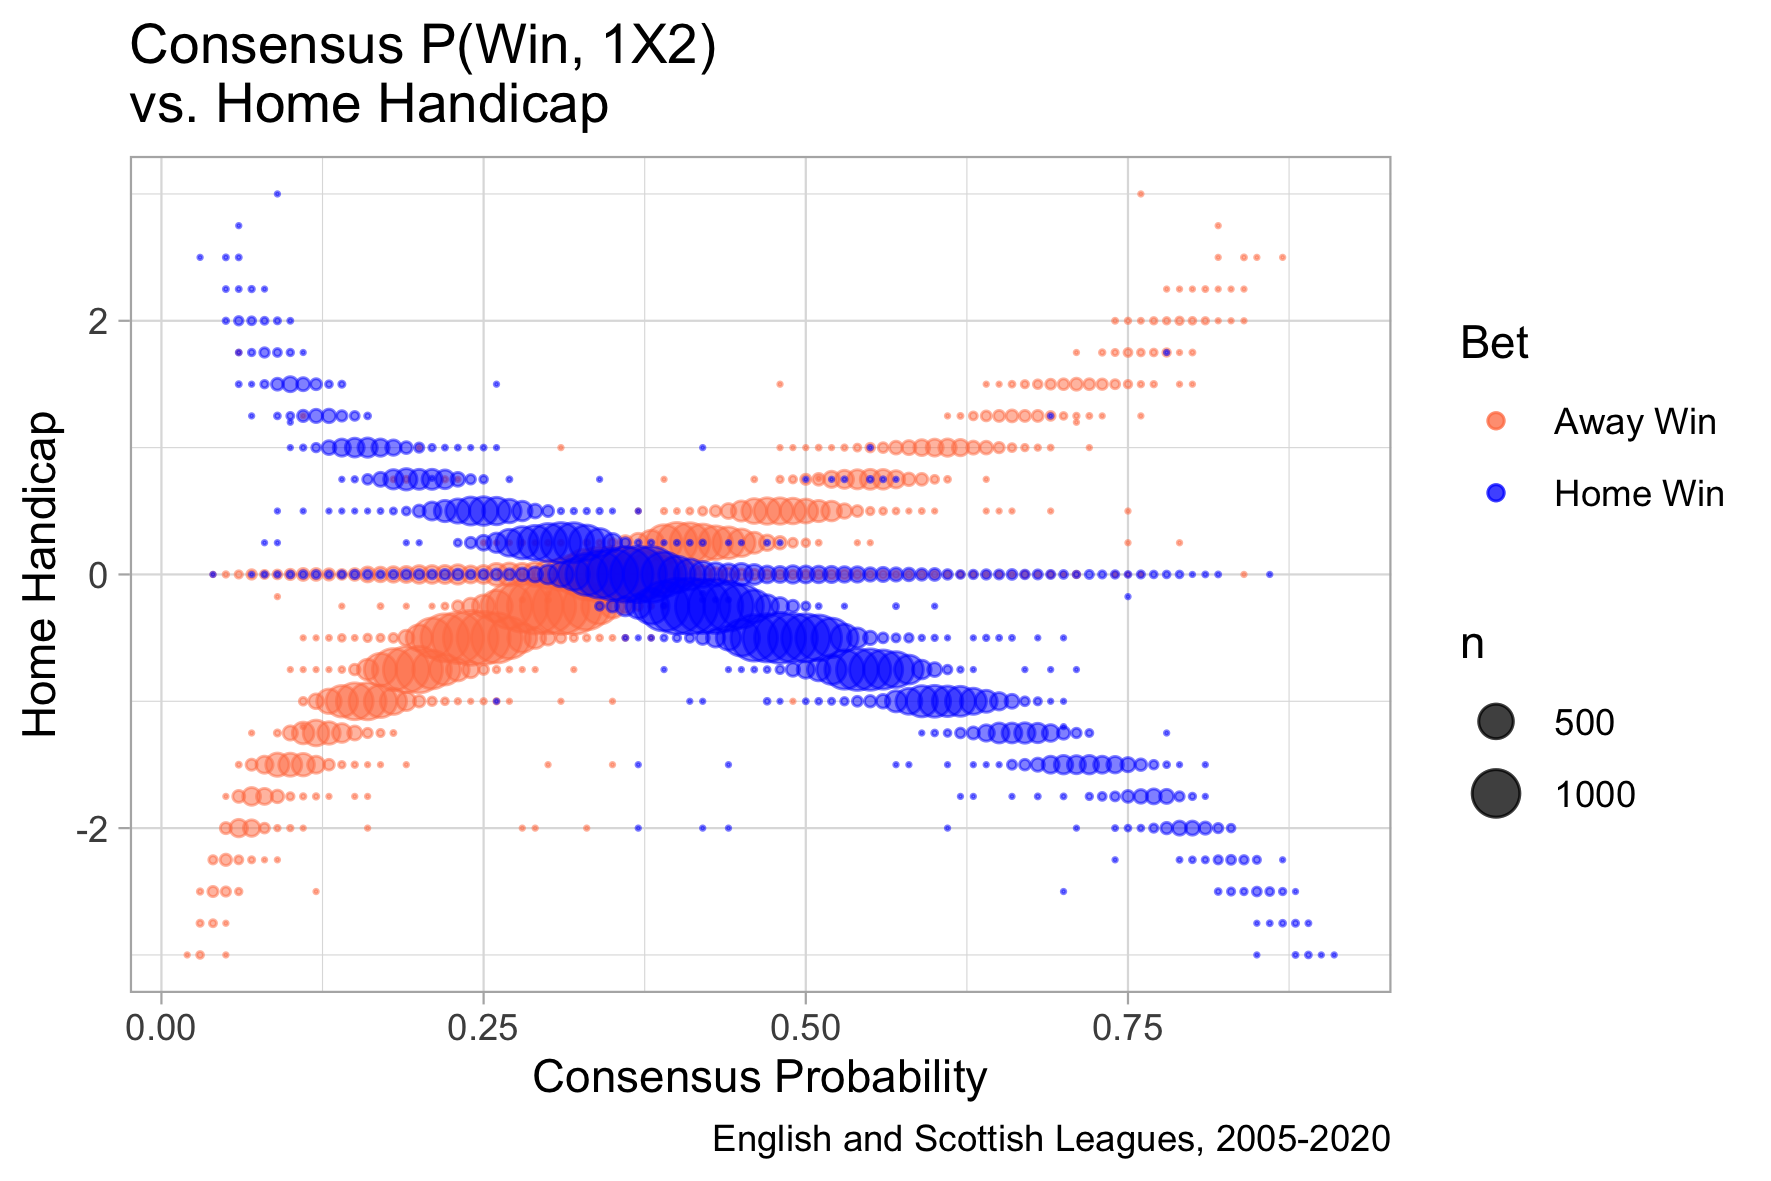
\includegraphics[width=0.75\textwidth]{ensco_05a_1x2_v_hcap.png}
		\caption{The AH handicap vs. the consensus probabilities of both a Home Win and Away Win.}\label{FIG:02_02b_handicap_1x2}
\end{center}\end{figure}

Also created are tile plots, as shown before (Section~\ref{sec:eliteeda}, Figure~\ref{FIG:01_05_tile}). This is to see if the correct consensus probabilities are greater for more \textit{convincing} wins, with both the 1X2 and UO markets considered. The bin size for each tile in both plots is given in Table~\ref{tab:enscotilebinsizes}.\footnote{The highest scoring Draw in the data for this chapter was 6--6, between Motherwell and Hibernian (05/05/2010) in the Scottish Premiership. 6+ goals is therefore chosen as the upper bound.}

Figure~\ref{FIG:02_03a_tile_1x2}, the tile plot for the 1X2 market, implies the expected result: more convincing results have a higher correct probability. The highest scoring tiles are highly-convincing Away Wins (0--5, 1--5, 2--5, 1--6+ and 0--3 are five examples of the most noticeable such tiles) and highly-convincing Home Wins (6+--0, 3--0 and 5--2), though the former is clearer. It is hard to draw meaningful conclusions from the highest scoring matches (the top right of the plot) due to low bin sizes, but at the bottom left (lowest scoring matches, where the number of matches per bin is high), the pattern holds well. 

In Figure~\ref{FIG:02_03b_tile_uo}, the tile plot for the UO market, a different \lstinline|ggplot2| palette is chosen, due to the low levels of variation in the market, and a black line is added at 2.5 Goals: the nine tiles within this bound (bottom left) contain Under 2.5 Goals; tiles outside contain Over 2.5 Goals. The `redder' tiles are those with the highest consensus probability of Over 2.5 Goals\footnote{The highest correct consensus probability, although all such tiles lie within the Over 2.5 Goals region.} (1--5, 6+--1 and 0--3, with bin sizes $n_{1-5} = 133$, $n_{6+-1}=119$ and $n_{0-3}=1085$); `bluer' tiles are those with the lowest consensus probability of Over 2.5 Goals. The 5--3 Home Win tile ($n_{5-3} = 47$) has the lowest correct probability, at around 0.4, despite eight goals being scored in these matches. Other high-scoring tiles with low correct probabilities include the 1--4, 2--6+, and 6+--6+. Each of these has a low number of matches, $n_{1-4} = 446$, $n_{2-6+} = 16$, $n_{6+-6+} = 1$. The most striking conclusion this tile plot gives, however, is the \textit{lack} of a pattern: there is no obvious feature, suggesting---as with the Draws in the 1X2 market---bookmakers struggle at placing reliable odds in the UO market.

\begin{table}[h!]\begin{center}\begin{tabular}[h!]{cc|ccccccc}
			\parbox[t]{2mm}{\multirow{7}{*}{\rotatebox[origin=c]{90}{Away Goals}}}
			&	6+ 	&   48&   38&   16&   12 &   1 &  1  &1 \\
			&	5 	&  115&  133&   74&   23 &  18 &  6  &---\\
			&	4 	&  407&  446&  268&  144 &  54 & 19  &5 \\
			&	3	& 1085& 1337& 1003&  508 & 167 & 47  &7 \\
			&	2	& 2388& 3530& 2628& 1242 & 411 &125  &44\\
			&	1	& 4091& 6012& 4372& 1993 & 763 &245  &119\\
			&	0	& 3590& 5009& 3761& 1954 & 782 &304  &132\\ \hline	
			&		&  0 	& 1 	& 2 	& 3 	& 4 	& 5		& 6+\\
			&\multicolumn{7}{c}{Home Goals}  	
\end{tabular}\end{center}\caption{The bin size for each tile of Figures~\ref{FIG:02_03a_tile_1x2} and \ref{FIG:02_03b_tile_uo}.}\label{tab:enscotilebinsizes}
\end{table}
\begin{figure}[h!]\begin{center}
		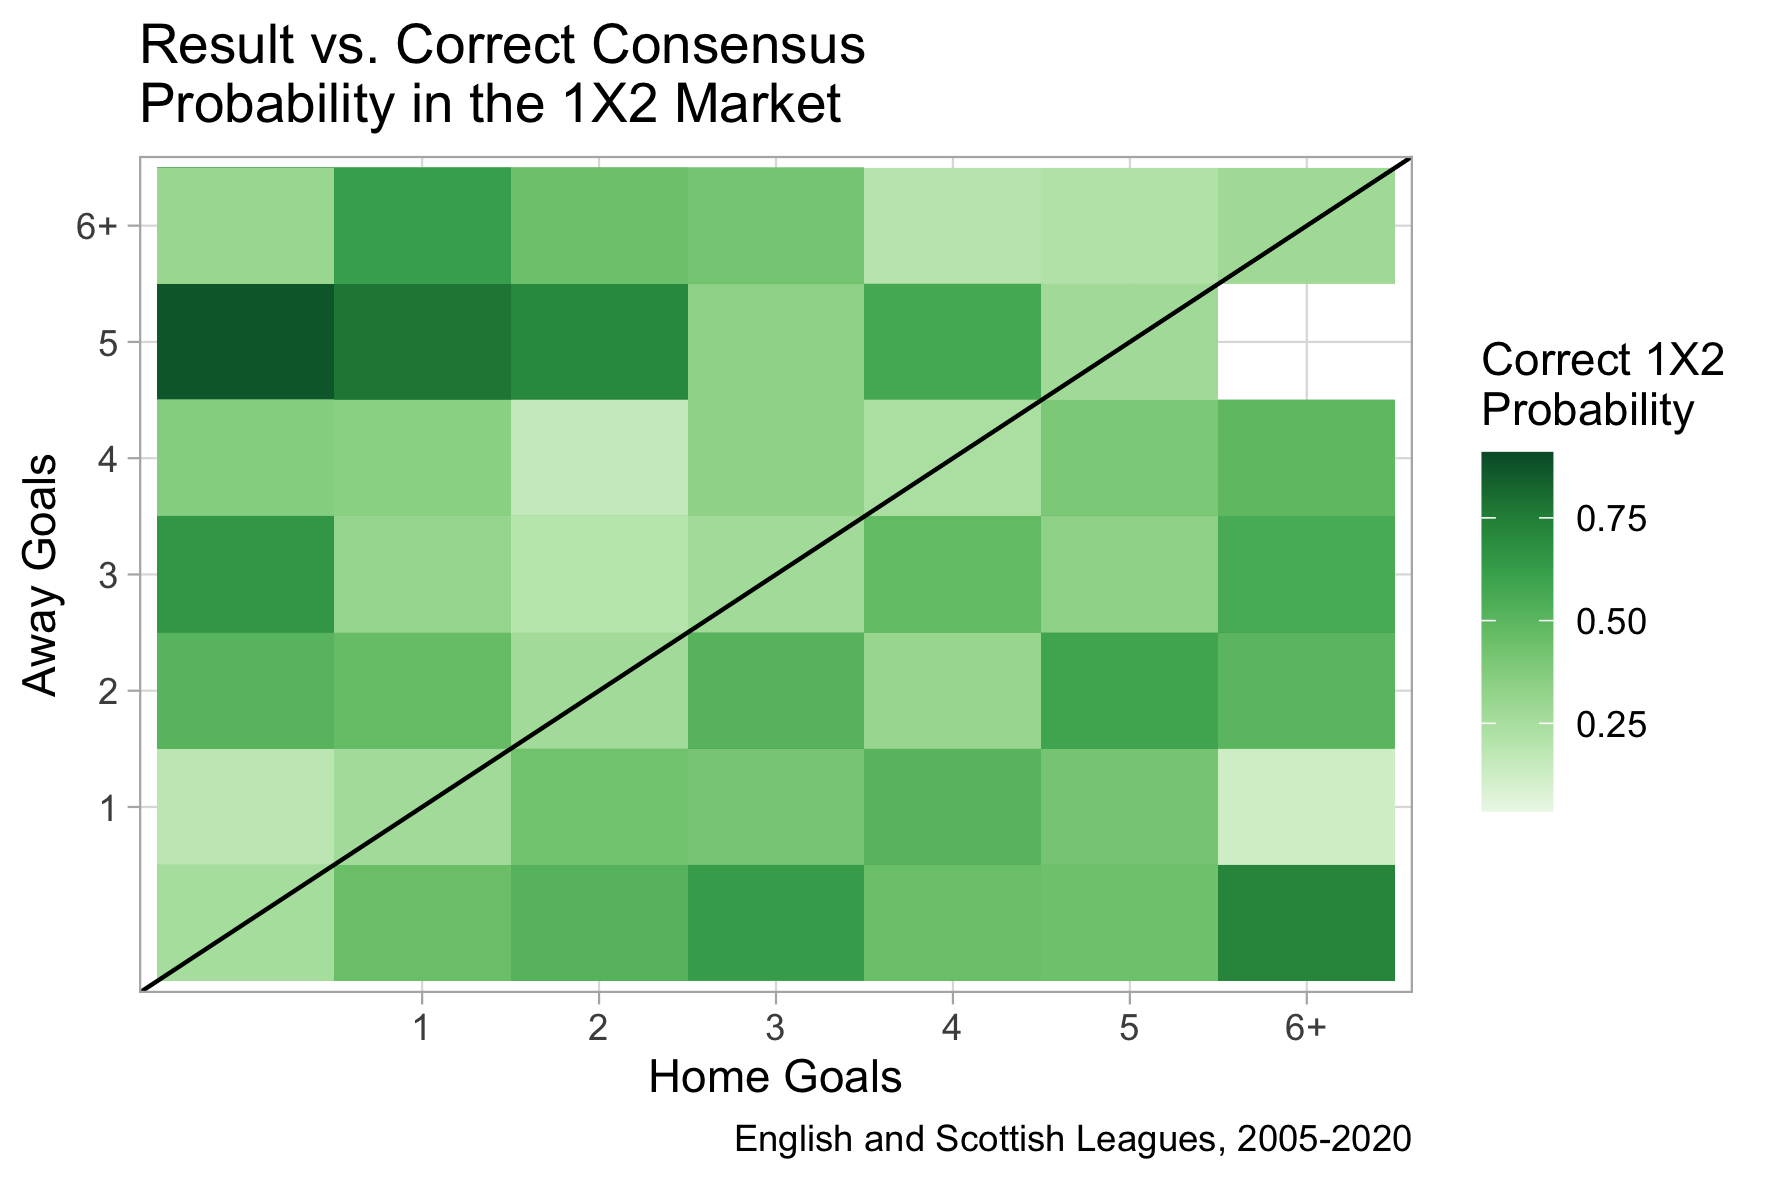
\includegraphics[width=0.7\textwidth]{ensco_06_tile_1x2.png}
		\caption{Tile plot of the correct 1X2 probability vs. the full-time result.}\label{FIG:02_03a_tile_1x2} 
\end{center}\end{figure}
\begin{figure}[h!]\begin{center}
		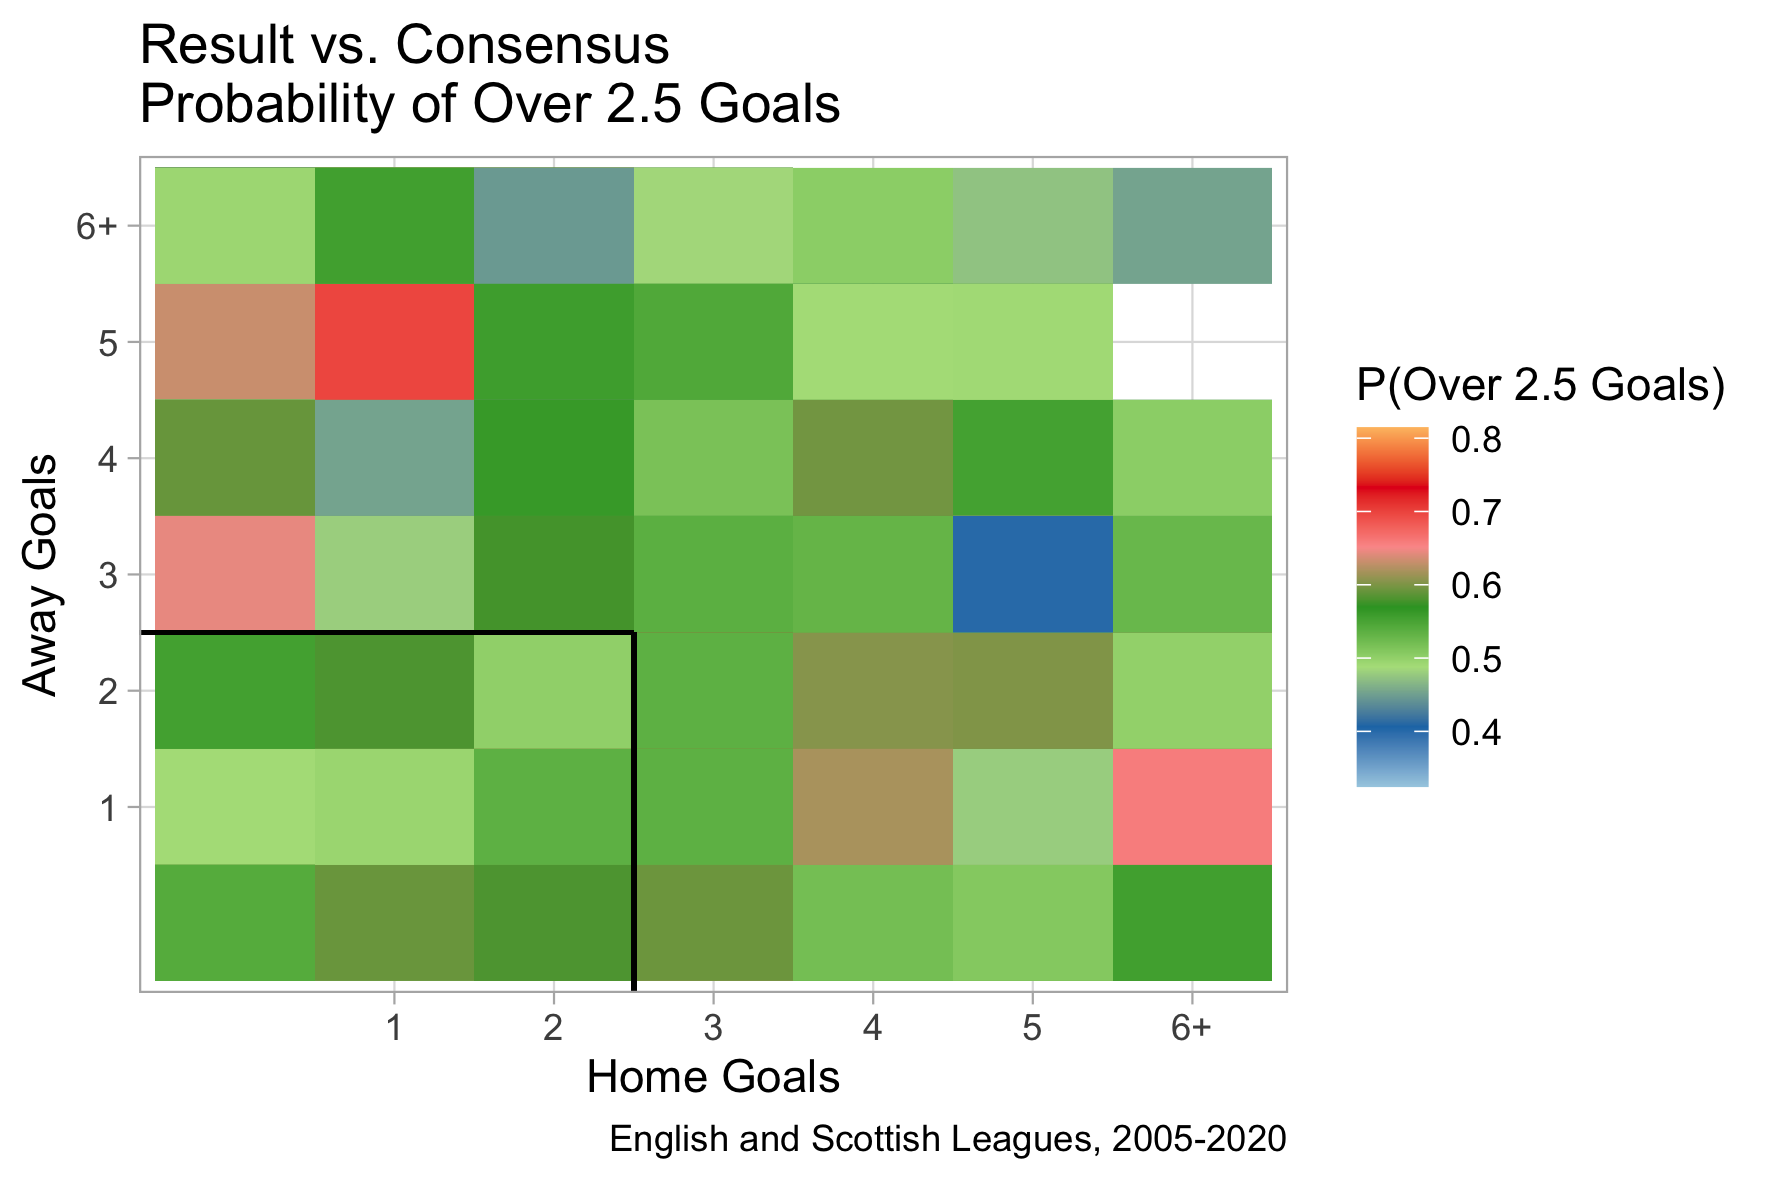
\includegraphics[width=0.7\textwidth]{ensco_07_tile_uo.png}
		\caption{Tile plot of the correct UO probability vs. the full-time result.}\label{FIG:02_03b_tile_uo}
\end{center}\end{figure}


\pagebreak
The final two exploratory plots created are \textit{count plots}. These are a way of visualising two \textsc{discrete} variables, with larger points indicating more data with the corresponding values \autocite{countPlots}. The first, Figure~\ref{FIG:02_04a_count1}, is a plot of the consensus home handicap offered for a match against the consensus probability of Over 2.5 Goals.\footnote{Rounded to 2 decimal places and considered discrete.} It would be expected that matches with a larger handicap in magnitude (bookmakers estimate these will be the most convincing matches) will have a larger consensus probability of Over 2.5 Goals. The latter, Figure~\ref{FIG:02_04b_count2}, is a plot of the expected vs. actual goal difference, where the expected is the handicap, the actual is \lstinline|FTAG| -- \lstinline|FTHG|. If the bookmakers are setting accurate handicaps, this would be expected to a linear relationship.

In both plots, the expected general trend is observed, and it can assumed, based on these two plots and Figures~\ref{FIG:02_02a_handicap_hprob} and \ref{FIG:02_02b_handicap_1x2}, that the handicaps set by bookmakers are well set. The accuracy of the markets requires further investigation.

\begin{figure}[h!]\begin{center}
		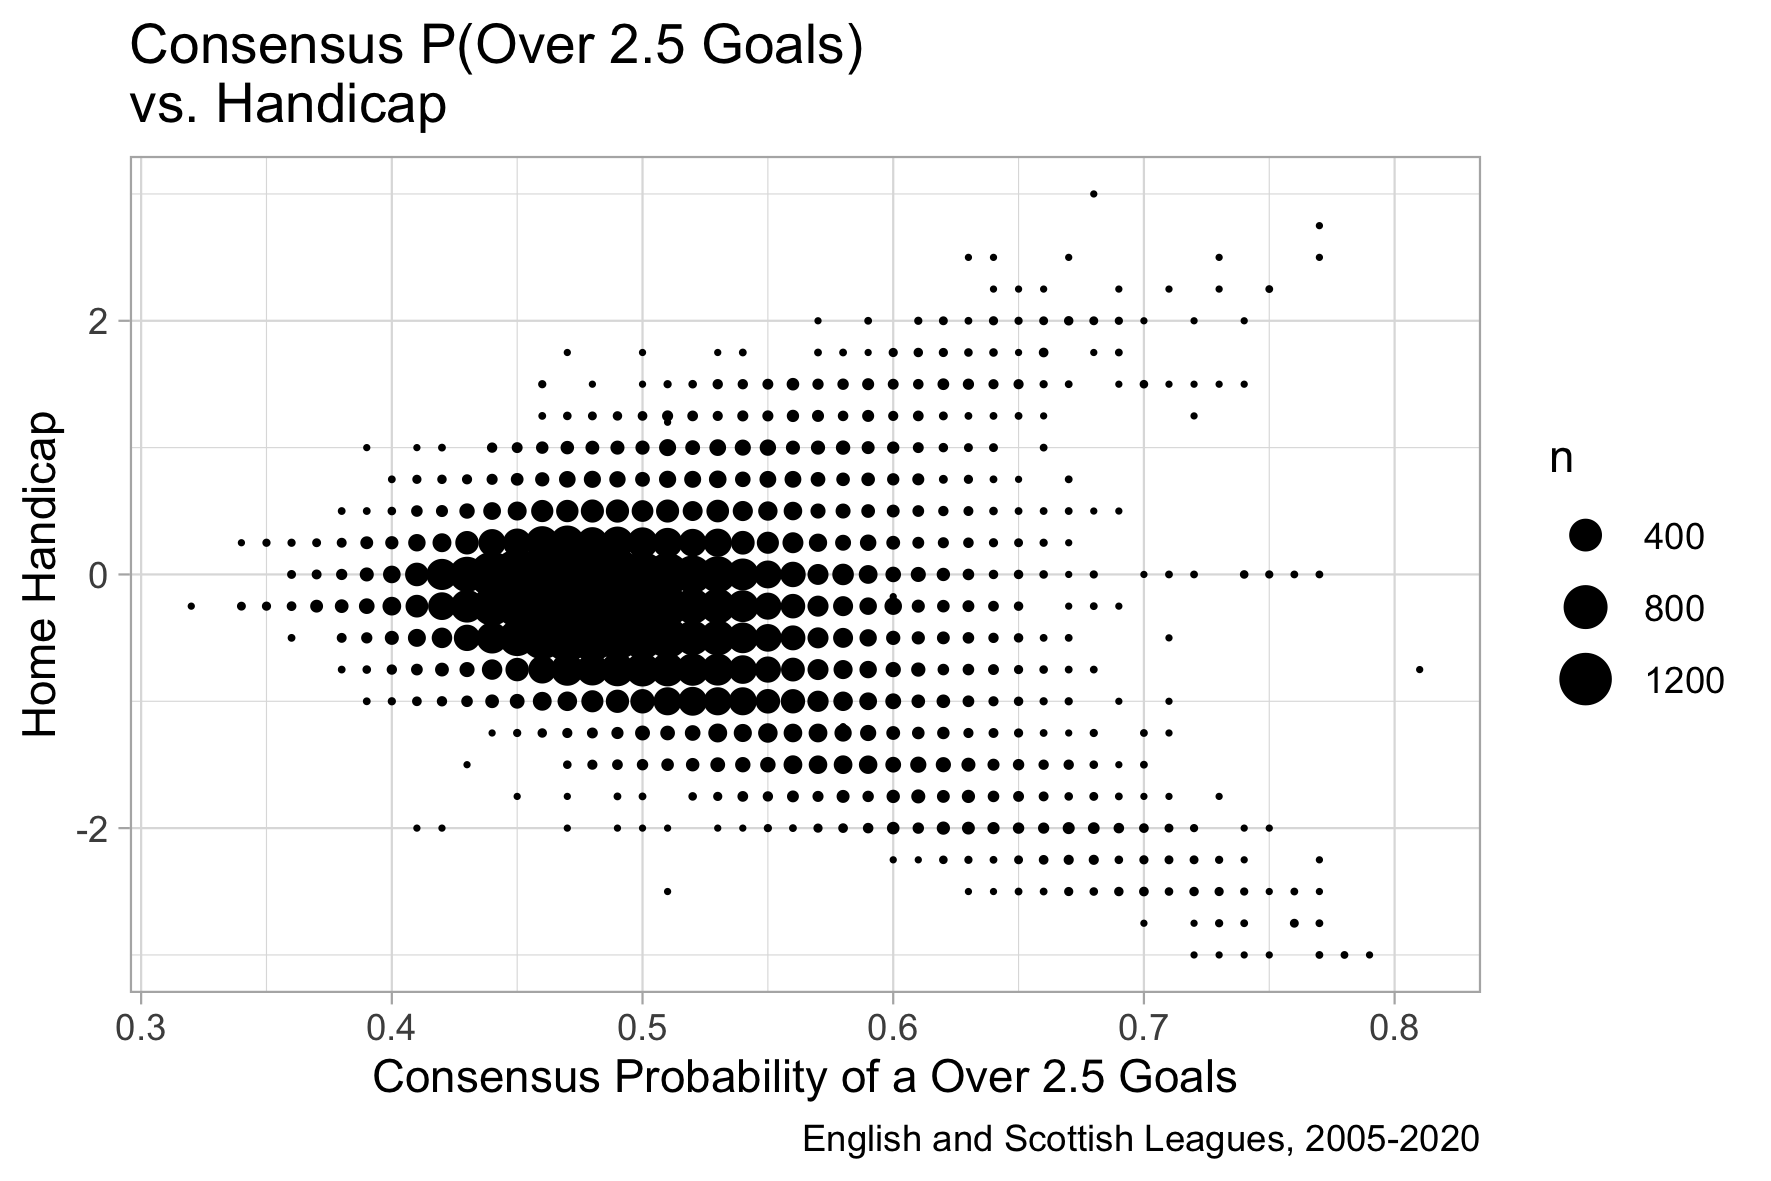
\includegraphics[width=0.6\textwidth]{ensco_08_handicap_v_over.png}
		\caption{Count plot of the home handicap offered vs. the consensus probability of over 2.5 goals.}\label{FIG:02_04a_count1}
\end{center}\end{figure}
\begin{figure}[h!]\begin{center}
		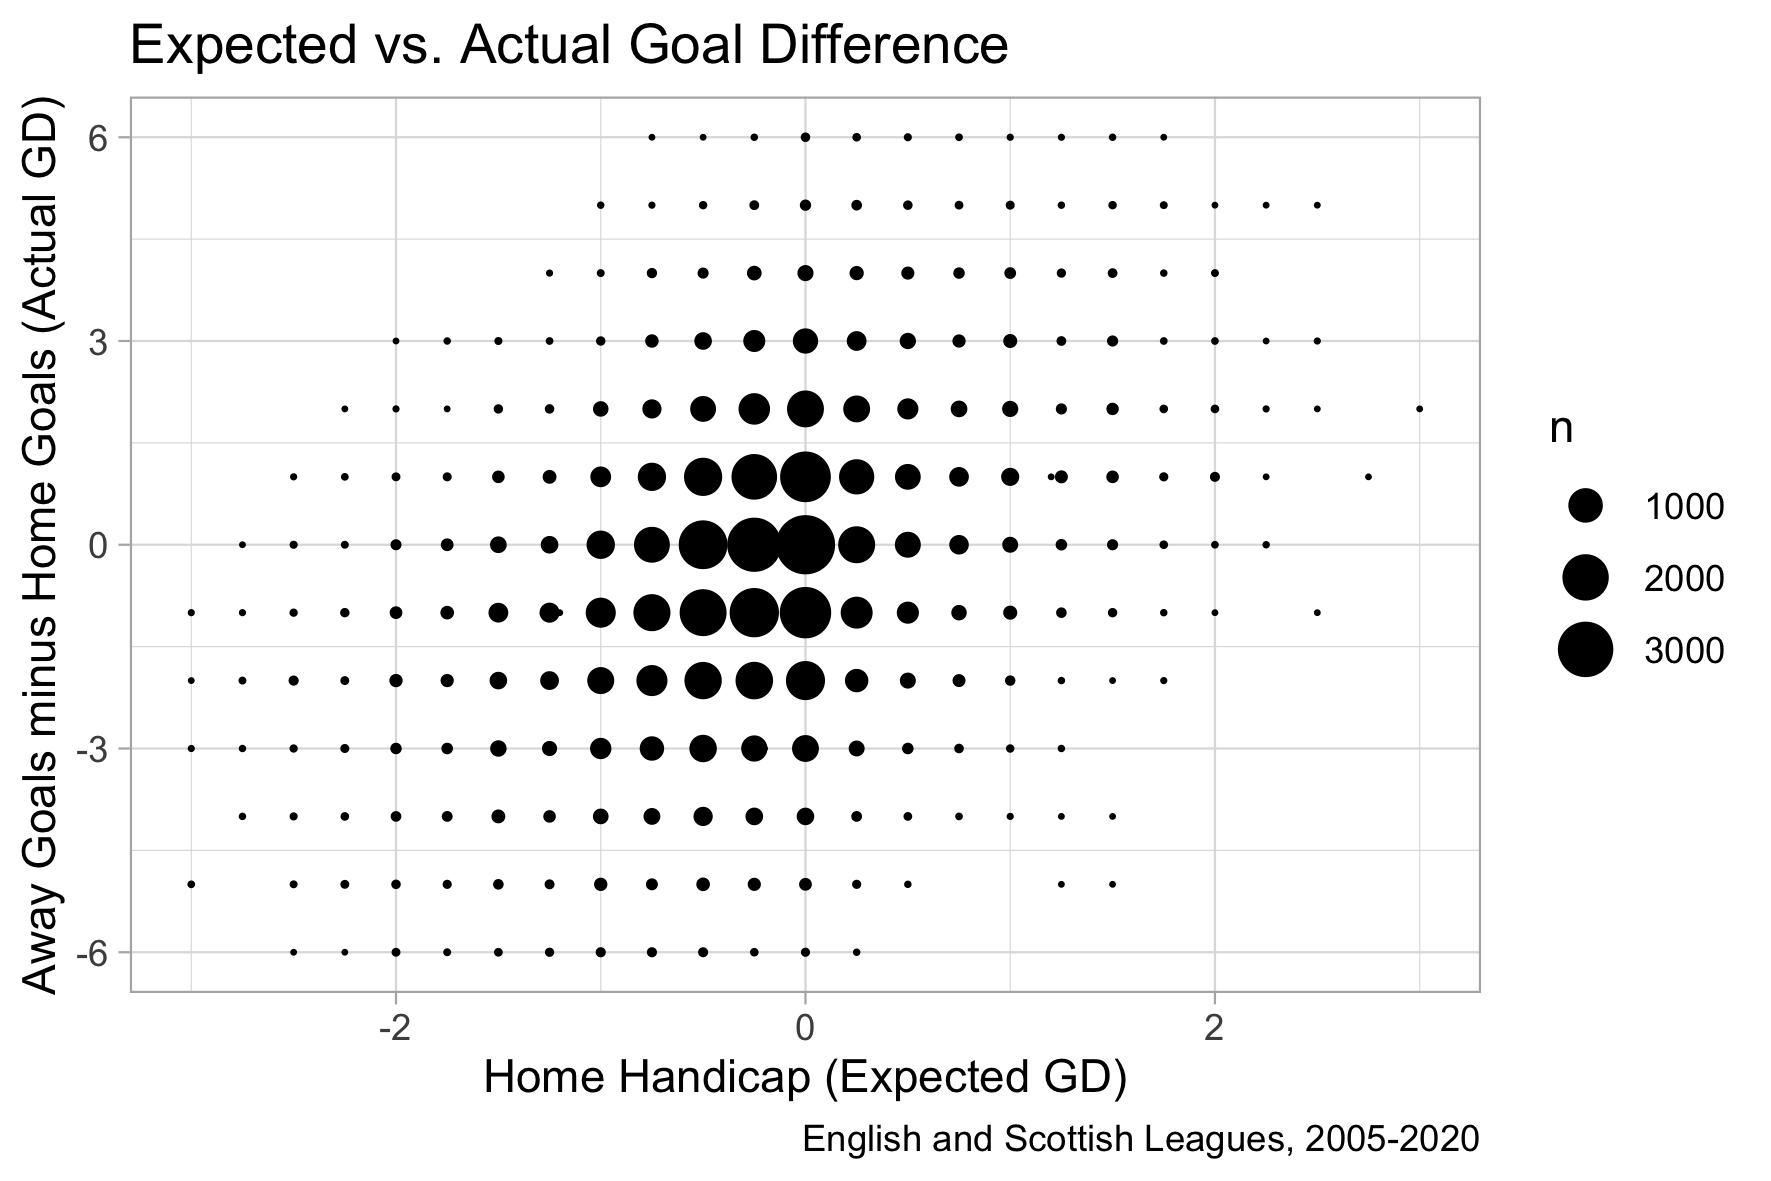
\includegraphics[width=.6\textwidth]{ensco_09_exp_v_act_goaldiff.png}
		\caption{Count plot of the expected vs. actual goal difference.}\label{FIG:02_04b_count2}
\end{center}\end{figure} 

\pagebreak

\section{Correlation Analysis} \label{sec:enscocorr}
A correlation analysis is conducted as in Chapter~\ref{ch:elite}. For all three markets, the data is first binned ($n=50$ is chosen across all markets), done in R using the \lstinline|cut| and \lstinline|tapply| commands. The observed probabilities, as defined previously as being the observed proportion of matches in a bin with the outcome of interest, of each bin are found using the \lstinline|prop.table| function. For the Asian Handicap market, only full wins are considered for ease. As the Under/Over 2.5 Goals and Asian Handicap markets are binary, only one linear model is created. The coefficients of the six final models to predict the observed probability $\mathfrak{O}$ from the consensus probability $\mathfrak{C}$ are shown in Table~\ref{tab:enscolinmods}. For `ideal' models, the gradient, or \textit{slope} of the linear model would be equal to 1.

\begin{table}[h!]\begin{center}\begin{tabular}{c||rr}
	\textit{Market} & \textit{Intercept}& \textit{Slope} \\ \hline\hline
	1X2 Home Win 	& -0.0153			& 1.0637 \\ 
	1X2 Draw		& -0.1797			& 1.9814 \\
	1X2 Away Win	& -0.0111			& 1.0462 \\
	1X2 Overall		& -0.0089			& 1.0642 \\ \hdashline
	Under/Over		&  0.0358			& 0.8463 \\
	Asian Handicap	& -0.0419			& 0.8691
\end{tabular}\end{center}\caption{Linear models to predict the observed outcome $\mathfrak{O}$ from a given bookmaker consensus probability $\mathfrak{C}$ using the English \& Scottish data.}\label{tab:enscolinmods}\end{table}

These models can be used for predictions, for example, if one was to know the consensus probabilities for an Asian Handicap bet and a Home Win 1X2 bet were both 0.6, it can be predicted that the respective observed probabilities will be 0.48 and 0.62. The models aren't much help for this use: instead, they are used to find values for the coefficient of determination $R^2$ and root-mean-square-error RMSE, and to examine the slope; these values are in Table~\ref{tab:ensco_values}. \vspace{3mm}

\begin{table}[h!]\begin{center}\begin{tabular}{c||ccc}
	&\multicolumn{3}{|c}{\textbf{1X2}} \\
	 & \textit{Home Win} & \textit{Draw} &\textit{Away Win}\\ \hline\hline
	$R^2$ 	& 0.9917 &0.5177 &0.97148 \\ 
	RMSE  	& 0.0247 &0.1602 &0.04393 \\ 
	Slope	& 1.0637 &1.9814 & 1.0462\\ \hline	
			& \textbf{Under/Over} & \textbf{Asian Handicap} & \\ \hline \hline
	$R^2$ 	& 0.3868 & 0.8959 &\\
	RMSE  	& 0.1478 & 0.0756 & \\
	Slope	& 0.8463 & 0.8691 &
\end{tabular}\end{center}\caption{Values for $R^2$, RMSE, and Slope for the markets of interest, based on the models in Table~\ref{tab:enscolinmods}.}\label{tab:ensco_values}\end{table}

The values clearly indicate poor levels of accuracy in the UO market, with $R^2 = 38.7\%$, RMSE  $=0.1478$---only lower than the RMSE for Draws in the 1X2 market---and a slope of 0.85. High levels of accuracy are found in the AH market (low RMSE, and $R^2\approx90\%$), though the slope is below the ideal, at 0.87. The 1X2 market findings are consistent with the findings outlined in Chapter~\ref{ch:elite}, with low levels of accuracy for Draws; high levels of accuracy for Home and Away Wins, both across all three measures. To visualise these findings, plots are produced. These are shown in Figures~\ref{FIG:02_convobs_1x2}, \ref{FIG:02_convobs_uo}, and \ref{FIG:02_convobs_ah}. The figures also contain the linear model and corresponding 95\% confidence interval, as defined in Appendix~\ref{app:definitionsmaths}, Definition~\ref{def:confidenceinterval}. \vspace{3mm}

The figures support the conclusions from the above values. Figure~\ref{FIG:02_convobs_1x2} has a near-perfect correlation for the Home Wins and Away Wins, corresponding to the respective $R^2$ values: 0.992 and 0.971, with the slope closely aligned to the ideal. The Draws are inaccurate, with a large confidence interval, implying a large standard error (in fact, the SE is 0.3063). In addition, the slope is visually inaccurate, corresponding to the value of 1.98. Figure~\ref{FIG:02_convobs_uo} suggests relatively high levels of accuracy in the UO market; the $R^2$ and RMSE values may be due to high values of leverage at the extremities, emphasised by the low levels of variance (Table~\ref{tab:edaenscocalcs}) in the odds offered. Figure~\ref{FIG:02_convobs_ah} also shows high levels of accuracy in the AH market, though both lines are significantly\footnote{No part of the 95\% confidence interval lies above the dotted line.} below the $y=x$ (dotted) line, possibly due to bookmaker overround. To further analyse these values, each level is considered separately.
\pagebreak 

\begin{figure}[h!]\begin{center}
	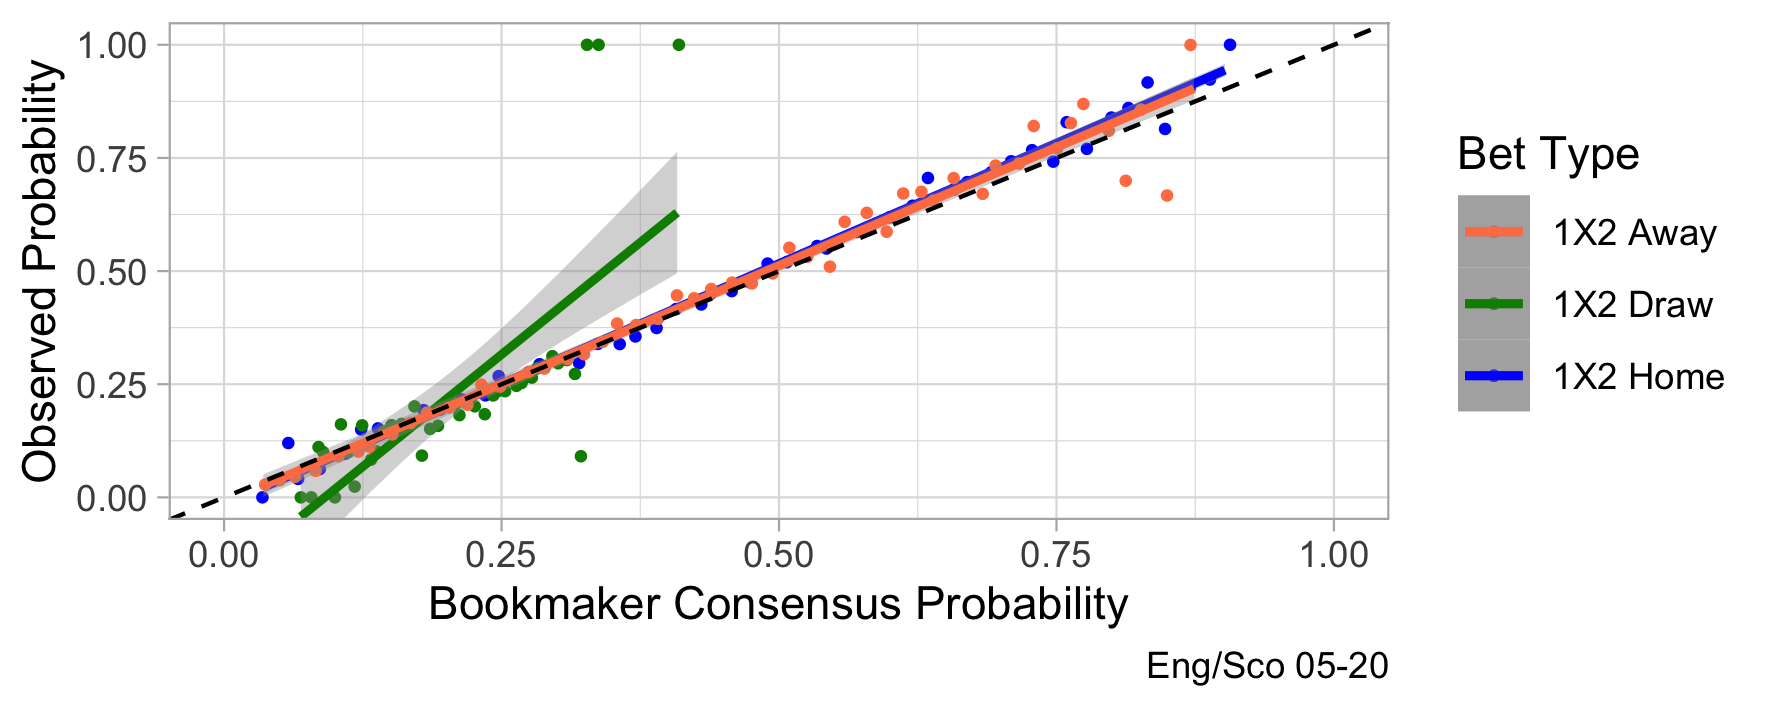
\includegraphics[width=0.75\textwidth]{ensco_10_convobs_1x2.png}
	\caption{Consensus vs. observed probabilities on the English \& Scottish data, 1X2 market.}\label{FIG:02_convobs_1x2}
\end{center}\end{figure}
\begin{figure}[h!]\begin{center}
	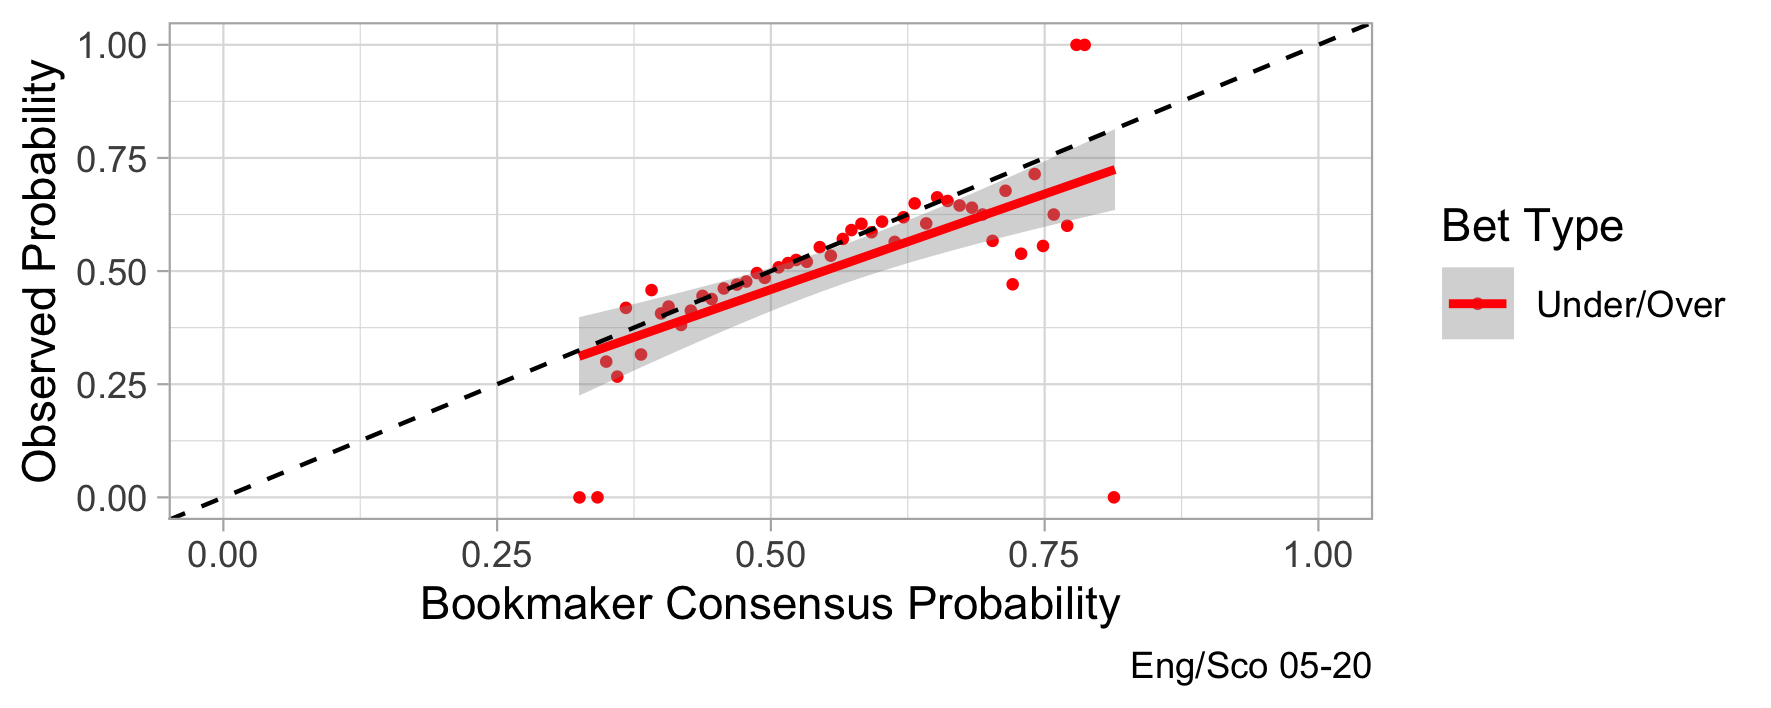
\includegraphics[width=0.75\textwidth]{ensco_11_convobs_uo.png}
	\caption{Consensus vs. observed probabilities on the English \& Scottish data, Under/Over 2.5 Goals market.}\label{FIG:02_convobs_uo}
\end{center}\end{figure}

\begin{figure}[h!]\begin{center}
	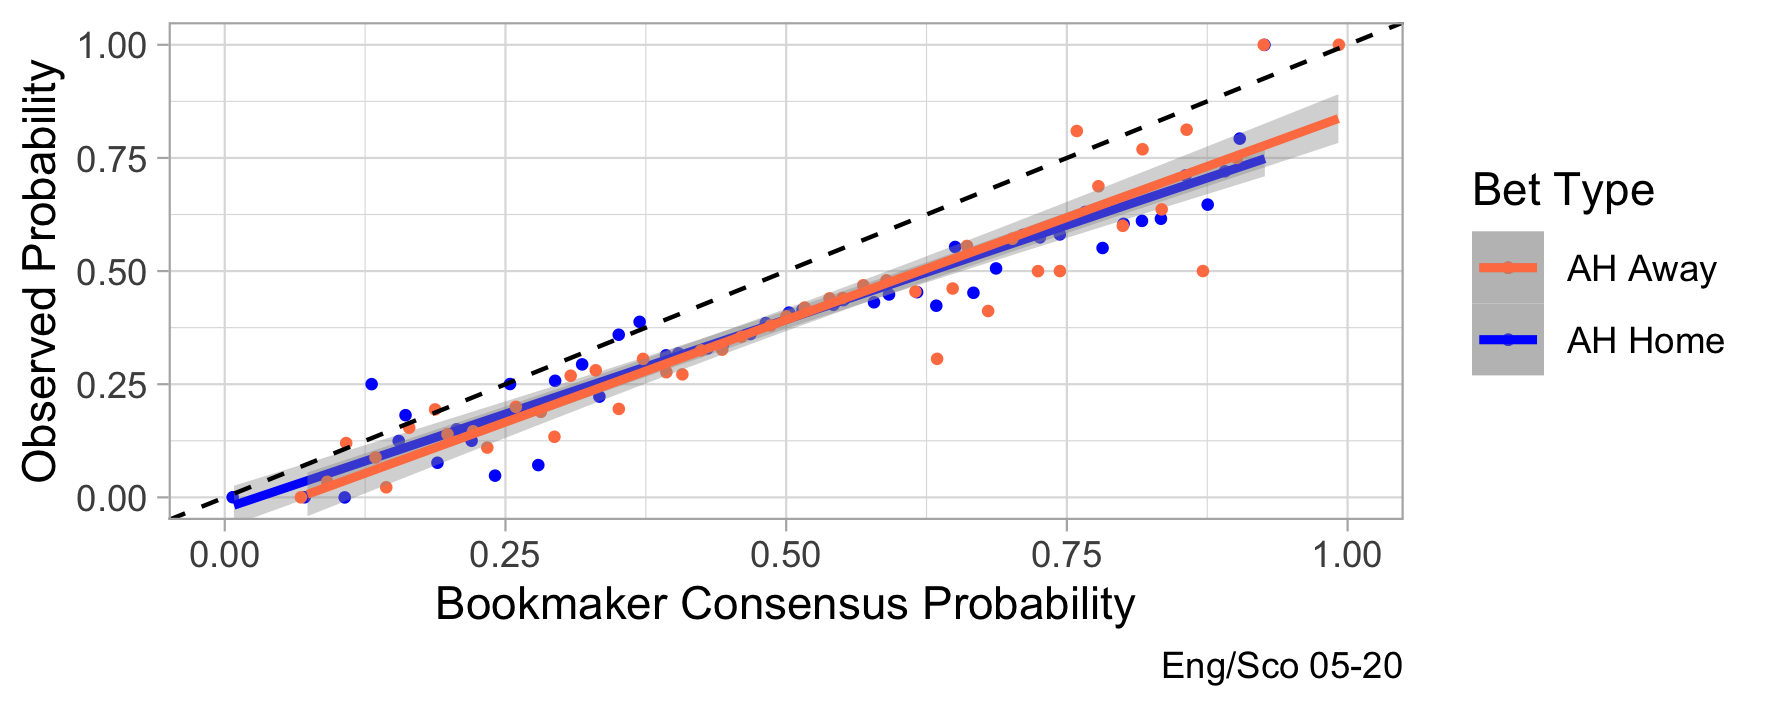
\includegraphics[width=0.75\textwidth]{ensco_12_convobs_ah.png}
	\caption{Consensus vs. observed probabilities on the English \& Scottish data, Asian Handicap market.}\label{FIG:02_convobs_ah}
\end{center}\end{figure}

\pagebreak

\section{Comparing Levels} \label{sec:enscolevels}
In addition to finding $R^2$, RMSE, and the slope, the values of $P_1$ and $P_2$ are also found for each market. As in Section~\ref{sec:elitecomparingleagues}, in order to find the values from correlation analysis, the bins are assigned a weight, with more weight given to the Home Win and Away Win bets (the matches are split into 35 bins) than to the less-varied Draw bets (15 bins). For UO and AH markets, the number of bins is 35. Plots for each are shown in Figures~\ref{FIG:02_bylevel_1}, \ref{FIG:02_bylevel_2}, and \ref{FIG:02_bylevel_3}. The values of statistical accuracy are provided in Table~\ref{tab:ensco_valuesbylevel}. 

\begin{table}[h!]\begin{center}\begin{tabular}{r||ccc}
		& \textit{Level 1} 	& \textit{Level 2} 	&\textit{Level 3} \\ \hline \hline
Number of matches $n$ 	& 17317	& 18913	& 13248 \\ \hline
\multicolumn{4}{l}{\textbf{1X2 Market}} \\ \hline
$R^2$ 					& 0.99035	& 0.75579	& 0.91903 \\
RMSE					& 0.02611 	& 0.12914 	& 0.07094 \\ 
$P_1$					& 0.36767 	& 0.35137 	& 0.35902 \\ 
$P_2$					& 0.59823 	& 0.62984 	& 0.61429 \\ 
Slope					& 1.08106	& 0.95331	& 1.04732 \\ \hline
\multicolumn{4}{l}{\textbf{Under/Over 2.5 Goals Market}} \\ \hline
$R^2$					& 0.63719	& 0.53157 	& 0.02919 \\
RMSE					& 0.10474	& 0.12414 	& 0.12980 \\ 
$P_1$					& 0.50331 	& 0.50129 	& 0.50271 \\
$P_2$					& 0.49343 	& 0.49743 	& 0.49458 \\
Slope					& 1.03996	& 1.14681	& 0.18112 \\ \hline
\multicolumn{4}{l}{\textbf{Asian Handicap Market}} \\ \hline
$R^2$					& 0.81714	& 0.76950	& 0.46815 \\
RMSE					& 0.09766	& 0.10212 	& 0.19181 \\
$P_1$					& 0.50582 	& 0.50374 	& 0.50238 \\
$P_2$		 			& 0.48920 	& 0.49277 	& 0.49534 \\
Slope					& 0.82633	& 0.86569	& 0.76894

\end{tabular}\end{center}\caption{$R^2$, RMSE, $P_1$, $P_2$, and Slope values for the 1X2, UO, and AH markets across all three levels.}\label{tab:ensco_valuesbylevel}
\end{table}

Both the figures and values suggest, in addition to having less variation, bookmaker performance is worse in Level 2 than in Level 3 in the 1X2 market, suggested by four metrics. (The slope is roughly 4.7\% away from the ideal in both, though Level 2 lies below the ideal and Level 3 is above.) Visually, the confidence intervals are larger for Level 2 than Level 3, too. Whilst the number of games in Level 3 is less ($n_{L3} = 13248 < 18913 = n_{L2}$), it is unlikely to be reason, instead being down to reasons such as the favourite-longshot bias, competitive balance,\footnote{In Level 2, all teams are professional, whereas in Level 3, there are semi-professional teams---who have have been recently promoted from regional leagues---competing against fully professional teams---such as those recently relegated---meaning the `gulf' in quality between the two may be larger between the best and worse teams in Level 3 than 2.} and/or simply bookmakers struggling more to place accurate odds on matches at Level 2 than Level 3.\vspace{3mm}

In the UO market, whilst the $P_1$ values for all three levels are higher, and the $P_2$ lower, than in the 1X2 market, the two markets cannot be compared with each other this way, as there are less options to bet on. Between levels, Level 1 has the highest $P_1$ and lowest $P_2$, indicating---as with the 1X2 market---better performance at the highest level. This is shown with the $R^2$ and RMSE values, too. The $P$-values suggest better predictive performance in Level 3 than 2, with a higher $P_1$ and lower $P_2$, and a similar RMSE value. This is not, however, replicated with the coefficient of determination, with Level 2 having an $R^2$ of 53\%, much higher than the 3\% of Level 3. The $R^2$ and RMSE across all three markets indicate poor performance. The slope is accurate in Level 1, only 0.4 from the ideal; in Level 2, this grows to 0.15, and in Level 3, this is over 0.8 below the ideal line, the worst slope across all nine market-level combinations. \vspace{3mm}

The AH market has a vastly lower $R^2$ value in Level 3, 46.8\%, than Levels 1 and 2, at 82\% and 77\% respectively. In addition, the $P_1$ values descend down the levels, and $P_2$ ascend, indicating worse performance at lower levels. Compared to the UO market, in each level, the $P_1$ is lower and $P_2$ higher for the AH market, indicating a better performance. It is worth noting that the overall $R^2$ of the AH market was shown to be 90\%, higher than all three levels. This is due to the problem of $R^2$ being reliant on the number of bins used in an analysis, though the general trend is of interest here. The values show a decrease in accuracy as lower levels are considered, with Level 3 having the lowest $R^2$, highest RMSE, and the slope furthest from the ideal. The slope is, however, more accurate in Level 2 than 1.
 
\begin{figure}[h!]\begin{center}
		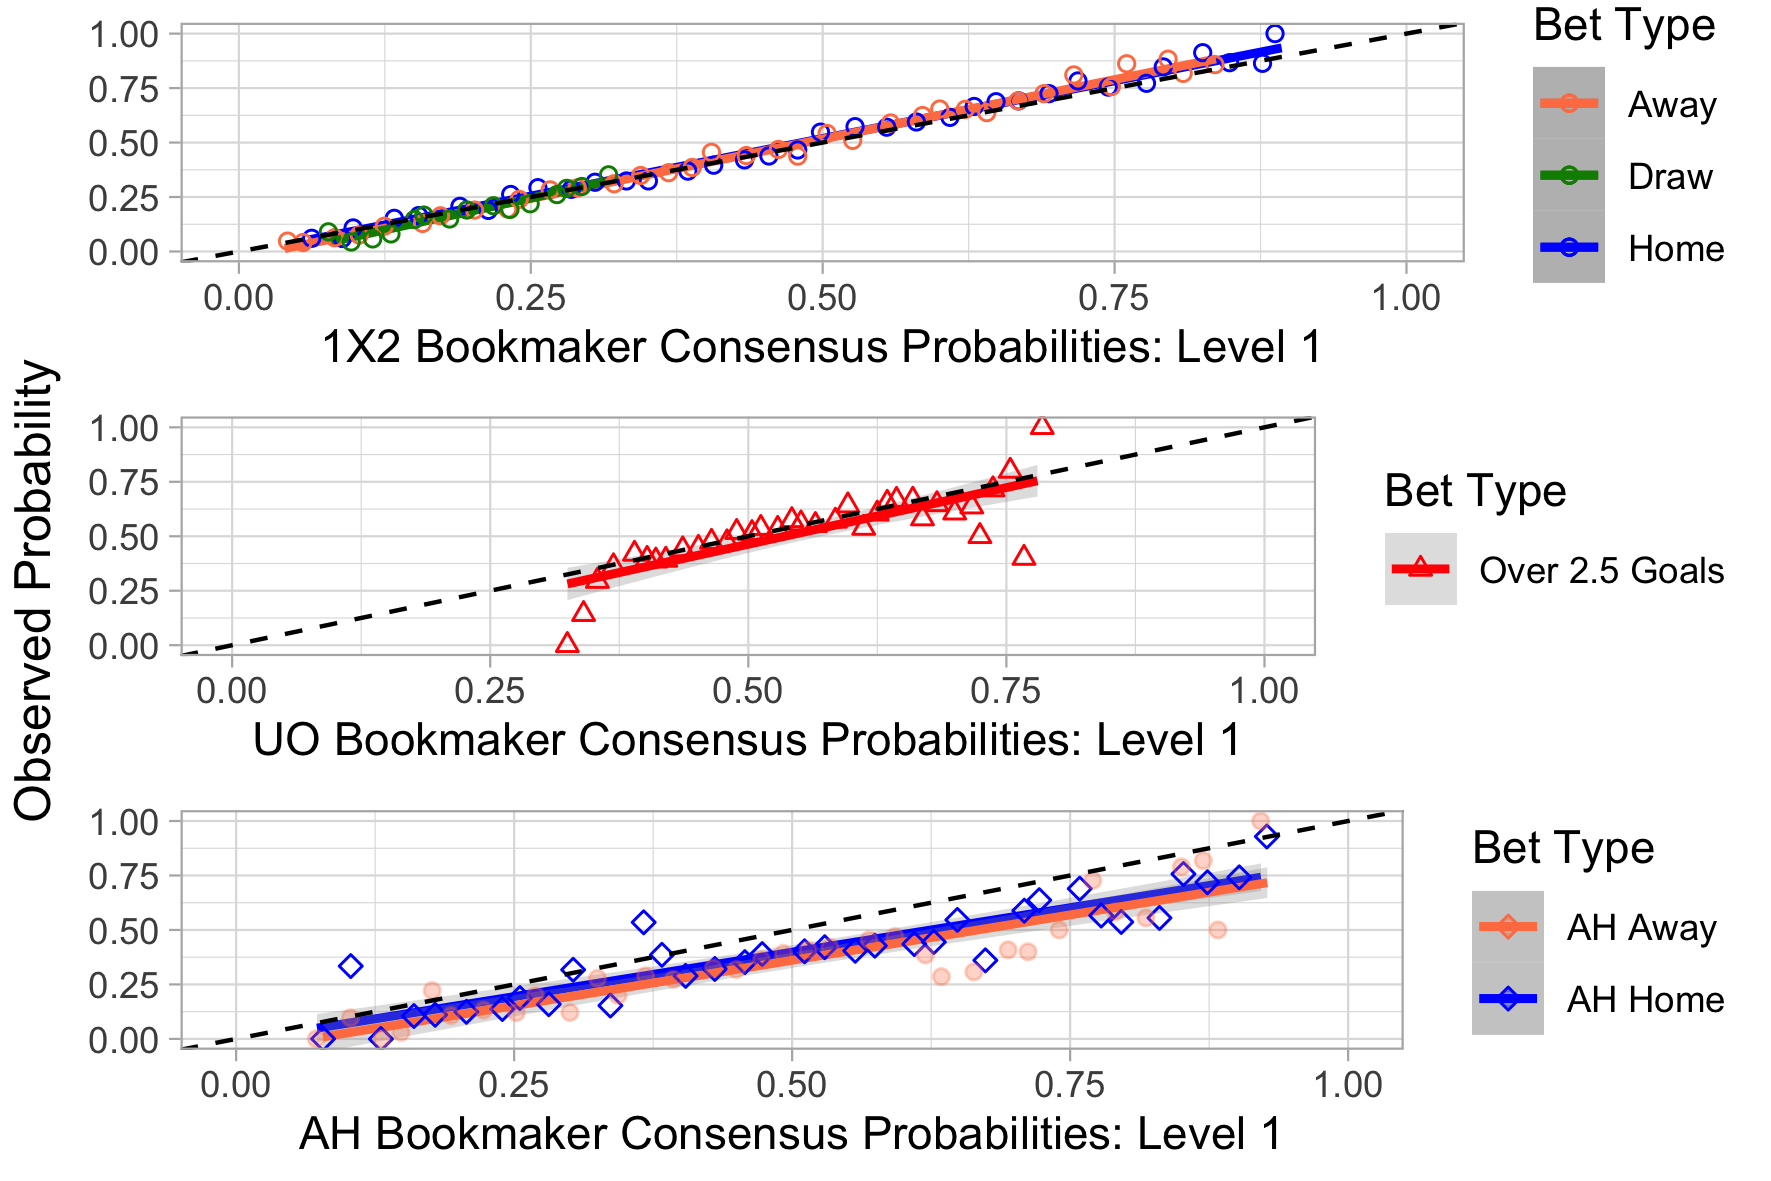
\includegraphics[width=0.82\textwidth]{ensco_13_level1.png}
		\caption{Plots of consensus vs. observed probabilities, English \& Scottish data, Level 1.}\label{FIG:02_bylevel_1}
\end{center}\end{figure}
\begin{figure}[h!]\begin{center}
		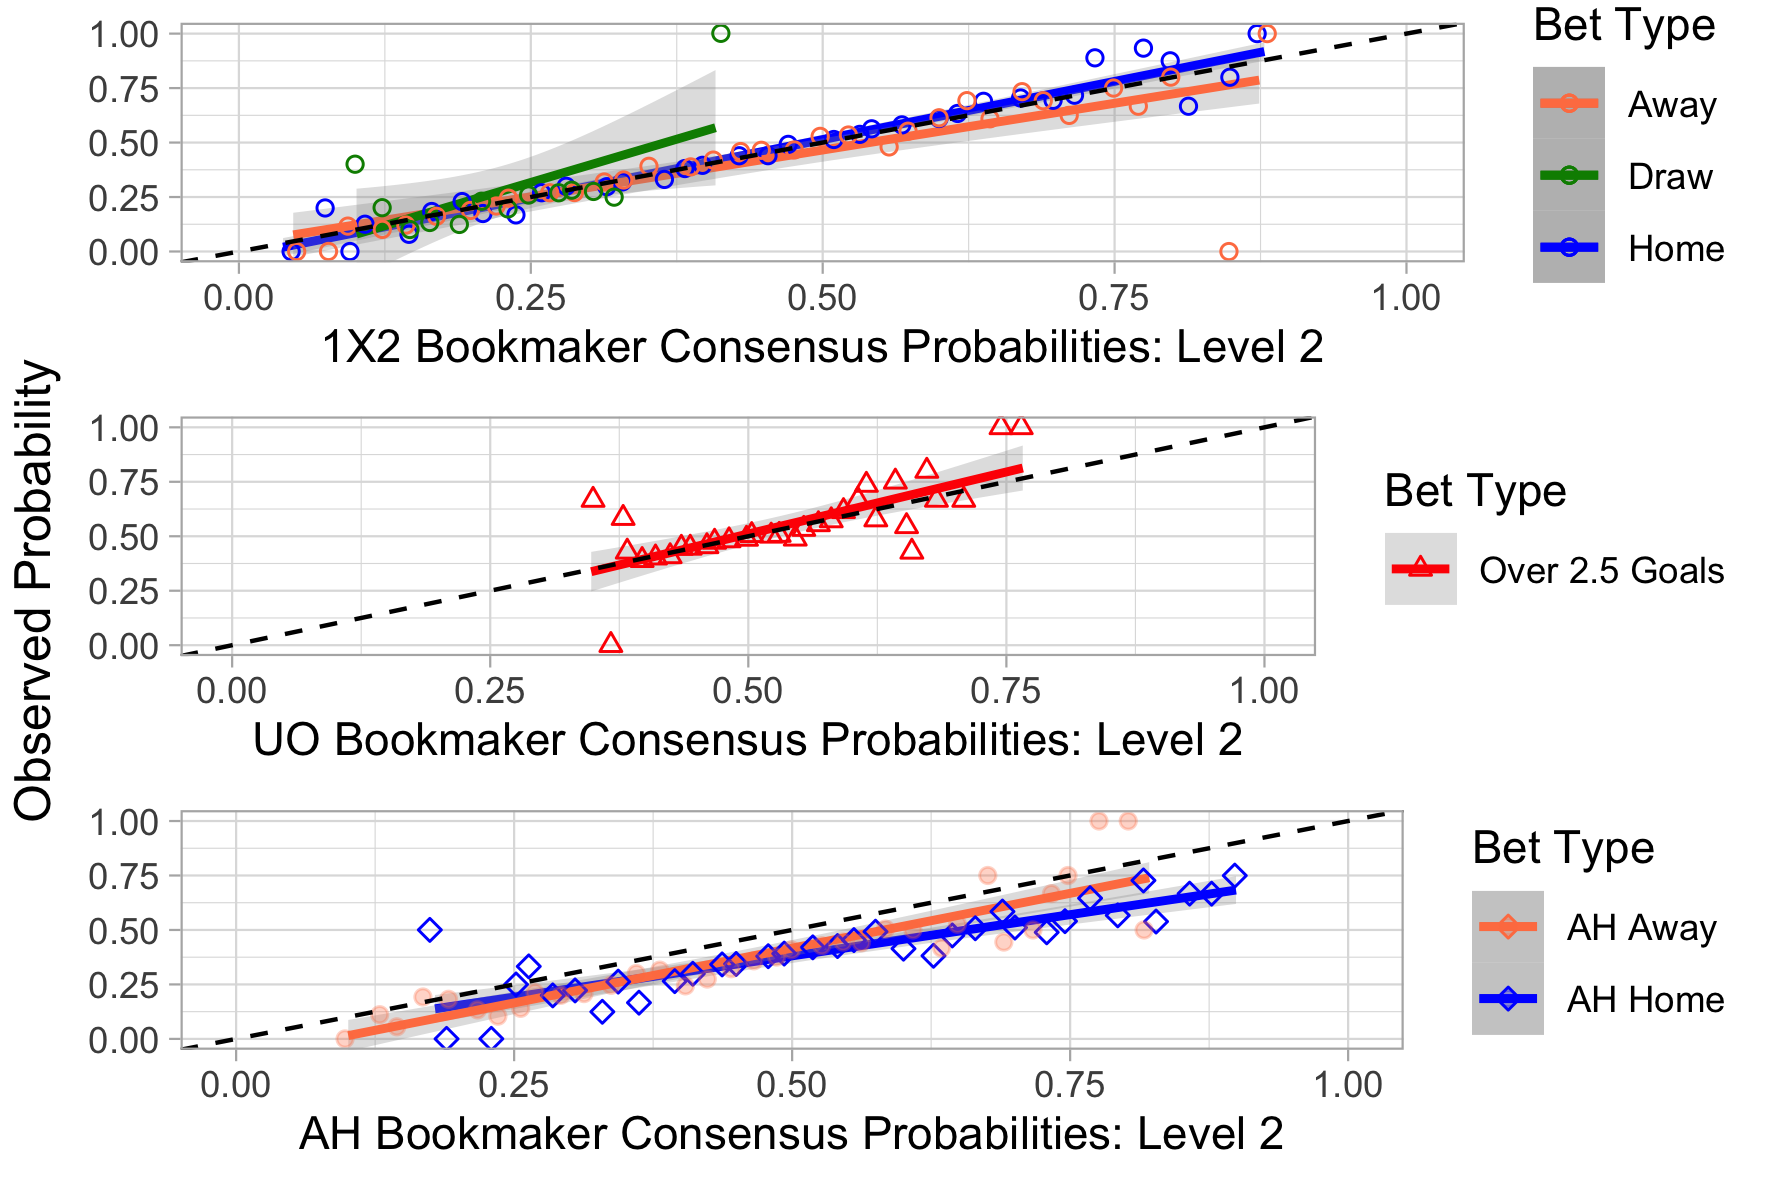
\includegraphics[width=0.82\textwidth]{ensco_13_level2.png}
		\caption{Plots of consensus vs. observed probabilities, English \& Scottish data, Level 2.}\label{FIG:02_bylevel_2}
\end{center}\end{figure}
\begin{figure}[h!]\begin{center}
		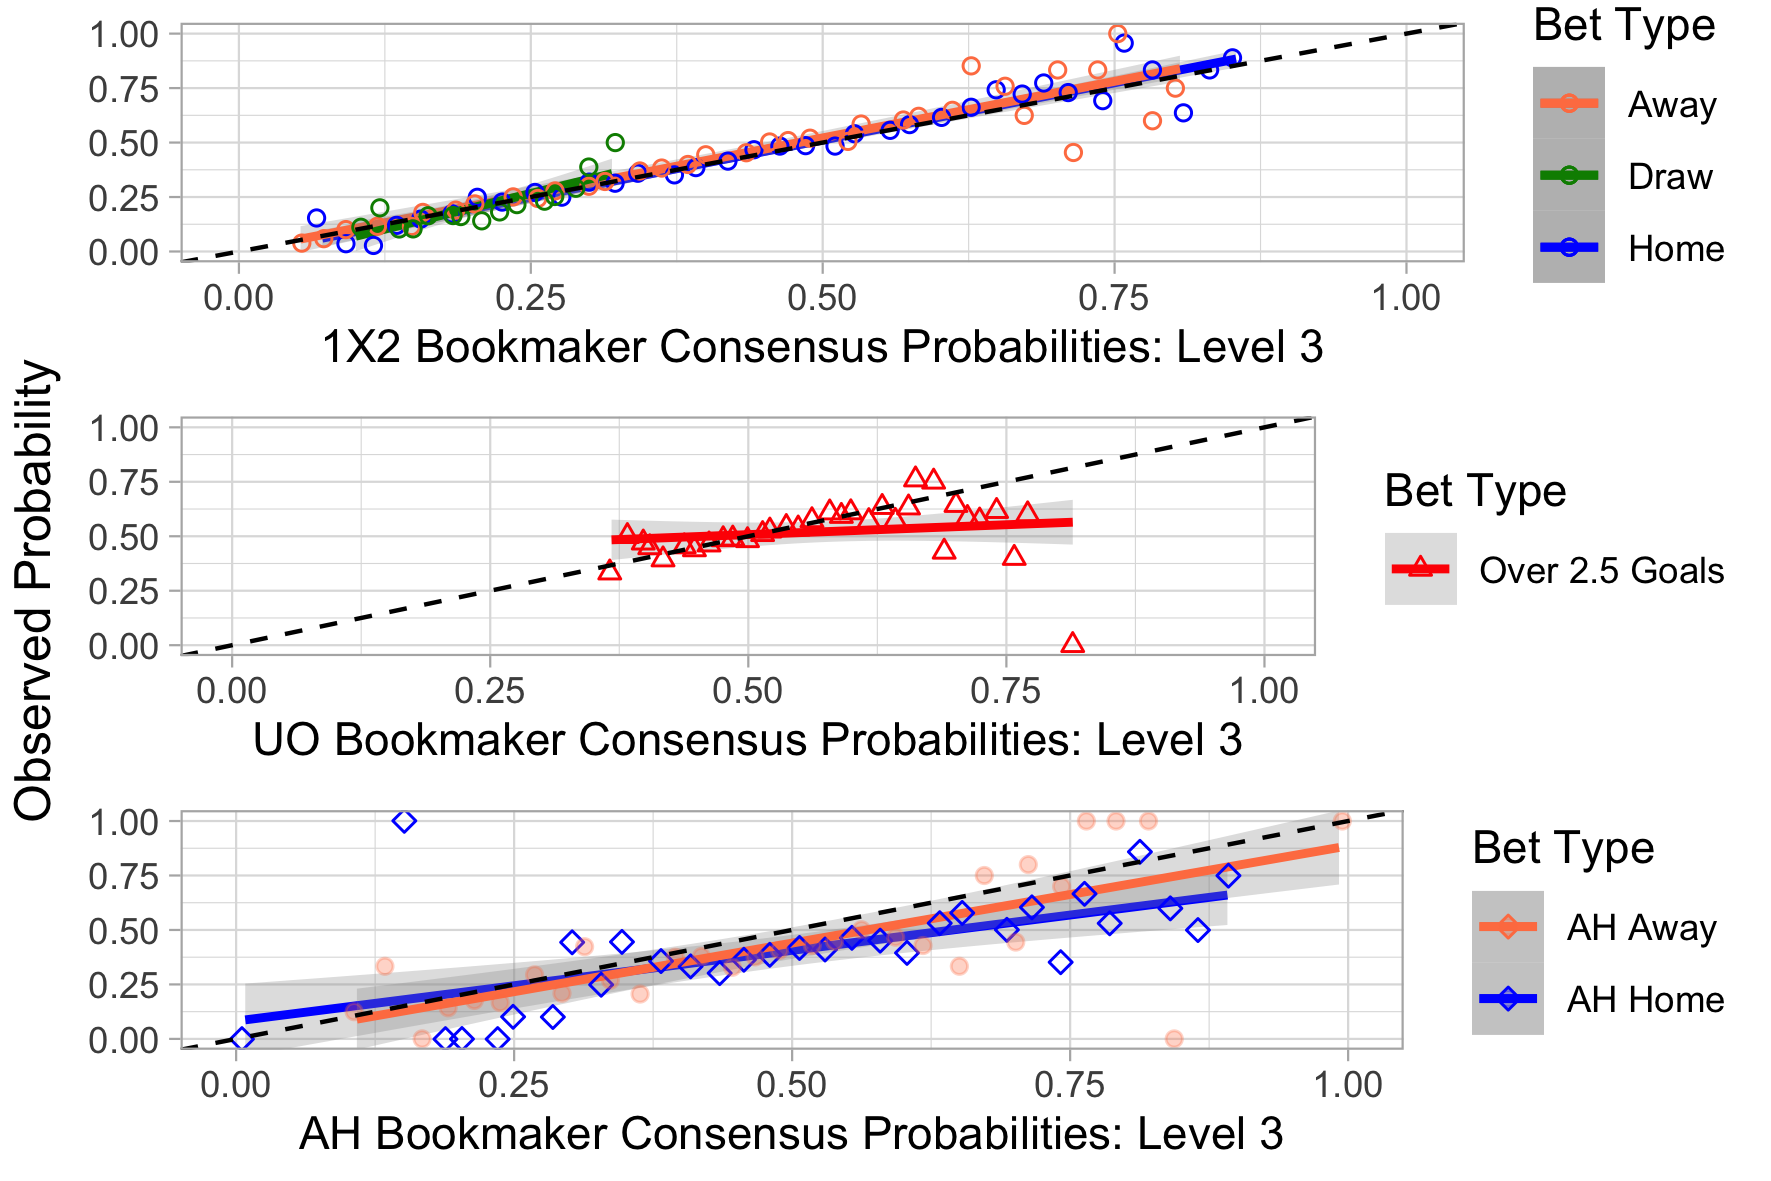
\includegraphics[width=0.82\textwidth]{ensco_13_level3.png}
		\caption{Plots of consensus vs. observed probabilities, English \& Scottish data, Level 3.}\label{FIG:02_bylevel_3}
\end{center}\end{figure}

\pagebreak
 
\section{Comparing Seasons} \label{sec:comparingseasonsensco}
As with Section~\ref{sec:comparingseasons}, the $R^2$, RMSE, $P_1$, $P_2$, and Slope values are found for each season in the 1X2 market, as well as the same five values for the UO and AH markets. These are given in Table~\ref{tab:accstatsseasons}, and displayed in Figure~\ref{FIG:02_accuracytime}, with each market's plots in a column. For the slope plots, on the fifth row, the ideal line, where the slope is equal to 1, is added in black.\vspace{3mm}

In the 1X2 market, unlike as seen previously in Section~\ref{sec:comparingseasons}, the lines of best fit for the $R^2$ and RMSE are not improving over time. It is likely, in both cases, due to two outliers: the 15/16 season ($R^2 = 87\%$, RMSE $=0.0736$) and the 17/18 season ($R^2 = 78\%$, RMSE $= 0.1200$), as opposed to an actual trend, which appears to be stable from the remaining points. The $P_1$ and $P_2$ values and the slope (which is approaching the black, ideal line at $y=1$) for the 1X2 market, however, indicate improvement over time. \vspace{3mm}

The UO market shows great improvement by the $R^2$ and RMSE metrics over time, with clear increasing and decreasing trends respectively. In addition, the $P_1$ values are increasing, and $P_2$ decreasing, against suggesting improvements. The slope is approaching the ideal, too. The UO market was found to be inaccurate in Section~\ref{sec:enscoeda}, though if this trend continues, this finding may be out-of-date soon. This could be due to improvements in modelling and new metrics/statistics such as `Expected Goals' \autocite{xgoals, xgoals2}. \vspace{3mm}

The AH, however, shows a deterioration over time across $R^2$ (decreasing) and RMSE (increasing), with the former going from a peak of 97\% in the 09/10 season to a low of 0.04\% in the 14/15 season. A potential reason for this is the decrease in variation of consensus probabilities offered in this market, which is investigated in Section~\ref{sec:overround}, Figure~\ref{FIG:02_7b_overroundah_season}. The same pattern is shown with the $P$-values, with $P_1$ decreasing and $P_2$ increasing, though both lines of best fit are skewed by the 2009/10 outlier (with the highest-ranking performance in three of the four metrics). 

\pagebreak

\begin{table}[h!]\begin{center}\begin{tabular}{c||ccccc||ccccc}
	&\multicolumn{5}{|c||}{\textbf{1X2 Market}} & \multicolumn{5}{|c}{\textbf{UO Market}} \\\hline
	\textit{Season} & $R^2$ & RMSE & $P_1$ & $P_2$ & Slope & $R^2$ & RMSE & $P_1$ & $P_2$ & Slope \\ \hline
	05/06 &0.9728 &0.0389 &0.3734 &0.5882 &1.1119 &0.0142 &0.1653 &0.5020 &0.4960 &-0.2399\\
	06/07 &0.9605 &0.0413 &0.3680 &0.5985 &1.0324 &0.0015 &0.1285 &0.5019 &0.4962 & 0.0767\\
	07/08 &0.9650 &0.0523 &0.3708 &0.5931 &1.2420 &0.7222 &0.0906 &0.5011 &0.4977 & 1.8784\\
	08/09 &0.9837 &0.0295 &0.3750 &0.5852 &1.1483 &0.0162 &0.2418 &0.5017 &0.4966 &-0.2598\\
	09/10 &0.9750 &0.0377 &0.3807 &0.5752 &1.1136 &0.0348 &0.2050 &0.5014 &0.4972 & 0.3705\\
	10/11 &0.9634 &0.0486 &0.3691 &0.5960 &1.1669 &0.0221 &0.0932 &0.5018 &0.4964 & 0.1640\\
	11/12 &0.9773 &0.0347 &0.3763 &0.5829 &1.0868 &0.8098 &0.0352 &0.5021 &0.4958 & 0.7772\\
	12/13 &0.9677 &0.0392 &0.3792 &0.5762 &0.9640 &0.4759 &0.0876 &0.5034 &0.4933 & 0.8044\\
	13/14 &0.9731 &0.0446 &0.3864 &0.5629 &1.2052 &0.7314 &0.0586 &0.5052 &0.4896 & 0.8480\\
	14/15 &0.9804 &0.0348 &0.3799 &0.5756 &1.1579 &0.1705 &0.0663 &0.5032 &0.4936 & 0.3018\\
	15/16 &0.8714 &0.0736 &0.3773 &0.5806 &0.8367 &0.8141 &0.0453 &0.5028 &0.4945 & 0.8132\\
	16/17 &0.9639 &0.0511 &0.3927 &0.5528 &1.1608 &0.0240 &0.1380 &0.5027 &0.4945 & 0.1923\\
	17/18 &0.7835 &0.1200 &0.3920 &0.5536 &1.0335 &0.8656 &0.0570 &0.5013 &0.4975 & 1.1643\\
	18/19 &0.9740 &0.0432 &0.3851 &0.5651 &1.1056 &0.7915 &0.0374 &0.5015 &0.4969 & 0.6041\\
	19/20 &0.9676 &0.0433 &0.3772 &0.5797 &0.9888 &0.9255 &0.0390 &0.5039 &0.4923 & 1.1233\\ \hline\hline
	&\multicolumn{5}{|c||}{\textbf{AH Market}} & \multicolumn{5}{|c}{ } \\\hline
	\textit{Season} & $R^2$ & RMSE & $P_1$ & $P_2$ & Slope & & & & & \\ \hline
	05/06& 0.8091& 0.1568& 0.5026& 0.4948&  1.9069&&&&&\\
	06/07& 0.7984& 0.1002& 0.5031& 0.4942&  0.9581&&&&&\\
	07/08& 0.8495& 0.0977& 0.5053& 0.4900& 0.9842&&&&&\\
	08/09& 0.8538& 0.0880& 0.5044& 0.4916&  0.7990&&&&&\\
	09/10& 0.9725& 0.0335& 0.5290& 0.4480&  0.8402&&&&&\\
	10/11& 0.6364& 0.1217& 0.5059& 0.4884&  0.7321&&&&&\\
	11/12& 0.3550& 0.1624& 0.5023& 0.4954&  1.2801&&&&&\\
	12/13& 0.0063& 0.2176& 0.5018& 0.4964&  0.0969&&&&&\\
	13/14& 0.0033& 0.2742& 0.5022& 0.4955&  0.0962&&&&&\\
	14/15& 0.0004& 0.0693& 0.5005& 0.4990& -0.0194&&&&&\\
	15/16& 0.5281& 0.1871& 0.5023& 0.4954&  1.3587&&&&&\\
	16/17& 0.1074& 0.0713& 0.5006& 0.4988&  0.3846&&&&&\\
	17/18& 0.1340& 0.1946& 0.5012& 0.4975&  0.9118&&&&&\\
	18/19& 0.2352& 0.1614& 0.5010& 0.4981&  0.9601&&&&&\\
	19/20& 0.5271& 0.1605& 0.5006& 0.4988&  1.7778
\end{tabular}
\end{center}\caption{Statistics for accuracy across each market, by season. \label{tab:accstatsseasons}}
\end{table}

\begin{figure}[hp]\begin{center}
		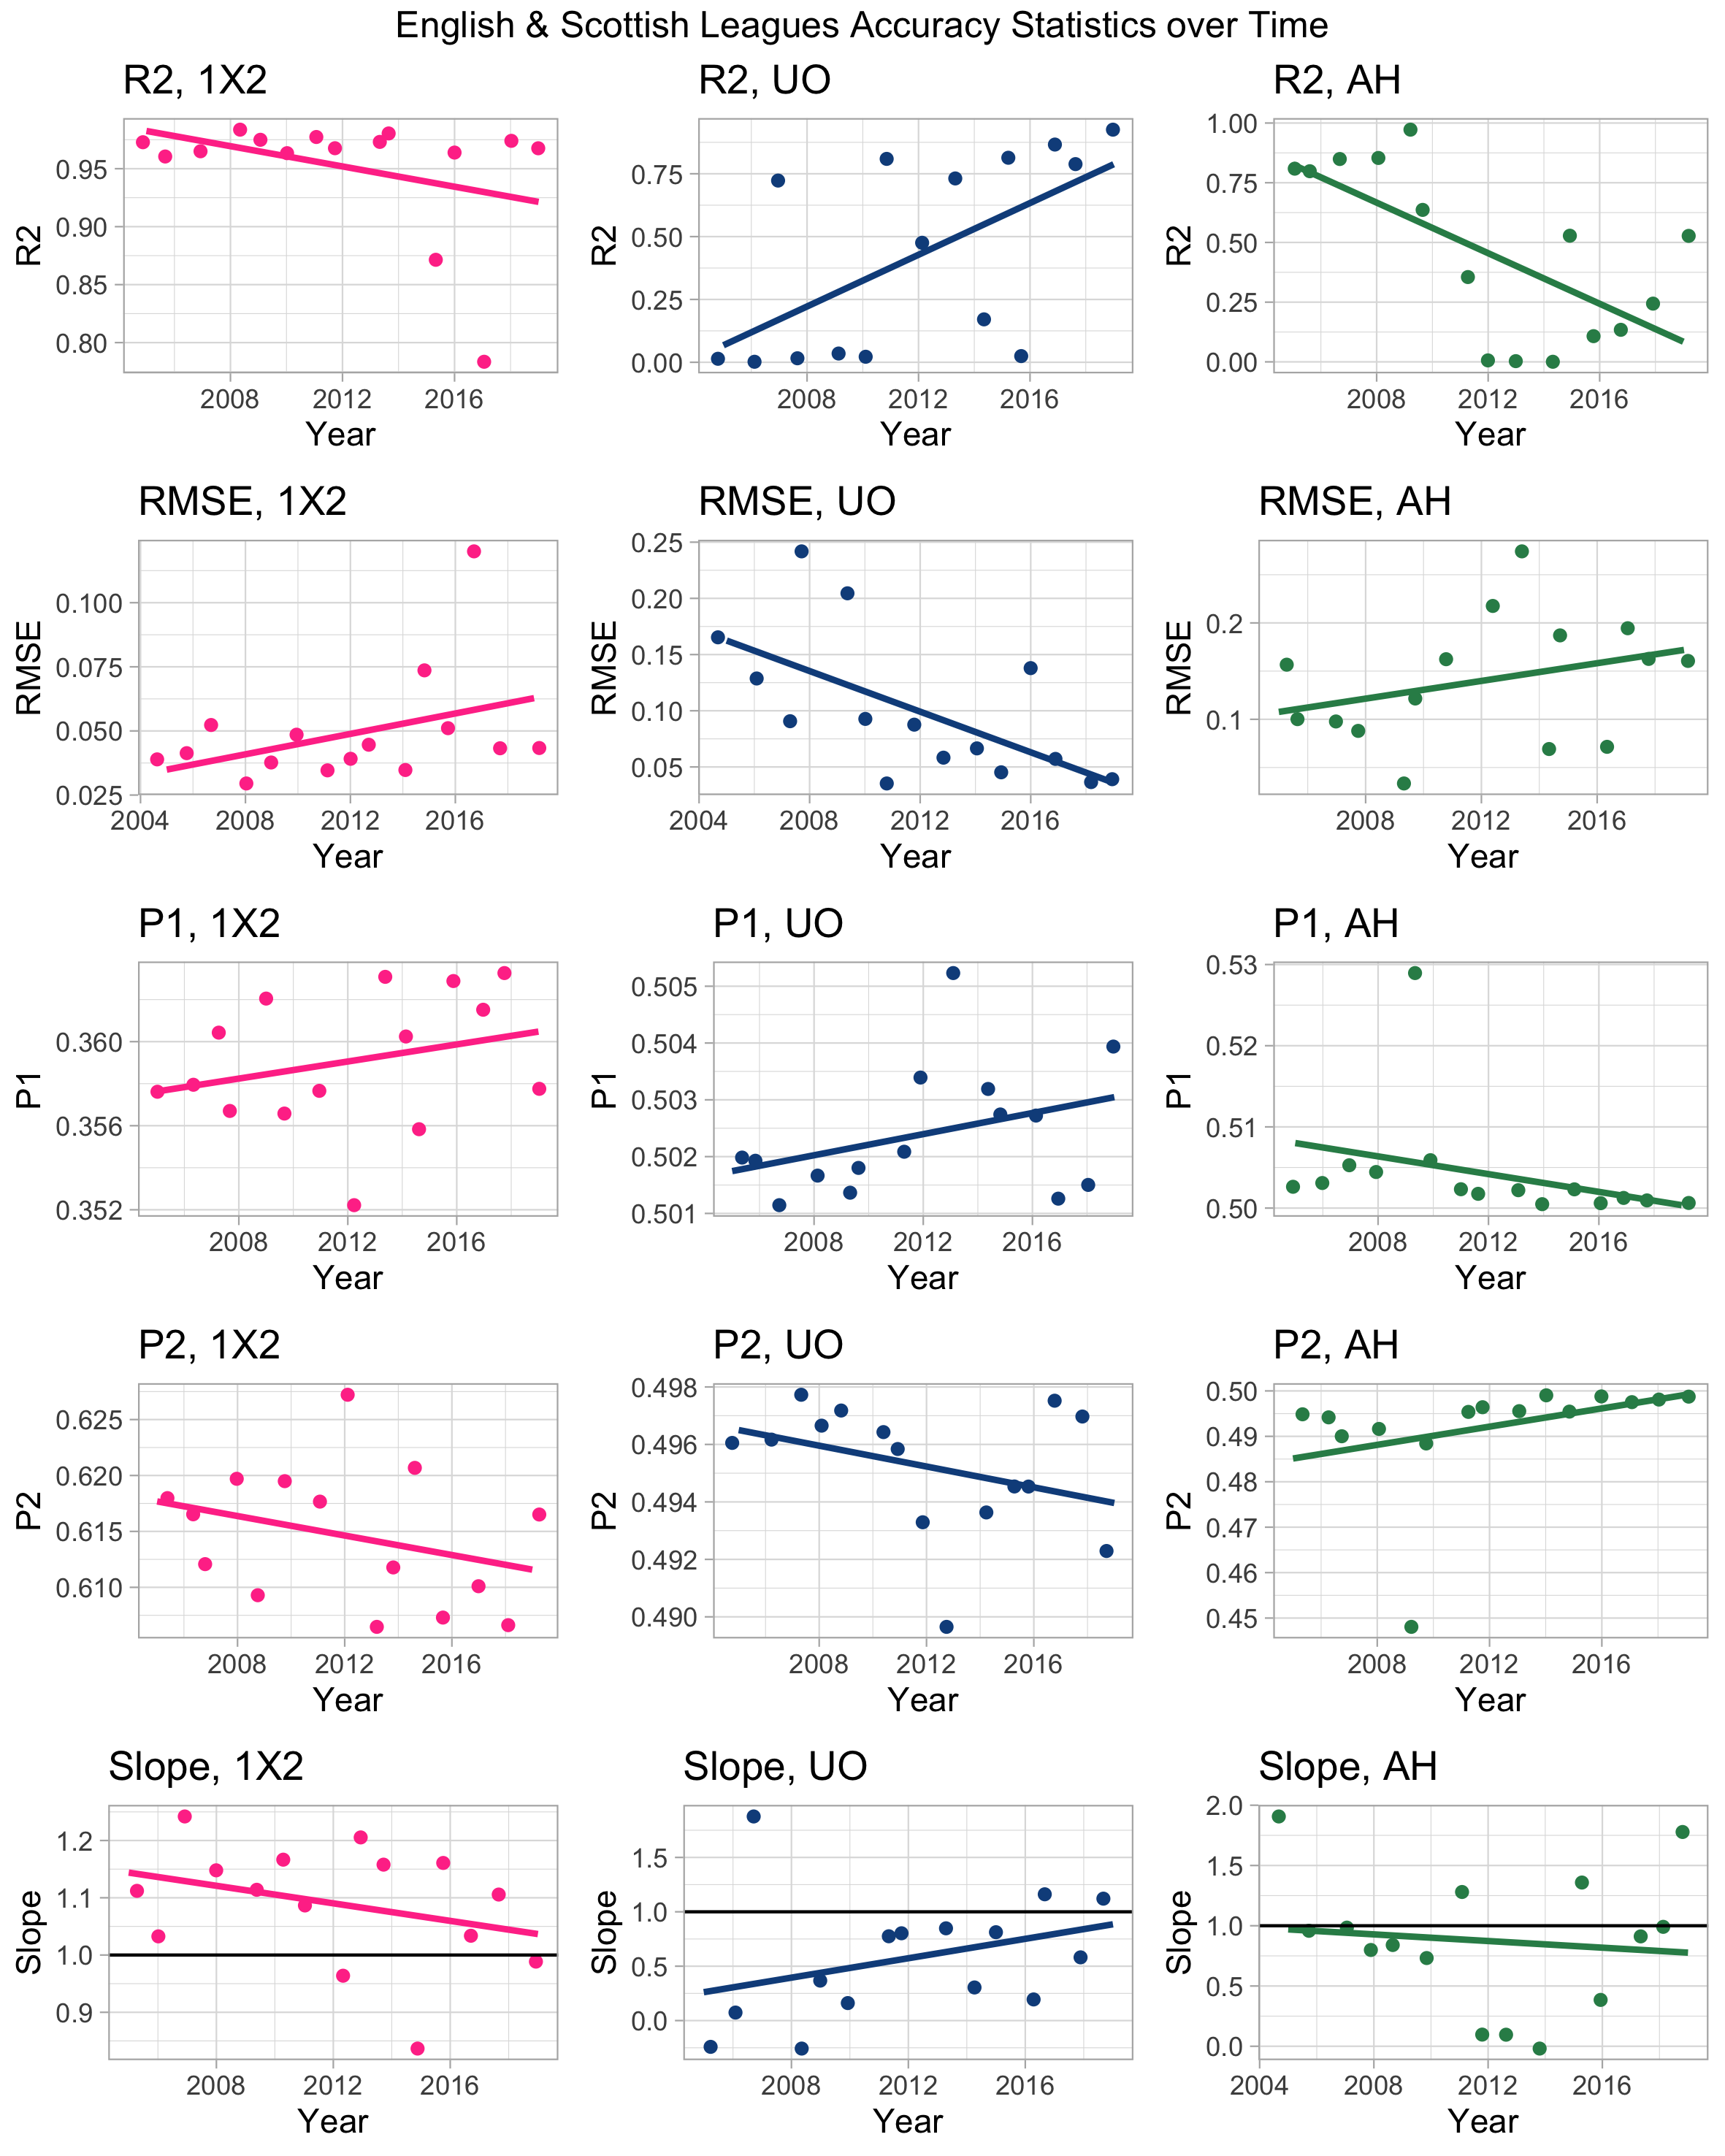
\includegraphics[width=\textwidth]{ensco_20_seasontimeplots.png}
		\caption{The variation of $R^2$, RMSE, $P_1$, $P_2$, and the Slope over time in the English \& Scottish leagues data}\label{FIG:02_accuracytime}
\end{center}\end{figure}


\pagebreak

\section{The Overround}\label{sec:overround}
The \textit{overround} $\eta$ for a single match in a market with $k$ outcomes is defined in Equation~\ref{eq:overround} \autocite{overround}. An overround of 1.05 (the sum of underlying probabilities from the odds = 1.05) represents a 5\% bookmaker commission for that match, in that market. The overround is not constant, either, and may change among `matches, bookmakers and over time' \autocite{angelini19}, as well as being disproportionate across each outcome in a single market, with bookmakers taking advantage of bettor's biases \autocite{levitt04}. As such, an assessment into the outcomes (\textsc{e.g.}, 1X2 Home Win) cannot be conducted, only the markets (\textsc{e.g.}, 1X2) as a whole. To assess where the bookmakers earn their commission, calculations and jitter/scatter plots of the overround are considered in a given market, grouped by certain variables (level and season). The values are in Table~\ref{tab:overround}; the plots are shown in Figures~\ref{FIG:02_05a_overround1x2_level} to \ref{FIG:02_7b_overroundah_season}.

\begin{equation}\label{eq:overround}
\eta = \sum^{k}_{i=1} \bigg[\frac{1}{O_i}\bigg] = \sum^{k}_{i=1}[\mathbb{P}_{\textrm{und}}(i)] 
\end{equation}

\begin{table}[h!]\begin{center}\begin{tabular}{c||cc|cc|cc}
	& \multicolumn{2}{|c|}{\textbf{1X2 Market}} & \multicolumn{2}{|c|}{\textbf{UO Market}} & \multicolumn{2}{|c}{\textbf{AH Market}}\\ \hline \hline
	Overall $\bar{\eta}$ 	& 1.0825 & 8.25\% & 1.0684 & 6.84\% & 1.0470 & 4.70\% \\ \hdashline
	Level 1 $\bar{\eta}$ 	& 1.0707 & 7.07\% & 1.0662 & 6.62\% & 1.0461 & 4.61\% \\
	Level 2 $\bar{\eta}$ 	& 1.0838 & 8.38\% & 1.0685 & 6.85\% & 1.0473 & 4.73\% \\
	Level 3 $\bar{\eta}$ 	& 1.0961 & 9.61\% & 1.0712 & 7.12\% & 1.0477 & 4.77\% \\ \hdashline
	Season 05/06 $\bar{\eta}$ & 1.1110 & 11.10\%& 1.0798 & 7.89\% & 1.0436 & 4.36\% \\
	Season 12/13 $\bar{\eta}$ & 1.0769 & 7.69\% & 1.0635 & 6.35\% & 1.0400 & 4.00\% \\
	Season 19/20 $\bar{\eta}$ & 1.0659 & 6.59\% & 1.0592 & 5.92\% & 1.0468 & 4.69\%
	\end{tabular}\end{center}\caption{The mean overround $\bar{\eta}$ for different groups of the data.}\label{tab:overround}\end{table}

\subsection*{Overround by Level}
Figures~\ref{FIG:02_05a_overround1x2_level}, \ref{FIG:02_06a_overrounduo_level}, and \ref{FIG:02_07a_overroundah_level} show the overround of each match in the 1X2, UO, and AH markets respectively, grouped by level (with red, green, and blue points for Levels 1, 2, and 3). In the 1X2 market, Level 1 has more varied overround, ranging from around 3\% to 11\%; Level 3 varies from approximately 7\% to 12\%.\footnote{It is worth noting the matches are plotted first in order of time, then in order of league, so more recent matches in Level 3 are the datapoints added last. This can be partially resolved by altering the \lstinline|alpha| (opacity) of the points. This is chosen to be 50\%.}\vspace{3mm}

In the UO market, the overround seems to be more evenly distributed, with more variation (across all levels) for matches when the odds are nearer 2 ($\mathbb{P}_{\textrm{cons}} = 0.5$), forming an almost symmetric bell curve shape. In this market, the overround is generally lower than for the 1X2 market, varying from just around 2.5\% to just over 12\%, with the majority around 5\% to 7\%. Level 1 odds vary less than Levels 2 and 3, too. \vspace{3mm}

The AH market has a less varied overround. The majority of matches exist between 5\% and 10\%; when the consensus probability is near 0.5, however, the overround appears to decrease to a low of around 1\%. This pattern holds across all three levels.\vspace{3mm}

These findings are backed up by the values in Table~\ref{tab:overround}. In the 1X2 market, the mean overround in Level 1 is 7.1\%, whereas in Level 3, this rises to 9.6\%. In the UO market, it rises from 6.6\% in Level 1 to 7.1\% in Level 3; for the AH market, it is more stable, rising from 4.6\% to 4.8\%.

\subsection*{Overround by Season}
The shape of these figures will be identical to those for overround by Level in their respective markets. Figures~\ref{FIG:02_05b_overround1x2_season}, \ref{FIG:02_06b_overrounduo_season}, and \ref{FIG:02_7b_overroundah_season} show the overround of each match, grouped by season, with the colour of the data points following the colours of a rainbow: reds and yellows are for earlier seasons, greens and blues for `middle' seasons, and violets and pinks for later (more-recent) seasons. \vspace{3mm}

In the 1X2 market \ref{FIG:02_05b_overround1x2_season}, overround is decreasing over time, with the maximum overround decreasing from around 12\% for the earliest seasons in the data to around 10\%. The floor of the range hasn't moved from around 4\%, however.\vspace{3mm}

In the UO market, the variation in the overround has decreased massively: the pink datapoints for the 19/20 season cover a range from 5\% to 7\%. At the bulge when $\mathbb{P}_{\textrm{cons}}\approx0.5$, the matches that lie above or below this range are generally from earlier seasons, varying from around 2.5\% to just over 12\%. \vspace{3mm}

From Figure~\ref{FIG:02_7b_overroundah_season}, the most striking change is in the variation in consensus probabilities: these range from around 0.12 to 0.80 for the `middle'/green datapoints, reducing to a high concentration around 0.4 to 0.6 in more recent (pink) seasons, indicating as time progresses, bookmaker handicap selection is improving. The overround is slightly decreased too in the `bulge' with this high-concentration area having an overround around 3\% to 6\% in recent seasons and 2\% to 10\% in older seasons; the green band from 0.12 to 0.80 has a higher overround, around 6\% to 10\%.\vspace{3mm}

The values in Table~\ref{tab:overround} again back this up. Over time, the mean 1X2 overround has decreased from 11.1\% to 6.6\% and the mean UO overround from 8.0\% to 5.9\%. The mean AH overround has changed from 4.4\% to 4.7\%, despite being as low as 4.0\% in 2012/13 (half-way through the dataset). \vspace{3mm}

\subsection*{Summary of Findings}
To summarise, the overround is reduced at higher levels, across all three markets: this is most evident in the 1X2 market (where the mean Level 3 overround is 2.54\% higher than Level 1), and is least evident in the Asian Handicap market (0.16\%). Over time, the overround has been reducing the 1X2 and Under/Over 2.5 Goals markets, but remaining stable in the Asian Handicap: the largest change in the AH market is the variance of the consensus probability (and thus, odds offered), which have been reducing over time.

\pagebreak

\subsection*{Overround Plots}
\begin{figure}[h!]\begin{center}
		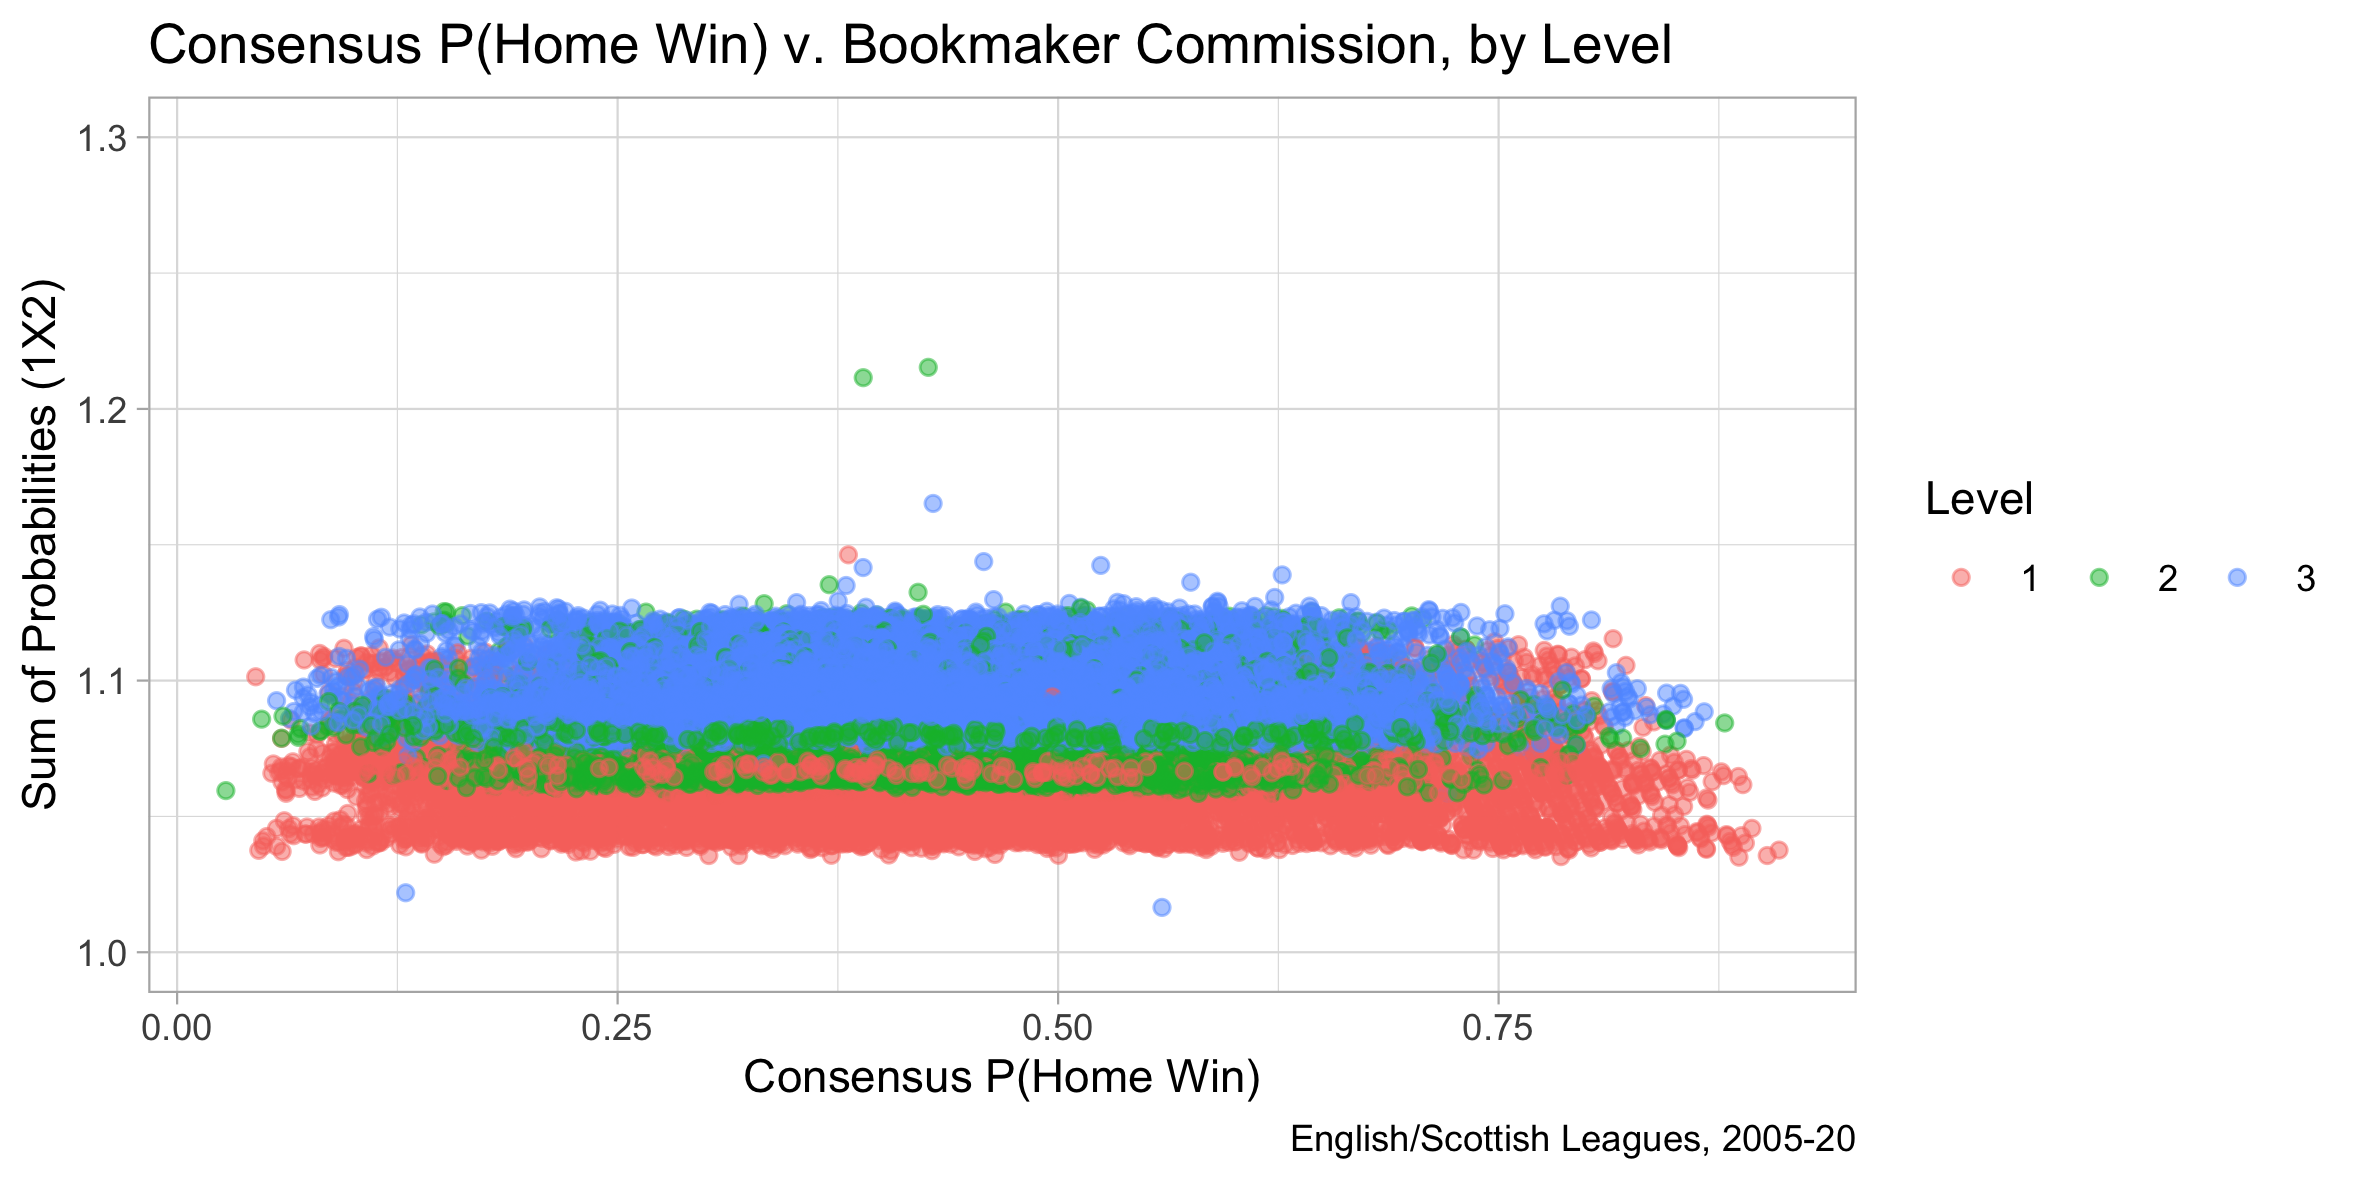
\includegraphics[width=0.9\textwidth]{ensco_14a_overround_ot_l.png}  
		\caption{The overround in the 1X2 market vs. $\mathbb{P}_{\textrm{cons}}$(1X2 Home Win), split by level.}\label{FIG:02_05a_overround1x2_level}
\end{center}\end{figure}
\begin{figure}[h!]\begin{center}
		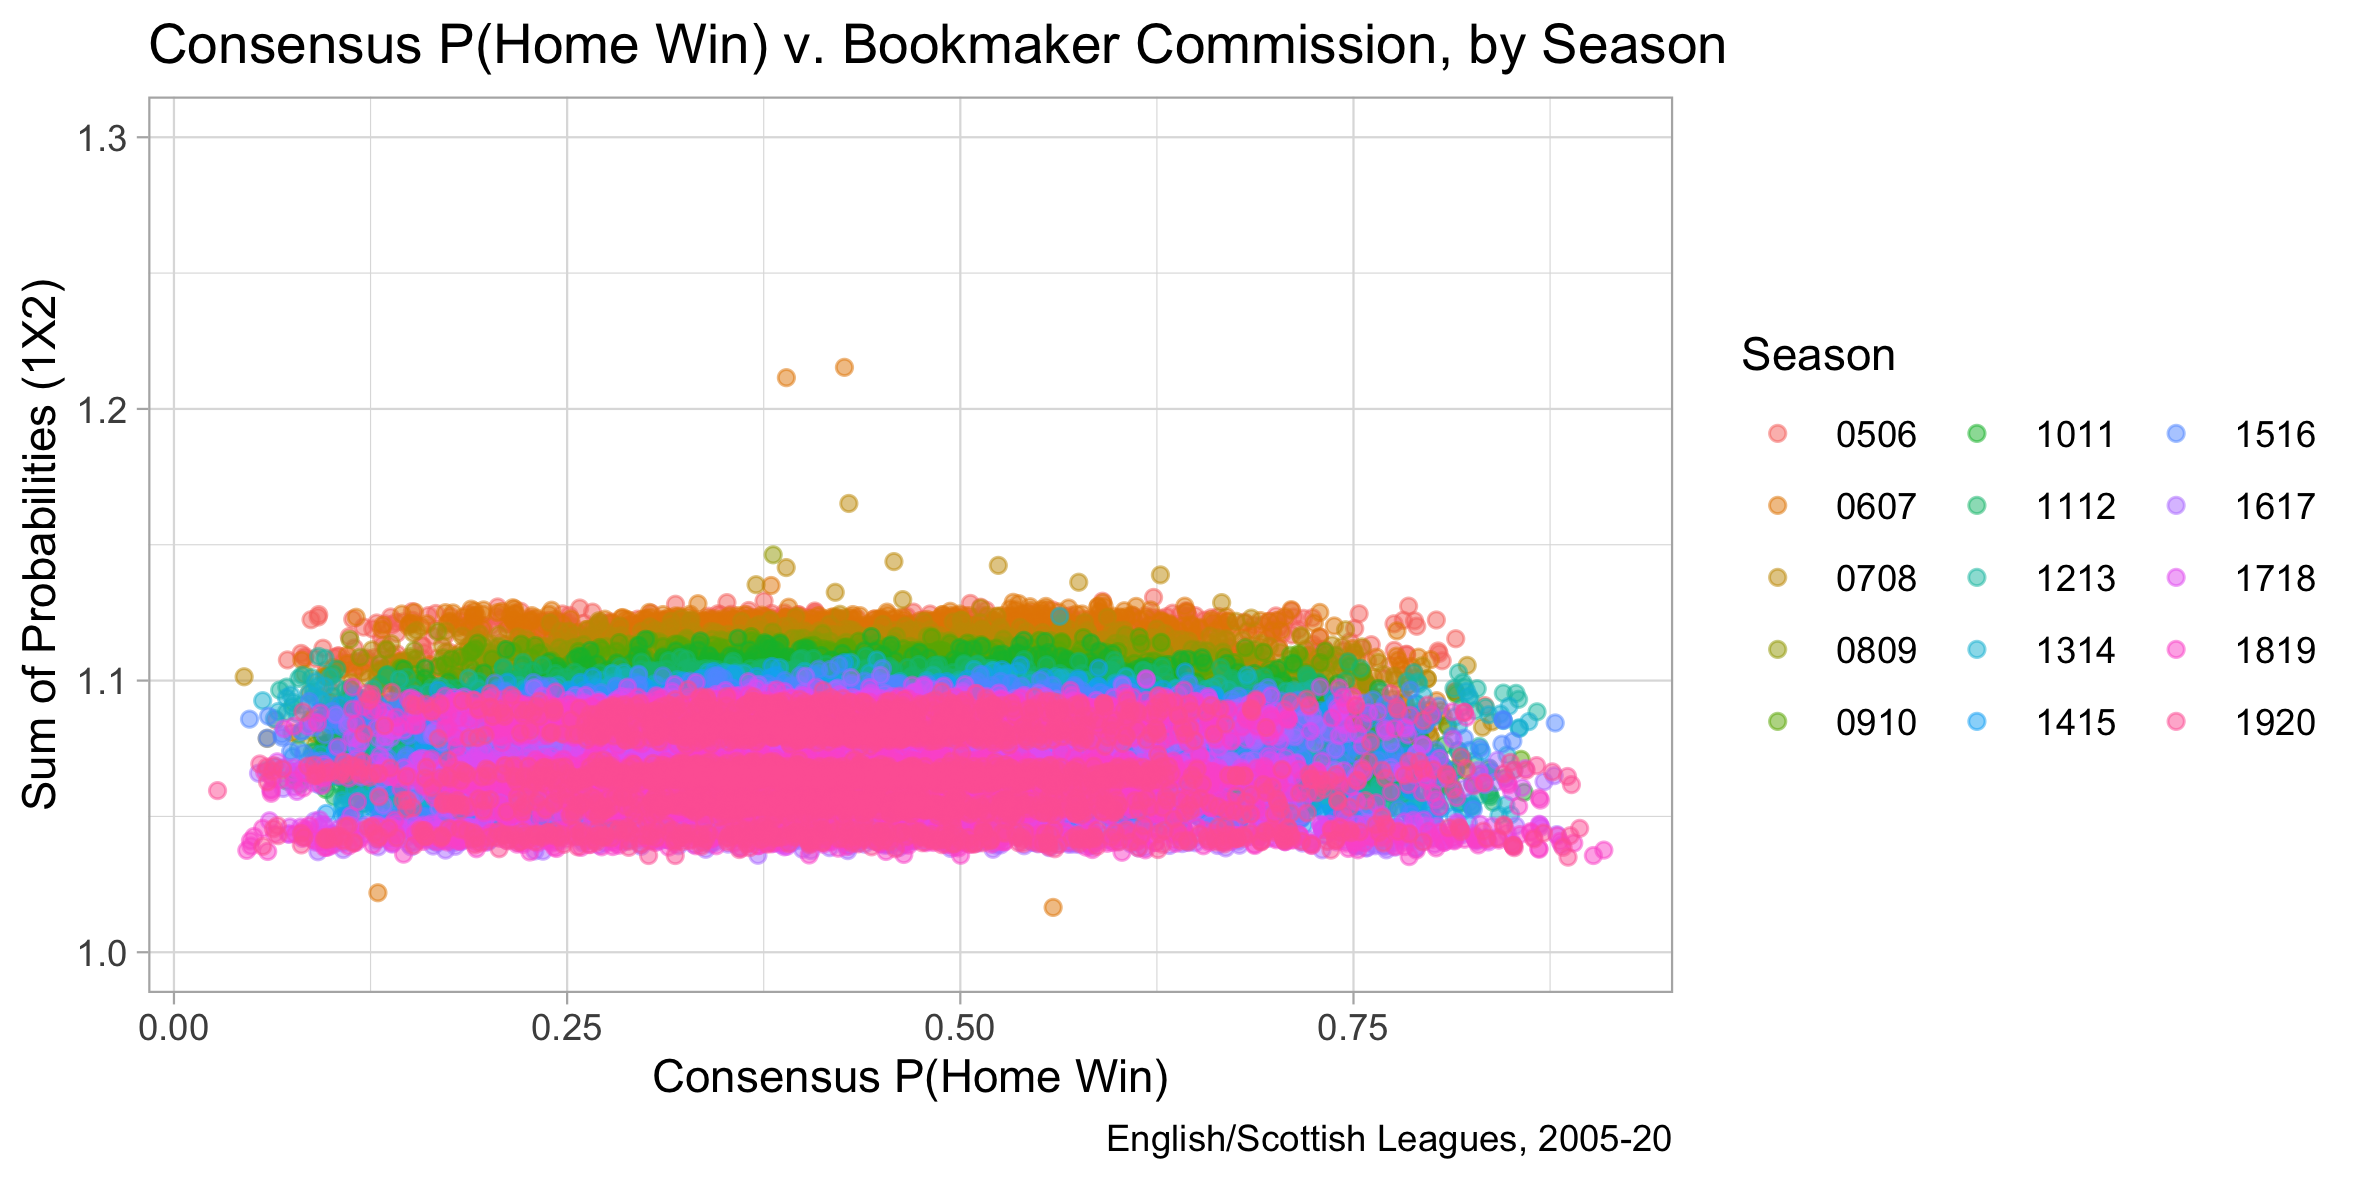
\includegraphics[width=0.9\textwidth]{ensco_14b_overround_ot_s.png}  
		\caption{The overround in the 1X2 market vs. $\mathbb{P}_{\textrm{cons}}$(1X2 Home Win), split by season.}\label{FIG:02_05b_overround1x2_season}
\end{center}\end{figure} \pagebreak

\begin{figure}[h!]\begin{center}
		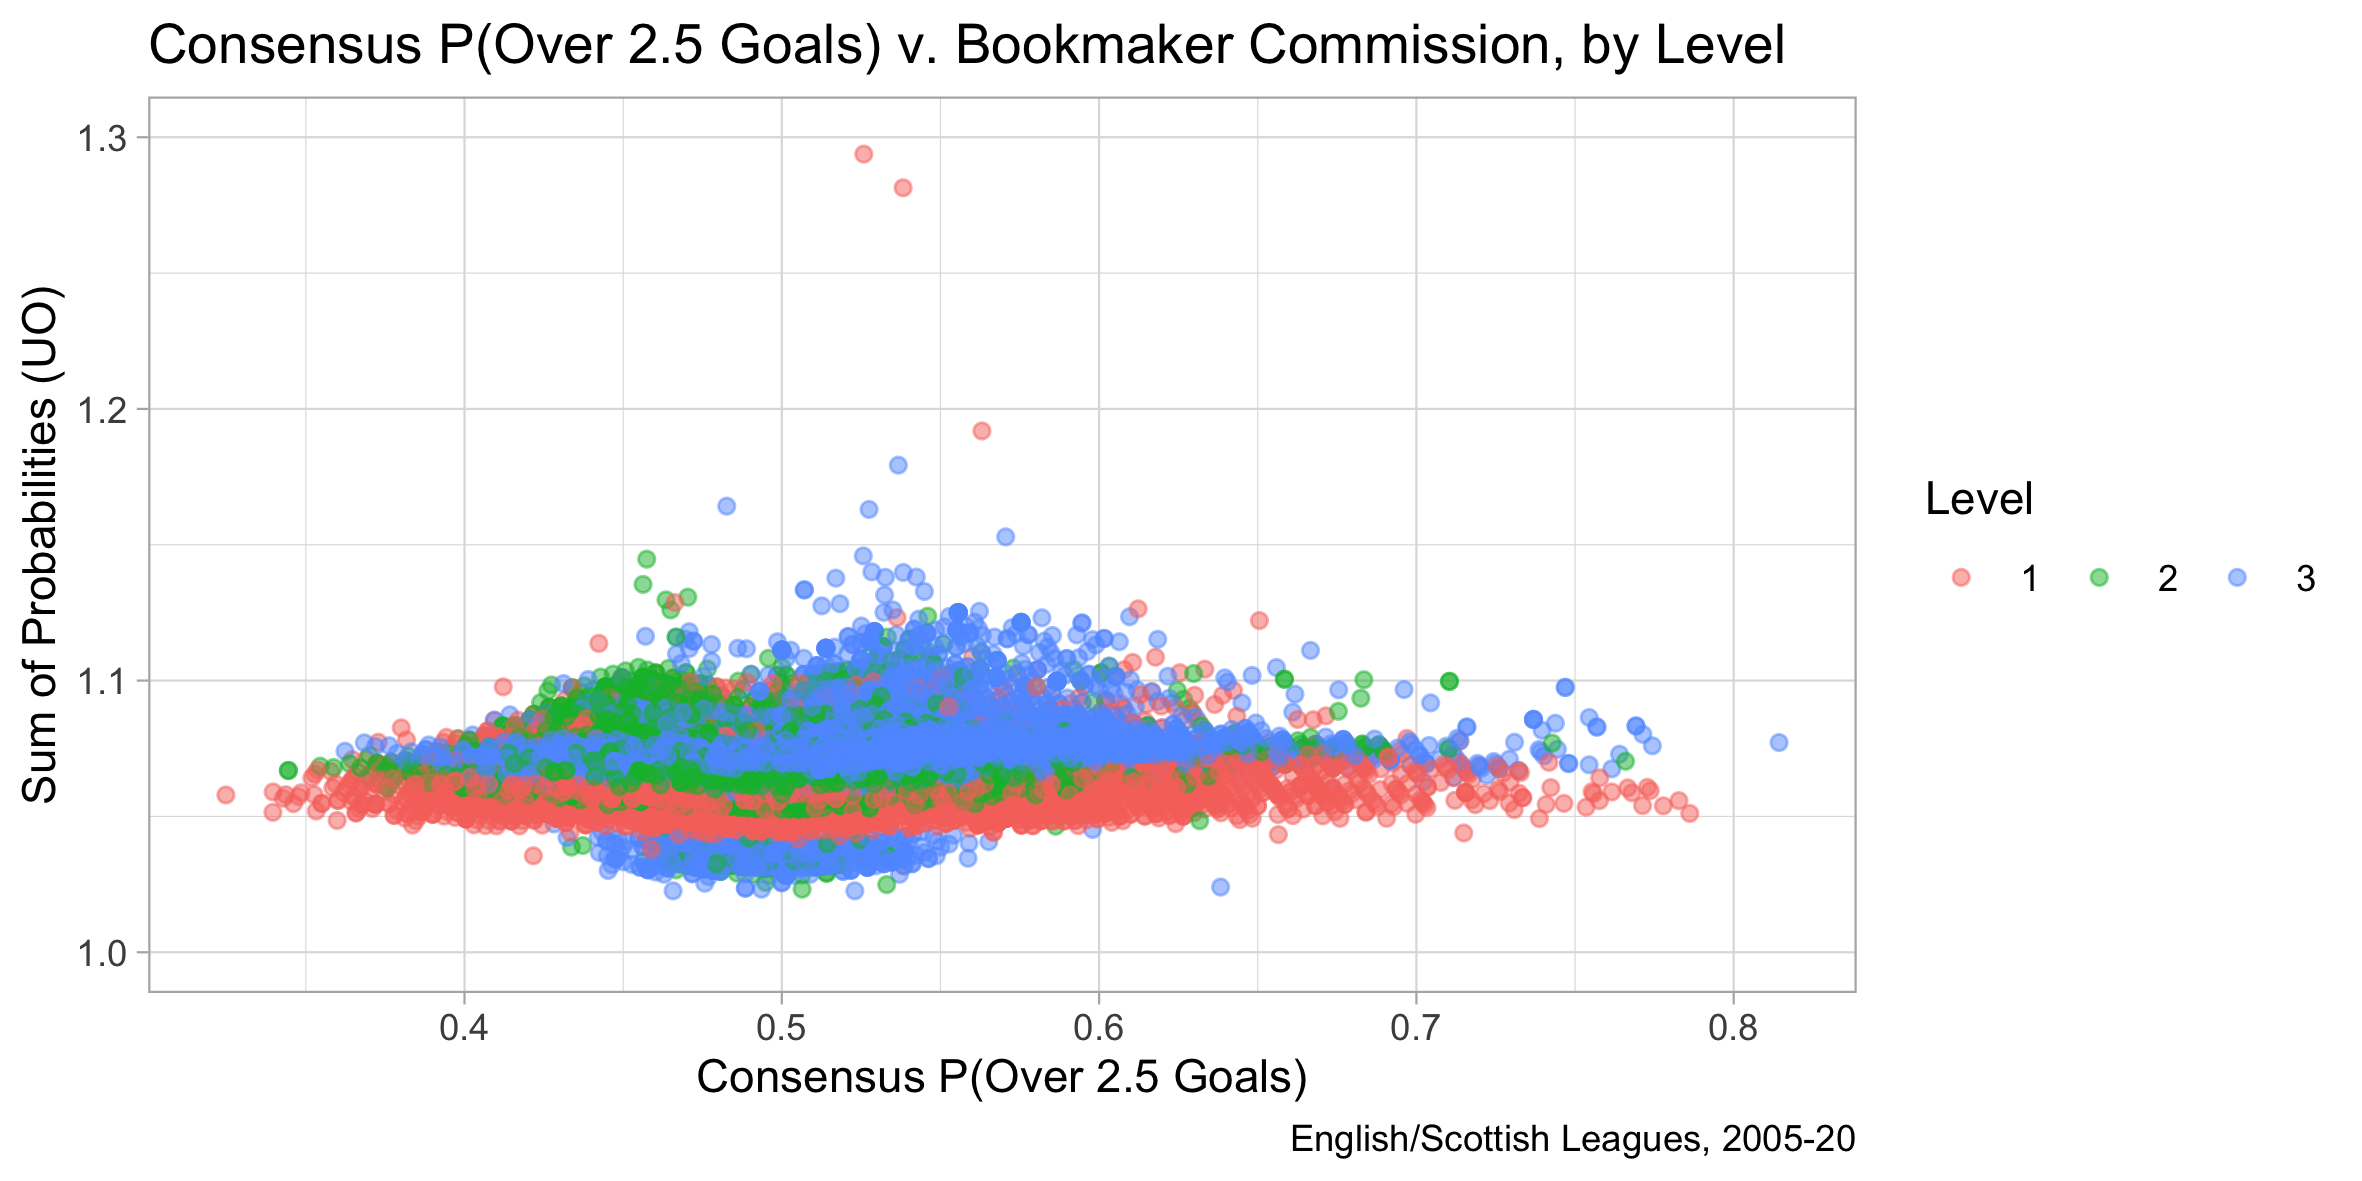
\includegraphics[width=0.9\textwidth]{ensco_14c_overround_uo_l.png}  
		\caption{The overround in the UO market vs. $\mathbb{P}_{\textrm{cons}}$(Over 2.5 Goals), split by level.}\label{FIG:02_06a_overrounduo_level}
\end{center}\end{figure}
\begin{figure}[h!]\begin{center}
		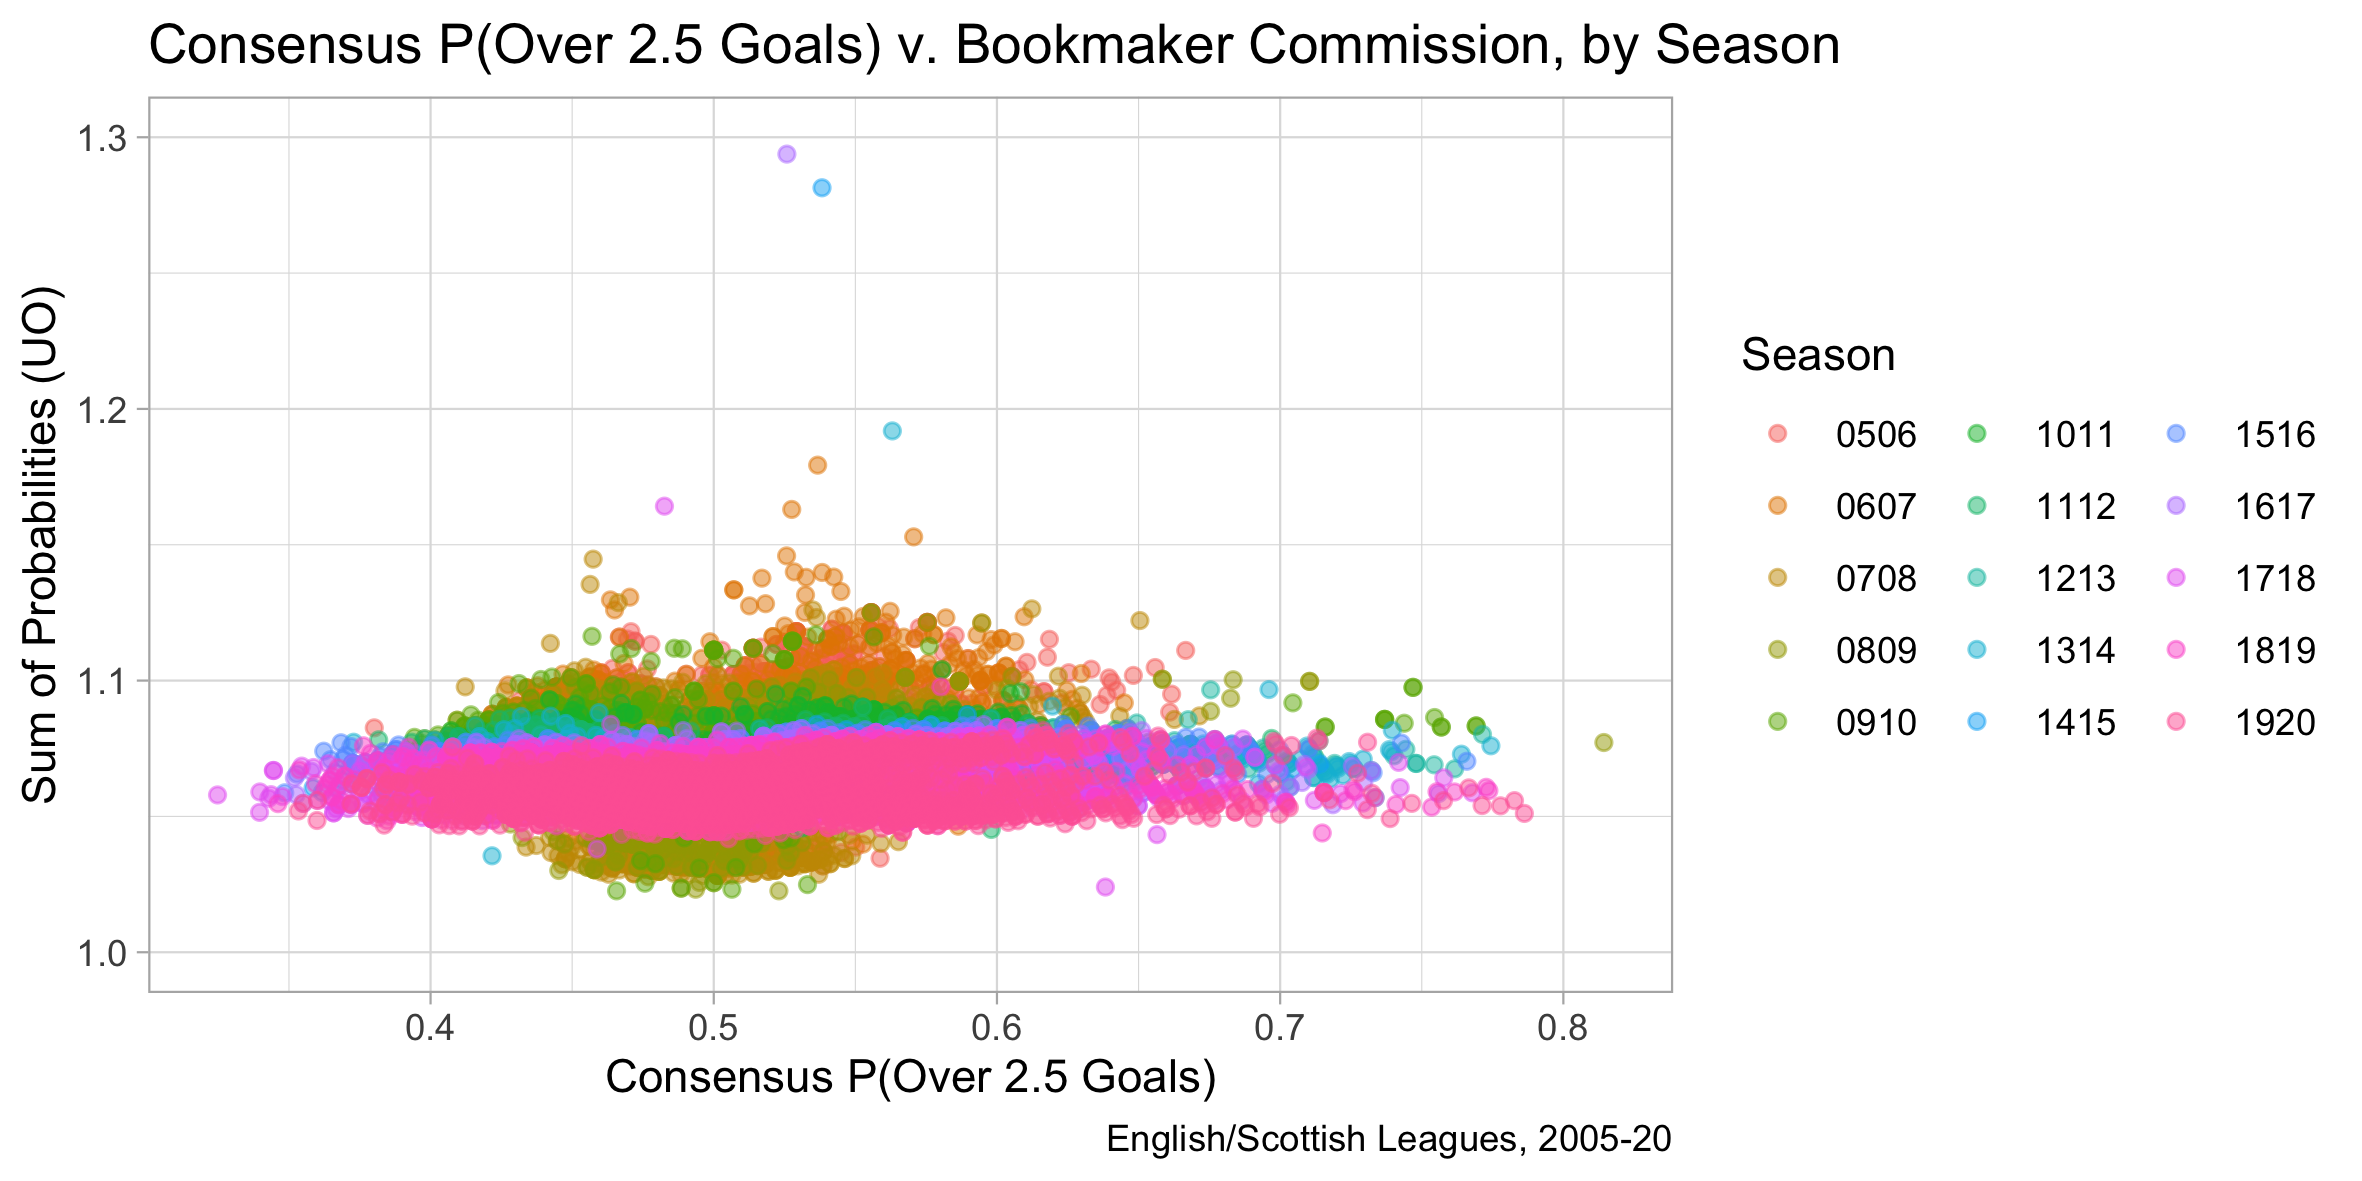
\includegraphics[width=0.9\textwidth]{ensco_14d_overround_uo_s.png}  
		\caption{The overround in the UO market vs. $\mathbb{P}_{\textrm{cons}}$(Over 2.5 Goals), split by season.}\label{FIG:02_06b_overrounduo_season}
\end{center}\end{figure} \pagebreak

\begin{figure}[h!]\begin{center}
		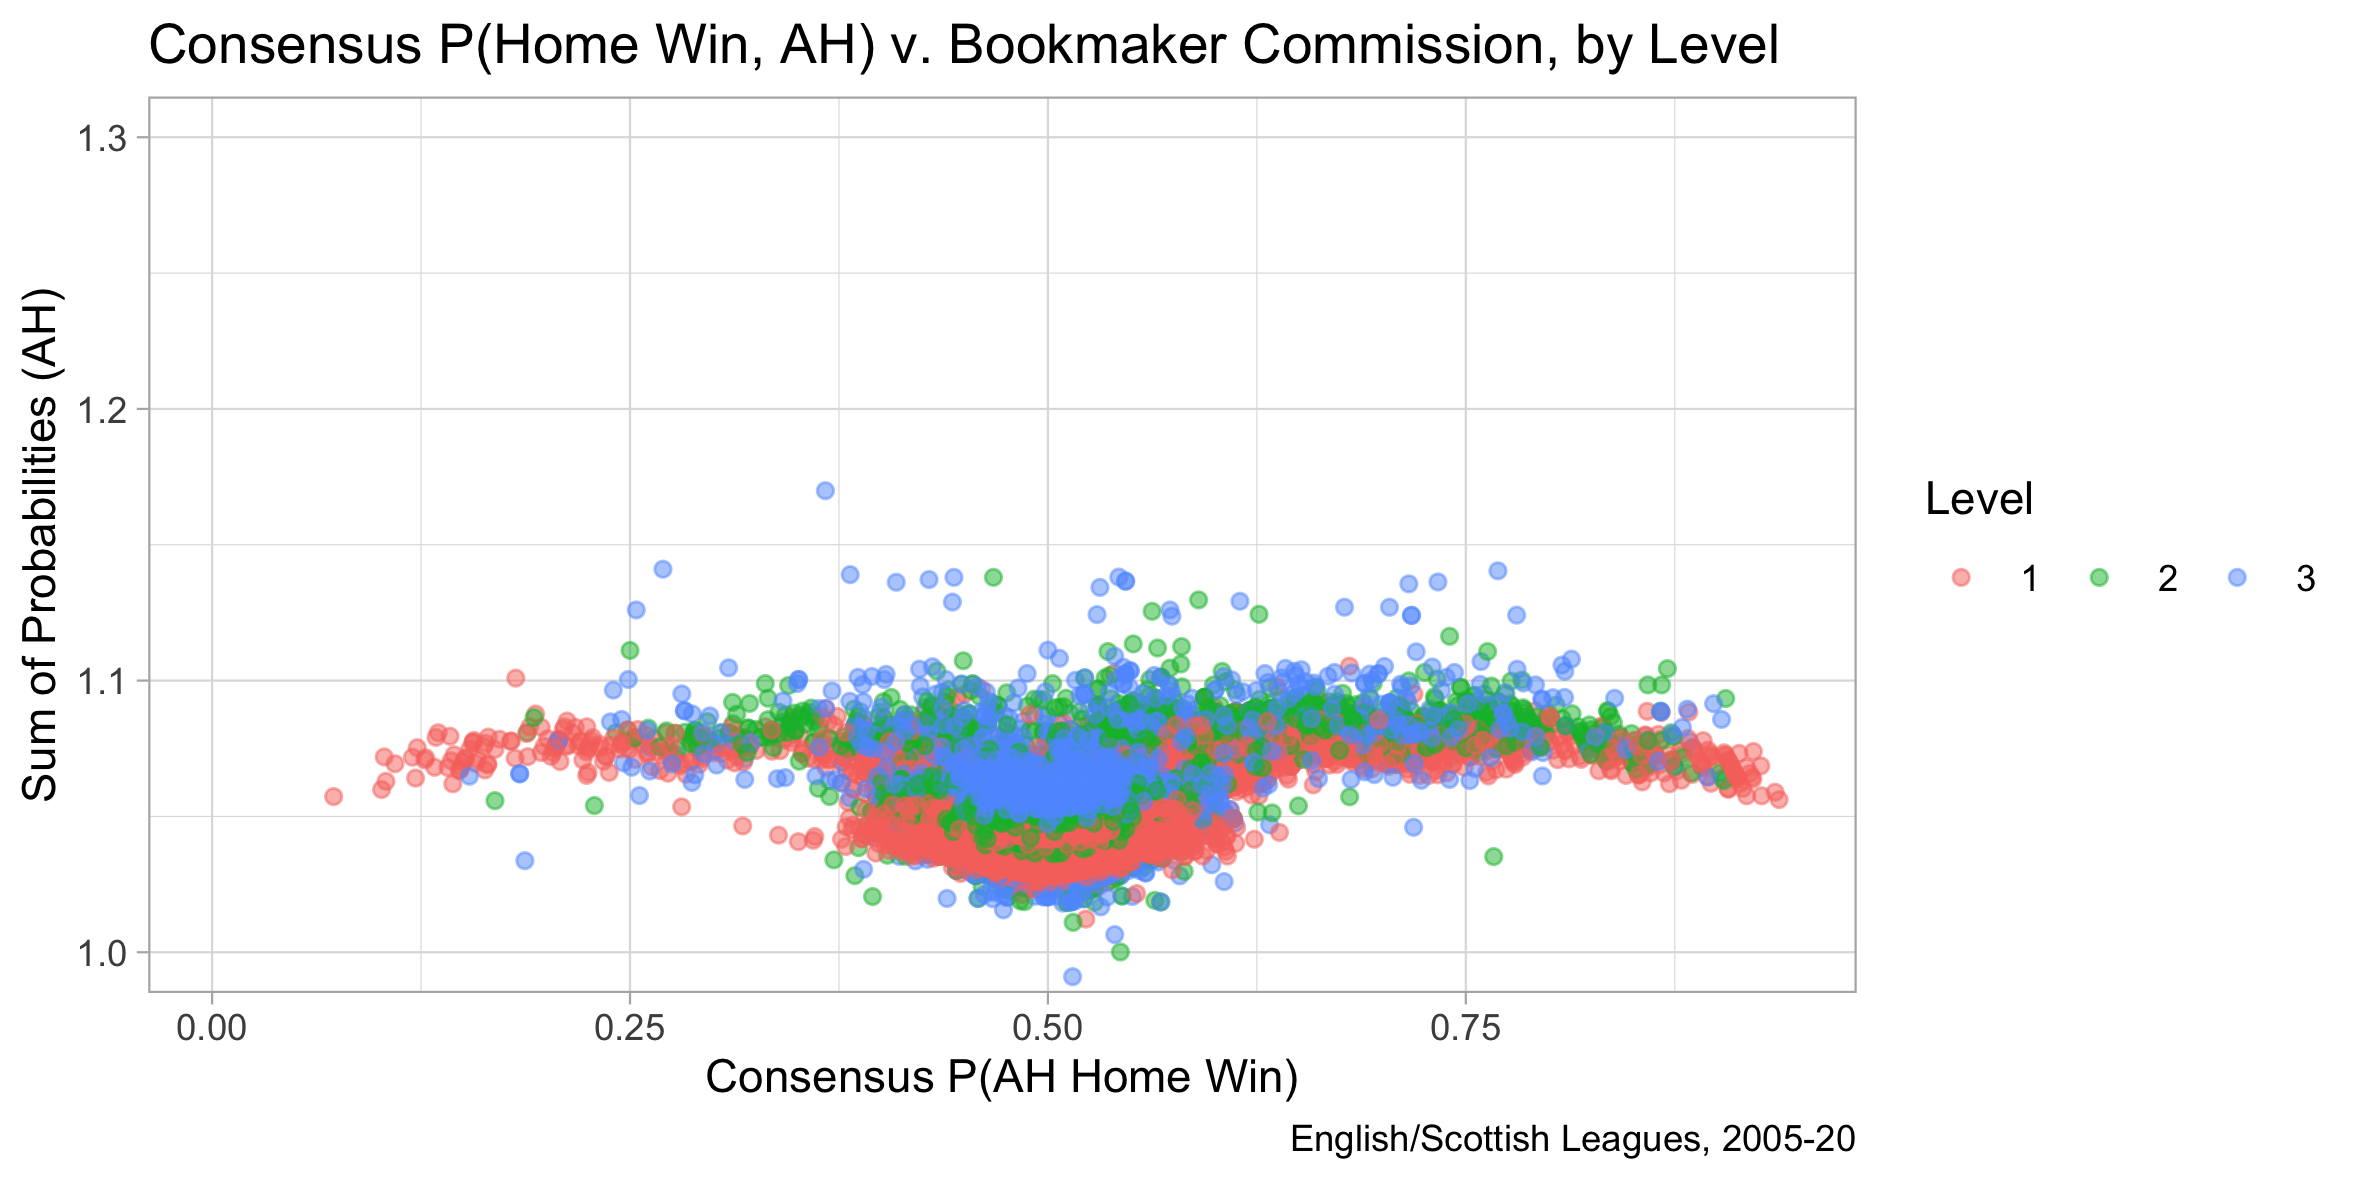
\includegraphics[width=0.9\textwidth]{ensco_14e_overround_ah_l.png}  
		\caption{The overround in the AH market vs. $\mathbb{P}_{\textrm{cons}}$(AH Home Win), split by level.}\label{FIG:02_07a_overroundah_level}
\end{center}\end{figure}
\begin{figure}[h!]\begin{center}
		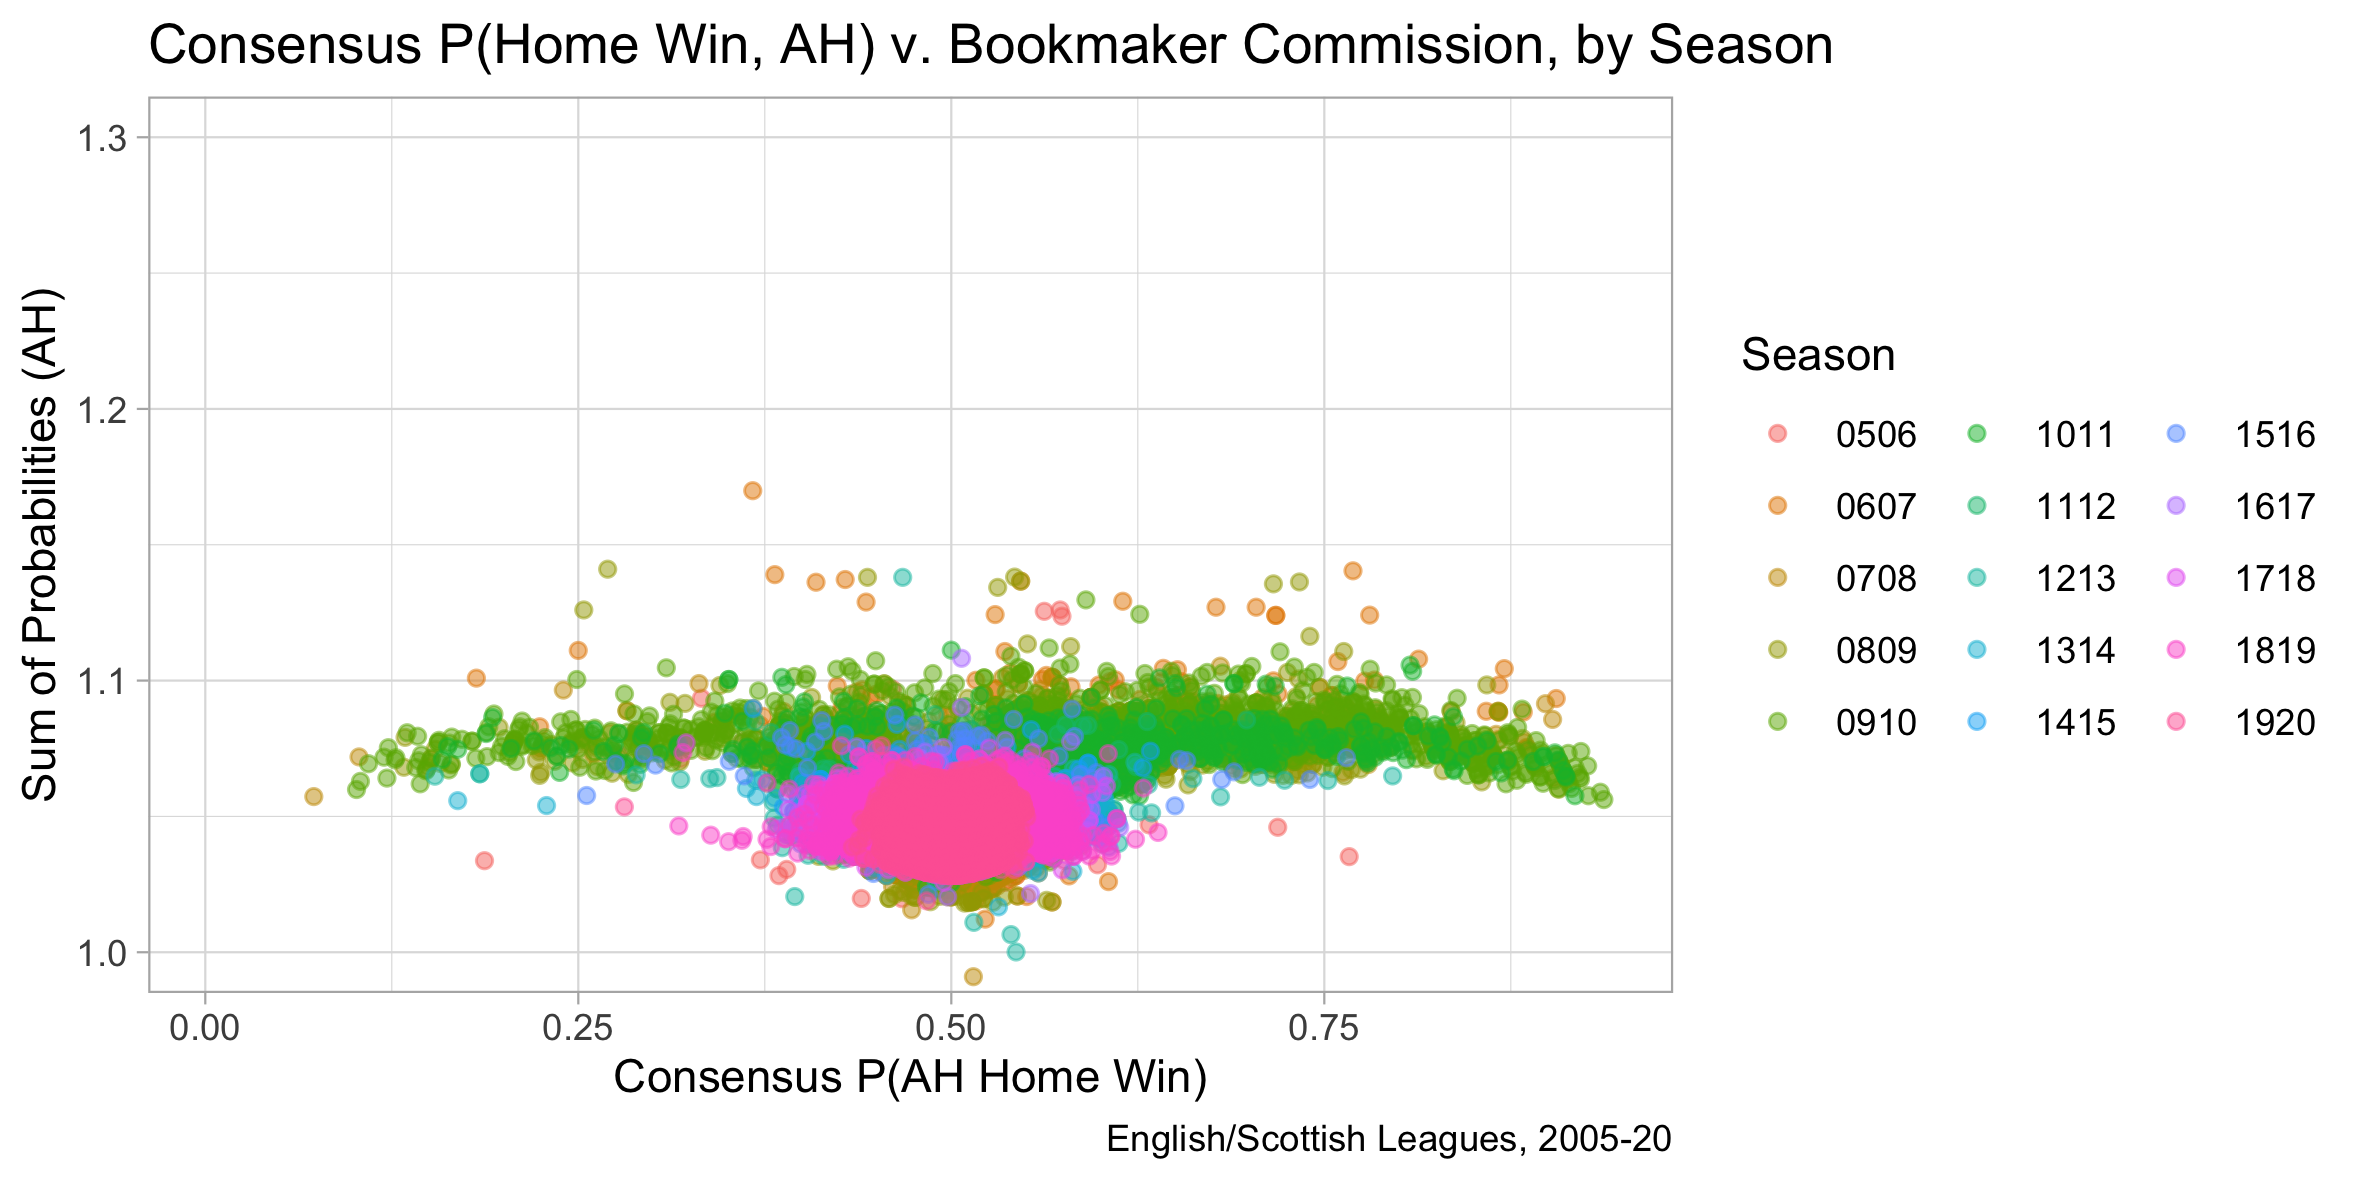
\includegraphics[width=0.8\textwidth]{ensco_14f_overround_ah_s.png}  
		\caption{The overround in the AH market vs. $\mathbb{P}_{\textrm{cons}}$(AH Home Win), split by season.}\label{FIG:02_7b_overroundah_season}
\end{center}\end{figure}\pagebreak


\section{Conclusion} \label{sec:enscoconc}
In this section, it has been found that across the English \& Scottish football league pyramids, bookmakers are most accurate in the 1X2 market (excluding performance on Draws), followed by the Asian Handicap market, with poor accuracy in the Under/Over 2.5 Goals market, however, the bookmaker accuracy is in fact decreasing in the AH market, and increasing in the UO market.  1X2 odds are, surprisingly, more accurate in Level 3---the lower leagues involving semi-professional sides---than in Level 2---wholly professional lower leagues; performance in Level 1 was greater than all other levels. Finally, in Section~\ref{sec:overround}, it has shown the bookmaker commission is highest in the 1X2 market, highest in lower levels, and is reducing over time. 

\begin{center}\noindent\rule{0.5\textwidth}{0.6pt}\end{center}

In Chapter~\ref{ch:model}, findings from Chapters~\ref{ch:elite} and \ref{ch:ensco} are applied in the creation of a proposed algorithm to place bets in an attempt to use bookmaker accuracy to turn a profit.


\chapter[A Proposed Betting Algorithm]{A proposed algorithm for placing bets.}\label{ch:model}

In this chapter, findings from Chapters~\ref{ch:elite} and \ref{ch:ensco} will be applied to attempt to \textit{beat the bookies} with their own odds, by accepting bookmaker accuracy is high.

\section{The Algorithm}\label{sec:method}

The function in Equation~\ref{eq:betscheme} is used to choose whether or not to, and how much to, bet in the 1X2 and Asian Handicap markets (measured in arbitrary units) on match $i$, market $m$, denoted as $B_{m,i}$. These markets are chosen as it was found in Chapters~\ref{ch:elite} and \ref{ch:ensco} that these show high levels of bookmaker accuracy. Despite the decreasing trend of accuracy in the AH market (Section~\ref{sec:comparingseasonsensco}) this algorithm is applied on the seasons considered throughout the project: 2005/06 until 2019/20, and as such, this market is chosen. The algorithm is designed to be able to be applied to any market, however, and can easily be adapted to place bets on the Under/Over 2.5 Goals market, or any other offered by bookmakers. The function is based on the consensus probability of the event $p_{m,i}$, where $\mu_m$ is the market mean and $\sigma_m$ is the market standard deviation, both of which are calculated up to and including the match $i$. This is more formally written in Algorithm~\ref{alg:placingbets}, where $p$ is the set of all consensus probabilities in the market of interest; $n$ the number of matches in the `information gathering' phase; $N$ the total number of matches in the dataset; $m$ the market chosen (for example, the 1X2 Home Win market).

\begin{equation}\label{eq:betscheme}
B_{m,i}(p_{m,i}, \mu_m, \sigma_m) = 
\begin{cases}
p_{m,i} < \mu_m + 0.5\sigma_m & B_{m,i} = 0 \\
\mu_m + 0.5\sigma_{m} \le p_{m,i} < \mu_m + \sigma_m & B_{m,i} = 1\\
\mu_m + \sigma_{m} \le p_{m,i} < \mu_m + 1.5\sigma_m & B_{m,i} = 2\\
\mu_m + 1.5\sigma_{m} \le p_{m,i}  & B_{m,i} = 3
\end{cases}
\end{equation}


\begin{algorithm}[h!] % Placing Bets 
	\caption{A proposed algorithm for placing bets.}\label{alg:placingbets}
	\begin{algorithmic}[1]
		\Function{bet }{$p;\ n;\ N;\ m$}
		\State $\mu_{n} \leftarrow$ mean $\mathbb{P}_{\textrm{cons}}$(Home Win, matches 1:$n$) \Comment{05/06 season data}
		\State $\sigma_{n} \leftarrow$ std dev $\mathbb{P}_{\textrm{cons}}$(Home Win, matches 1:$n$)
		\State $B_{i} \leftarrow 0$ \Comment{The placed bets}
		\State $i \leftarrow n$
		\While {$i \le N$}
		\State $\mu_{i} \leftarrow$ mean $\mathbb{P}_{\textrm{cons}}$(Home Win, matches 1:$i$) \Comment{Update $\mu$ and $\sigma$}
		\State $\sigma_{i} \leftarrow$ std dev $\mathbb{P}_{\textrm{cons}}$(Home Win, matches 1:$i$)
		\If {$p_{i} > \mu_{i} + 0.5\times\sigma_{i}$}
		\If {$p_{i} \le \mu_{i} + \sigma_{i}$}
		\State $B_i\leftarrow1$
		\ElsIf {$p_i > \mu_i + \sigma_i$ \textbf{and} $p_i \le \mu_i + 1.5\times\sigma_i$}
		\State $B_i\leftarrow2$
		\Else \Comment{$p_i > \mu_i + 1.5\times\sigma_i$}
		\State $B_i\leftarrow3$
		\EndIf
		\Else \Comment{$p_i \le \mu_i + 0.5\times\sigma_i$}
		\State $B_i\leftarrow0$
		\EndIf
		\State $i\leftarrow i+1$ \Comment{Iteration step}
		\EndWhile
		\State \Return $B_i$ \Comment{Repeat for all markets}
		\EndFunction
	\end{algorithmic}
\end{algorithm}

More is staked on probabilities further above the mean, as these will have lower odds, and thus, lower winnings, though the chance of the event occurring is higher. Doing it on the number of standard deviations away allows for different variances across the markets (it was found, for example, that the AH market varied less than the 1X2 market; Section~\ref{sec:enscoeda}), though the numbers of standard deviations away is an arbitrary choice. This is applied to the entire dataset considered in the project: all markets in the \textit{elite} European leagues\footnote{Analysis wasn't conducted on the Asian Handicap market in the \textit{elite} dataset, meaning the AH bets placed on those matches will be `blind' and thus, more fitting to a real-life scenario.} and the English \& Scottish league pyramids. This is a total of $N = 75086$ matches with $n=5012$ matches in the 2005/06 season (`information gathering', relating to lines 2--4 of the algorithm).

The algorithm is ran in R using the code below. (\textsc{n.b.}, before this is carried out, the data is first read in, using the same method as in Chapters~\ref{ch:elite} and \ref{ch:ensco}, calling the dataframe \lstinline|matches|). Statistics for the number of bets, and units staked, is given in Table~\ref{tab:betstats}.

\begin{lstlisting}
matches$OTHomeBet <- with(matches, 0); matches$OTAwayBet <- with(matches, 0)
matches$AHHomeBet <- with(matches, 0); matches$AHAwayBet <- with(matches, 0)

#Initial Bounds :-
matches0506 <- matches[matches$Season == '0506',]
mu.oth <- mean(matches0506$OT.HProb); sd.oth <- sd(matches0506$OT.HProb)
mu.ota <- mean(matches0506$OT.AProb); sd.ota <- sd(matches0506$OT.AProb)
mu.ahh <- mean(matches0506$AH.HProb); sd.ahh <- sd(matches0506$AH.HProb)
mu.aha <- mean(matches0506$AH.AProb); sd.aha <- sd(matches0506$AH.AProb)
n <- nrow(matches[matches$Season == "0506",]); N <- nrow(matches)
#Placing Bets:-
for (i in n:N){
	#Update the mean and std dev's with our new information
	mu.oth <- mean(matches$OT.HProb[1:i]); sd.oth <- sd(matches$OT.HProb[1:i])
	mu.ota <- mean(matches$OT.AProb[1:i]); sd.ota <- sd(matches$OT.AProb[1:i])
	mu.ahh <- mean(matches$AH.HProb[1:i]); sd.ahh <- sd(matches$AH.HProb[1:i])
	mu.aha <- mean(matches$AH.AProb[1:i]); sd.aha <- sd(matches$AH.AProb[1:i])
	#Do we bet on Home Win (1X2)?
	if (matches$OT.HProb[i] > mu.oth + 0.5*sd.oth){
		if (matches$OT.HProb[i] <= mu.oth + sd.oth){matches$OTHomeBet[i] <- 1}
		else if (matches$OT.HProb[i] > mu.oth + sd.oth & matches$OT.HProb[i] <= mu.oth + 1.5*sd.oth){matches$OTHomeBet[i] <- 2}
		else {matches$OTHomeBet[i] <- 3}}
	else {matches$OTHomeBet[i] <- 0}
	#Do we bet on Away Win (1X2)?
	if (matches$OT.AProb[i] > mu.ota + 0.5*sd.ota){
		if (matches$OT.AProb[i] <= mu.ota + sd.ota){matches$OTAwayBet[i] <- 1}
		else if (matches$OT.AProb[i] > mu.ota + sd.ota & matches$OT.AProb[i] <= mu.ota + 1.5*sd.ota){matches$OTAwayBet[i] <- 2}
		else {matches$OTAwayBet[i] <- 3}}
	else {matches$OTAwayBet[i] <- 0}
	#Do we bet on Home Win (AH)?
	if (matches$AH.HProb[i] > mu.ahh + 0.5*sd.ahh){
		if (matches$AH.HProb[i] <= mu.ahh + sd.ahh){matches$AHHomeBet[i] <- 1}
		else if (matches$AH.HProb[i] > mu.ahh + sd.ahh & matches$AH.HProb[i] <= mu.ahh + 1.5*sd.ahh){matches$AHHomeBet[i] <- 2}
		else {matches$AHHomeBet[i] <- 3}}
	else {matches$AHHomeBet[i] <- 0}
	#Do we bet on Away Win (AH)?
	if (matches$AH.AProb[i] > mu.aha + 0.5*sd.aha){
		if (matches$AH.AProb[i] <= mu.aha + sd.aha){matches$AHAwayBet[i] <- 1}
		else if (matches$AH.AProb[i] > mu.aha + sd.aha & matches$AH.AProb[i] <= mu.aha + 1.5*sd.aha){matches$AHAwayBet[i] <- 2}
		else {matches$AHAwayBet[i] <- 3}}
	else {matches$AHAwayBet[i] <- 0}
}
\end{lstlisting} 

\begin{table}[h!]\begin{center}\begin{tabular}{c||cc|cc}
					   & \multicolumn{4}{|c}{\textit{Market}} \\
					   & \multicolumn{2}{|c}{1X2} & \multicolumn{2}{|c}{AH} \\
	\textit{Units Bet} & H Win & A Win & H Win & A Win \\ \hline\hline
	0 & 55352 & 55068 & 63348 & 55432 \\ \hdashline
	1 & 8664 & 8880 & 6798 & 14381 \\ 
	2 & 4951 & 4717 & 2011 & 3847 \\
	3 & 6119 & 6421 & 2929 & 1426 \\ \hline \hline
	\textit{Total Bets} & 19734 & 20018 & 11738 & 19654 \\ 
	\textit{Stake}      & 36923 & 37577 & 19607& 26353
\end{tabular}\end{center}\caption{The total number of bets placed, in units, across each market in the proposed algorithm.}\label{tab:betstats}
\end{table}

Running the code generates four new columns: \lstinline|OTHomeBet|, \lstinline|OTAwayBet|, \lstinline|AHHomeBet|, and \lstinline|AHAwayBet| representing $B_{i,\textsc{oth}}$, $B_{i,\textsc{ota}}$, $B_{i,\textsc{ahh}}$, $B_{i,\textsc{aha}}$ respectively.\footnote{The 1X2 market is represented with \lstinline|ot| and the Asian Handicap with \lstinline|ah|, followed by \lstinline|h| or \lstinline|a| for the Home or Away Win market.} Each entry is equal to either 0, 1, 2, or 3. 

\subsection{Motivation}\label{ssec:motivationofmethod}
\citeauthor{kaunitz17} (\citeyear{kaunitz17}) created a high-performing method that made a 3.5\% return on 56,435 bets had an accuracy (proportion of bets won) of 44.4\%. The paper found mispriced odds by comparing the maximum odds available with the consensus bookmaker odds. If the maximum was sufficiently high (\textsc{i.e.}, the consensus probability sufficiently low), a bet (by comparison, worth one unit of the bets placed in this algorithm) was placed. The data used was over a similar timeframe: from 2005 to 2015, but over a much larger set of matches (479,440 matches across 818 leagues). Whilst this method is profitable, individual bettors without the help of methods to deal with large amounts of data (such as data scraping) and methods to find maximum odds and consensus odds will be unable to run this (for example, the \url{football-data.co.uk} data is uploaded after the matches take place\footnote{Odds are collected, for weekend games, on Friday afternoons, as mentioned in Section~\ref{ssec:data}, but the final \lstinline|.csv| files contain match statistics only available after the matches take place.} so a bettor would have to collect the information themselves). A bettor would be able to follow the algorithm proposed in this project (a bookmaker, or range of bookmakers, would need to be chosen, and the means/standard deviations can be calculated weekly, monthly, or even by-season). The aim is to create a simpler method that bettors can use based on the findings laid out in this paper.

\subsection[Alternate Method]{An Alternate Method Excluding Poor Performing Leagues}\label{ssec:alternatemethod}

In addition to finding that the overall bookmaker accuracy was high in the 1X2 Home Win and Away Win, and Asian Handicap markets, two of the \textit{elite} leagues and one of the levels was found to have worse bookmaker performance: the French Ligue Une, German Bundesliga, and the English \& Scottish Level 2 (English Leagues One and Two; Scottish Championship). The \textit{alternate} method used will follow the same algorithm, with the exclusion of these leagues. The bets are placed using the code below.

\begin{lstlisting}
matches$OTHomeBet.alt <- with(matches, OTHomeBet)
matches$OTAwayBet.alt <- with(matches, OTAwayBet)
matches$AHHomeBet.alt <- with(matches, AHHomeBet)
matches$AHAwayBet.alt <- with(matches, AHAwayBet)

#Removing bets placed in France, Germany and Level 2, Eng/Sco:-
for (i in 1:N){
	if (matches$Div[i] %in% c("D1", "F1", "E2", "E3", "SC1")){
		matches$OTHomeBet.alt[i] <- 0
		matches$OTAwayBet.alt[i] <- 0
		matches$AHHomeBet.alt[i] <- 0
		matches$AHAwayBet.alt[i] <- 0
	}
}
\end{lstlisting}

Naturally, the number of bets (and thus, the stake) will be lower in this method; to compare, the accuracy percentage is used, that is, the number of correct bets divided by the total number of bets; and the proportion: the winnings divided by the stake. 

\section{Computing the Winnings} \label{sec:winnings}

Once the bets have been placed, the winnings must be found, using the original bookmaker odds offered. Algorithms~\ref{alg:winningsot} and \ref{alg:winningsah} are used to calculate the 1X2 and AH winnings respectively, assuming the Winning Probabilities code in Section~\ref{sec:enscoeda} has been ran. \vspace{3mm}

\begin{algorithm}
	\caption{An algorithm for computing the winnings from Algorithm~\ref{alg:placingbets} in the 1X2 market.} \label{alg:winningsot}
	\begin{algorithmic}[1]
		\Function{1X2Winnings }{$B_{i,m};\ O_{i,m};\ \textrm{FTR}_i$} \Comment{Assuming European odds}
		\State Set all winnings $\omega_{i,m} \leftarrow 0$
		\State Set market cumulative returns $\Omega_{i,m}\leftarrow 0$
		\State Initialise count, $i \leftarrow n+1$ \Comment{$n$ = 5012, ignore information gathering}
		\While {$i \le N$} \Comment{$N = 75086$}
		\If{$\textrm{FTR}_i$ = HomeWin}
		\State $\omega_{i, \textsc{oth}}\leftarrow (O_{i,\textsc{oth}} - 1)\times B_{i, \textsc{oth}}$ 
		\State $\omega_{i, \textsc{ota}}\leftarrow -B_{i, \textsc{ota}}$
		
		\ElsIf{$\textrm{FTR}_i$ = AwayWin}
		\State $\omega_{i, \textsc{oth}}\leftarrow -B_{i, \textsc{oth}}$
		\State $\omega_{i, \textsc{ota}}\leftarrow (O_{i,\textsc{ota}} - 1)\times B_{i, \textsc{ota}}$ 
		
		\Else \Comment{\textsc{i.e.}, a Draw}
		\State $\omega_{i, \textsc{oth}}\leftarrow -B_{i, \textsc{oth}}$
		\State $\omega_{i, \textsc{ota}}\leftarrow -B_{i, \textsc{ota}}$
		\EndIf
		\State $i\leftarrow i + 1$ \Comment{Iteration step}
		\State $\Omega_{i,\textsc{oth}} \leftarrow \Omega_{(i-1),\textsc{oth}} + \omega_{i,\textsc{oth}}$ \Comment{Update cumulative returns}
		\State $\Omega_{i,\textsc{ota}} \leftarrow \Omega_{(i-1),\textsc{ota}} + \omega_{i,\textsc{ota}}$
		\EndWhile
		\State\Return{$\Omega_{\textsc{oth}},\ \Omega_{\textsc{ota}}$}
		\EndFunction
	\end{algorithmic}
\end{algorithm}

\pagebreak

\begin{algorithm}
	\caption{An algorithm for computing the winnings from Algorithm~\ref{alg:placingbets} in the AH market.}\label{alg:winningsah}
	\begin{algorithmic}[1]		
		\Function{AHWinnings }{$B_{i,m};\ O_{i,m};\ \textrm{AHRes}_i$} \Comment{Assuming European odds}
		\State Set all winnings $\omega_{i,m} = 0$
		\State Set market cumulative returns $\Omega_{i,m}\leftarrow 0$
		\State Initialise count, $i \leftarrow n+1$ \Comment{$n$ and $N$ as before}
		\While {$i \le N$}
		\If{$\textrm{AHRes}_i$ = FullHomeWin}
		\State $\omega_{i, \textsc{ahh}}\leftarrow (O_{i,\textsc{ahh}} - 1)\times B_{i, \textsc{ahh}}$ 
		\State $\omega_{i, \textsc{aha}}\leftarrow -B_{i, \textsc{aha}}$
		
		\ElsIf{$\textrm{AHRes}_i$ = HalfHomeWin}
		\State $\omega_{i, \textsc{ahh}}\leftarrow (O_{i,\textsc{ahh}} - 1)\times 0.5 \times B_{i, \textsc{ahh}} - (0.5\times B_{i, \textsc{ahh}})$
		\State $\omega_{i, \textsc{aha}}\leftarrow -B_{i, \textsc{aha}}$
		
		\ElsIf{$\textrm{AHRes}_i$ = FullAwayWin}
		\State $\omega_{i, \textsc{ahh}}\leftarrow -B_{i, \textsc{ahh}}$
		\State $\omega_{i, \textsc{aha}}\leftarrow (O_{i,\textsc{aha}} - 1)\times B_{i, \textsc{aha}}$ 
		
		\ElsIf{$\textrm{AHRes}_i$ = HalfAwayWin}
		\State $\omega_{i, \textsc{ahh}}\leftarrow -B_{i, \textsc{ahh}}$
		\State $\omega_{i, \textsc{aha}}\leftarrow (O_{i,\textsc{aha}} - 1)\times 0.5 \times B_{i, \textsc{aha}} - (0.5\times B_{i, \textsc{aha}})$
		
		\Else \Comment{\textsc{i.e.}, a Voided Bet}
		\State $\omega_{i, \textsc{ahh}}\leftarrow 0$
		\State $\omega_{i, \textsc{aha}}\leftarrow 0$
		\EndIf
		\State $i\leftarrow i + 1$ \Comment{Iteration step}
		\State $\Omega_{i,\textsc{ahh}} \leftarrow \Omega_{(i-1),\textsc{ahh}} + \omega_{i,\textsc{ahh}}$ \Comment{Update cumulative returns}
		\State $\Omega_{i,\textsc{aha}} \leftarrow \Omega_{(i-1),\textsc{aha}} + \omega_{i,\textsc{aha}}$
		\EndWhile
		\State\Return{$\Omega_{\textsc{ahh}},\ \Omega_{\textsc{aha}}$}
		\EndFunction		
	\end{algorithmic}
\end{algorithm}

(\textsc{n.b.}, One may notice that one is subtracted from the odds offered, and wonder why. As mentioned in Section~\ref{sec:proboddsgambling}, the decimal (European) odds are defined with the stake included, and would therefore inflate the winnings reported. Strict winnings can be found using the fractional (British) odds, computed by subtracting one from the decimal odds. If fractional odds were inputted to the algorithm, these steps should be ignored.)

\pagebreak
\section{Results}\label{sec:modelresults}

In addition to running the algorithms in R, each match is assigned with an `index' by taking matches $n+1$ to $N$ and numbering them from 1 to $N-n$. The index is used to create a line plot of the cumulative winnings. This is shown in Figure~\ref{FIG:03_01_cumulativewinnings}, with a zoomed-in plot of the first 100 matches shown in Figure~\ref{FIG:03_02_cumulativewinnings100}.

\begin{figure}[p!]\begin{center}
	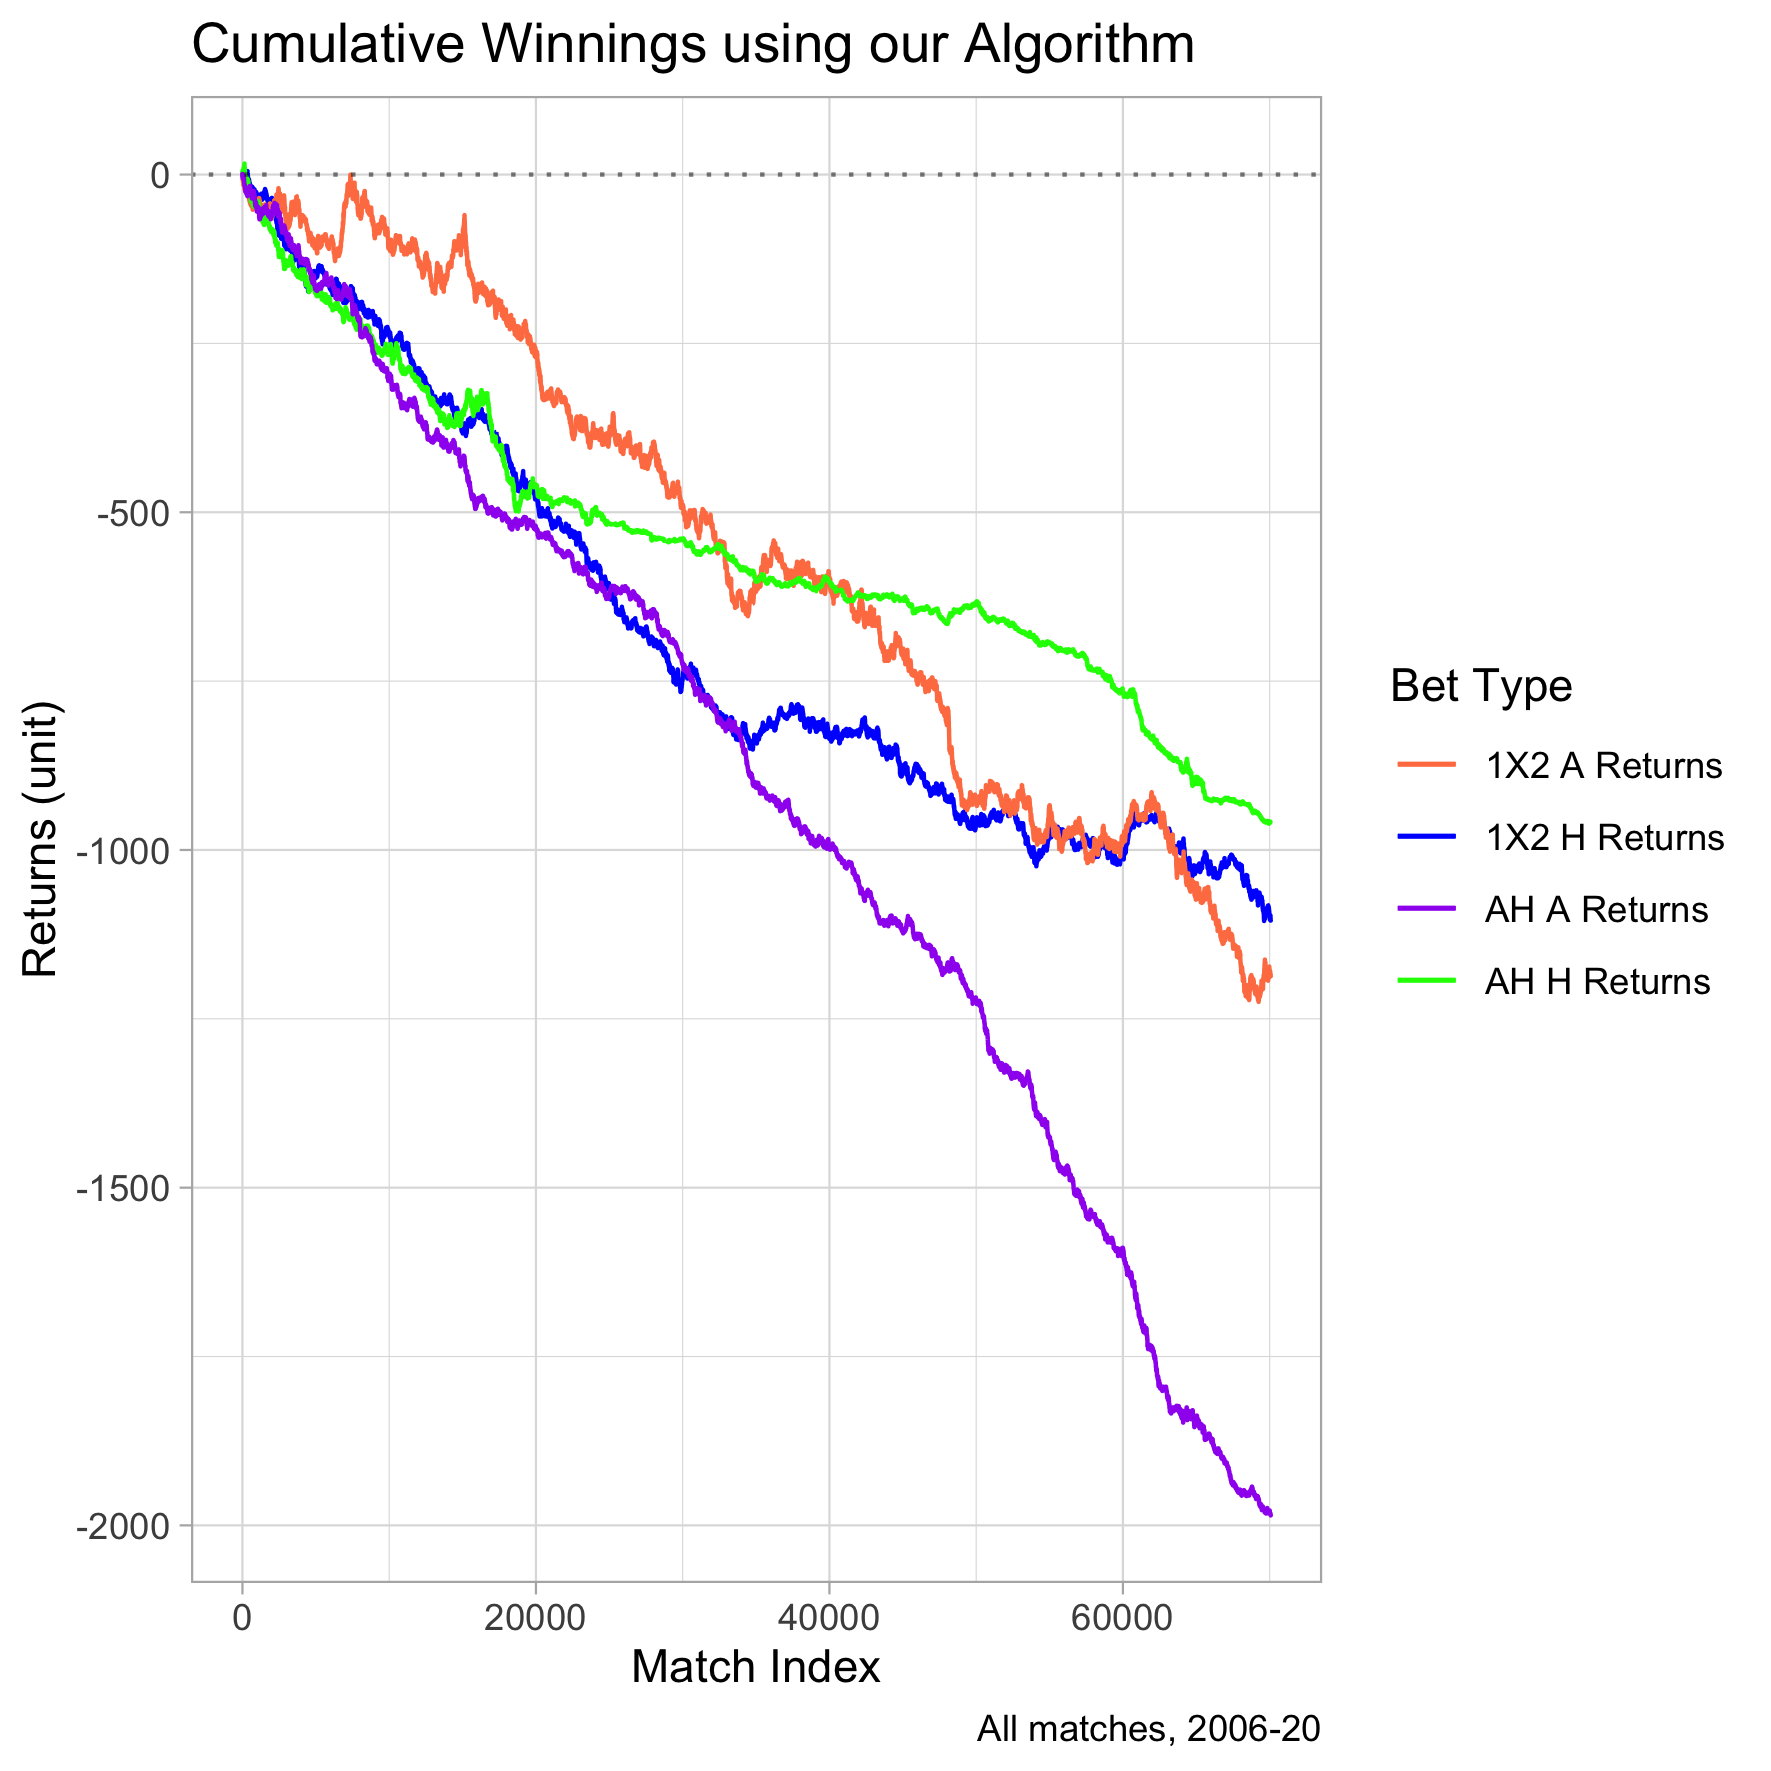
\includegraphics[width=\textwidth]{model_01.png}  
	\caption{A plot of the cumulative winnings of the proposed betting algorithm, split by market.}\label{FIG:03_01_cumulativewinnings}
\end{center}\end{figure}

\begin{figure}[h!]\begin{center}
	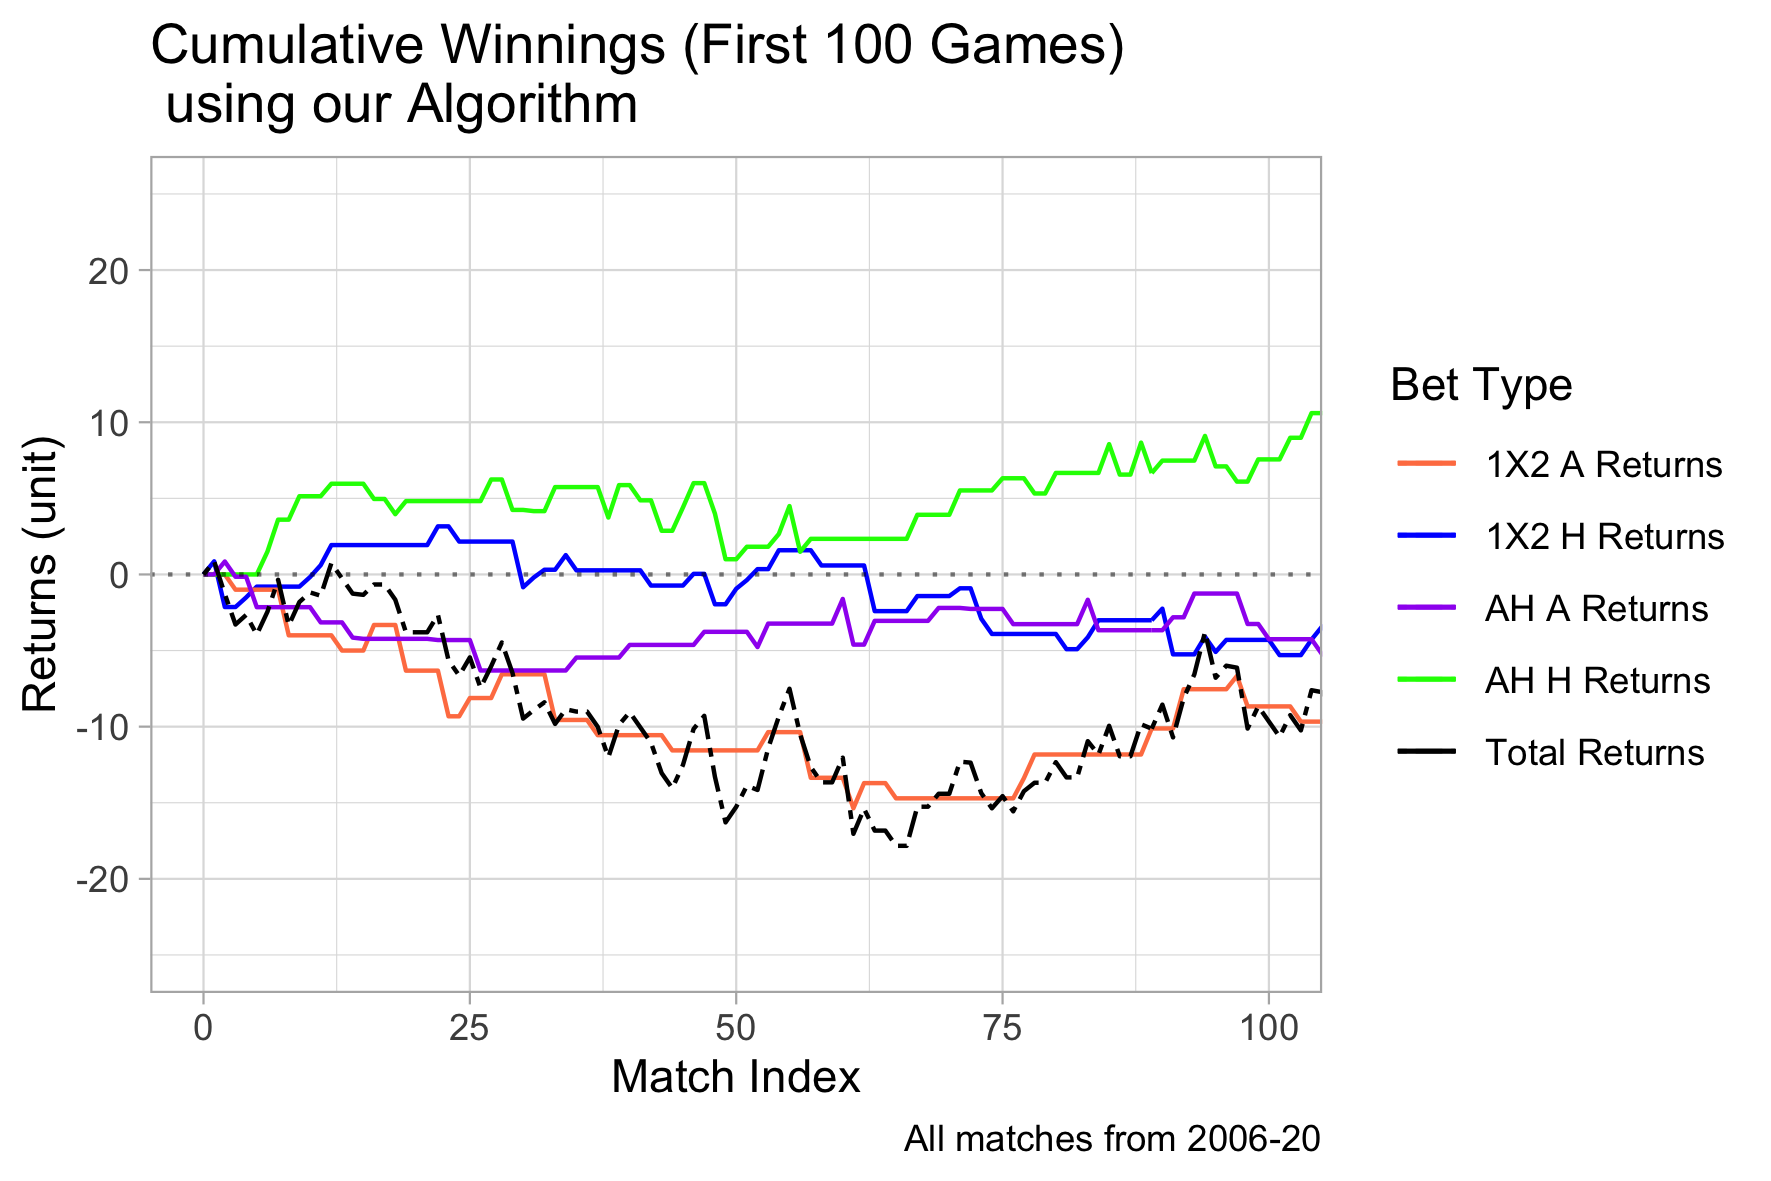
\includegraphics[width=0.8\textwidth]{model_02.png}  
	\caption{A zoomed in view of Figure~\ref{FIG:03_01_cumulativewinnings}, considering the first 100 matches.}\label{FIG:03_02_cumulativewinnings100}
\end{center}\end{figure}

The performance of the first 100 matches is not too bad, with the overall profit line hovering just below the $y=0$ line. The total winnings, however, show a rather conclusive loss. `Money' is lost in all four markets, with the biggest loss ($\approx 2,000$ units) in the Asian Handicap Away Win market. Full figures are in Table~\ref{tab:betaccuracy}.

\begin{table}[h!]\begin{center}\begin{tabular}{c||cc|cc|c}
\textit{Market}	& \textit{Bets} & \textit{Stake}	& \textit{Winnings}	& \textit{Proportion}& \textit{Accuracy (\%)}  \\ \hline \hline
1x2 H&	19734&	 36923&	--1103.380&	--0.030&	63.363\\
1x2 A&	20018&	 37577&	--1184.610&	--0.032&	47.472\\
AH H&	11738&	 19607&	 --956.325&	--0.049&	45.604\\
AH A&	19654&	 26353&	--1988.525&	--0.075&	43.625\\ \hdashline
Overall&71144&	120460&	 --5232.84&	--0.043& 	50.509
\end{tabular}\end{center}\caption{The proposed betting algorithm's winnings and accuracy.}\label{tab:betaccuracy}
\end{table}

The table shows an overall 4.3\% loss of the stake, with a loss of around 3\% for the two 1X2 markets, and a higher loss of 5\% and 7.5\% for the two AH markets. Despite these losses, the algorithm has an exceptionally high accuracy: over 50\% of all bets placed were winners, with an accuracy of 63\% for the 1X2 Home Win market. Compared against \citeauthor{kaunitz17} (\citeyear{kaunitz17})'s method discussed in Section~\ref{ssec:motivationofmethod}, only the AH Away Win market has a lower accuracy, but the proposed algorithm's returns are 7.8\% lower. 

The same values for the \textit{alternate} method defined in Section~\ref{ssec:alternatemethod} are found and presented in Table~\ref{tab:betaccuracyalternate}.

\begin{table}[h!]\begin{center}\begin{tabular}{c||cc|cc|c}
\textit{Market}	& \textit{Bets} & \textit{Stake}	& \textit{Winnings}	& \textit{Proportion}& \textit{Accuracy (\%)}  \\ \hline\hline
1x2 H	&12812	&24974	&--536.70	&--0.021 (+0.008)	&64.924 (+1.561)\\
1x2 A	&12632	&24808	&--698.10	&--0.028 (+0.003)	&48.789 (+1.317)\\
AH H	&7444	&12713	&--566.08	&--0.045 (+0.004)	&45.621 (+0.017)\\
AH A	&11852	&16094	&--1268.31	&--0.079 (--0.003)	&43.495 (--0.130)\\\hdashline
Overall	&44740	&78589	&--3069.19	&--0.039 (+0.004)	&51.480 (+0.971)
\end{tabular}\end{center}\caption{The \textit{alternate} betting model winnings and accuracy, with comparisons against values in Table~\ref{tab:betaccuracy}.}\label{tab:betaccuracyalternate}
\end{table}


Whilst all markets but the AH Away Win market showed an increased proportion of winnings and accuracy, these were not by much, with the former under 1\% in all cases. This shows that using the same method, but ignoring the worst performing leagues, does not increase the profitability of the algorithm proposed.

\section{Comparison Against a Random Bet Strategy}\label{sec:modelcomp}
To further assess the algorithm, it is compared against a random bet strategy (RBS) which will place bets with the same distribution as the proposed algorithm, but on random matches. The probabilities of a 1 unit, 2 unit, or 3 unit stake are found by dividing the number of such bets (Table~\ref{tab:betstats}) by $N-n = 70074$. For example,
$$\begin{array}{rcl}
\mathbb{P}(\textrm{Stake = 2 in 1X2 Home Win market})& = &{4951} / {70074} \\  & = &0.0707
\end{array}
$$
Using R, the four probabilities (Unit Bet = 0, 1, 2, or 3) can be computed using the code below, where \lstinline|BET| is changed to the desired market. 
\begin{lstlisting}
p1 <- nrow(matches[matches$OTHomeBet == 1,]) / nrow(matches[(n+1):N,])
p2 <- nrow(matches[matches$OTHomeBet == 2,]) / nrow(matches[(n+1):N,])
p3 <- nrow(matches[matches$OTHomeBet == 3,]) / nrow(matches[(n+1):N,])
p0 <- 1 - (p1 + p2 + p3)
\end{lstlisting}
Matches are assigned their bets using the \lstinline|e1071| package, which allows for the creation of a discrete probability distribution with defined probabilities \autocite{e1071Package}. The code below is used to do this, where the first line resets the bets (as this is done in a \lstinline|for| loop). Once this is completed, the winning bets and returns are found as before. 
\begin{lstlisting}
matches$rand.Bet <- with(matches, 0)
matches$rand.Bet <- with(matches, rand.Bet.OTH + rdiscrete(n = nrow(matches), values = 0:3, probs=c(p0, p1, p2, p3)))
\end{lstlisting}

The RBS is used to create accuracy tables as in Table~\ref{tab:betaccuracy}. After being ran ten times, to ensure results are representative, averages are taken and given in Table~\ref{tab:randombetstrategy}. The values from ten individual runs are given in Appendix~\ref{app:rbsruns}.

\begin{table}[h!]\begin{center}\begin{tabular}{c||cc|cc|c}
	\textit{Market}	& \textit{Bets} & \textit{Stake}	& \textit{Winnings}	& \textit{Proportion}& \textit{Accuracy (\%)}  \\ \hline\hline
1x2 H	&19652.1	&39431.8	&--2288.91	&--0.058 (--0.028)	&44.231 (--19.131)
\\
1x2 A	&20012.6	&40284.6	&--3182.22	&--0.079 (--0.047)	&30.038 (--17.434) \\
AH H	&11723.3	&20986.9	&--3734.98	&--0.178 (--0.129)	&41.483 (--4.121)  \\
AH A	&19700.6	&28330.5	&--5018.98	&--0.177 (--0.102)	&40.319 (--3.305)
 \\ \hdashline
Overall	&71088.6	&129033.8	&--14225.09	&--0.110 (--0.067)	&38.699 (--11.810) 
\end{tabular}\end{center}\caption{Average values from 10 runs of the random bet strategy winnings and accuracy, with comparisons against values in Table~\ref{tab:betaccuracy}.}\label{tab:randombetstrategy}
\end{table}

A line plot similar to that in Figure~\ref{FIG:03_01_cumulativewinnings} is produced with the RBS ran thirty times, split into each market to allow for in-depth comparisons, used in addition to Table~\ref{tab:randombetstrategy}. These are shown in Figures~\ref{FIG:03_03_randomstrat_1x2H} to \ref{FIG:03_03_randomstrat_AHA}.

\pagebreak

\begin{figure}[h!]\begin{center}
	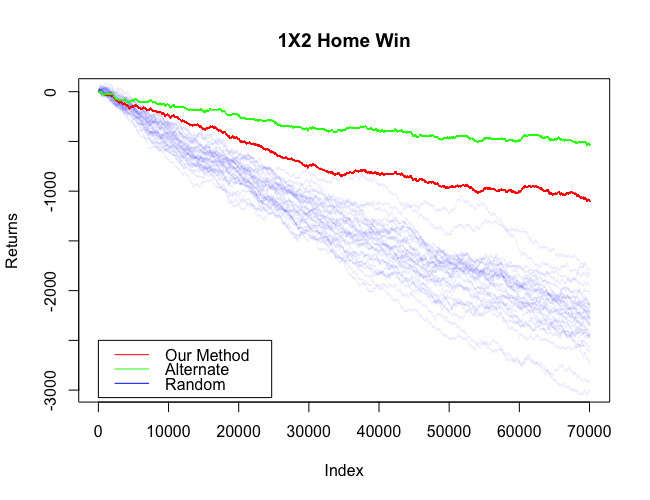
\includegraphics[width=.65\textwidth]{model_05_1x2H.png}  
	\caption{A line graph of the winnings of the random bet strategy in the 1X2 Home Win market, compared to the proposed algorithm and the \textit{alternate} method.}\label{FIG:03_03_randomstrat_1x2H}
\end{center}\end{figure}
\begin{figure}[h!]\begin{center}
	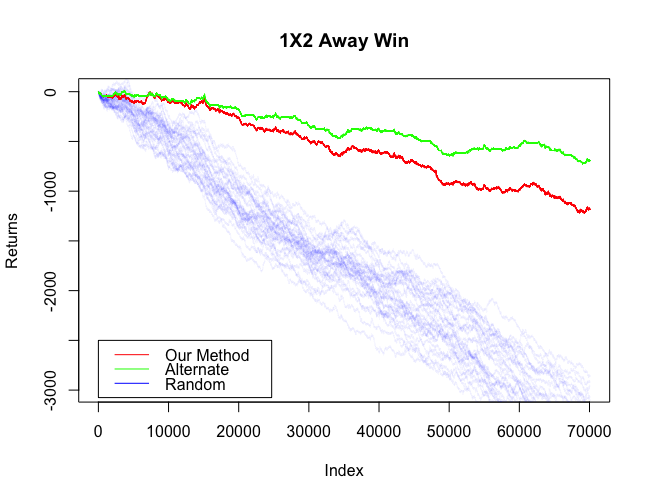
\includegraphics[width=.65\textwidth]{model_05_1x2A.png}  
	\caption{A line graph of the winnings of the random bet strategy in the 1X2 Away Win market, compared to the proposed algorithm and the \textit{alternate} method.}\label{FIG:03_03_randomstrat_1x2A}
\end{center}\end{figure}

\pagebreak

\begin{figure}[h!]\begin{center}
	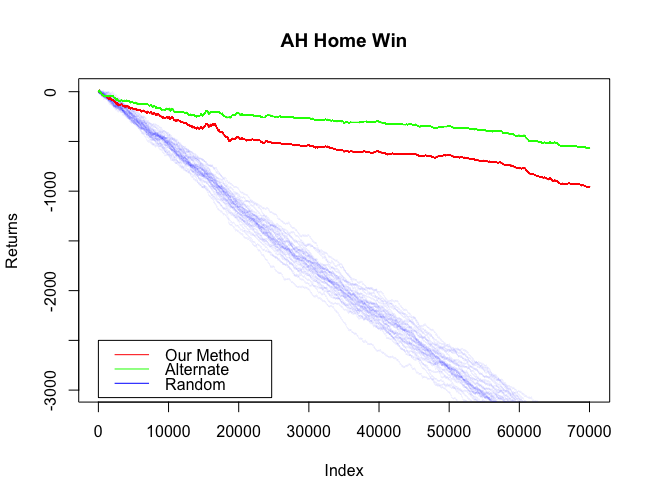
\includegraphics[width=.65\textwidth]{model_05_AHH.png}  
	\caption{A line graph of the winnings of the random bet strategy in the AH Home Win market, compared to the proposed algorithm and the \textit{alternate} method.}\label{FIG:03_03_randomstrat_AHH}
\end{center}\end{figure}
\begin{figure}[h!]\begin{center}
	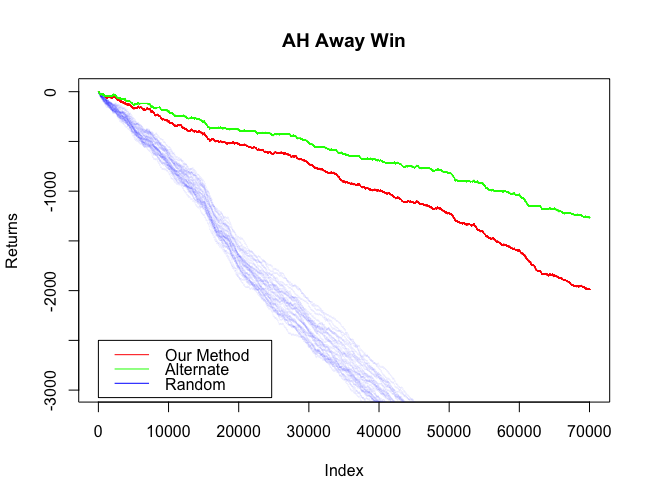
\includegraphics[width=.65\textwidth]{model_05_AHA.png}  
	\caption{A line graph of the winnings of the random bet strategy in the AH Away Win market, compared to the proposed algorithm and the \textit{alternate} method.}\label{FIG:03_03_randomstrat_AHA}
\end{center}\end{figure}

\pagebreak

The figures, and Table~\ref{tab:randombetstrategy}, show a clear trend. Whilst the proposed algorithm makes a loss, it is significantly better than the RBS, with the most significant improvements coming in the AH market. Figures~\ref{FIG:03_03_randomstrat_AHH} and \ref{FIG:03_03_randomstrat_AHA} display this, with a immediate and instant loss with the RBS. On average, the RBS lost 17.8\% and 17.7\% of the stake in the Asian Handicap markets, compared to 4.9\% and 7.5\% for the proposed algorithm in the corresponding markets: a difference of 12.9\% and 10.2\%. The accuracy, however, had less than 4\% difference in each market. 

Interestingly, the line for the RBS returns in the AH market had far less variation than the 1X2 market, which could suggest that, unless the bettor has a set strategy and/or insider knowledge, a loss of around 17.7\% is inevitable.

In the 1X2 market, despite vast decreases in accuracy (the RBS for the Home Win market was 19\% less accurate; the Away Win market was 17\% less accurate), the final winnings were not as poor as in the AH markets, with 2.8\% and 4.7\% larger losses. In addition, from the figures, the RBS has a larger distribution in the 1X2 markets, with some runs performing similarly to the proposed algorithm for a long time: in Figure~\ref{FIG:03_03_randomstrat_1x2H}, for example, two runs with similar results to the algorithm are observed until around Match Index 50000. The proposed algorithm always finishes more profitable than the RBS, however.

\section{Conclusion}\label{sec:modelconc}

The proposed algorithm outperforms the random bet strategy. In order to improve the results, with an aim to create a profit, however, more advanced methods, such as utilising maximum odds on offer for a match, vast amounts of data, or insider knowledge are required. It has been shown that a high level of accuracy doesn't equate to winnings, or that a vastly lower accuracy results in much lower profit. In addition, it was shown that the Asian Handicap market was harder to make winnings from than the 1X2 market, without either a being knowledgeable bettor, and/or utilising a more advanced model. 

It is, therefore, unsurprising that the bookmakers are so profitable: Entain---the owners of Coral and Ladbrokes---reported a £175 million profit in the year ending in 2020; Flutter---the owner of PaddyPower, Sportsbet, Betfair, and SkyBet---reported a profit of £136 million in 2019; and bet365 reported a profit of £560 million in 2019 \autocite{davies21, flutter, bet365revenue}. In addition, bookmakers are known to discriminate against successful bettors, often refusing bets to be placed, or even refusing to pay out large sums, thus making it even hard for bettors to make profits \autocite{symonds20, cave15, osborne15}.

\begin{center}\noindent\rule{0.5\textwidth}{0.6pt}\end{center}

In Chapter~\ref{ch:conc}, the findings made throughout the project are given together, as well as a personal reflection into what I have learnt throughout the course of the project.

\chapter{Conclusion}\label{ch:conc}
In this final chapter, the findings from this project will be discussed as well as areas for future research, and, from a self-reflecting view, challenges I have been faced with throughout the duration of the project, and how I overcame them.  

\section{Findings, Strengths, and Limitations}\label{sec:findings}
The aim of this project was to use a range of measures and methods to quantify bookmaker accuracy in football, across two different league groups (an \textit{elite} group of six top-tier European leagues and between different levels of the English \& Scottish pyramids), and across three popular markets (the 1X2, Under/Over 2.5 Goals (UO), and Asian Handicap (AH)). This was paired with investigations into the effect of competitive balance on accuracy and into the overround---a measure of bookmaker commission---set by bookmakers.

\subsection*{The 1X2 Market}
It has been shown that the bookmaker accuracy is high in the 1X2 Home Win and Away Win markets, based on visual analyses, and five measures of statistical accuracy: $R^2$, RMSE, $P_1$, $P_2$, and the Slope of the linear model created to find $R^2$ and RMSE. Bookmakers, however, struggle with the prediction of Draws, and opt to use a ‘safe’ method of setting relatively constant odds (the consensus probabilities have a low standard deviation), set to reflect the actual probability of a Draw occurring (approximately between 0.25 and 0.27, changing over time and across leagues). These findings are as expected. What is, perhaps, more unexpected is in the English \& Scottish pyramid analysis, bookmaker accuracy in all four measures was worse in the Level 2 group of leagues (English Leagues One and Two; Scottish Championship) than in the Level 3 group (English National League; Scottish Leagues One and Two). 

\subsection*{The Under/Over 2.5 Goals Market}
The UO market was shown to exhibit poor levels of accuracy from bookmakers, with an $R^2$ of 38.7\% and RMSE of 0.1478. It was shown to be improving over time, with four $R^2$ values greater than 75\% in the last five seasons considered. $P_1$ and $P_2$ steadily improved too, with the former rising from 0.5020 to 0.5039, and the latter decreasing from 0.4960 to 0.4923. Between levels, in the $R^2$ and RMSE variables, Level 1 and 2 appear to have similar performance: $R^2_{L1}=64\%$, $R^2_{L2}=53\%$ and RMSE$_{L1} = 0.1047$, RMSE$_{L2} = 0.1241$. Level 3 had much worse performance by these two measures, but appeared to perform better than Level 2 based on the $P$-values. 

\subsection*{The Asian Handicap Market}
It was shown via visual analysis (Figure~\ref{FIG:02_04b_count2}) that the handicap is well placed and is improving over time (the variance in odds offered is reducing, and approaching 0.5, ideal AH odds; Figure~\ref{FIG:02_7b_overroundah_season}). However, the market performance appears to be decreasing over time, with $R^2$ decreasing (in 2005/06, $R^2=81\%$ to, in 2019/20, $R^2=53\%$), RMSE increasing (0.1568 to 0.1605). The $P$-values appear to be worsening over time, too, with $P_1$ dropping from 0.5026 to 0.5006, and $P_2$ rising from 0.4948 to 0.4988. These values, however, still indicate slightly better performance in this market than in the UO market: the $R^2$ and RMSE values may be unreliable due to the lower variation in consensus probabilities making a linear model unsuitable. Between levels, bookmakers performed best in Level 1, across all four variables, followed by Levels 2 and 3, with a decrease in $R^2$ and $P_1$, and an increase in RMSE and $P_2$.

\subsection*{The Effect of Competitive Balance}
Competitive balance affects bookmaker accuracy. Three measures were used to quantify competitive balance; it was shown in leagues where balance is high (such as the French Ligue Une and German Bundesliga), bookmakers, whilst performing highly, performed relatively worse than in leagues where balance is low (Portuguese Primiera Liga).

\subsection*{Bookmaker Overround}
Bookmakers set a higher overround at lower levels; this is more evident in the 1X2 and UO markets. Over time, the overround is reducing in these two markets, whilst remaining stable in the AH market. It was found the AH handicap choice is improving, as the variation of consensus probabilities (and hence, odds offered) is reducing, and concentrating around 0.5.

\subsection*{Findings from the Proposed Betting Algorithm}
Whilst it did not perform as well as hoped, and ultimately made a loss in all four markets, a connection was made between the percentage of bets won, and the actual winnings of the bets. The algorithm won more bets than the successful method proposed by \citeauthor{kaunitz17} (\citeyear{kaunitz17}) yet lost a much greater percentage. To win money whilst betting, bettors without `insider’ knowledge therefore likely require large amounts of data \autocite{godin14} or advanced mathematical tools \autocite{dixon97, Owen09, karlis09, constantinou20}.

\subsection*{Strengths and Limitations of this Study}
This project established a possible link between competitive balance and accuracy, and reviewed a wide range of leagues, across multiple markets, using various measures.

Naturally, there are limitations to this piece of work. Firstly, the AH and UO markets could be assessed for the \textit{elite} group.\footnote{This was not done to create a `blind' environment for the algorithm in Chapter~\ref{ch:model}.} In addition, the data was from a limited range of seasons, 2005/06 to 2019/20, and with only a select group of leagues; for the investigation into bookmaker accuracy across levels, perhaps finding more data would have assisted the results. The $R^2$ and RMSE values used throughout are based on the creation of linear models: this may not have been the most appropriate choice of model, or the most appropriate choice of statistics. RMSE, for instance, computes the distance of a datapoint to the linear model, rather than the `perfect accuracy' $x=y$ line. The slope of the linear model is considered instead, though if a linear model is inappropriate, the slope is also inapplicable.

For the investigation into competitive balance, \citeauthor{Goossens05} (\citeyear{Goossens05}) uses data from the 1963/64 season until the 2004/05 season: the findings would be improved if the data coincided with the same seasons. In addition, the Top $k$ Teams statistic (named the kappa $\kappa$ value) uses an arbitrary choice of $k=3$ which may not accurately reflect balance over time: the English Premier League, for example, had a period of having a `big four' teams in the 2000s (Arsenal, Chelsea, Liverpool, Manchester United), before an ongoing period of a `top six' (with the additions of Manchester City and Tottenham Hotspur) \autocite{kelly21}.

Of course, this project has also left stones unturned and more questions to be asked, such as:
\begin{itemize}
	\item Does there exist a relationship between the style of play of a football league (whether the league is generally more offensive or defensive, or individual teams) and bookmaker accuracy?
	\item Has the COVID-19 pandemic affected bookmaker accuracy, or football itself (with changes to home advantage, for example)?
	\item Could it be possible for bookmakers to accuracy predict Draws?
	\item Is the competitive balance of the English \& Scottish lower professional leagues higher than that of the top-tiers, and semi-professional football? (This could explain why bookmaker accuracy is lower in the Level 2 leagues in Chapter~\ref{ch:ensco}.)
\end{itemize}

\pagebreak
\section{Challenges} \label{sec:challenges}

This project has tested my understanding of probabilities, odds, and various statistical techniques and tools. I used R to conduct my analysis, and my knowledge of which---despite having used it in several modules throughout my degree---has grown enormously over the course of the project, for example, dealing with programming problems and learning how to solve the plethora of issues that can occur, from simple syntax errors to issues with data types. At the start of the project, I was downloading every \lstinline|.csv| file from \url{football-data.co.uk} to use within my coding, which was very time consuming. Efficient methods, such as using \lstinline|for| loops regularly within the code helped massively. In addition, the use of the \lstinline|ggplot2| package has allowed me to create both a wider range of, and more aesthetically pleasing, plots: prior to the project, I had never used it before. Perhaps the most challenging code I used is the code to run the random bet strategy (Section~\ref{sec:modelcomp}), where I defined a new distribution (using the \lstinline|discrete| tool from the \lstinline|e1071| package) and ran the code numerous times: first to create the tables in Appendix~\ref{app:rbsruns}, second to create the plots in Figures~\ref{FIG:03_03_randomstrat_1x2H} to \ref{FIG:03_03_randomstrat_AHA}.

Formal critical analysis of literature has been something I have never done prior to the project, and something I initially struggled with. I found, after several constructive meetings, good techniques both for creating the Literature Review (Section~\ref{sec:litrev}) and for using findings within the project.

Project management has been crucial, too. Whilst the overall time frame is long, I found setting myself small goals and targets weekly or biweekly a great way of keeping on track, and continually making progress. Unlike other courseworks throughout university, there has been no set mark scheme/list of questions to follow, rather I have had to set the questions and aims myself.

Finally, this dissertation has tested both my \LaTeX\ skills, and communication, trying to ensure I present my findings clearly, concisely, and without unnecessary repetition. I hope I have managed to do this!



\pagebreak
\printbibliography
\appendix
\appendixpage

\chapter{Definitions}\label{app:definitions} 
\section{Mathematical and Statistical}\label{app:definitionsmaths}
\emph{Unless stated, these definitions have been taken from the Fifth Edition of the Oxford Concise Dictionary of Mathematics} \autocite{OxfordMathsDict}.
\renewcommand{\labelenumi}{(\roman{enumi})}
\begin{enumerate}
	\item \label{def:algorithm} \textsc{Algorithm} --- `A precisely described routine procedure that can be applied and systematically followed through to a conclusion.'
	
	\item \label{def:centrallimittheorem} \textsc{Central Limit Theorem} --- `[T]he distribution of the mean of a sequence of random variables tends to a normal distribution as the number in the sequence increases.'
	
	\item \label{def:cleaning} \textsc{Cleaning} (Data) --- Modification, removal, or replacement of `coarse' (`heaped, censored and missing') data \autocite{wu12}.
	
	\item \label{def:coeffofdet} \textsc{Coefficient of Determination}, $R^2$ --- For a linear model, with data points $x$ associated with a fitted value $f$ and residuals $e_i = y_i - f_i$. Then, $R^2$ is computed by finding the following:
	$$ \begin{array}{rcl}
	\textrm{The mean of the observed data, }\bar{x} &=& \frac{1}{n} \sum^{n}_{-1} x_i \\
	\textrm{Total sum of squares, }SS_{tot} &=& \sum_i (x_i - \bar{x})^2 \\
	\textrm{Sum of squares of residuals, }SS_{res} &=& \sum_i e_i^2
	\end{array}
	$$ 
	Then,
	$$R^2 = 1 - \frac{SS_{res}}{SS_{tot}} $$
	
	\item \label{def:confidenceinterval} \textsc{Confidence Interval} --- `An interval, calculated from a sample, which contains the value of a certain population parameter with a specified probability.'
	
	\item \label{def:discrete} \textsc{Discrete} --- `[I]t only takes values from a set of distinct values' (\textsc{i.e.}, not continuous).
	
	\item \label{def:distributions} \textsc{Distributions} --- `[This is] concerned with the way in which the probability of its taking a certain value, or a value within a certain interval, varies. It may be given by the cumulative distribution function[,] its probability mass function [or] its probability density function.'
	
	\item \label{def:fit} \textsc{Fit} --- `[T]he degree of of correspondence between the observations and the model's predictions.'
	
	\item \label{def:kerneldensityestimate} \textsc{Kernel Density Estimation} --- The `process of finding an estimate probability density function of a random variable. The estimation attempts to infer characteristics of a population, based on a finite data set. The data smoothing problem often is used in signal processing and data science, as it is a powerful way to estimate probability density. In short, the technique allows one to create a smooth curve given a set of random data' \autocite{kerneldensity}.
	
	\item \label{def:leverage} \textsc{Leverage} --- The amount of influence each data point $y_i$ can have on each fitted $y$-value, $\hat{y}_j$ \autocite{HoaglinWelsch78}.
	
	\item \label{def:lineofbestfit} \textsc{Line of Best Fit} --- ` A line through a scatter plot of data points that best expresses the relationship between those points' \autocite{lineofbestfit}.
	
	\item \label{def:mode} \textsc{Mode} --- `For a continuous random variable, [a mode is] a value at which the probability density function has a local maximum.'
	
	\item \label{def:normaldist} \textsc{Normal Distribution} --- `The continuous probability distribution wth a probability density function $f$ given by 
	$$f(x) = \frac{1}{\sqrt{2\pi\sigma^2}}\exp\bigg(-\frac{(x-\mu)^2}{2\sigma^2} \bigg) $$
	denoted by $\mathcal{N}o(\mu,\ \sigma^2)$' where $\mu$ is the mean and $\sigma^2$ the variance.
	
	\item\label{def:skewness}\textsc{Skewness} --- `The amount of asymmetry of a distribution... If the distribution has a long tail to the left[...] it is said to be skewed to the left and to have negative skewness.'
	
	\item \label{def:stddev} \textsc{Standard Deviation}, $\sigma$ --- `The positive square root of the variance, a commonly used measure of the dispersion of observations in a sample.'
	
	\item\label{def:standarderror}\textsc{Standard Error} SE --- `The standard deviation of an estimator of a population parameter.'
	
	\item \label{def:variance} \textsc{Variance} $\sigma^2$ --- `[...] equal to $E[(X-\mu)^2]$,' the expected value of the squared difference between an observation and the mean.
	
\end{enumerate}
\section{Gambling Terms}\label{app:definitionsgambling}
\begin{enumerate}
	\item\label{def:bettor} \textsc{Bettor} --- Someone who places a bet. Also \textit{punter}, \textit{gambler}.
	\item\label{def:bookmaker}\textsc{Bookmaker} --- Organisation that accepts and pays off bets. Also \textit{house}, \textit{bookie}.
	\item \label{def:calciopoli} \textsc{Calciopoli} --- A match fixing scandal which occurred in the 2004/05 and 2005/06 seasons, where Italian Serie A teams (AC Milan, Fiorentina, Juventus, Lazio and Reggina) `systematically influenced referees.' \autocite{Calciopoli}.
	\item\label{def:compbal} \textsc{Competitive Balance} --- `The situation in which no one business of a group of competing businesses has an unfair advantage over the others.' \autocite{CompetitiveBalance}.
	\item \label{def:disgraceofgijon} \textsc{Disgrace of Gijón} --- A football match between West Germany and Austria at the 1982 FIFA World Cup where a `mutually suitable scoreline' was played out, ensuring both sides progressed to the knockout rounds, leading to the final pair of subsequent World Cup group stage matches being played simultaneously \autocite{DisgraceofGijon}.
	\item\label{def:favelongshot} \textsc{Favourite-Longshot Bias} --- An anomaly in betting markets where the favourites win more often then the market probabilities imply; longshots less often \autocite{cain00}. 
	\item \label{def:overround} \textsc{Overround} --- `Bookmakers are business people and the prices they offer include a profit margin, which is sometimes referred to as the `vig' or `vigorish' in the prices they offer[...]. Overround is [...] defined as the sum of the reciprocals of all prices in a given market. Some definitions of overround subtract 1 from this sum' \autocite{overround}. \textsc{n.b.}, in this project, overround is defined without this subtraction.
	\item \label{def:stake} \textsc{Stake} --- The amount of money placed onto a bet by the bettor (the amount of money \textit{at stake}); \textit{the ante}.
\end{enumerate}

\chapter{Chapter 2 Code}\label{app:chap2code} 	\lstinputlisting{eliteleagues.R}
\chapter{Chapter 3 Code}\label{app:chap3code}	\lstinputlisting{ensco.R}
\chapter{Chapter 4 Code}\label{app:chap4code}	\lstinputlisting{model.R}

\chapter{Random Bet Strategy Runs}\label{app:rbsruns}
Tables for the \textit{random bet strategy} in Section~\ref{sec:modelcomp}, ran ten times, with an average taken found.\vspace{3mm}

\noindent For each run, the following variables are used as the column headings, in order:

\begin{tabular}{ll}
rand\textbf{xx} & the \textbf{xx}$^{\textrm{th}}$ run of the RBS.\\
bets & The number of bets placed.\\
stake & The number of units staked.\\
wins & The total winnings. \\
prop & The proportion return: defined as the winnings divided by the stake.\\
diff & The difference in the proportion return, between the RBS and Table~\ref{tab:betaccuracy}.\\
acc (pc) & The accuracy (\% of bets won), displayed as a percentage.\\
diff & The difference in the accuracy, between the RBS and Table~\ref{tab:betaccuracy}.
\end{tabular}

\small
\begin{center}
\noindent\csvautotabular{randombetstrategy/01.csv}\\
\csvautotabular{randombetstrategy/02.csv}\\
\csvautotabular{randombetstrategy/03.csv}\\
\csvautotabular{randombetstrategy/04.csv}\\
\csvautotabular{randombetstrategy/05.csv}\\
\csvautotabular{randombetstrategy/06.csv}\\
\csvautotabular{randombetstrategy/07.csv}\\
\csvautotabular{randombetstrategy/08.csv}\\
\csvautotabular{randombetstrategy/09.csv}\\
\csvautotabular{randombetstrategy/10.csv}\vspace{3mm}

\noindent Taking the average of each cell:\\
\csvautotabular{randombetstrategy/averages.csv}
\end{center}
\normalsize

\chapter{Project Diary} \label{app:diary} % Update whenever we have a meeting!
\section*{Meeting One --- 25/09/20}
Maha, Alun and I discussed the start of my project: how it will be assessed, what I need to do each week, \textsc{etc.} We spoke about where the data can be found (\url{football-data.co.uk}), how to import it, how to use it, and how it is formatted. We went over the basics of probabilities and their relationships with odds and the bookmaker's commissions (typically 5\%). Before next week, I will read the \citeauthor{kaunitz17} (\citeyear{kaunitz17}) and look at replicating the simple steps (means, standard deviations) with my data.

\section*{Meeting Two --- 02/10/20}
We reviewed the \citeauthor{kaunitz17} (\citeyear{kaunitz17}) paper, and looked at my R code used to complete the first steps. Before next week, I need to find out how \url{football-data.co.uk} source their data; do exploratory work on R (such as histograms and other basic plots) for either the 1X2 market across multiple seasons and leagues, or look at goals data for one league.

\section*{Meeting Three --- 09/10/20}
After Meeting Two, I made plots of observed vs. bookmaker probabilities using fixed points (this ended up with some very small bins): we discussed how it would be better to make sure the bin sizes are equal, instead. Maha spoke about the need for ensuring my code is well-commented, and to start properly writing up what graphs show (it will make my final write up easier). Finally, we realised \url{football-data.co.uk} renamed their \lstinline|BbAvH| column to \lstinline|AvgH|: I had come across problems with using data from multiple seasons.

\section*{Meeting Four --- 16/10/20}
We looked into problems I faced with previous code, caused by small sample sizes. The point was made that \lstinline|tapply| can be used to find the mean of a bin, rather than taking the midpoint, creating far more accurate plots and linear models. We discussed methods for comparing accuracy over time (statistics such as $R^2$, mean squared error, \textsc{etc}. or tests such as Kendall's Tau or Pearson's Rank), and spoke about the affect of \textit{competitive balance}, and how we can quantify it to use in part of our analysis.

\section*{Meeting Five --- 23/10/20}
With Alun, we spoke about what plots I have created showed, and how I can use them in my project as a point for discussion. We discussed why RMSE is a better measure of accuracy than mean square error, median square error or absolute square error. Alun also showed me some extra papers, such as \citeauthor{Owen09} (\citeyear{Owen09}), with methods and statistics ($P_1$ and $P_2$) that can be applied to the project. We discussed the future of the project, and how I will continue to progress. Finally, we spoke about the need to record everything I do, and to include more significant figures in my values for $R^2$.

\section*{Meeting Six --- 06/11/20}
Up until now, I had imported the \url{football-data.co.uk} datasets individually: Maha showed me a much better method using \lstinline|for| loops and the \lstinline|paste0| R command, which cut down a 1,000+ line document to around 100. We spoke about a number of papers I found about competitive balance, and the coefficients they used to quantify it. We spoke about using a binomial regression model, using $1/{O_i}$ (inverse of odds) as a predictor, and adding the season and leagues as additional ones, to see what affect they have. Finally, we spoke about what information would be included in my exploratory data analysis section.

\section*{Meeting Seven --- 13/11/20}
We spoke about using an ordinal logistic model, rather than binomial, and the pros and cons of each (OLM is simpler to code and run, but we may have multicollinearity between Home Win and Away Win probabilities). Alun demonstrated how the \texttt{ordinal} package worked, with the \lstinline|clm| and \lstinline|clmm| commands. We discussed whether or not the country would be treated as a fixed factor, and finally, we spoke about looking into how often the bookmakers `favourite' won, and different ways we could define this.

\section*{Meeting Eight --- 20/11/20}
Maha gave me information about the literature review, and how I could prepare for this: for each paper I use, write down a summary of the paper, including:
\begin{itemize}
	\item what the paper is about,
	\item how the researchers found the results (their method),
	\item the results they showed,
	\item and similarities and differences with my paper.
\end{itemize}
Maha recommended I create a table with these headings to fill in each time I use a new paper. We also discussed my ethical approval (the first check is on December 7$^{\textrm{th}}$ 2020). 

\section*{Meeting Nine --- 27/11/20}
Due to coursework deadlines, I hadn't done much new work on my project, so we went over my progress so far, and had a discussion about what I've shown so far. We concluded I'm making good headway into the project, and how I can improve my results. We discussed other packages and techniques I can use, such as the \lstinline|erer|, \lstinline|marginal| and \lstinline|mass| packages.

\section*{Meeting Ten --- 16/12/20}
Throughout the last week, I'd been working through a number of papers and summarising them (as per Maha's suggestion, Meeting Eight). We discussed what I need to show by the January check. I'd also made a number of plots using the \lstinline|ggplot2| package, which Alun and I went over, making a number of comments about them. We looked at changing the parameters for the density plot (default is Gaussian kernel estimate, and $n=512$). We discussed these plots at length and how the matches with a high probability of a Draw are likely due to match fixing or when a Draw suits both teams. At length, we discussed the difference in density plots for each league, and why some leagues appeared to have a unimodal distribution, and others having a trimodal distribution. Alun suggested using Odds Portal to check any unusual odds. We also discussed a tile plot I created, and discussed that grouping 5+ goals was key: small bin sizes are not helpful. I also gave a brief outline of possible sections for my first section, which we modified, and what progress I'm expected to make over Christmas. Finally, we discussed the Under/Over 2.5 Goals market, and the Asian Handicap market, and how I could look into the accuracy of these over the Christmas break, and throughout Semester Two. 

\section*{Meeting Eleven --- 18/01/21}
\subsection*{Code and Content}
Over the Christmas break, I'd made a section of code to find $R^2$, RMSE, $P_1$, and $P_2$ for each league that was 205 lines long: we discussed how a \lstinline|for| loop would be much better, like how we did to read in the data. For the tile plot, we discussed possible ways of including bin size: we both agreed inserting a table below would be clearest. Maha confirmed a question I had about including code in-text, rather than referring to it in the appendices. 

\subsection*{Write-Up}
In my submitted document, I couldn't get references to work: Maha recommended the \lstinline|natbib| \LaTeX\ package, and we spoke about how APA and Harvard are the best referencing systems. Maha also made it clear figures should be in the middle of the text, where they are needed in context, so the reader doesn't have to continually refer back and forth. A small conclusion at the end of each chapter is required, as well as a final concluding chapter with our findings and discussion. Figure labels need to be below the figure; table labels above. Maha also sent an annotated copy of my write-up.

\section*{Meeting Twelve --- 28/01/21} %Reference Shins? 
As well as making changes based on our previous meeting, I'd found a good paper discussing different leagues styles of play: as a result, I conducted principal components analysis with three new variables: \lstinline|predAcc| (predictive accuracy), \lstinline|imbalance| (a measure of the competitive imbalance in a league), and \lstinline|attack| (a measure based on the shots per goal: more shots implies a more attacking league). The Kruskal test is a good addition, as well as potentially running PCA on the seasons, rather than leagues. Finally, after Maha's comments on my draft about normalising the probabilities, I found Shin's Method of Normalisation \autocite{Strumbelj14}, which I will apply and compare over the next week.

\section*{Meeting Thirteen --- 16/02/21} %Maha off ill from here onwards
In the two weeks, I finalised my \textit{elite} data analysis, and moved onto the English \& Scottish leagues, including the Under/Over 2.5 Goals and Asian Handicap markets. The aforementioned Shin's Method was excluded, due to incorrect findings of consensus probabilities. Due to Maha being off ill, I caught Alun up with my progress, to which he made a few comments: I should look into the leverage of my models, especially with the Under/Over 2.5 Goals market; the $\chi^2$ test for independence between goals is good, but due to some expected values being low, I would need to group goals together: it also doesn't take into account the order of goals, so perhaps a different test (Spearman or Pearson) is better. Alun also introduced me to the Skellam distribution, based on the Poisson distribution, as a way to model goals, and recommended I read about bivariate Poisson distributions.

\section*{Meeting Fourteen --- 02/03/21} 
I made large amounts of progress in the two weeks, and started a new section, creating a betting model based on bookmaker's odds. Alun suggested making a few changes, such as changing the range of my bets for different markets and changing the units I bet on. We discussed ignoring the lower performing leagues and markets (such as German Bundesliga and Level 2 in the English \& Scottish leagues, and the U/O market). 

\section*{Meeting Fifteen --- 16/03/21}
Alun and I went through all of my outputs (figures, tables, \textsc{etc}.), and discussed what each one showed. He recommended I talk about the amount of coding knowledge I have acquired throughout the dissertation, and challenges I have faced throughout the course of the project, and how I have overcame them. We also discussed the presentation, and how I can both prepare for it, and what to include in it. 

\section*{Meeting Sixteen --- 30/03/21}
Alun and I discussed the final stages of the project. We went through my presentation slides, suggesting possible areas of improvement, and what needs to be included in my script. We went through what will be completed by the second check deadline, and what I will submit then, as well as a discussion into whether or not it is necessary to include the correlation tests in the dissertation (Kendall's Tau, Spearman Rank, and Goodman-Kruskal-Gamma tests): adding something with no value can make the dissertation harder to read. Finally, we spoke about the conclusion chapter, namely the inclusion of common themes and contradictory findings in it. 

\section*{Meeting Seventeen --- 13/04/21}
After a discussion about the presentation (when it would happen, what to include, \textsc{etc}.), Alun and I went through my April draft, looking at mistakes and things to chance, such as going into more depth at points, altering the Structure paragraph and discussing why I included certain steps. Finally, we concluded with a brief look at the progress I have made in the Model chapter, and what progress I need to make before submission. 

\section*{Meeting Eighteen --- 20/04/21}
Alun reviewed my draft of the Literature Review and Abstract, and going over my mistakes, such as discussing the importance of not referring to `we' in the Abstract. We then spoke about the presentation for a final time, ensuring the technology works and what to expect from the two markers. 


\chapter{Word Count} \label{app:wordcount}
Full word count: \textbf{20,307 words}\vspace{3mm}

\noindent\textbf{Breakdown:}\vspace{1mm}

\noindent\begin{tabular}{l|rrrr|r}
\textit{Chapter}	&\textit{Prose}	&\textit{Figures}&\textit{Tables}& \textit{Algorithms}	&\textbf{Total} \\
\hline
Abstract					& 270	& 		& 		&		& 270 \\
1: Introduction				& 3377	& 		& 246	&		& 3623 \\
2: \textit{Elite} Leagues	& 6095	& 110	& 679	&		& 6884 \\
3: English \& Scottish Pyramids& 4113	& 301	& 887	&		& 5301 \\
4: Proposed Method			& 1882	& 142	& 258	& 462	& 2744 \\
5: Conclusion				& 1485	& 		& 		&		& 1485 \\ \hline
\textbf{Total}				& 17222	& 553	& 2070	& 462	& \textbf{20307} 
\end{tabular}


\chapter{Ethical Approval Certificate} \label{app:ethics}

\noindent\begin{center}
\includegraphics[width=0.8\textwidth, trim={0 7cm 0 0},clip]{Certificate-114620.pdf}\end{center}
\end{document}
